\documentclass[a4paper]{report}
\usepackage{gillius}
\usepackage{helvet}
\usepackage{palatino}
\usepackage{newtxsf}
%\usepackage{fontspec}
%\renewcommand{\sfdefault}{Helvetica Neue} %doesnt work
\renewcommand{\familydefault}{ppl} %changes font, put in comments to go back to default font.

\setcounter{secnumdepth}{1} % only chapter and sections will be numbered
\setcounter{tocdepth}{1}    % entries down to \subsubsections in the TOC

\usepackage[titletoc]{appendix} %Adds word 'Appendix' to appendix titles in TOC
\usepackage{parskip} %Adds breaks between paragraphs
\usepackage[utf8x]{inputenc} %Encoding
\usepackage[T1]{fontenc} %Makes sure fonts and symbols
\usepackage{apacite} %Workaround to make nice citations work with natbib
\usepackage[longnamesfirst,sort]{natbib} %Adds citation style management
\usepackage[nottoc]{tocbibind} %Adds bibliography to the table of contents
\usepackage{color} %Adds the colour support, e.g. so I can add coloured comments 
\usepackage{framed} %Adds the frame support
\usepackage{setspace} %Adds line spacing control
\usepackage{a4wide} %Adds smaller margins
\usepackage{graphics,subcaption} %Pictures support; I CHANGED subfigure to subcaption for subfigures, check if everything still works.
\usepackage{sectsty} %Adds control over headings' fonts
\usepackage[framemethod=tikz]{mdframed} %Adds control over nice customisable text boxes
\usepackage{enumitem} %Adds customisation of item lists
\usepackage{pifont} %Adds access to special chars like the ones I use in the chapter summary boxes
\usepackage[font=small,labelfont=bf,font=sf]{caption} %Adds control over the captions
\usepackage{booktabs,array,ragged2e,multirow} %Adds more control over tables
\usepackage{float} %Adds more control over floats (figures and tables)
\usepackage{fancyhdr} %Adds control over the page headers
\usepackage{pgfkeys} %Allows to define own names
\usepackage{tikz} %Adds charts
\usepackage[bottom = 3cm]{geometry} %Helps with diagrams in general + set up margins
\usepackage{soul} %Adds strikethroughs
\usepackage{mathtools} %Adds math stuff - I use it to get the chi and eta symbols
\usepackage{lscape} %Adds vertical tables
\usepackage{moresize} %Adds HUGE fonts


\usepackage{pifont} %Adds checkmarks and crosses, which are defined in formatting.tex
\newcommand{\cmark}{\ding{51}}%defines the checkmark
\newcommand{\xmark}{\ding{55}}%defines the cross

\usepackage[hidelinks]{hyperref}
%\usepackage{hyperref} %This package should be added last apparently
%%\hypersetup{
%	pdftex,
%	colorlinks=false,
%	pdfpagemode=UseOutlines,
%	pdftitle={},
%	pdfauthor={ADD NAME}
%	}
\usepackage{hypcap}
 %document settings
%\includeonly{./settings/preamble, ./settings/title, ./settings/formatting, ./tex/ch34} %If I only want to compile certain chapters.

\begin{document}
%%%%%%%%%%%%%%%%%%%%%%%%%%%%%%%%%%%%%%%%%
% University Assignment Title Page 
% LaTeX Template
%
% This template is made and modified by Judith Borghouts based on a template downloaded from:
% http://www.latextemplates.com
%
% Original author:
% WikiBooks (http://en.wikibooks.org/wiki/LaTeX/Title_Creation)
% 
% Instructions for using this template:
% This title page is presently capable of being compiled as is. This is not 
% useful for including it in another document. To do this, you have two options: 
%
% 1) Copy/paste everything between \begin{document} and \end{document} 
% starting at \begin{titlepage} and paste this into another LaTeX file where you 
% want your title page.
% OR
% 2) Remove everything outside the \begin{titlepage} and \end{titlepage} and 
% move this file to the same directory as the LaTeX file you wish to add it to. 
% Then add \input{./title_page_1.tex} to your LaTeX file where you want your
% title page.
%
%%%%%%%%%%%%%%%%%%%%%%%%%%%%%%%%%%%%%%%%%

%----------------------------------------------------------------------------------------
%	PACKAGES AND OTHER DOCUMENT CONFIGURATIONS
%----------------------------------------------------------------------------------------


%\begin{document}

\begin{titlepage}

\newcommand{\HRule}{\rule{\linewidth}{0.5mm}} % Defines a new command for the horizontal lines, change thickness here

\center % Center everything on the page


%----------------------------------------------------------------------------------------
%	TITLE SECTION
%----------------------------------------------------------------------------------------

\HRule \\[0.4cm]
{\Large \bfseries Task, Interrupted: Understanding the Effect of Time Costs on Task Interruptions During Data Entry
}\\[0.4cm] % Title of your document
\HRule \\[1.5cm]
 
%----------------------------------------------------------------------------------------
%	AUTHOR SECTION
%----------------------------------------------------------------------------------------

\begin{minipage}{0.4\textwidth}
\begin{flushleft} \large
\emph{Candidate:}\\
Judith \textsc{Borghouts} % Your name
\end{flushleft}
\end{minipage}
~
\begin{minipage}{0.4\textwidth}
\begin{flushright} \large
\emph{Supervisors:} \\
Dr. Duncan \textsc{Brumby} \\% Supervisor's Name
Prof. Anna \textsc{Cox}
\end{flushright}
\end{minipage}\\[4cm]



% If you don't want a supervisor, uncomment the two lines below and remove the section above
%\Large \emph{Author:}\\
%John \textsc{Smith}\\[3cm] % Your name

%----------------------------------------------------------------------------------------
%	DATE SECTION
%----------------------------------------------------------------------------------------

{\large \today}\\[3cm] % Date, change the \today to a set date if you want to be precise

%----------------------------------------------------------------------------------------
%	WORD COUNT
%----------------------------------------------------------------------------------------

%Word count: 23081 as counted by detex dissertation.tex $ | $ wc -w

%This includes the report and appendices.

\begin{minipage}{\textwidth}
A dissertation submitted in partial fulfilment of the requirements for the degree of: \\

\textbf{Doctor of Philosophy of University College London} \\

UCL Interaction Centre,\\
Department of Psychology, \\
University College London
\end{minipage}
~

\vfill % Fill the rest of the page with whitespace

%----------------------------------------------------------------------------------------
%	HEADING SECTIONS
%----------------------------------------------------------------------------------------

%\textsc{\LARGE University of York}\\[1.5cm] % Name of your university/college
\begin{flushright} \large

\includegraphics[width=\textwidth]{images/logo.pdf}%\\[1cm]  % Include a department/university logo - this will require the graphicx package
\end{flushright}
%\textsc{\Large Department of Computer Science
%}\\[0.5cm] % Major heading such as course name

%\textsc{ Submitted in part fulfilment of the degree of the requirements for the degree of:}\\[0.5cm] % Minor heading such as course title

 
%----------------------------------------------------------------------------------------




\end{titlepage}
%\end{document} %title page

\setcounter{tocdepth}{2} %TOC depth

\setlength{\parindent}{0cm} %No indentation
%\doublespacing %Double spacing between lines
\setcounter{secnumdepth}{2} %Adds section numbering to subsub sections (default is 2)
\allsectionsfont{\sffamily} %Turns headers into sans-serif font
\interfootnotelinepenalty=10000 %Footers can't be split between pages

%Page headers with a chapter name and page numbers
\pagestyle{fancy} 
\fancyhf{}
\fancyhead[L]{\sffamily\nouppercase{\leftmark}}
\fancyhead[R]{\thepage}

\newlist{myitemlist}{itemize}{1} %Creates a new item list and defines the list styles for the chapter summary boxes
\setlist[myitemlist,1]{label=\ding{118},before=\raggedright}

\setitemize{partopsep=\topsep}
\setitemize{topsep=0pt}

%Defines borders for \fbox (which I sometimes use for figure borders)
\setlength\fboxsep{0pt}
\setlength\fboxrule{0.5pt}

\usetikzlibrary{shadows} %Adds shadows to the chapter summary box
\usetikzlibrary{arrows,decorations.pathmorphing,backgrounds,fit,positioning,shapes.symbols,chains, patterns} %Helps to draw diagrams

%Allows to use \& within symbolic coords
\let\OrgAmp\&
\protected\def\&{%
  \ifincsname
    \string\&%
  \else
    \OrgAmp
  \fi
}

%Create a new element - the chapter summary box
\newmdenv[
%shadow=true,
%leftline=false,
%rightline=false,
linewidth=1pt,
backgroundcolor=blue!10,
font={\fontfamily{cmss}\selectfont},
%\setmainfont{Gill Sans MT},
innertopmargin=10pt,
innerbottommargin=20pt,
innerrightmargin=20pt,
]{mynote}

%\newmdenv[
%shadow=true,
%font={\sffamily},
%innertopmargin=10pt,
%innerbottommargin=20pt,
%innerrightmargin=20pt,
%]{mynote} 

%Table styles
\renewcommand{\arraystretch}{1.5} %Adds spaces between rows to all tables
\newcolumntype{P}[1]{>{\RaggedRight\hspace{0pt}}p{#1}} %Makes sure that things like p{3cm} are left-aligned
\newcolumntype{C}[1]{>{\Centering\hspace{0pt}}p{#1}} %Makes sure that things like C{3cm} are centred


 %formatting settings

\section*{Abstract}
\addcontentsline{toc}{chapter}{Abstract}
Computer-based work often involves looking up information from different sources. Though these interruptions are required to progress with work, switching away from a task can be disruptive: it slows people down, increases errors and it is challenging to remain focused on work. This thesis investigates how interruption management tools can better support people in managing these types of work-required interruptions in the context of data entry work.

The first part of the thesis reports two qualitative studies looking at understanding data entry in an office setting. They demonstrate that physical interruptions are postponed until a convenient moment in the task if they are expected to take time, but digital interruptions are addressed immediately as these are presumed to be quick. The second part of the thesis reports three controlled experiments to test the hypothesis that people manage interruptions by avoiding time costs. They show that if people are able to learn the expected time costs of digital interruptions, they avoid interruptions with a high time cost by reducing the number of these interruptions and postponing them until later in the task, addressing interruptions with low time costs first. The third part of the thesis reports an online experiment and a field study that evaluate a design intervention showing people the duration of their interruptions. These studies show that showing people the time costs of digital interruptions makes people reflect on what they were doing during an interruption, reduces the duration of interruptions, and made people faster and more accurate in completing data entry tasks.

%The first part of the thesis describes two qualitative studies looking at the context in which office workers in finance offices perform data entry tasks. These studies reveal that participants often have to self-interrupt to collect information from both physical and digital sources. Whereas physical interruptions are postponed if these are expected to take time, digital interruptions were always addressed immediately as these were presumed to be quick. Observations however revealed that these could take much longer than expected, which suggests people are not aware of the time they spend on digital interruptions. 
%The second part of the thesis reports three controlled experiments to test the hypothesis that people prioritise collecting information according to expected time costs. These studies show that, in a controlled setting where participants can learn the time costs involved in accessing information, they first switch to information sources that are fast to access, and switch more frequently to these sources. On the other hand, people either prepare or postpone looking up information which takes time.
%The third part of the thesis evaluates whether giving people feedback on the duration of interruptions can influence people's switching strategies and data entry performance. An intervention was developed and evaluated with both an experimental data entry task and people's own data entry work. Together these studies show that feedback made people reflect on what they were doing during interruptions, it shortened the duration of interruptions and reduced errors and made people faster.

This thesis demonstrates that people manage interruptions based on expected time costs, and that giving people feedback on the time they spend on interruptions can help them manage their interruptions better. It makes a theoretical contribution by showing how people adapt to small changes in time costs by reducing the number and duration of interruptions, and postponing them until later in a task. It makes a practical contribution by showing how giving people feedback on time costs can help them in reducing the duration of interruptions, and improve people's focus. 
\section*{Impact statement}
\addcontentsline{toc}{chapter}{Impact statement}

The work presented in this thesis has impacts both inside and outside academia. 

Within academia, this thesis has increased our understanding of how time costs affect how people manage self-interruptions to look up information. These interruptions are addressed straight away if they are presumed to be quick and it is considered part of the activity, but it is hard for people to predict time costs outside of a controlled setting. Interruptions can take much longer than expected, which increases their disruptiveness to work. My thesis demonstrates that showing people how long they go away from a specific task helps people reduce the length of their interruptions, which can inform future work on understanding and controlling interruption behaviour. The findings have been published and presented at HCI conferences, universities and research labs. 

The findings also make an impact to the methodology of future data entry research, by demonstrating that for some types of data entry work, a major component is collecting data which impacts how data is entered. If data entry interfaces are to be used in situations where information is not readily available, they should be evaluated  by requiring participants to collect data from the environment. As part of this thesis I developed a new experimental task, which can be used in future data entry studies to investigate time costs of collecting data during a data entry task.

Outside academia, the findings of this thesis have a direct impact on developers of interruption management tools. This thesis contributes to our understanding of how awareness of time spent on technology can help people manage their use of time. Time management of technology use is a current issue: various technology companies have started to introduce features in 2018 to show how much time is spent in their applications, to encourage users to adopt healthier technology habits. My work contributes to addressing this issue by demonstrating how time awareness can not only help to regulate work-irrelevant technology use, but also to manage task-relevant interruptions during work. As part of my thesis, I have developed and evaluated a browser extension showing how much time the user spends away from a task: the extension is publicly available online to download and use. 
%\include{./tex/publications}
\section*{Acknowledgements}
\addcontentsline{toc}{chapter}{Acknowledgements}

First of all, many thanks go to my supervisors Duncan Brumby and Anna Cox for being such a great supervisory team. Duncan for challenging me on why I am doing things the way I do, and Anna for questioning how these things contribute to the big picture. Their guidance, feedback and support have helped me ensure my work was held to a high standard.

%But most of all, thanks for being accessible and available at all times. 

Thanks to Ann Blandford for examining my first-year and upgrade vivas. The feedback was critical in shaping this thesis.

%I also owe a big thank you to
I would also like to thank everyone at UCLIC - being surrounded by such an amazing group of people made the PhD a lot less lonely, and I will miss the daily lunches, chats, and laughs. Thanks to Sarah and Sandy for all their helpful advice when I got started, and for sharing my enthusiasm about data entry and interruptions - which admittedly is a niche thing to get excited about.
Thanks to Louise for always helping out with various things and making sure everything runs smoothly.
And thank you to all academics I had the opportunity to work with on the MSc course, for teaching me about teaching.

During the last part of my PhD, I was fortunate to work at Microsoft Research. Having breaks from my PhD, and being able to collaborate with various researchers approaching problems from different perspectives, helped me go back to my research with a fresh and refocused look. In particular thanks to my mentors Kenton O'Hara and Andy Gordon for always challenging and encouraging me to improve. 

I would also like to thank my MSc supervisor Paul Cairns: my master's project on number entry in 2013 was what inspired me to pursue a PhD in data entry at UCL. 

%Thanks also to David McKee, for proofreading parts of this thesis. 

The studies in this thesis depended on participants, and I am very grateful for their time and willingness to take part in the studies.

Thanks to my friends for their support, being a listening ear and being understanding regarding my erratic work schedule - I am sorry for all the events I have had to miss last-minute!

Throughout my life Taekwondo has been a fundamental part of my routine. These past years it has played an essential role in maintaining a healthy work-life balance, and in providing a much needed stress release. For this I owe thanks to everyone at my Taekwondo club, especially my coach Amar. Thank you all for the training sessions, competitions, for shouting at me, and for truly being one big family. 

Finally, I would like to thank my parents, my sister, and everyone else in my family for their unconditional love and support in all of my pursuits. Their trust and words of encouragement have helped me follow my instinct and pursue what I love to do, no matter where in the world it may take me.

\tableofcontents

\listoftables
\listoffigures

%\include{abbreviations}

\chapter{Introduction}

\begin{mynote}
\subsubsection{Chapter outline}
In this chapter, I introduce the problem which forms the motivation of this thesis. I outline the scope and the research questions it aims to answer, give an outline of the structure of the thesis, and present the proposed contribution.
\end{mynote}

\vspace{10pt}

\section{Motivation}

Imagine, you have just come back from a business trip and have to claim back your expenses. You collect your receipts from your wallet, open the expenses system, and start entering the items and prices into the system. The prices are in a foreign currency, so you leave the expenses system to go to a currency converter website and convert the prices. You then need to enter a budget code, which was sent via email a few months ago. Upon opening your email inbox, you see a new incoming email that captures your attention. How many times did you stop entering to go and look up certain information? And how long did this take you? You may have entered information that was easy to retrieve first, and left information that would take time to find until the end. And did you retrieve the budget code from your inbox and return to the expenses system straight away - or did you open that unread email instead? Whatever way you chose to complete the task, it involved making decisions on how to manage interruptions to look up required information for the entry task. 

Interruptions like these, called inquiries \citep{Jin2009}, happen when a person goes to look up information to aid the completion of a primary task. These interruptions are common, and many computer tasks require switching between  different information sources \citep{Cangiano2009}. The longer and more frequent these interruptions are, the more disruptive they can be: it takes time to resume the main task, it is challenging to remain focused, and it increases likelihood of errors. Furthermore, people can be triggered to further self-interrupt their work for other off-task activities \citep{Jin2009}. As a result, there now exists a large number of tools that aim to support people in avoiding digital distractions \citep{Lyngs2018}: for example, a common approach is to temporarily block interruptions \citep{Kim2017}. However, interruptions to look up information cannot be blocked, as these are needed to progress with the current task. Furthermore, interruptions can also be beneficial: they can boost mood and productivity \citep{Mark2014a}, and when information is found quickly, this can positively impact people’s work \citep{Jin2009}. In addition, a recent study showed that blocking distracting sources at the workplace caused office workers to work longer periods of time without any breaks, with higher stress \citep{Mark2018}.

In this thesis, I propose that for inquiry type interruptions, it is better to provide people with tools to self-regulate their behaviour, so they can learn how they can best allocate their time. To date, there have been insufficient tools available for this purpose. Commercial tools such as RescueTime and ManicTime track computer usage to allow users to view and reflect on their behaviour, but these tools give information about the user’s entire computer usage: interview studies revealed that users feel the data lacks context, and it is often not clear what to do with this data \citep{Collins2014}. A recent trend suggest that recent time spent on activities can be used to help regulate non-work activities: Whittaker et al \citep{Whittaker2016} showed that presenting the last 30 minutes of activity reduced time spent in emails and social media. More recently, social media have seemed to tap in on this trend by making features available showing how much time you spend in their app \citep{Instagram}. What is unknown is whether time affects work-relevant interruptions. Different inquiries take different time: information may be a few clicks away, or time has to be spent searching for this information. Are people aware of the time they spend on interruptions, and do they take this into account when managing interruptions? This thesis investigates how different time costs affect how people manage self-interruptions to look up information for a data entry task, with the aim to inform the design of interruption management tools.

%This thesis investigates how time costs influence people’s self-interruption behaviour. Prior work suggests that people try to minimise time when completing tasks: people make fewer interruptions to information if these interruptions take a long time \citep{Gray2006}. 

%In particular self-interruptions are difficult to regulate. Therefore, various interventions have been evaluated to decrease the disruptiveness of interruptions: interruptions are blocked, or people are given reflective information on what they are doing. However, it is unclear how people can manage interruptions that are needed for work, and people do not know what to do with reflective information. 

%Data entry
%Data entry is usually a straightforward task, but when information has to be retrieved from multiple sources, not all of which are as easy to access, this simple task can quickly become complex. Interrupting a data entry task to look up the required data can be disruptive, as you have to pay a time cost each time you resume your data entry task. You may have forgotten where you were, enter information in the wrong place, or misremember what you were supposed to enter and enter something incorrect. This disruption can introduce data entry errors, the outcomes of which can range from annoying to more serious consequences, such as transferring money to the wrong bank account, or transferring a wrong amount.  
%Because it is important data entry is done accurately, data entry research has looked at improving the input interfaces \citep[e.g.][]{Oladimeji2013, Vertanen2015, Wiseman2013a}, but it is not clear its design implications generalise to the type of situation as described above. In this situation, you do not enter all items from a source nearby, as in most data entry studies, but need to retrieve and enter different types of information (e.g. numbers, alphanumeric strings, words) from multiple sources (e.g. e-mails, paper receipts, different computer windows). The time cost to access these resources varies, and if information becomes harder to access, people increasingly rely on what they have memorised of the information rather than recheck the resource \citep{Gray2006}. It is however not known how people prioritise and manage their tasks when they have to retrieve the information from multiple resources, with varying access costs, or how a data entry interface should be designed to support people in these situations. 
%While it has been shown how changing the design of a data entry interface can affect and improve how we enter data, and that different information access costs affect how often people consult one source, it is not known how the interface can support situations when data has to be retrieved and entered from various sources with varying information access costs. In order to design interactive systems that truly support this type of data entry task, it is necessary to get a detailed understanding of how users manage this task and its subtasks, and to what extent the access to the required resources affect their strategies.

\section{Aim and scope}
The aim of this thesis is to understand how the disruptiveness of inquiries needed for a data entry task can be reduced. To achieve this aim, this thesis addresses the following research question:

\textbf{How can interruption management tools support people in managing inquiries for a routine data entry task, given variable time costs of required inquiries?}

To answer this question, a good understanding is needed of people's current interruption strategies, and to what extent these are influenced by different time costs. Therefore, the research question is addressed by answering the following subquestions across three chapters:

\begin{enumerate}
\item How do people manage inquiries for data entry in a finance office setting? (Chapter 3)
\item Do time costs affect the number, duration and timing of inquiries for data entry?  (Chapter 4)
\item Does time feedback affect the number and duration of, and awareness of time spent on, inquiries for data entry? (Chapter 6)
\end{enumerate}

These questions are best answered by using a mixed methods approach. To get a detailed understanding of how people currently manage inquiries, a qualitative approach can get an understanding of underlying reasons as well as how it is conducted in practice [source]. However, to be able to make claims about whether differences in behaviour is due to different time costs, a more quantitative approach is needed [source].  
Therefore, this thesis uses a combination of the following qualitative and quantitative methods:

\begin{itemize}
\item Interviews are used to get a first understanding of people's data entry work.
\item Observations and think-aloud protocols are used to get an understanding of how people currently manage inquiries for data entry work and why. 
\item Lab experiments are used to investigate to what extent interruption behaviour can be attributed to a difference in time costs of inquiries. 
\item An online experiment was used to investigate whether a design intervention that shows the duration of interruptions can affect people's self-interruption behaviour in an uncontrolled setting. 
\item A field study with semi-structured interviews was used to explore how applicable the design intervention would be for people's own data entry work. 
\end{itemize}

%\begin{enumerate}
%\item Does the IAC of information sources affect how people manage subtasks to look up information for an expenses task in a finance office setting?
%\begin{enumerate}
%\item	What (types of) information do people need for entering expenses?
%\item	Where do people need information from?
%\item	How do they address those needs?
%\item	Does the type of information, and where they need it from, affect how people address these needs?
%\end{enumerate}
%\item	How can the existing data entry system be redesigned to support or better support people managing subtasks of looking up information for entering expenses, given variable IACs for required information sources?
%\end{enumerate}

%Specific task and setting
For the scope of this thesis, I primarily focus on office workers in financial administration offices conducting data entry work. This task requires entering different types of information from a variety of sources, such as paper, spreadsheets, emails and databases. It is important the task is done accurately but within a reasonable amount of time as they are under time pressure to finish work on time. This task and setting is therefore considered to be an appropriate and interesting example to study further. The task serves as an example of a wider class of routine computer-based tasks, and it can be imagined findings of this thesis can be useful and generalise to other, similar, tasks that require frequently going and out of documents to collect information. For example, people who have to fill in their tax returns have to similarly enter a range of information into a computer system, and have to collect this information from multiple sources with varying time costs.

%Specific type of interruption
In this thesis, I am also primarily interested in inquiries, a particular type of self-interruption triggered by the need to look up task-related information. 
In the qualitative studies, I do consider how participants address interruptions overall, and the proposed design intervention may be used for all types of self-interruptions. However, the development of the design intervention was mainly based on the knowledge of how people address inquiries. Different types of interruptions have different triggers and impacts on task performance \citep{Jin2009}. It was therefore considered important to make a distinction between different self-interruptions, and pose restrictions on the scope of the thesis, to make a valuable contribution.

\section{Thesis outline}
Chapter 2 discusses related literature. It first discusses prior research on interruptions at the workplace, on information seeking and management, and technology interventions to address interruptions and information management. It also gives an overview of prior data entry research. This literature review highlights that it is important to get a detailed understanding of data entry work in its situated context, in order to support people in managing inquiries during data entry. 

Chapter 3-6 describe seven studies conducted to address the research question of this thesis. Chapter 3 describes two qualitative studies aimed to get a detailed understanding of data entry work in a finance office setting. These studies revealed that a major part of data entry is retrieving information from multiple sources with varying time costs. Chapter 4 reports three laboratory experiments to test the hypothesis that time costs influence the number, duration and timing of inquiries for a data entry task. These studies showed that people postpone interruptions with high time costs. Chapter 5 explores different design ideas, based on the research findings so far and prior literature. It describes the development and design of a browser notification which is based on the premise that showing time costs to users may help people manage interruptions outside a controlled setting. Chapter 6 describes an online experiment and a field study to evaluate the effectiveness of this browser notification showing the time costs of interruptions during data entry work. These studies showed that making people more aware of time costs can act as a trigger to reflect on what they were doing during prior interruptions, and encourages them to shorten their interruptions.

Chapter 7 summarises the key findings of the studies. It discusses the contribution that these findings make to knowledge and what the practical implications are. It also discusses opportunities for future work. 

The thesis structure is depicted as a diagram in Figure \ref{fig:ch1-thesisoverview}.

\begin{figure}
\centering
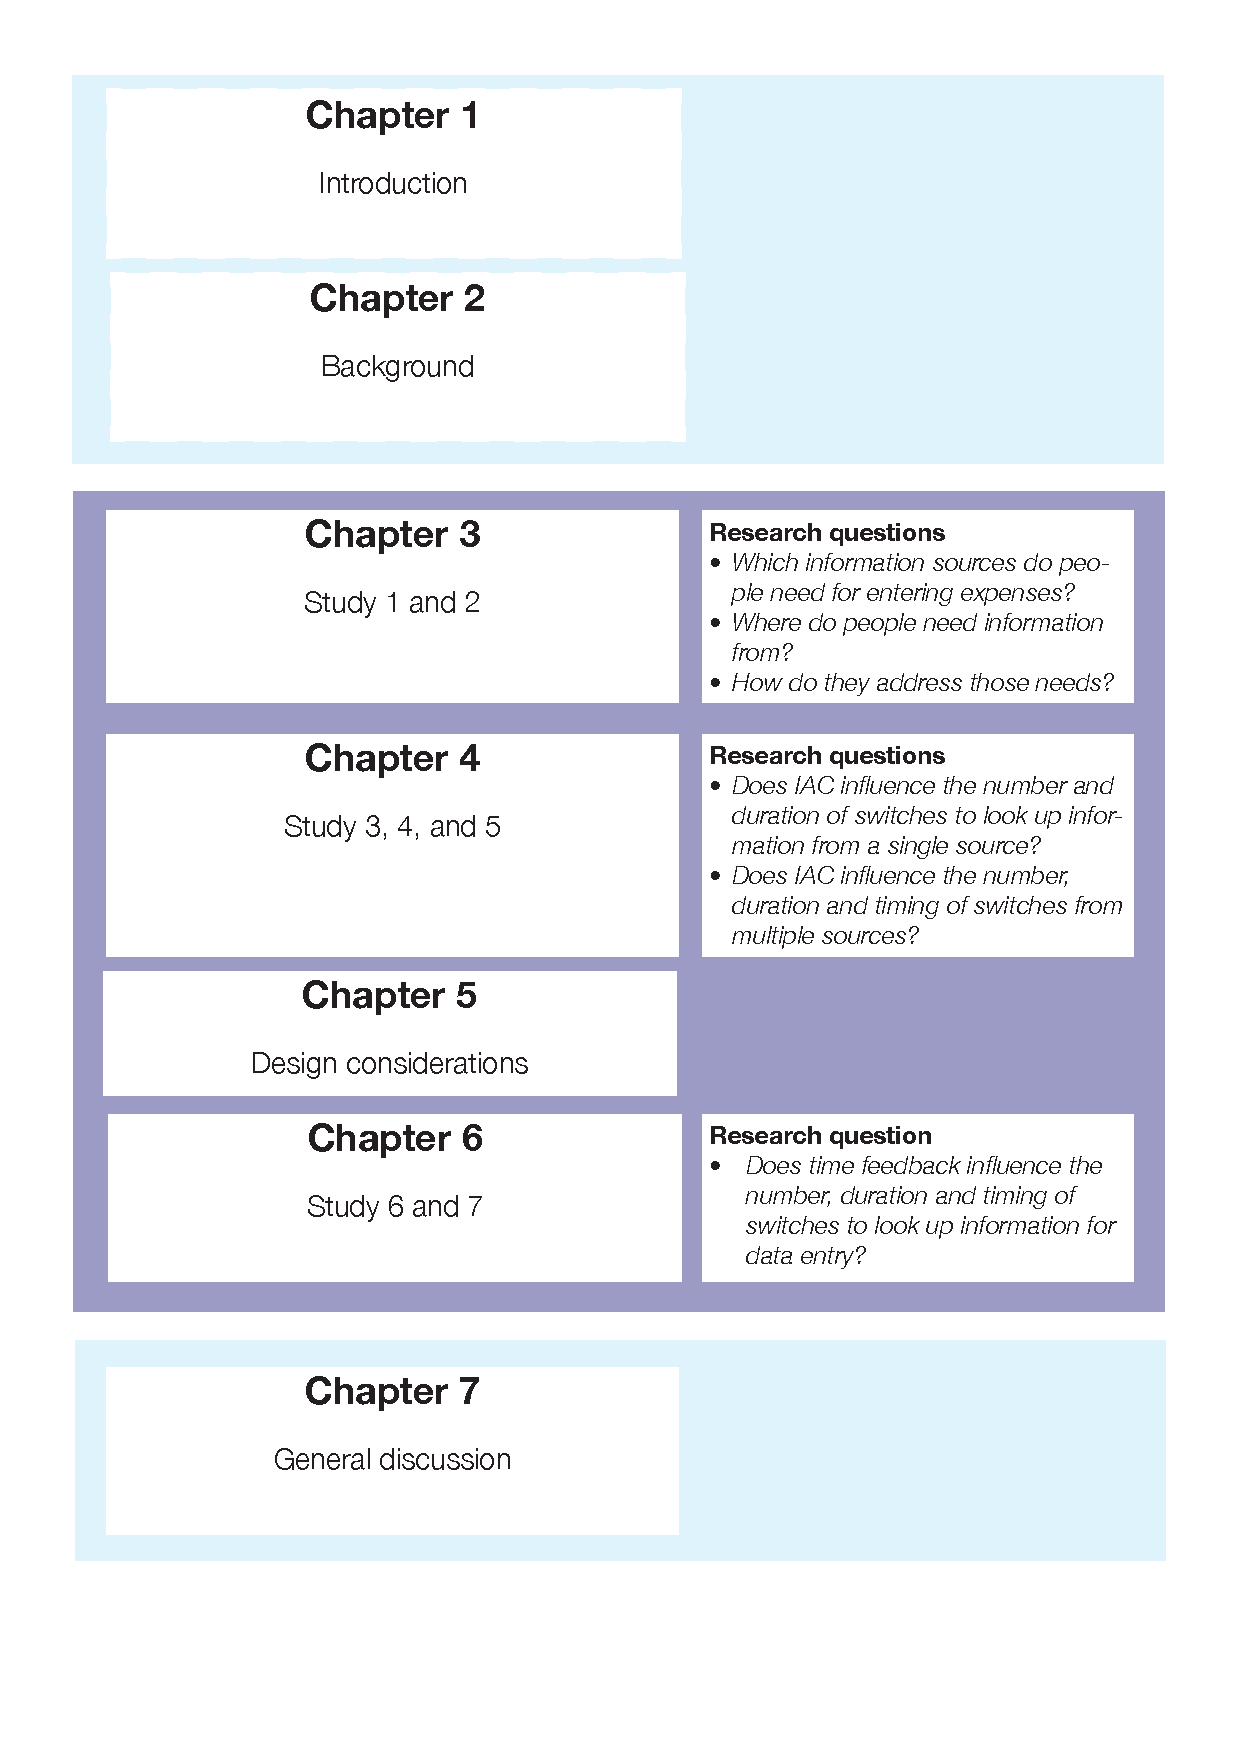
\includegraphics[width=0.7\textwidth]{images/ThesisOverview.pdf}
\caption{Visual overview of the thesis structure.}
%\vspace{-3pt}
\label{fig:ch1-thesisoverview}
\end{figure}

\section{Contribution}
%The thesis makes important contributions to knowledge as well as practical implications. 
%Knowledge
The first contribution of my thesis is an increased understanding of the effect of time costs on people's self-interruption behaviour to collect task-related information. Prior work has shown that longer interruptions are more disruptive than short ones, but to date it was unclear how time costs affect people's decisions when and whether to address self-interruptions. My thesis demonstrates that the presumed time cost of an interruption determines whether an interruption is addressed straight away (if it is presumed to be short), or if it is postponed until a more convenient moment in the task (if it is presumed to be long). I also show that in a controlled environment, people are able to learn the time costs of digital interruptions and adapt their strategies to first address interruption with a low time cost, before addressing interruptions with a high time cost. Outside of a controlled setting, these time costs are much harder to predict, and interruptions can end up taking much longer than expected or intended: users may have to go in and out of several computer windows, find the right information within information sources with task-irrelevant information, and get distracted. This means that people cannot always use expected time costs to effectively manage their interruptions. 

My thesis also shows that inquiries are handled differently than task-irrelevant self-interruptions: whereas irrelevant interruptions may be ignored, depending on individual differences in ability to self-control interruptions \citep{Lyngs2018}, inquiries have to be addressed in order to progress with work. Contrary to the idea that focus on an activity can be improved by temporarily blocking distracting sources \citep{Kim2017}, my work shows that inquiries to distracting sources are considered part of the activity, and need different treatment. 

%Design
These findings have implications for the design of any tools aiming to manage inquiries as well as other self-interruptions and distractions. An applied contribution of this thesis is demonstrating how making time costs of interruptions visible can support people in managing these self-interruptions. Based on the understanding of how time costs affect self-interruption behaviour, a browser notification was developed and evaluated in this thesis. This browser notification showed people how long they go away from their data entry work, to make them more aware of time costs of their interruptions. %The information can make people reflect on what they are doing during prior interruptions, and it can encourage people to reduce the duration of subsequent interruptions.

%By using the knowledge of the effect of time costs on people's self-interruption behaviour, a browser notification was developed and evaluated in this thesis. This design intervention 
%Methodology
Lastly, my work has implications for future data entry research. This thesis has highlighted that for some types of data entry work, a major component of the task is collecting data from various locations. Participants often spent a long time away from the data entry interface to find what they were looking for, which impacts how data is entered: it slows down data entry and increases likelihood of data entry errors. Data entry interfaces should take this into consideration and make it easier to resume a task. If data entry interfaces are intended to be used in situations where information is not readily available, they should be evaluated by requiring participants to first collect data from the environment, to determine how usable they are in this context. 

% Therefore, extending the theory that people always try to minimise time, my work shows that people are largely unaware of time. 
%inquiries are handled differently than other interruptions, and that time costs influence self-interruption behaviour. 



%The first contribution of this thesis is to map out the fragmented nature of an expenses task, of which looking up information is a substantial part of the task. It investigates how the time cost of accessing required information sources affects how people manage when they look up certain information. This finding has implications for the design of the current system: a second contribution is demonstrating how changing certain design features can better support people in managing these subtasks of looking up information.
 %Introduction
\chapter{Background}\label{ch:Background}

\begin{mynote}
%\vspace{0.5cm}
\subsubsection{Chapter outline}
In this chapter, I first review previous literature on interruptions, and discuss existing interventions to manage interruptions. The second section discusses research related to seeking information as part of work. The last section focuses on prior data entry research. 
%\vspace{0.2cm}
\end{mynote}

%The aim of this thesis is to understand how the disruptiveness of inquiries, with different time costs, for a data entry task can be reduced. 
This chapter provides an overview of previous literature to situate my research on self-interruptions to look up information for data entry. The chapter consists of three sections: I first consider prior research on interruptions, and discuss existing interventions to manage interruptions. This section provides context to the problem of interruptions in the workplace and its effect on task performance, and what factors influence the disruptiveness of interruptions. The section also shows the advantage of using a combination of qualitative and quantitative research methods to study interruptions: while qualitative methods are needed to get an understanding of the type of interruptions that occur and in which context, experiments have been a suitable method to then understand how certain factors influence the disruptiveness of interruptions on task performance. The review of existing interruption management tools gives insight into how other types of interruptions have been managed, and I draw on similarities and differences between inquiries in particular and interruptions in general to argue why current tools are insufficient to support inquiries. The second section discusses research related to managing information as part of work, which demonstrates that the way in which people interrupt to look up information depends on the nature of the task and work. Existing tools to support information management have mostly focused on tasks where information has already been collected and needs to be organised, but does not consider how best to interrupt a task when additional information is needed. The last section focuses on prior data entry research, which highlights that design interventions can reduce data entry errors, but need to be adapted to be suitable for disruptive work environments. 

\section{Terminology}
Throughout the thesis, I use the key terms inquiries, interruptions, time cost and information access cost. To avoid confusion, I clarify the definitions of these terms here.

\textit{Inquiries} are a type of self-interruption, and happen when a person goes away from a task, to look up information that aids the completion of that primary task \citep{Jin2009}. This type of interruption is the main focus of the thesis. In sections where the terms \textit{interruptions} or \textit{self-interruptions} are used, rather than inquiries, it can be assumed this section refers to all types of interruptions. 

\textit{Time costs} refer to the time involved to complete an action. Prior studies in cognitive psychology have used the term \textit{information access cost}, which  is a particular type of time cost, and refers to the time, physical and/or mental effort required to access information \citep{Gray2006}. Because this thesis looks at a broader definition of time costs to look up information, which can be caused by accessing information, but also searching for information and getting distracted by other information, the term time costs is used for the majority of the thesis. When the term information access cost is used, usually when discussing prior work, it refers to the specific time cost of accessing information. 

\section{Interruptions and fragmentation of work}
%Occurrence of interruptions
Computer work frequently gets interrupted: on average, office workers switch between activities every three minutes \citep{Gonzalez2004}. Furthermore, tasks themselves are also often fragmented: people have to switch between documents and applications to look up information for their task. These interruptions can be disruptive: it can slow people down, increase errors and cause stress. However, some interruptions can also be beneficial: short breaks can improve mood and restore energy \citep{Mark2014a}, and quickly retrieving relevant information can aid completion of a task \citep{Jin2009}. A range of both field studies and controlled experiments have tried to understand what factors influence disruptiveness of interruptions.

\subsection{Interruptions during computer work}
%To understand some of the reasons and underlying mechanisms of interruption behaviour, interruptions have both been studied through field studies and controlled experiments.

%Self-interruptions are harder to manage
Field studies have been done to understand interruptions in situated settings such as healthcare \citep[e.g.][]{Grundgeiger2010, Westbrook2010} and office environments \citep[e.g.][]{Czerwinski2004, Gonzalez2004}. For the scope of this thesis, I mainly discuss work on interruptions during computer-based work. \citet{Mark2005} observed office workers, and found half of all interruptions are self-interruptions, and that self-interrupted tasks were less likely to be resumed later than tasks that were stopped by an external interruption. An interview study on interruption management strategies found major differences in the level of difficulty for users to manage external versus self-interruptions \citep{Kim2017}. Whereas external interruptions may be ignored or deferred, self-interruptions require more self-control, and are experienced as harder to resist and as more distracting. Furthermore, self-interruptions take more time to recover from than external interruptions as they can end up taking much longer than planned. When switching between computer windows, there are numerous opportunities to get distracted and get diverted from the main task. For example when switching to communication tools, users can get tempted to answer unrelated messages instead \citep{Mark2012}. 

%Individual differences
There are also individual differences in people's tendency to attend to distractions and resist interruptions \citep{Lyngs2018, Mark2016a}. \citet{Mark2016a} conducted a field study with office workers, in which window switching behaviour was measured, and participants were asked to fill in a personality survey at the end of each day. They found a positive relationship between how people scored on a Neuroticism and Impulsivity scale, their switching behaviour, and how productive they felt at the end of the day. This suggests that distractibility could be a personal trait.

 %Types of self-interruptions
\citet{Jin2009} conducted a observational study of self-interruptions during computer tasks. They identified seven categories of self-interruptions: adjustments, breaks, recollections, routines, triggers, waits, and inquiries. Adjustments happen when people try to adjust and improve their work environment, for example by closing irrelevant documents. Breaks are moments when people switch to something else because they want to take a rest from the main task. Recollections occur if people remember they need to perform another task. Routines are self-interruptions that happen out of habit, such as checking social media regularly. A trigger is an external stimulus that triggers the user to switch to another task. Waits are when people switch to something else during a delay in the primary task. Lastly, an inquiry, which is the type of interruption I focus on in this thesis, happens when a person goes to look up information to aid the completion of a primary task. Some of these interruptions may have a positive effect. For example, breaks can be positive: ICT is increasingly used in work breaks, and these self-interruptions may restore energy \citep{Skatova2016}. Furthermore, in Jin and Dabbish's study inquiries positively impacted people's work, as they quickly found what they were looking for. However, Jin and Dabbish speculate that these interruptions may be disruptive if information cannot be found straight away. Overall, all types of interruptions may become disruptive if they happen too often or for too long.

%Effect on task performance
Given the occurrence of interruptions, studies have tried to understand the consequences of interruptions on work productivity. Studies focusing on university students found that students who made fewer interruptions to social media during class and study sessions had higher grades \citep{Carrier2015}. While grades can be used to measures students' performance, it is more difficult to objectively measure productivity in the workplace, and most workplace studies have relied on participants' self-assessment of productivity. For example, \citet{Mark2015} instructed participants to assess how productive they felt on a 7-point Likert scale. %\citet{Mark2016} constructed a more expanded index of productivity that consists of six dimensions: accomplishment, efficiency, satisfaction, effectiveness, quality and overall assessment of work. Participants in their study were asked to respond to a number of statements such as "How much did you accomplish today based on what you had planned to accomplish?" Responses were measured on a 7-point Likert scale. These responses were combined to construct an index of productivity. 
Self-assessments of productivity were then compared with objective measures of people's screen switches, which were obtained using logging techniques. It was found that the more screen switches people made, the less productive they felt at the end of the day \citep{Mark2015}, and . 
These studies suggest that fragmented attention has a negative effect on work productivity, though to study a direct relationship between interruptions and work performance, experiments have been used, which will be discussed next. 

\subsection{Experimental investigations of interruptions}
%Controlled experiments
Field studies have given insight in the prevalence of interruptions, the context that leads up to an interruption, and the different type of interruptions that happen. A limitation of the method is that it is difficult to establish a direct link between various factors influencing the disruptiveness of interruptions. Controlled experiments on the other hand are a useful method to measure the effect of interruptions on task performance.

%Length and timing of interruption
Two factors that contribute to the disruptiveness of an interruption are its length and timing. This can be explained by the Memory for Goals theory \citep{Altmann2002}: this theory holds that when people are interrupted from a task, the representation of the task in working memory enables them to keep track of where they were in the task, making it easier to resume. The longer people are interrupted and away from a task, the more likely that this representation weakens and fades from memory \citep{Altmann2017, Monk2008}. Furthermore, it is more disruptive if people are interrupted at high than low workload moments, because people have to hold more information in memory while being interrupted. For instance, interruptions have been shown to be more disruptive if they happen in the middle of a subtask compared to when they happen between subtasks, because people have a higher workload of remembering where they are in the middle of the subtask \citep{Gould2013a, Iqbal2005}. \citet{Salvucci2010} conducted an experiment investigating how people manage interruptions that are deferrable, and found people deferred interruptions until moments of low workload. This suggests that people may be fairly good at focusing on a task and postponing interruptions, though the study only looked at external interruptions, which were triggered by notifications. As discussed above, self-interruptions are perceived to be harder to ignore than external interruptions. Furthermore, in Salvucci and Bogunovich's study people did not have to remember to attend to a task later, and had their working memory free to continue to focus on the main task. Self-interruptions, on the other hand, are often triggered by the users' internal thought \citep{Jin2009}: holding the intention to interrupt in working memory may be just as cognitively effortful as interrupting a task at a high-workload moment.

%Relevance of an interruption
Interruptions can be useful if they benefit the task \citep{Jin2009}, and a range of studies have shown that irrelevant interruptions are more disruptive than relevant ones \citep{Adamczyk2004, Gould2013a}. Based on this finding, it may seem more important to focus on avoiding irrelevant interruptions. However, task-relevant interruptions can be just as distracting and disruptive if not managed well. \citet{Iqbal2008} conducted a study, in which participants were interrupted by relevant or irrelevant notifications during work. Even though participants wanted relevant interruptions to happen more often than irrelevant interruptions, for both types of interruptions participants were observed entering chains of diversions. This refers to moments where the participant does not return to the main task after an interruption, but instead attends to other activities. This means that both relevant and irrelevant interruptions may trigger people to spend longer on interruptions than necessary.

\subsection{The effect of information access costs on interruptions}
%IAC
People’s interruption behaviour is further influenced by time costs associated with making an interruption. Several studies have looked at how information access costs (IAC), that is the physical, mental and cognitive effort to access task information, influence how people switch away from a task to look up task information. Even though most of these studies do not explicitly label these switches as 'interruptions', window switches can still be disruptive \citep{Rule2013}. In a typical IAC study, participants are asked to complete an experimental task, such as solving the Tower of Hanoi puzzle \citep{Waldron2007}, programming a VCR \citep{Gray2004} or copying a pattern of coloured blocks \citep{Gray2006}. To complete the task, the participant needs to access task information. In the control condition, this information is easily accessible. In experimental conditions, there is a cost to access the information, for example the information is covered by a grey mask, and participants have to hover over the mask with their cursor to reveal the information. A consistent finding across IAC research is that if the cost to access task information increases, people try to minimise time costs by making fewer switches to the information source, and instead rely on information in memory. This adaptive use of memory is explained by the soft constraints hypothesis \citep{Gray2006}, a cognitive theory which holds that people adapt their cognitive strategies to the constraints of a task environment with the aim to optimise task completion time: rather than preserving cognitive resources, people try to minimise time.

Though a memory-based strategy carries the risk that the memorised information is incorrect, several studies have shown that an increased IAC can also have a positive effect on task performance. In a problem-solving task, an increased IAC resulted in people taking the time to carefully memorise task information and plan actions before making any moves, which made them more efficient in completing the task \citep[e.g.][]{Morgan2007, Morgan2012}. A memory-intensive strategy can also be useful for resuming a task after an interruption. \citet{Morgan2009} conducted a study looking at the effect of IAC on a copying task. People had to perform the Blocks World Task (BWT), which involves copying a pattern of coloured blocks, by dragging blocks from a resource window to a target window. They manipulated the cost to access the original source which showed the pattern they had to copy. In the Low IAC condition, the pattern was permanently visible on the screen. In the Medium IAC condition, the pattern was covered by a grey mask and participants had to hover over the mask with their mouse to reveal the pattern. In the High IAC condition, there was an additional time delay before the pattern was revealed. At certain intervals, they would get interrupted and asked to do a secondary task, irrelevant to the primary task. As IAC increased, people made fewer but longer visits to the target pattern and memorised more of the pattern. As a result, following the irrelevant interruption they were faster to resume the primary task, and could copy more blocks before having to revisit the target pattern. This again shows how a strong representation of the task in working memory aids resumption after an interruption.

%Limitation IAC studies
The soft constraints hypothesis assumes a situation where the user only makes switches between task information and the main task. In this context, a longer interruption time may be used to encode task information in memory, with the effect that people are quicker to resume a task and more efficient to complete it \citep{Morgan2007, Morgan2012}. In reality, people may need to make several window switches before they retrieve the right information, and people may further switch to other unrelated tasks. In this context, a long interruption time may be caused because people are diverted by other tasks and not attending to the task at all \citep{Iqbal2008}, which can increase errors. As such, while the theory is useful in explaining how people adapt their use of memory to information access costs, it is difficult to map the theory to a broader range of time costs of interruptions in the workplace. 

\subsection{Interruption management tools}
Given the occurrence of interruptions and its potential negative effect on work performance, there have been different approaches to support self-interruption management and improve people's focus. 

%Giving reflective information
Commercial applications, such as RescueTime and ManicTime, provide users with an overview of all their computer activities, to increase awareness of their use of time. Users can view how much time they spent in particular documents, websites and applications, and during which hours of the day. Little work has evaluated how effective these applications are in improving focus, and interview studies have reported a lack of engagement among users \citep{Collins2014, Whittaker2016}. An interview study by \citet{Collins2014} on understanding people’s use of RescueTime found four barriers to explain people’s lack of engagement with the data: the data lacks salience, a lack of context made it difficult to extract work patterns from the data, participants felt it was not a true representation of their actual activities, and they were not sure what actions to take based on the data. 

\citet{Whittaker2016} interviewed office workers and students to establish user requirements for a time awareness application, and found users were primarily interested in their current activities rather than long-term behaviour. Therefore, they developed and evaluated an application which presented users with a visualisation of the last 30 minutes of computer activity. The application reduced the time spent in email, browsing and social media, but it did not increase time spent on work and it was unclear whether it improved people’s productivity. Whittaker et al. speculated that participants may already have time limits to spend on work, but are more flexible with the amount of time they spend on other online activities.

%Blocking distractions
Other commercial tools such as StayFocusd, Freedom and FocusMe limit access to specific sources. \citet{Kim2017} developed an intervention that allowed people to block applications and websites across devices for a fixed period that they considered distracting. The blocking feature was viewed positively by participants who found it difficult to mitigate self-interruptions themselves. However, many distracting sources, such as web browsers and instant messaging applications, can not be blocked during work because these need to be accessed for the current work task. To investigate how appropriate a blocking approach would be in the workplace, \citet{Mark2018} conducted a field study with office workers using blocking software for one week. Participants installed software that allowed them to disable websites, and were asked to block any websites they considered distracting and nonessential to work. Several participants disliked the feeling that the software was controlling them, and rather wanted to learn how to gain control themselves over their work and interruptions.

Other interventions suggest giving participants information during a specific task may help focus. \citet{Gould2016a} looked at people’s switches to unrelated activities during an online data entry task. They found that an intervention that encouraged people to stay focused after they had self-interrupted reduced the number of switches to unrelated tasks. 

\subsection{Summary}
Interruptions in the workplace are common, and both controlled and field studies have found a link between fragmented attention and a decrease in work performance \citep{Bailey2001, Carrier2015}. Various tools have been developed aiming to reduce interruptions and digital distractions, but do not consider interruptions which are required for work, such as looking up task-related information. 

\section{Managing information needs}
%\subsection{Occurrence of looking for information}
Though applications are usually designed assuming users stay within a single application for a task, task information is often spread across sources, which requires users to interrupt their work and switch between multiple applications and documents to retrieve information \citep{Cangiano2009, Czerwinski2004, Mark2005, Sellberg2014}. To get a better understanding of how users can be supported in this fragmentation of work, a line of studies have studied how people find and re-find information as part of work in healthcare \citep{Reddy2002} and law offices \citep{Cangiano2009, Makri2008}, on a mobile device \citep{Sohn2008}, and how information behaviour differs for different types of tasks \citep{Bondarenko2005}. For the purpose of this thesis, I limit my discussion to how information needs are addressed in practice to aid completion of a particular task or work, rather than theoretical models of information seeking as a task in itself.

\subsection{Managing inquiries for work}
Several studies have used interviews and observations to get a detailed understanding of people's information behaviour at work. For instance, \citet{Reddy2002} conducted an ethnographic study in an intensive care unit of a hospital. The focus of this study was on how health-care workers managed and retrieved the information sources needed to support their work throughout the day. Health-care workers used their own and their colleagues' working patterns to plan for future information needs. This planning was necessary because of the nature of work: workers were on the move for most of their working day, they had to get information sources from different locations within the unit, and were reliant on other people to get access to information. These physical constraints and dependencies encouraged workers to think about whether to collect information right away, postpone it until later, or strategically request it for later access. In contrast, office workers are often situated behind a desk, and information may be only a few clicks away. It is unclear whether office workers also engage in this kind of planning behaviour. \citet{Cangiano2009} interviewed and observed people in law offices searching for information. They found that lawyers do not plan for future information needs, but instead have to spend time retracing the steps of a legal case, and that they need to access different sources to find all the relevant information for the case, such as emails, instant messages with colleagues, legal documents, and written reports. They argue that, even though work may appear fragmented, these participants still perceived they were working on the same activity when switching between all these different sources.

\subsection{Factors influencing inquiries}
 %People do not always realise they need certain information until they have started a task. Leaving the primary task interface to look up this information does not have to be bad if it is useful for the current activity, but resuming the primary task after this interruption still takes time \citep{Rule2013}. 
While some studies have observed people planned inquiries carefully around their work \citep{Reddy2002}, other studies have shown that people interrupt their task immediately as soon as they think of information they need \citep{Jin2009}.
To get insight into what factors may influence information behaviour, \citet{Sohn2008} conducted a diary study investigating how people address inquiries on a mobile phone. They did not focus on a particular task, but asked participants to keep a record of all instances where they needed information for an activity they were doing.  Four main factors determined whether participants looked up the information immediately or whether they postponed to address it later: urgency, importance, situational factors, and costs. The more urgent and important it was to have the information for the activity they were doing, the more likely it was they looked up the information at the moment they realised they needed it. If they were currently involved in an activity that made it difficult to address the information need at that moment, or they did not know where to get the information from, they were more likely to postpone the inquiry. Lastly, the more time or monetary cost was associated with getting the information, the more likely they were to not address it or leave it until later. This suggests that time costs may make people less likely to interrupt a task, although Sohn et al.’s study exclusively looked at information needs on a mobile device, which differs from desktop search: the affordance of easy switching between windows on conventional desktop computers may give the false impression that information is easier to access \citep{Sellen2003}. Furthermore, participants mostly reported non-work situations in which information was not essential: the majority of information needs were categorised as 'trivia'. As such, participants may have been more likely to give up an information search if it required effort, compared to if this search was required for work: for 30\% of the diary entries information was not accessed later at all, with the main reason being that it was unimportant. 

\subsection{Types of tasks}
The way in which people address inquiries is further influenced by the type of task. \citet{Bondarenko2005} distinguish between two different types of tasks that information workers engage in: administrative and research tasks. Administrative tasks are routine tasks, of which the steps are usually the same, and are characterised by short and frequent switches between documents. For these tasks, documents often switch between what Bondarenko \& Janssen refer to as 'hot', when a document is needed, and 'cold', when a document is not needed and archived. For administrative tasks, documents are only needed for a short period of time, but need to be accessed repeatedly. Examples are filling in a personal information form for a new member of staff. Research tasks, on the other hand, only require a small number of documents, but these need to be accessed for a longer period of time. An example is writing a research paper: the writer may need to consult another paper, and need to read this or keep it close by for a long period of time.

Because of the different nature of these tasks, they need different support. \citet{Bondarenko2005} conclude that most information management tools support 'pure' administrative tasks, which are repetitive, structured and predictable, but provide inadequate support for research tasks. However, these two task types should be seen as two extremes rather than a distinct classification, and many tasks may fall somewhere on the spectrum between these two extremes. For example, though data entry shares some of the characteristics of an administrative task and usually follows the same sequence of steps, it does not always follow the same linear path, and as will be demonstrated in the next chapter of this thesis, it does not always require the same information. 

\subsection{Information management tools}
Given the fragmented nature of many tasks, several tools have looked at how to make information easier to access and reduce interruptions, so people can focus on their work. For example, GroupBar \citep{Smith2003} makes it possible to group windows needed for a task in the task bar. \citet{Cangiano2009} developed ActivityTrails, a tool which allows people to play back a visual summary of sources which were accessed the last time they were working on an activity.  These tools can be useful for work which has to be resumed later on, in which the same sources need to be accessed again, but may be less useful when starting a new activity, in which new sources are needed.

Increased screen space has also been explored as a way to support people in fragmented work, as people will not need to flick back and forth between windows as often, but can have these open and on the screen simultaneously \citep{Czerwinski2003}.  \citet{Bi2009} conducted a week-long diary study looking at how office workers utilise a large screen and a second screen to access information. People arranged information on their available screen space differently in each condition. For two screens, people dedicated one screen for their primary task which filled up the entire screen. They moved all information they did not need at the moment to the second screen and did not bother re-arranging the windows: they would only attend to the second screen when they needed information, and deliberately allocated the second screen for a different purpose than the first screen. For one large screen, participants first spent a certain amount of time optimising the layout of the windows by resizing and re-arranging them. They put all windows needed for the primary task in the center of the screen and placed other windows in the periphery.  As participants needed information from this periphery, they dragged the window to the center of the screen rather than interacting with that particular part of the screen. On the other hand, if participants needed information from the second screen, they physically turned to the second screen and interacted with it but did not drag the information to the primary screen, unless they had to interact with it for a longer time.

Though people had to spend some initial time organising information, office workers felt more focused on the task and immersed in their work when surrounded by task-relevant documents. In this study, participants were given large screens for the purpose of the study, so there may have been a novelty effect. In practice, dual screens have been shown to also increase multitasking and fragmented attention \citep{Robertson2005}. In addition, a large screen may reduce the disruption of switching between windows but it can introduce another type of access cost, which \citet{Robertson2005} refer to as the \textit{'distal information access cost problem'}: as screen size increases, it becomes harder and more time-consuming to target and select certain buttons and windows. 

Despite the popularity of one large screen, \citet{Grudin2001} states dividing screen space up in multiple monitors can sometimes be better. He argued that the main benefit of having a second screen is not so much the increase in screen space, but the partitioning of information into dedicated areas: having multiple screens prompts people to think more about where to put which information. To support his argument, he conducted a field study looking at how office workers use multiple screens to arrange information. Participants positioned information they did not need at the moment on a second screen where they were not distracted by it, but could easily access it when needed. People preferred that information was always in the same known location and referred to the second screen whenever they needed to look information up, even when they were aware they could also access it using their primary screen as well, where the information was sometimes less time-consuming to access \citep{Grudin2001}. 

\subsection{Summary}
Many computer tasks require switching between different documents, applications and windows. How people switch depends on the type of task, the cost to access information, the urgency and importance of an information need, and the current situation people are in. Several tools have tried to make it easier to group information and search, so people can focus on the main task. However, these solutions are best suited for situations where information is known beforehand and needs to be re-used, and does not consider how best to interrupt a task when additional information is needed. An increased screen size can reduce certain access costs, such as mouse clicks to flick back and forth between windows, but may introduce other access costs, such as time to select the right window, and increase multitasking to unrelated tasks.

\section{Data entry}
%Occurrence of data entry
The way in which people interrupt to look up information can depend on the type of task \citep{Bondarenko2005}, so in order to get a detailed understanding of interruption behaviour, it is not only important to consider the task environment but also the scope of the task studied. This thesis focuses specifically on data entry, a core computing task in office scenarios. An example of a data entry task is completing a payment request form, in which information has to be entered into specific fields of the form, such as the person's name, address, and bank account details. Interruptions during this type of task can be particularly disruptive as it not only takes time to resume the task, but it can also increase data entry errors. The consequences of data entry errors can range from an inconvenience to having a more serious outcome: in 2018, up to 1,500 junior doctors' job offers in the UK were withdrawn after a data entry error in a spreadsheet caused the candidates to incorrectly receive a job offer \citep{BBC2018}. It is therefore important to study how errors can be reduced, and a line of experiments have looked at understanding the different steps of a data entry task, and have demonstrated how making design changes to a data entry interface can reduce errors. 
 
%While prior work has studied the phenomenon of fragmented office work and self-interruptions during computer activities, it has generally not focused on a specific task. 

A data entry task can be broken down in four stages, as is shown as a diagram in Figure \ref{fig:ch2_hip}. An information source contains the input, i.e. the data to be entered. In the perception stage, the user perceives this data. In the encoding stage, the user encodes these in the mind. In the execution stage, the user enters them into a device which produces the output of the task, namely the data entered. Additionally, there can be a checking stage where the user checks their entered output against the original input to see if it matches. The following four sections will briefly describe each stage of the task in turn, and will discuss research that has been done to reduce errors at this stage. 

\begin{figure}[!ht]
\centering
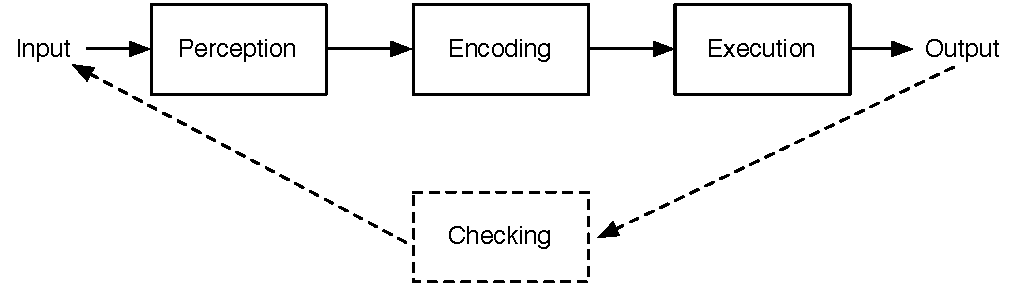
\includegraphics[width=0.8\textwidth]{images/background/HIP.pdf}
\caption[Different stages of a data entry task]{The different stages of a routine data entry task: a user perceives data input, encodes these in the mind, executes certain actions to enter data and produce the output, and can check the output against the original input.}
\vspace{-3pt}
\label{fig:ch2_hip}
\end{figure}


\subsection{The perception stage}
A data entry task begins with the user looking at the data that has to be entered on a data source.  The way in which data is presented to the user affects how that data is encoded by the user in the internal mind. The stronger data is encoded in memory, the more robust the user is against interruptions, and the less often the user may have to interrupt a task to look back at information. Several studies have shown that making information more difficult to perceive can encourage a deeper encoding in memory \citep{Diemand-Yauman2011, Soboczenski2013}. \citet{Soboczenski2013} conducted two experiments where people had to transcribe text and numbers that were presented either in a black font colour or a harder-to-read grey font colour. A hard-to-read font forced people to make more of an effort to read and understand the text, and as a result the text was more deeply processed and encoded in the mind. Participants made fewer data transcription errors if data was shown in the harder-to-read font colour, both for transcribing text and numbers. There was no difference in speed between the hard-to-read and normal font colour, suggesting that the improved accuracy was not due to a speed-accuracy trade-off. 

The way in which data is perceived and encoded is further influenced by how it is situated in the environment. The distributed cognition approach has been used as a theoretical framework to explain how cognition is ‘distributed’, meaning that people use a combination of internal information in their mind, and external information in the physical environment, to carry out work \citep{Hollan2000, Hutchins1995}. This means that to be able to understand how people work, it is not enough to know how the mind processes information, but it is also important to know how task information is situated in the physical world \citep{Hollan2000}. In most data entry studies, the data to enter is given to participants, which might not reflect how data entry is situated in offices. This motivates the need to understand how information for data entry work is spread in an office environment, which is the focus of the next chapter in this thesis. 

%\subsubsection{Summary}
%The first part of the data entry task entails the user perceiving the input.  A stronger representation of data in memory can improve task performance. Data may be strongly presented in memory because the data to enter is familiar to the user, but the design of the input source can also influence people's cognitive strategies and encourage a deeper encoding. Both internal and external information affect task performance, and where and how input is presented in the external environment affects people's internal representation of it. 

\subsection{The encoding stage}\label{sec:Encoding_stage}
After the user has perceived the input source in a data entry task, the next stage in the task sequence is the encoding stage, where data is encoded in memory. Prior work has shown several benefits of a deep encoding in memory: it can reduce interruptions to look back at information, but can also make people more robust against other, task-irrelevant, interruptions. As discussed earlier, another factor that  influences encoding is the costs associated with accessing data in the task environment. If information access costs increase, people rely on information in memory to avoid incurring costs to avoid making switches to the information source. \citet{Morgan2009} showed that in a copying task, if IAC was increased, participants made more of an effort to memorise the information. After an interruption, they were quicker to resume the task, because the pattern was still in memory. 

It is not just the external representation that influences how strongly something is encoded: in certain settings, certain data items are often re-used and thus are more strongly represented in memory. From text entry literature, it is known that words are easier to transcribe than non-words as they are used more often, they are more meaningful and thus have a stronger representation in memory \citep{Salthouse1986}. This highlights the importance to get a thorough understanding of the setting in which data entry is conducted. For example, \citet{Wiseman2013a} looked at number entry in hospitals and found some numbers were used far more often than others. Experiments showed that familiar numbers are faster to transcribe, suggesting that these are more strongly represented in memory than random numbers as well \citep{Wiseman2014} . This means that data entry interfaces that are intended for specific settings should be evaluated with familiar numbers used in that setting, rather than random numbers, and make it easier to enter commonly used numbers. 

%\subsubsection{Summary}
%At the second stage of the data entry task, the user processes the input in the mind. While usually designers aim to make it easy for people and not put too much cognitive load on the user, in some cases making the user process the information more deeply and adopt a memory-intensive strategy can have a positive effect on task performance. In the case of an interruption, taking time to remember where people were in the task sequence can reduce resumption errors. Furthermore, a deep encoding of data in memory can make people more accurate in data entry.

\subsection{The execution stage}
The third stage of the data entry task is the execution stage, which is the stage where the user performs the motoric actions to enter data into a device.

The design of the input method influences the speed with which users enter data, which can subsequently affect errors. \citet{Oladimeji2011} compared a number keypad with an incremental interface. The two types of interfaces are shown in Figure \ref{fig:interface-styles}. The number keypad is most common, and is used on calculators and phones. In this interface, each digit is assigned a button and additional buttons are usually a decimal point and a delete key to correct an error, as shown in Figure \ref{fig:numberpad}. In an incremental interface, a number is entered by increasing or decreasing the number using up and down keys. The incremental interface used in \citeauthor{Oladimeji2011}'s study is shown in Figure \ref{fig:incremental}. The double arrows increase and decrease the number by a larger amount than the single arrows. 

Results of the study showed that a number keypad allowed people to enter a number more quickly than an incremental interface, but more errors were made. With the keypad, the visual attention was more on the input keys than the display. In an incremental interface, people were changing an existing value rather than entering a new value, so they had to look at the display to see how their actions changed the current value. This attention on the display may have made it more likely for them to detect errors in time. While an incremental interface may not be feasible when entering large amounts of data as it will slow users down too much, it may be preferrable over a keypad in situations where accuracy is of great importance \citep{Thimbleby2011}. 

\begin{figure}[]
\begin{center}

\begin{subfigure}[b]{0.3\textwidth}
\centerline{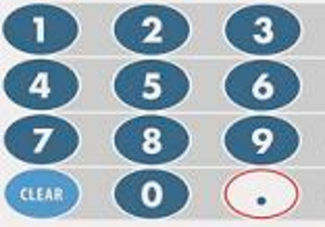
\includegraphics[scale=0.8]{images/background/numberpad.pdf}}
\caption{A number pad.}
\label{fig:numberpad}
\end{subfigure}
%\hfill%
\begin{subfigure}[b]{0.5\textwidth}
\centerline{
\includegraphics[scale=0.5]{images/background/incremental.pdf}}
\caption{An incremental interface.}
\label{fig:incremental}
\end{subfigure}

\caption[An incremental and keypad number entry interface.]{Two different number entry interfaces tested in \citeauthor{Oladimeji2011}'s study.}

\label{fig:interface-styles}
\end{center}
\end{figure}

%\subsubsection{Summary}
%At the third stage of the data entry task, the user inputs the data into a device. Data entry has a speed-accuracy tradeoff, and being able to enter data faster often come at the cost of an increased error rate. 
%Keyboards that slow people down may be useful in cases where accuracy is important, but may not be feasible in situations where a lot of data has to be entered. Depending on what users have to enter, shortcuts may get introduced in keyboard design so commonly used data can be entered quicker without the cost of increased errors. 

\subsection{The checking stage}
Most data transcription models consider the execution stage as the final stage of a data entry task \citep{Card1983, Salthouse1986}, but an additional stage can be a checking stage, where people review what they have entered and compare it with the original input, to see if it is correct. A reason why most models do not include this stage may be that people often do not make the effort to do so, and if they do, they are poor at detecting errors \citep{Olsen2008}. \citet{Olsen2008} conducted a lab experiment in which he simulated an internet banking tool, and participants were asked to enter account numbers from a paper sheet into a computer. After participants had entered an account number, they were presented with a confirmation screen with the input, and users were asked to check their input on this screen before submitting.  Participants confirmed 88 trials where they had entered an incorrect account number. In addition, in 178 trials the simulator changed people's input to another number and this incorrect number was presented on the confirmation screen. Only 5 of these 178 errors were detected and corrected. This large amount of incorrect confirmations again suggests users do not check properly, even if they are explicitly asked to do so. People are even worse at checking their input if they are switching between a data entry task and another task \citep{Wiseman2015}.

Given the limited effectiveness of confirmation screens \citep{Norman2002, Olsen2008}, some studies have supplemented these with lockouts, where users have to wait a short period of time before they are able to confirm and submit their input. While this has been shown to reduce errors in a controlled setting \citep{Gould2016b}, the presence of other tasks and distractions can entice users to switch to something else instead \citep{Gould2016b, Katidioti2013}.

\citet{Gould2016b} studied a number entry task where after each number the submit button would be disabled for a number of seconds, and a text instruction to check input appeared on the input screen.  This lockout was an effective method in encouraging people to check and detect errors in a lab setting. When the study was replicated online, a short lockout made people detect errors as well but the longer the lockout duration was, the more likely people were to switch to doing other tasks, and not check anymore. This illustrates the importance of taking the task context into account, and suggests that findings from controlled studies do not always directly translate to an applied setting \citep{Gould2016b}. 

Similar switching behaviour was found by \citet{Katidioti2013}. They conducted a lab experiment where people had to copy information and were interrupted by chat messages. Participants were free to choose when they wanted to attend to the messages. When people were locked out in the copying task and had to wait 3 seconds before they could enter the information, they often switched to the chat message, which made them forget the information to copy and slowed them down in completing the task.

%\subsubsection{Summary}
%After people have entered input, they can choose to check if what they have entered is correct. A popular method is visual checking, but people are poor at doing this, even if they are instructed to do so. It is possible to have people check, but the context needs to be considered. A lockout helped people check, but when possible to switch to other tasks people used the time to spend time on other tasks.

\subsection{Summary}
Research has shown how the way data is perceived, encoded, entered and checked all influence data entry performance. Time costs associated with perceiving data can improve encoding, and a better encoding leads to faster and more accurate entry.  The majority of data entry design interventions have been evaluated through laboratory experiments, and attempts to study data entry in a multitask setting suggest that people may interact with these interventions differently beyond a controlled setting. For example, in experimental studies the information was given and people were focused on the task, whereas many office settings are fragmented, and people can get distracted. How is data entry situated in an office setting? Are people focused on the task? And do they have the information readily available, or is this fragmented? In order to understand how people can be supported in making inquiries for data entry, it is important to understand how information for data entry is distributed in the environment.

\section{Conclusion}
This chapter reviewed literature on interruptions, information seeking and data entry. From this review, we learn that the length and timing affects the disruptiveness of interruptions, and that people try to avoid time costs in a controlled setting. As task-irrelevant interruptions are considered more disruptive than task-relevant interruptions, interruption management tools have mostly focused on avoiding these, even though relevant interruptions can be just as disruptive if not managed well. Furthermore, based on prior literature on information management we learn that how people search for information depends on the type of work. While existing tools support tasks where information sources need to be re-used, these provide no guidance of how to interrupt a task to collect information in the first place. Lastly, data entry research has shown that design interventions can reduce data entry errors if people are focused on the task, but that the context needs to be considered: people have workarounds to these design interventions if they (have to) interrupt and are exposed to distractions.

This highlights a need to better understand inquiries for a data entry task, and how the disruptiveness of these inquiries can be reduced. The next three chapters report a series of studies aimed to understand how interruption management tools can support people in managing inquiries for a routine data entry task, given variable time costs of required inquiries. To design a suitable tool, an understanding is required of how people currently self-interrupt for data entry work, which will be the focus of the next chapter.

%Based on prior work reviewed in this chapter, I make the hypothesis that disruptiveness can be reduced by reducing the length and number of interruptions, and by making interruptions at low workload moments in the task. I also make the hypothesis that people try to minimise time and that 

%Data entry follows four stages, and there are multiple strategies to complete the task, some being more accurate or efficient than others. Studies have shown that changing the design of a data entry interface can affect and improve how we enter data, and that different information access costs affect how often people visit the source from which to look up and enter data.

%It is not known yet how these data entry designs can be used in an office setting, where people have to manage multiple information sources with varying information access costs. Studies on office work have shown that work can be highly fragmented, and that people may often have to go in and out of several applications to complete their task. 
%In order to design interactive systems that truly support this type of data entry task, it is necessary to get a detailed understanding of the task in this setting, how users manage subtasks of looking up information for the data entry task, and to what extent the costs to access required resources affect their strategies. %Literature review
%All chapters go here
\chapter{Entering expenses in a financial setting}\label{ch:Study1}
\begin{mynote}
\subsubsection{Chapter outline}

In this chapter I describe the findings of an explorative interview study about data entry in a financial work setting. The aim of this study was to get a better understanding of the type of data entry task people at finance offices conduct, and the physical environment in which this is done.
A second planned study is described, that aims to investigate the information sources finance office workers need for an expenses task, and how they currently manage subtasks of looking up information.

\end{mynote}

\section{Study 1: Understanding data entry work in a financial office}\label{ch:Study1}
 
\subsection{Introduction}
As data entry is a common task and it is important this is done both accurately and efficiently, work has been done to design and optimise data entry interfaces to support fast and accurate data entry \citep[e.g.][]{Oladimeji2013, Vertanen2015, Wiseman2013a}.
However, it is not just the input method that determines efficiency and accuracy but also other aspects of the task, such as the environment within which it is conducted \citep{Payne2013, Randall2014}.

\citet{Evans2012} looked if people's text entry and mouse pointing behaviour in a lab setting was comparable to how they would normally perform these inputting tasks in their everyday life. They remotely observed people's input behaviour on their personal computer, and compared this with their performance on similar tasks in a lab. Participants installed a tool on their personal computer which logged all text entry and mouse pointing behaviour they performed in one workweek. Examples of tasks that were carried out were sending personal messages to friends and browsing the web. There were no differences in uncorrected errors or text entry speed between the lab and the field, but they did find that participants corrected more errors in the lab. This study shows that people check and correct their entries more when they are in a controlled environment and are focused on the task, though the measured behaviour on people's personal computers mostly included tasks where accuracy may not have been considered important, such as sending an informal chat message to a friend. 

In order to support people in their data entry work, it is important to first have a better understanding of the types of data entry tasks they have to conduct, and the physical environment in which this is done. Therefore, the first study of this thesis is an explorative study. I visited and interviewed people who conduct data entry tasks as part of their daily work in the finance departments of two universities. This user group was chosen as they have a lot of data entry tasks as part of their job, and it is an area where it is important to enter data accurately, but there is also time pressure to finish work on time. Furthermore, it was an accessible user group to approach for the researcher.

Previous research has given us a good understanding of which factors may influence people's performance on a data entry task. The current study aims to study how these factors are laid out in an applied setting. Furthermore, this study gives an opportunity to see if there are additional problems that influence data entry performance, that are currently not acknowledged in existing literature. 

\subsection{Method}
\subsubsection{Participants}
Nine participants (four male) took part in the study. They were employees from two public universities and their work involved receiving various requests for payment, checking the information of these requests was correct, and entering the information along with administration data into computer systems. Ages ranged from 18 to 52 (two participants wished to not disclose their age). Their level of experience differed, with some participants having just started doing this type of job and other participants working in Finance for 17 years. All but one worked full-time. Table \ref{table:ch3_participants} shows further demographic details of the participants. Typical tasks participants dealt with were checking and entering expense forms sent by staff and students, paying salaries and pensions, controlling research budgets, monitoring university income and expenses and entering employee information. Participants were recruited by sending invitations to opt-in mailing lists of Finance departments, and were reimbursed with a \pounds10 Amazon voucher.

\begin{table}[htp]
\centering
\resizebox{\textwidth}{!}{%
\begin{tabular}{llllllll}
{\bf ID} & {\bf Age} & {\bf Gender} & {\bf Nationality} & {\bf Occupation}                                                             & {\bf University} & {\bf \begin{tabular}[c]{@{}l@{}}Experience in\\ Finance\\ (y = years,\\ m = months)\end{tabular}} & {\bf Deals with}                                                                                     \\ \hline
P1       & 49        & M            & Danish            & \begin{tabular}[c]{@{}l@{}}Research\\ Services\\ Administration\end{tabular} & A                & 17y                                                                                               & \begin{tabular}[c]{@{}l@{}}invoices,\\ statements,\\ grants\end{tabular}                             \\
P2       & 39        & F            & British           & Administrator                                                                & A                & 2y                                                                                                & \begin{tabular}[c]{@{}l@{}}funding,\\ expenses,\\ room\\ bookings,\\ events\end{tabular}             \\
P3       & 20        & F            & British           & \begin{tabular}[c]{@{}l@{}}Credit\\ Controller\end{tabular}                  & A                & 7m                                                                                                & \begin{tabular}[c]{@{}l@{}}money that\\ comes in,\\ payments\end{tabular}                            \\
P4       & -         & M            & British           & \begin{tabular}[c]{@{}l@{}}Assistant\\ Accountant\end{tabular}               & A                & 15y                                                                                               & \begin{tabular}[c]{@{}l@{}}research\\ budgets,\\ expenses\end{tabular}                               \\
P5       & 33        & F            & British           & \begin{tabular}[c]{@{}l@{}}Accounts\\ Assistant\\ Expenses\end{tabular}      & A                & 4y2m                                                                                              & \begin{tabular}[c]{@{}l@{}}expenses,\\ employee\\ information,\\ supplier\\ information\end{tabular} \\
P6       & 18        & M            & British           & \begin{tabular}[c]{@{}l@{}}Payroll and\\ Pensions\\ Apprentice\end{tabular}  & B                & 6m                                                                                                & \begin{tabular}[c]{@{}l@{}}salaries,\\ expenses,\\ pensions\end{tabular}                             \\
P7       & 40        & F            & British           & \begin{tabular}[c]{@{}l@{}}Payroll and\\ Pensions\\ Assistant\end{tabular}   & B                & 10y                                                                                               & \begin{tabular}[c]{@{}l@{}}salaries,\\ expenses,\\ pensions\end{tabular}                             \\
P8       & 52        & M            & British           & \begin{tabular}[c]{@{}l@{}}Payroll\\ Supervisor\end{tabular}                 & B                & 12y                                                                                               & \begin{tabular}[c]{@{}l@{}}salaries,\\ expenses,\\ pensions\end{tabular}                             \\
P9       & -         & F            & British           & Payroll Officer                                                              & B                & 13y                                                                                               & \begin{tabular}[c]{@{}l@{}}salaries,\\ expenses,\\ pensions,\\ employee \\ information\end{tabular} 
\end{tabular}
}
\caption[Study 1 participant information]{Participant information.}
\label{table:ch3_participants}
\end{table}

\subsubsection{Materials}
Materials that were used during the interview were a voice recorder, a paper copy of an interview script with the interview topics and guiding questions, a consent form, an information sheet for the participant and a notebook and pen to make notes. The interview script, information sheet and consent form are included in the Appendix. 
Each interview covered four guiding topics, which are briefly described in Table \ref{table:ch3_interviewtopics}. For each topic, a number of questions were written out beforehand. These questions were used as a starting point to get the participant talking and guide the interview. Based on what the participant was saying follow-up questions were asked. The audio transcription program ExpressScribe was used to transcribe the interviews. The data analysis programs Nvivo and Atlas.ti were used to analyse the data. Nvivo was used to code the interview transcripts and notes. Atlas.ti was used to complement the analysis in Nvivo and allowed to identify relations between codes.

\begin{table}[htp]
\centering
    \begin{tabular}{ | l | p{10cm} |}
    \hline
     Topic & Description \\ \hline
    Job description & A description of the tasks that the interviewee deals with. The purpose of this topic was to start the interview easy and give the interviewee the opportunity to explain what their job entails. \\ \hline
    Number transcription & This includes questions on when and how people typically enter numbers for work.  \\ \hline
Environment & This topic includes people's physical work environment, and the organisation they are a part of. \\ \hline
Demonstration &  Interviewees were asked to give a demonstration of entering data into their system. The aim of this part of the interview is to see the type of data entry tasks people have to do, and also gives a chance to see the information sources and systems people currently use. \\
    \hline
    \end{tabular}
    \caption[Study 1 interview topics]{Interview topics.}
    \label{table:ch3_interviewtopics}
\end{table}%

\subsubsection{Data recording}
A voice recorder was used to audio record the interviews. One participant wished to not be audio recorded and one interview could not be audio recorded due to technical issues, so for these two interviews notes were taken of the answers. For the remaining seven interviews, notes were only made of observations and not the participants' answers. Notes were made with pen and paper. Photographs were made of the work environment and screenshots of the systems that the interviewees used.

\subsubsection{Interviewing procedure}
The interviews took place at the participants' workplace. For two interviews, the interviewee's office place was not suitable for talking so the interview took place in a common room nearby, and these participants showed their workplace and completed a demonstration of entering data after the interview. 
Participants were welcomed and informed about the study. They received a paper information sheet with the outline of the study and contact details of the researcher to keep for future reference. They were also asked to read and sign a consent form.

The interviews were semi-structured and took between 20 and 55 minutes. Each interview was reviewed afterwards, and findings sometimes fed into new questions being included or some questions being adapted in subsequent interviews.

\subsubsection{Pilot interview}
A pilot interview was conducted with an acquaintance of the researcher who worked in Finance, to test out the set-up of the study and questions. The interview took place at the participant's home, notes were taken with pen and paper, and the interview was audio-recorded using iMovie on a Macbook Pro. 

Taking notes slowed down the flow of the interview: sometimes the interviewee stopped talking to give the interviewer the opportunity to finish taking notes. Furthermore, taking notes took attention away from what the interviewee was explaining: assumptions made during the interview did not seem to be accurate in later analysis. Therefore, it was decided that note taking would be kept to a minimum. Notes would only be made of observations that could not be taken from audio recordings.

The interviewee talked elaborately about manually converting different currencies, and identified this task as the main place where errors occurred. Therefore, questions were included about if interviewees dealt with foreign currencies and converting these. 

\subsubsection{Ethical considerations}
The study was undertaken with ethical approval from the UCL Research Ethics Committee [Project ID Number UCLIC/1415/001/Staff Brumby/Borghouts]. 
At the start of each interview, participants were first informed verbally about the study. They were then given a consent form to read and sign, and were given an information sheet to keep. This information sheet contained the study information and contact details of the researcher and the project's principal researcher, should participants have any further questions after completion of the study.  They were asked permission for the interview to be audio recorded. One participant wished not to be audio recorded and notes were taken instead. 

Participants were informed that the data would be used for research purposes only and stored in accordance with the Data Protection Act 1998. They were also informed that their data would be anonymised and when used in a report or academic paper, their data would not be directly identifiable. Names of participants or the universities they were working at were not included in the interview notes and transcripts.
 
\subsection{Results}
\subsubsection{Data analysis}
After each interview or set of interviews, a first analysis took place. The audio recording was played back, notes were typed into a digital file and reviewed and the interview was transcribed verbatim. Several non-verbal cues were included in the transcription as well, such as when the interviewee laughed or sighed, as well as descriptions of when the interviewee was demonstrating something. The advantage of doing the transcription shortly after the interview was that it was still easy to remember from listening to the audio recording what was being demonstrated. Interesting findings and initial patterns that were apparent across the data were written down. 

After all interviews had been transcribed, the transcriptions and notes were printed and the data was analysed using thematic analysis \citep{Braun2006}. Anything in the data that was considered to be interesting was annotated by hand and labelled with an appropriate code. On reviewing the coding, some codes were grouped together in one code, additional codes were named, and similar codes were grouped under themes. For instance, an initial code was Notifications, such as e-mail notifications. During the second coding iteration, it was identified that people always talked about notifications in the context that they were interrupted (by a notification) rather than about notifications on its own. Therefore, notifications and interruptions were grouped into one code. 

The themes were then reviewed, to see if they addressed the purpose of the study. The transcripts and notes were then imported into Nvivo and coded digitally. Atlas.ti was used to complement this analysis and allowed to identify relations between codes. 

\subsubsection{Themes}
In total 51 codes were derived, and these were grouped into 8 main themes, which are listed and described in Table \ref{table:ch3_themes}. If codes or separate quotes did not belong in a certain theme but were still considered relevant, they were grouped in the Other category. 

\begin{table}[htp]
\centering
\resizebox{\textwidth}{!}{
    \begin{tabular}{ | p{3cm} | p{8cm} | l | l |}
    \hline
     \textbf{Theme} & \textbf{Description} & \textbf{Quotations} & \textbf{Participants} \\ \hline
     Task characteristics & People described things that were particular to their task, for instance how they structured their task, whether they switched tasks, and how long they took to complete tasks.  & 129 & 9 \\ \hline
	 Checking & People talked about checking data input as part of their job. & 103 & 9 \\ \hline 
	System & People talked about the computer system they were using to input data.  & 91 & 9 \\ \hline 
		Environment &People described their environment, for instance they talked about their physical work setting, and the work culture of their organisation. & 80 & 9 \\ \hline 
		Data &People described the data they were dealing with, for instance the type and length of data items, and from which source they copied data. & 75 & 9 \\ \hline 
		Errors &People described situations where errors were made: who made them, why were they made, what were the consequences. & 75 & 9 \\ \hline 
					 Strategy & People described the strategies they used to carry out their task.  & 54 & 9 \\ \hline 
		Importance of accuracy and paper trails &People talked about the sensitivity of financial data which is why not all people are authorised to approve or access financial data, and the importance of a paper trail for data entries. & 35 & 8 \\ \hline 
			 			 Other & People talked about things that did not fit into any other category but were still considered relevant, such as issues they experienced, or queries they often received.   & 74 & 9 \\ 
    \hline
    \end{tabular}
    }
    \caption[Study 1 Themes]{The themes, along with a description. The column Quotations indicates how many times this theme was brought up during interviews, and the column Participants indicates how many participants talked about it.}
    \label{table:ch3_themes}
\end{table}

Each theme is described separately in subsections below, and is visualised in a diagram, which shows the theme's main codes and relationships between codes, as well as quotes in dotted squares to exemplify what type of quotes were grouped under this code. The numbers in parentheses indicate the number of quotes, and the number of interviewees who mentioned it. 
The description of each theme is accompanied with notes and quotes taken from the transcripts to further illustrate when this theme was mentioned. These serve as examples and are not all the instances of a theme. To differentiate notes from verbatim quotes, the quotes are in italics and double quotation marks. Words put in brackets are added by the researcher to make the quote more understandable for the reader, for instance if the interviewee is talking about 'it' or 'them'.
The results are ordered according to the number of quotations associated with a theme, with the theme with the most quotations listed first. The only exception is the 'Other' theme which is described last.
\newpage
\subsubsection{Task}
\begin{figure}[!ht]
\centering
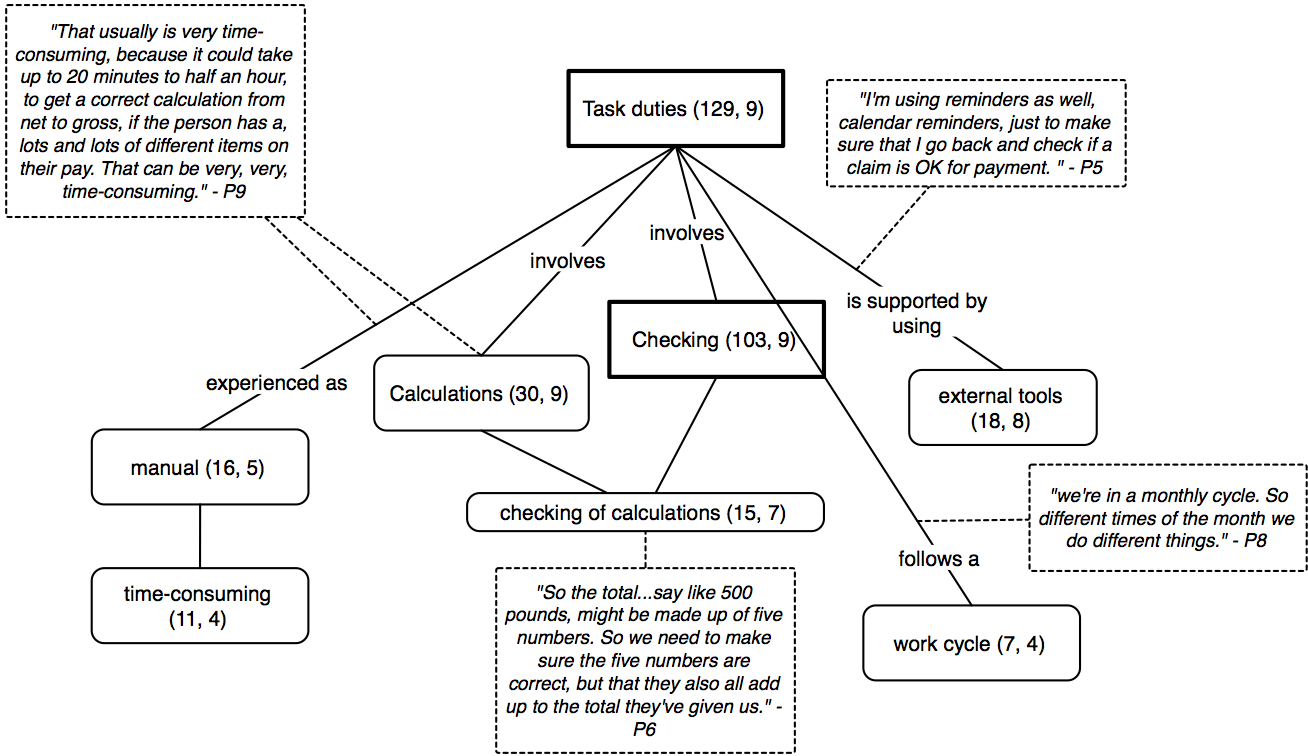
\includegraphics[width=\textwidth]{images/Study1/Task.png}
\caption[Study 1 Task diagram]{Diagram showing the theme Task. The numbers in parentheses indicate the number of quotes and the number of participants who mentioned it, respectively.}
\vspace{-9pt}
\label{fig:ch3_task}
\end{figure}
A common data entry task was entering expenses. Interviewees received expense claims from students and staff and had to check the information was correct. They then had to enter this data, along with other information such as budgetting and staff information, into a computer system.
All interviewees mentioned a large part of their job was checking that data was correct. In addition to transcribing and checking individual numbers, participants also mentioned they often have to perform and check calculations.
 Some tasks, such as calculations, had to be done manually and this was described as time-consuming. People used several external tools in their environment to support them in their tasks. For instance, P7 and P8 had paper sheets on their desk with information they frequently had to look up, so they could easily use this to check if the input they had received was correct.

Some people worked according to a work cycle, which meant they did different things at different times of the month. One week could be reserved for checking all the data they received from another department, while another week could be spent on solely inputting data. 

The time spent on each task differed: checking data on a short expenses form could be completed in two minutes, while a single calculation could take between 20 and 30 minutes. Two participants experienced dealing with a lot of data entry as tiresome.

\newpage

\subsubsection{Checking}\label{subsec:Checking}
\begin{figure}[!ht]
\centering
\includegraphics[width=\textwidth]{images/Study1/Checking.pdf}
\caption[Study 1 Checking diagram]{Diagram showing the theme Checking.}
\vspace{-9pt}
\label{fig:ch3_checking}
\end{figure}

All participants talked about checking data input for errors as a part of their job. Data was checked by several different people and departments before it was submitted. People's experience with this checking system differed: P3 felt that an error would be caught eventually because it goes through so many different layers, whereas P9 said it made people less careful about making errors and therefore they often received erroneous data. Sending wrong input back slowed the process down, and P8, who acted as the last person in his department to check before it gets submitted, warned that even with extra human checks not all errors get caught. 

People had to both check their own data input, as well as double-check other people's input. They maintained different checking strategies, ranging from checking each data item one by one to entering a group of data items first and then checking. 


\begin{table}[htp]
\centering
    \begin{tabular}{ | l | p{10cm} |}
    \hline
     \textbf{Participant} & \textbf{Quote} \\ \hline
    P3 & \textit{"we try and pick it [errors] up and then obviously there's all the different stages that pick it up as you go along."}\\ \hline
    P9 & \textit{"the departments actually sometimes treat us as a checking system [laughs], but they shouldn't really, the schools. Because we're here just to make sure that people get paid correctly. But even though we are like a second check, we feel sometimes that we are the first checkpoint."} \\ \hline
    P7 & \textit{"All this piece of work, when we input in the system, will be actually checked by another person... my manager will print it out, and then check... other colleagues will double-check it for you as well, the calculations."} \\ \hline
    P8 & \textit{"one of these errors could be things that are missed during the checking."} \\ \hline

    \hline
    \end{tabular}
    \caption[Study 1 checking quotes]{Verbatim quotes taken from the interview transcripts that were about checking.}
    \label{table:ch3_checkingquotes}
\end{table}%

\begin{table}[htp]
\centering
    \begin{tabular}{ | l | p{10cm} |}
    \hline
     \textbf{Participant} & \textbf{Quote/note} \\ \hline
    P1 &  first puts in all the details, then when done checks everything against the source. \\ \hline
    P7 & when entering numbers from paper to computer, mostly looked at paper form and the number pad; only looked at screen after finishing entering all the numbers from the form to check. \\ \hline
    P5 & \textit{"We would go by the receipt, so we would try to make sure that the receipts are in order."} \\ \hline

    \hline
    \end{tabular}
    \caption[Study 1 checking own input]{Checking own input when entering data.}
    \label{table:ch3_owninputquotes}
\end{table}%

\begin{table}[htp]
\centering
    \begin{tabular}{ | l | p{10cm} |}
    \hline
     \textbf{Participant} & \textbf{Quote} \\ \hline
    P5 &  \textit{"The numbers on the expense form will be checked individually. So the total will obviously be, say like 500 pounds, might be made up of five numbers. So we need to make sure the five numbers are correct, but that they also all add up to the total they've given us."} \\ \hline
    P6 & \textit{"The numbers on the expense form will be checked individually."}\\ \hline
    P9 & \textit{"We have to check it one by one."} \\ \hline

    \hline
    \end{tabular}
    \caption[Study 1 checking other people's input]{Checking other people's input.}
    \label{table:ch3_otherinputquotes}
\end{table}%

\clearpage
\subsubsection{System}
\begin{figure}[!ht]
\centering
\includegraphics[width=\textwidth]{images/Study1/System.pdf}
\caption[Study 1 System diagram]{Diagram showing the theme System.}
\vspace{-9pt}
\label{fig:ch3_system}
\end{figure}

Data had to be entered into an information system on a computer. Some participants mentioned the system was another way to check for erroneous data entries: if the allowed number range of a variable was known, the system would let the user know if an out-of-range number was entered. However, it was also mentioned that one issue with the financial data entry system was that it did not give feedback if there was an issue or error.

The information needed for one task was usually spread over several windows on the computer, so sometimes people had to flick back and forth or memorise certain information from one window to use in another window. 

\clearpage
\subsubsection{Environment}
\begin{figure}[!ht]
\centering
\includegraphics[width=\textwidth]{images/Study1/Environment.pdf}
\caption[Study 1 Environment diagram]{Diagram showing the theme Environment.}
\vspace{-9pt}
\label{fig:ch3_environment}
\end{figure}

Every time people described the environment they were working in, this was grouped under the Environment theme. The environment could be their immediate physical setting, or their organisation in general. 

All participants experienced interruptions during work. P8 mentioned he had to pause his task immediately if a staff member needed his help, but considered these interruptions part of his job. Other interviewees mentioned they tried to concentrate on the task at hand first, but did briefly attend to interruptions such as e-mail notifications, in case it was important.

People were dependent on other departments to finish a task. For instance, P5 checked paper expense forms, but did not enter these into the system herself. 

Some participants felt the pressure to be both accurate in data entry, as well as finish it quickly because of deadlines. The workload varied throughout the year.

\newpage
\subsubsection{Data}
\begin{figure}[!ht]
\centering
\includegraphics[width=\textwidth]{images/Study1/Data.pdf}
\caption[Study 1 Data diagram]{Diagram showing the theme Data.}
\vspace{-9pt}
\label{fig:ch3_data}
\end{figure}

Participants had to retrieve data from various sources. Some of the sources were electronic, such as Excel spreadsheets and Word documents. Some information had to be looked up in databases and work e-mails. Other information was received on paper sheets, and some participants had printed out information they frequently needed and had placed this on their desk. People had to transcribe numbers from paper onto a computer system for at least a part of their tasks. Some people worked with two screens.
The amount of data that people dealt with differed. P5 said that for expenses alone, the amount of numbers she received each day to check and input ranges from 100 to 6000 numbers.
People primarily dealt with numeric data, such as financial data and IDs. The monetary numbers they dealt with ranged from five to millions of pounds. Participants also entered and checked alphanumeric and non-numeric data such as employee names, addresses and bank account details.

Numeric data consisted of individual numbers, as well as groups of numbers that together made up a new number, such as the total amount of money spent on a project. Participants had to both check and transcribe each individual number, and check that the calculation was correct. 

\ \clearpage

\subsubsection{Errors}
\begin{figure}[!ht]
\centering
\includegraphics[width=\textwidth]{images/Study1/Errors.pdf}
\caption[Study 1 Errors diagram]{Diagram showing the theme Errors.}
\vspace{-9pt}
\label{fig:ch3_errors}
\end{figure}

Participants discussed that errors happened frequently, and talked about errors they spotted from other people. Visual checking was mentioned as the main method to catch and correct errors in time, but when possible the computer system sometimes checked for erroneous data as well. Errors that were made were typos, miscalculations, or people had the wrong information to enter. For instance, P7 mentioned that when salary rates change, employees often keep entering their old salary rate on claim forms, which then has to be corrected. The main explanation people gave for errors was that it is human to make mistakes, but it was also mentioned people are under time pressure, and that people rely on the fact it will be checked by another person, which makes them less careful in entering accurate data. 
If an error was spotted, this had certain consequences depending on if the error was acceptable or not. If the error was sufficiently small, it could be either processed or corrected without negotiation, but if it was a large error, it had to be sent back or forwarded to a higher authority for approval. 

P1 highlighted project IDs used to be letters but are now numbers, which are harder to memorise, and he felt it was easier to make a mistake. P4 worked with both paper and digital files to transcribe data from, but preferred digital files because he felt it was much easier to make an error and omit figures when transcribing from paper.

\begin{table}[htp]
\centering
    \begin{tabular}{ | l | p{10cm} |}
    \hline
     \textbf{Participant} & \textbf{Quote/note} \\ \hline
    P6 &  \textit{"it's quite common that we have to return an expense or payment back to someone. It happens quite often, yeah."} \\ \hline
    P4 & Yes all the time, lots of typos.\\ 
    \hline
    \end{tabular}
    \caption[Study 1 errors quotes]{People mentioned errors occur quite frequently.}
    \label{table:ch3_occurrenceerrorsquotes}
\end{table}%


\begin{table}[htp]
\centering
    \begin{tabular}{ | l | p{10cm} |}
    \hline
     \textbf{Participant} & \textbf{Quote} \\ \hline
    P3 &  \textit{"sometimes it's because people have done typos, done too many zeroes, or left out a zero."} \\ \hline
    P5 & \textit{"the expense breakdown doesn't match what (...) whatever they put as the grand total."}\\ 
    \hline
    \end{tabular}
    \caption[Study 1 type of errors quotes]{The type of errors.}
    \label{table:ch3_typeoferrorsquotes}
\end{table}%


\begin{table}[htp]
\centering
    \begin{tabular}{ | l | p{10cm} |}
    \hline
     \textbf{Participant} & \textbf{Quote} \\ \hline
    P9 &  \textit{"Because the departments actually sometimes treat us as a checking system [laughs], but they shouldn't really."} \\ \hline
    P7 & \textit{"Yeah, human laziness or something [laughs]."}\\ \hline
    P8 & \textit{"sometimes, you know, through human error, you know, things don't get paid properly."} \\
    \hline
    \end{tabular}
    \caption[Study 1 reasons for errors quotes]{The reasons for errors.}
    \label{table:ch3_errorreasonsquotes}
\end{table}%


\begin{table}[htp]
\centering
    \begin{tabular}{ | l | p{10cm} |}
    \hline
     \textbf{Participant} & \textbf{Quote/note} \\ \hline
    P5 &  \textit{"generally we tend, we try not to send claims back to departments because they might get lost in the post, and it's an inconvenience as well. So we try to... resolve it ourselves.."} \\ \hline
    P4 & We allow a certain amount of tolerance; if it turns out the thing you bought has actually decreased value and is now  \pounds40, we will allow to return  \pounds50\\ \hline
    P7 & \textit{"we normally e-mail the budget holder to say... what you authorised is actually different. But for this kind of thing, it's only 10 pounds...we normally just process this without contacting them."} \\ \hline

    \hline
    \end{tabular}
    \caption[Study 1 acceptable errors quotes]{Acceptable errors.}
    \label{table:ch3_acceptableerrorsquotes}
\end{table}%

\clearpage
\subsubsection{Strategy}
\begin{figure}[!ht]
\centering
\includegraphics[width=\textwidth]{images/Study1/Strategy.pdf}
\caption[Study 1 Strategy diagram]{Diagram showing the theme Strategy.}
\vspace{-9pt}
\label{fig:ch3_strategy}
\end{figure}

Eight of nine interviewees saved up data to enter it all in one sequence. If they received forms with data input to check or enter, they saved these for later and then processed all the forms. P1 indicated he processed forms in batches of at least five forms, and found it disruptive to do just one or two and then switch to something else. 

P2 was the only interviewee that processed forms with numbers to enter as they came in, but did admit that if she had more data to fill in, she would probably do it in a more efficient way.

Some people said they preferred batching their work so that they entered all data into a single system at once because it is quicker and easier to do the same type of tasks in one sequence, and when that is finished concentrate on another task. P4 mentioned he does them all at once because he gets the forms in a bulk and feels pressure by his boss to finish them all immediately, rather than spread them over time. P6 explained he postpones processing expense forms until the deadline to submit forms for that month has passed, after which he does all forms in one sequence. 

People also talked about other strategies they used to do their job more efficiently. For instance, if they had to get out of the system to look up information digitally and then get back to the system window to enter it, they preferred to memorise the information, rather than flick back and forth and look it up each time they needed it. With numbers they had to enter frequently such as project codes, they memorised it even if they did not deliberately choose to do so. If the information to remember was complicated, they would write it down.

As discussed at the \nameref{subsec:Checking} section, people had different checking strategies and the number of times they looked back to the data source to check it against the data input varied. P7 said she sometimes deals with similar calculations, so she prefers to check the calculation she did last time rather than calculate it again. 

People explained that a lot of numbers they enter are calculated from other numbers. Some people liked to write out and keep a record of their calculation, in case someone had any questions on how that number was calculated.

\begin{table}[htp]
\centering
    \begin{tabular}{ | l | p{10cm} |}
    \hline
     \textbf{Participant} & \textbf{Quote/note} \\ \hline
    P3 &  \textit{"I just try and do it in the quickest way...It's nice, once you've done it, it's completed, so it's sort your weight lifted [laughs]. So you don't need to think about it again."} \\ \hline
    P6 & \textit{"the expenses are done in a bulk, rather than separated over a period of time. When I'm doing it lots at a time, I think once you get into sort of the hang of it, it gets done a lot quicker than..you just get used to putting them in, and inputting it all."} \\ \hline
    P9 & \textit{"I try to concentrate on my task...I try to do one task [i.e. doing all expenses], finish one, and then do another."} \\ \hline
    P4 &  It's difficult to take rests or even switch in-between number entry tasks because of the work pressure, and feels pressure by boss. \\ 
    \hline
    \end{tabular}
    \caption[Study 1 batching quotes]{Most participants entered all numbers in one go.}
    \label{table:ch3_inonegoquotes}
\end{table}%

\begin{table}[htp]
\centering
    \begin{tabular}{ | l | p{10cm} |}
    \hline
     \textbf{Participant} & \textbf{Quote/note} \\ \hline
    P3 &  \textit{" I wouldn't necessarily have to [memorise numbers], It's more just if you have to keep flicking back to different things, it's sometimes just easier to write it down, or just try and remember it. But you can obviously take the long version and keep flicking back to the correct screen."} \\ \hline
    P2 & \textit{"we have different grants and different project codes as a result, but you, because you use them so much, you end up remembering them."} \\ \hline
    \end{tabular}
    \caption[Study 1 strategy quotes]{Examples of strategies people used.}
    \label{table:ch3_strategiesquotes}
\end{table}%

\ \clearpage

\subsubsection{Importance of accuracy and paper trails}
\begin{figure}[!ht]
\centering
\includegraphics[width=\textwidth]{images/Study1/Papertrail.pdf}
\caption[Study 1 Importance of accuracy and paper trails diagram]{Diagram showing the theme 'Importance of accuracy and paper trails'.}
\vspace{-9pt}
\label{fig:ch3_papertrail}
\end{figure}

Because interviewees were working with sensitive financial data, another theme was importance of accuracy and paper trails.
Some data could only be entered in the system and modified by certain people.
Large figures had to be approved by a superior first before it could be processed, so it was clear to an auditor that expenses were made with the correct approval.
Hard copies of data had to be archived and were checked by external auditors. For instance, all expenses were claimed on paper forms, and had to have the original receipts as evidence that the expense claims were correct. Some data could not be given over the phone but had to be written down and sent via a paper form.

\pagebreak

\subsubsection{Other}
\begin{figure}[!ht]
\centering
\includegraphics[width=\textwidth]{images/Study1/Other.pdf}
\caption[Study 1 Other diagram]{If people described issues, it usually had to do with the system.}
\vspace{-9pt}
\label{fig:ch3_other}
\end{figure}

Interviewees mentioned several issues they experienced. Most of the time, the issues had to do with the current data entry system they were using. P7 mentioned number entries on the computer screen were small and hard to read, and could not be enlarged. P5 mentioned she did not get notifications from the system if there was an issue with a payment, so she would not know about it until staff members would call up to complain they had not been paid yet.  Other issues had to do with the organisation, such as the experience that the multiple checking layers made people rely on other people to check their input.

\begin{table}[htp]
\centering
    \begin{tabular}{ | l | p{10cm} |}
    \hline
     \textbf{Participant} & \textbf{Quote/note} \\ \hline
    P5 &  \textit{"There are other issues. You could say I think hundreds, I mean not just with the work that we do on expenses, but across [university A], across [university A] Finance, the Finance division...We just have to kind of work our way around the system and you know, adapt to it."} \\ \hline
    P7 & \textit{"It's only the matter of how you get used to the Payroll system. Because companies have different systems, the data inputting can take a while to get used to it."} \\ \hline
    P9 &  \textit{"You know, all systems are a bit funny, I think. But you just gotta get used to it."} \\ \hline
    \end{tabular}
    \caption[Study 1 issues quotes]{Issues that participants experienced with the system.}
    \label{table:ch3_otherquotes}
\end{table}%

\pagebreak

\subsection{Discussion}
The purpose of this study was to gain a better understanding of the type of data entry tasks in financial offices, and the physical environment in which these are conducted. For this purpose nine interviews were conducted with staff from two public universities who worked with financial data. The main findings of the study are: 

\begin{itemize}
\item 
people have to get the data to enter from various sources, with varying information access costs
\item 
people batch their work to enter a lot of data entry at once, and minimise switching between tasks. 
\item 
data entry errors are common, and the current solution is to have data entered and checked by multiple people before it gets submitted to the system
\end{itemize}

\subsubsection{Information sources and access costs}
A prevalent data entry task of participants' work was processing expense claims from university staff and students. A substantial part of this task is not just entering the data but also collecting it from multiple sources. For example, the expenses had to be entered from paper forms and receipts, foreign currencies had to be converted and copied from a website, and staff and financial information had to be retrieved from sources such as electronic spreadsheets, databases and e-mails. 
In data entry experiments, the data is often shown on a computer, to make it easy to manipulate. This was sometimes the case in the office setting studied here, but data was also transcribed from paper sheets into a computer. Furthermore, in lab experiments people are often only presented with the data they have to enter and sometimes are given only one data item at a time. The sources from which people had to enter data in this study usually contained a lot of data, not all of which was relevant to the task. The amount of irrelevant data on the sources can increase the time people need to look up the information they need.

The cost to access the information sources differed. For instance, some paper sheets were on people's desk, but some paper sheets had to be retrieved elsewhere. Sometimes participants had to go through a large spreadsheet, before they found the number they needed to copy. Participants also dealt with multiple windows on their computer screen, and sometimes needed to switch between different windows. Instead of flicking back and forth to view information they had to enter in another window, people said they preferred to memorise it. This supports previous research which showed that people make strategic use of internal and external resources and do not always maximise off-loading cognition to external resources \citep{Gray2006}. Even though participants were aware they did not have to remember information, they found this easier and faster rather than looking it up or writing it down. 

This strategy allows people to be faster, but carries the risk that they misremember it. In previous studies, trying to hold more items in memory during a copying task increased errors \citep[e.g.][]{Morgan2009}. However, in these studies people had to copy over coloured blocks, which were abstract to the participants and may have been too hard for participants to memorise \citep{Waldron2011}. In the current study, the information had some meaning to the users, and even if they were dealing with abstract information, such as project codes or ID numbers, some items were entered more often than others. Participants mentioned that even if they did not make a conscious effort to memorise these, they had to enter these numbers so often that they ended up remembering them. This is in line with prior findings that some numbers are more familiar than others, and that these familiar numbers are more strongly represented in memory \citep{Wiseman2014}. 

If information to copy is familiar and contains numbers and text, making the effort to encode the information more deeply has been shown to make people more accurate \citep{Gray2004, Soboczenski2013}. It is therefore not clear if the effect of a memory-based strategy on accuracy, as found in \citep{Morgan2009}, would extend to copying the material of this study.

People used some external tools to aid memory. For example, some participants had printed sheets with information they used and entered often, so they did not have to repeatedly look this up in the system. They also used calculators and pen and paper to perform calculations.

\subsubsection{Batching data entry tasks}
Eight of nine participants batched data entry tasks to do them all at once, rather than spread them over time. The only participant who processed expense forms as they came in said she did not receive a large amount of forms. She explained that if she dealt with a higher volume of expenses, she would probably do it in a more efficient way.

There were different reasons behind the strategy to enter a large amount of data in one sequence. One participant received forms in a bulk, and felt time pressure to finish them all at once, rather than spread them over time. The other seven participants said they received forms on an ad-hoc basis, but deliberately saved them until a specific moment and then processed them all in a bulk. They preferred to focus on one task at once, and some people stated that it made them faster in entering data after a while. 

This is consistent with Healy et al.'s \citeyearpar{Healy2004} study, where learning effects could be measured in a number entry task. However, in their experiment participants became faster but also more erroneous in entering data. In the current study, P3 mentioned that most of the errors she picks up from colleagues are typos caused by rushing to finish the task. P4 mentioned that he wants to enter numbers accurately, but that there is a time pressure to finish things in time. This is in line with the speed-accuracy trade-off discussed in literature, and that a sense of urgency may cause people to enter numbers faster but at the expense of a higher error rate \citep{Lin2011, Lin2013}.
\citet{Healy2004} recommended regular breaks when entering large amounts of data to maintain accuracy, but P4 in the current study explained it is difficult to initiate breaks himself, when he feels a time pressure to finish it.

\subsubsection{Multiple checking stages}
In order to prevent errors, input was entered and checked by multiple people before it was allowed to be submitted into the system. This checking method is similar to \citeauthor{Reason1990}'s \citeyearpar{Reason1990}  Swiss Cheese model, where multiple checking layers are used to minimise the risk of errors. However, as a result of this people seemed less careful in checking their own input, because they knew it would be checked by someone else. 

In previous studies, providing incentives for people and introducing lockouts into the data entry interface has been shown to influence how carefully people check their input \citep{Li2015, Gould2015}. The findings from the current study suggest that how and whether people check also partly depends on what the primary objective of their task is: entering or checking input.

When people were asked to check other people's data input, they checked each data item one by one. However, when they had to enter data themselves, they tended to chunk data items and only checked their entries when they had entered all items on one source. This finding is based on both observations when participants demonstrated a number entry task, as well as descriptions people gave on how they tend to perform their task. When people are asked to enter data, checking their input is not the main focus of the task, but rather a post-completion step that has to be performed after the main goal of entering data has been completed. It is well known post-completion steps are prone to errors, as it is not part of the main goal of the task \citep[e.g.][]{Byrne1995, Li2006, Li2008}.

It could also be that people were aware their input was going to be checked by another person, and therefore did not spend as much effort trying to check it properly. When talking about checking other people's input, people emphasised how it was important that each data item was checked carefully. However, when they talked about their own input, they tended to emphasise this less and mentioned another person would double-check it anyway.

\subsubsection{Summary}
The purpose of this study was to get a better understanding of data entry tasks associated with finance administration office work, and the context in which these tasks are done. While it was informed by previous data entry research, it did not have a particular theoretical framework prior to undertaking the study to inform and guide the data collection and analysis. 

A prevalent data entry task of the participants was processing expense claims from university staff and students. A substantial part of this task was not just entering the data, but also collecting it from multiple sources with varying information access costs. As my data collection and analysis progressed, it emerged that framing the findings in terms of different information access costs (IAC) of these information sources had the potential to provide a useful lens on the data for informing the design and evaluation of data entry systems. As the study looked at the wider context of participants' data entry work and did not focus on entering expenses per se, it was not recorded which sources people needed and how they looked up information.

The aim of the next study is to investigate the information sources people need for an expenses task, and how they currently manage subtasks of looking up information from an expenses task. 
%Sometimes the cost to access an information source was low, and people could easily access it and look at it while entering it. Other times the cost was high, and people had to go back and forth between the window that showed the information, and the window in which they had to enter the information. Theory suggests that these different access costs have an impact on strategy, speed and accuracy. In previous experimental studies, an increase in IAC made people check the information source less and instead enter what was in their head. This can make people more efficient as it minimises switching between the information source and the input interface, but if the information in the head is wrong, it increases errors. In these previous studies, it increased errors, but the studies made use of abstract artificial information, which may have been too hard for participants to memorise. 
%In the current study, people had to copy numbers and text. Previous studies showed that when looking at text and/or numbers, a deeper encoding of the information in memory makes people more accurate in entering the information. 
%The next study aims to see if the effect of IAC on a copying task extends to copying numbers, which people have experience with copying and can more easily memorise.

\section{Study 2: Information sources for entering expenses}

\subsection{Introduction}
A large part of data entry work studied in Study 1 was not only entering the data, but retrieving it from the environment. People had to leave the data entry system to look up information from several sources, and hold data in memory whilst switching between documents, applications and the data entry system. 
The purpose of this study is to investigate people's current work practices to look up information from the environment for data entry work. What information do they need, and what information sources do they use? And how do they address these needs? Do they look up information as they need it, or get all the required information first and then enter it? It is important to understand how people manage subtasks of looking up information as part of data entry work, as different strategies impact task performance. 
%They may also change their strategies as they get more experienced with the task and know where to get the information from, or enter all information that is easy to access first.

The following questions will be addressed in this study:

\begin{enumerate}
\item 
What is the information needed for an expenses task?
\item 
Where is this information retrieved from?
\item 
What are the strategies people use to look up information?
\end{enumerate}

A contextual inquiry was conducted with nine finance employees from the same population as in Study 1. In this study, the specific focus was on people's information behaviour. Participants were observed at their workplace, and asked to first carry out a data entry task while thinking out loud. Next, they were observed while they continued working as they would normally.

Participants in the current study were video recorded while doing the expenses task. The video recordings captured the participants' interactions with the artefacts involved in the task, but the financial data on the information sources cannot be identified from these recordings. The video recordings were used to supplement written observation notes, and after the observation part of the study, some video segments were played back to participants to explain what they were doing at certain moments.

\subsection{Method}
\subsubsection{Participants}
Nine participants (4 male) took part in the study. 

Participants from Study 1 were invited to participate again, but only one participant from Study 1 was able to participate in the current study.
For the remainder of recruitment, a parallel sampling approach was taken, meaning participants were drawn from the same population but were not the same individuals [Onwuegbuzie2007]. As in Study 1, they were employees from financial offices at public universities dealing with processing expense claims. Participants had the following roles: research administrator, ... .

People were recruited through a combination of convenience and snowball sampling. People were invited to participate via emails sent to opt-in mailing lists of Finance departments, and emails forwarded by contact persons and people who had already participated. Participants were reimbursed with \pounds15.

\subsubsection{Site setting}
The study took place in the same type of setting as in Study 1. Participants worked at the same two public universities, and  were from four different department offices. They worked in open plan offices with two or more colleagues working nearby. 

\subsubsection{Contextual inquiry}
My data collection was informed by using the methodological approach of contextual inquiry.
Contextual inquiry is a combination of observation and interviewing users and their everyday work, with the aim to use the findings to inform design of the systems they use \citep{Beyer1998}.
\citet{Beyer1998} argue that observing participants carrying out their work can reveal concrete details, and it can help participants to recall past situations of carrying out work. It is therefore considered to be an appropriate method for the aims of this thesis, as it involves understanding users' expenses work with the aim to translate it into design implications for their expenses system. 

I followed the four stages of \citet{Beyer1998}:
\begin{enumerate}
\item 
Interview

In this part, the participant will typically be asked general questions about their work. This part is primarily to make the participant feel comfortable and start the conversation easy. As I have already gained an insight on finance employees' general work in Study 1, this interview will be more particularly focused on their expenses task. Participants will be asked about their experience with the system  and the resources they use, to get an idea of what they consider resources.
\item 
Transition

In this part, the participant will demonstrate the expenses task and will be asked to think out loud. I will prompt questions if the participants falls quiet or will ask to elaborate if something interesting or unusual happens.
\item 
Observation

In this part, the participant will do his/her work while I observe and make notes. If allowed, participants will be video recorded. The participant will go about doing work without explaining what he/she is doing and why. 
\item 
Summary

In the final stage, I will ask questions about observations I made. I will summarise to the participant what I have found and check if this is correct. If some parts of the observation need clarification, segments of the video recording may get played back to participants, and they will be asked to explain what they were doing at certain moments.
The participant will be thanked and debriefed.
\end{enumerate}

\subsubsection{Materials}
A voice recorder, a video camera, an interview script with guiding questions, a checklist to guide the observation and think-aloud part, a notebook and pen to make notes, and a consent form and information sheet for the participant.
A number of interview questions will be written out beforehand. These questions were used as a starting point to get the participant talking and guide the interview. Based on what the participant is saying follow-up questions will be asked. 

\subsubsection{Pilot study}
In order to test the suitability of the study set-up, a pilot study was conducted with a financial administrator at a university who dealt with processing expenses. The study took place at the university, and notes were taken with pen and paper. 

Initially, the intended method of this study was to conduct a contextual inquiry, followed by a week-long diary study where office workers would log diary entries of their expenses tasks. The aim of this diary study would be to get a further insight in additional information sources they may sometimes use, that were not covered in the contextual inquiry.  Participants would submit a diary entry either by writing down a description or by taking a photograph of the task setting, showing the information sources. At the end of the day, they would have to answer the following questions about their short entries: what information did you need, where did you need to get it from, and when did you look up the information. This method built on a study by \citet{Sohn2008}, where participants kept a diary of their mobile information needs and how they addressed those needs. 

The administrator explained that expense tasks usually are conducted in the same manner, and predicted I was unlikely to find a lot of instances that differ from my observations of having office workers do the task.
Furthermore, by observing them I am able to see the access people have to the resources and how much time it takes them to get the data, as well as when in the task they decide to look up information. This information would be more difficult to get insight to through diary entries.

It was therefore decided after this study to not conduct a diary study but instead only observe office workers, and ask them to explain their work.

\subsubsection{Ethical considerations}
The study has ethical approval from the UCL Research Ethics Committee [Project ID Number UCLIC/1415/001/Staff Brumby/Borghouts]. 

Participants were invited by email. The email included details such as the purpose, duration and reimbursement, and what participation would involve. 

Before the start of each session, participants were again verbally briefed about the purpose of the study, and what would be expected of them. They were then asked to read and sign a consent form, and were given an information sheet with the study information and my contact details for them to keep. 

All participants gave permission for the session to be audio and video recorded. After the video camera was set up, participants were shown what was captured by the camera, to confirm the camera was set up appropriately. This ensured the participant that no financial data was legible from the recordings.

It was explained that the purpose of the study was to get a better understanding of how they normally go about their work with an aim to improve the system, and that there were no right or wrong ways of doing tasks. They were free to withdraw from the study at any time.
Participants were informed that the data would be used for research purposes only and stored in accordance with the Data Protection Act 1998. Names of participants and the organisations they were working at were not included in interview notes and transcripts.

Video recordings were not only used to supplement audio transcripts and written observation notes, but were also used in debriefing interviews.
If something interesting or unusual happened during the observation, a video clip of this moment was played back to the user in the debriefing, and they were asked to elaborate on this moment.

The use of video recordings to aid recall in the debriefing interviews was inspired by \citet{Cangiano2009}, who captured screen recordings to capture workers' activities in a law office. In debriefing interviews, they played these recordings back to the workers, and asked them to explain their activities. The recordings were useful for workers to accurately recall what they were doing at the captured moments, and why they had certain windows open. 

Screen recordings provide a more detailed account of activity than video recordings, however there are also privacy issues and not all participants agree their activity to be recorded \citep{Rule2015}. Due to confidentiality issues to share financial data, it was not possible to use screen recordings in this setting.

\subsubsection{Data collection and analysis}
All sessions were audio recorded, and the interviews and think-aloud verbal protocols were transcribed verbatim.

%Information sources
Every time the participant used an artefact, I asked them to show it to me. Artefacts included paper, a computer program, a tool such as a calculator, or a spreadsheet. I wrote down a quick description of the artefact and where possible, a photo or screenshot was taken of the artefact. 

For each screen of the data entry interface, a screenshot was made. These screenshots did not include any data entries.

Screenshots of the data entry interface and photos of the task environment were collected and used in combination with interview transcripts and written notes to identify the data and information sources involved. 

The think-aloud and the observation part of the sessions were video recorded. The recordings were played back and used in combination with the think-aloud transcripts, interview transcripts and written notes from observations to identify patterns of information strategies. 

I made notes by hand during the think-aloud and observation parts of the study. Whenever something interesting happened during the observation part, I made a note of it to remind me to ask the participant questions on this in the debriefing interview. To support the participant's recall of the moment, video segments of the moment were sometimes played back to them.

\subsubsection{Data analysis}
Audio recordings of the interviews and think-aloud verbal protocols were transcribed verbatim, and written notes were typed out.
To complement the transcripts and written notes, video recordings were played back and additional notes of observations were made.

As the focus of the study was on the distribution of, and access to, information sources in the task environment, the data was analysed using a Distributed Cognition perspective \citep{}. I used [Furniss2006]’s guidelines in developing both diagrammatic and narrative representations of the following DC models:

\begin{itemize}
\item 
The physical model
\item 
The information flow model
\item 
The artefact model
\end{itemize}

The transcripts and notes were categorised based on what models they related to. Some notes were categorised under multiple models: for example, a note about a pile of expense claims that was placed at the top of a participant's desk was used in both the physical and artefact model.

These models were useful in answering the first two research questions:

\begin{enumerate}
\item 
What is the information needed for an expenses task?
\item 
Where is this information retrieved from?
\end{enumerate}

They gave an insight in people's current task environment, and highlighted several issues, which were grouped into three themes: lack of established coordination mechanisms, design of artefacts, and limitations in communication bandwidth.

In order to identify patterns of information strategies, the models, as well as the transcripts and notes, were reviewed and all data that related to people's strategies were grouped. The video recordings were consulted to fill any gaps from the written data. This analysis aimed to answer the third research question:

\begin{enumerate}
  \setcounter{enumi}{2}
  \item What are the strategies people use to look up information?
\end{enumerate}

\subsubsection{Expected findings}
Based on findings from Study 1 and previous work on the influence of information access costs on task strategies \citep{Gray2006}, I expect the following findings:

\begin{itemize}
\item
People will have to switch multiple times between different data sources as part of the same expenses task.
\item
The IAC of these data sources varies. 
\item
If IAC of an information source is high, people will rely more on knowledge in the head: they will copy over more data in one go when IAC is high.
\item
Batching is a task planning strategy that gets employed by people with some experience in the task, in order to reduce switching between data entry tasks, and other tasks.  People will save up data entry tasks to do them all in one sequence.

Depending on people's experience and awareness of how costly it is to access information, people may plan their expenses task to reduce switching between entering and looking up information. They choose to enter all the low-IAC items first, in a batch, and then the high-IAC items second, also in a batch, rather than looking up each item as they need it.  An explanation for this is that they minimise the start-up costs of the entry task.

\end{itemize}

\subsection{Findings}

\subsubsection{Physical environment}
The physical model describes the participant's work environment at a physical level. The description is useful to gain insight in what the individual can physically hear, see, and access, and how information sources are laid out in the physical environment.

As the analysis is taken at the individual level, the desk and room of one individual is modelled. There are slight detailed differences per participant, but overall their physical layout consists of the same setup and layout, which is shown in this model. Following the DiCoT guidelines, in developing the model the following was considered: What is the proximity of, and access to, devices and people: what can be seen and heard from the individual’s point of view? (Furniss & Blandford, 2006)

The physical environment is depicted in Figure ... at room (a) and desk (b) level. People worked in an open office with two or more colleagues doing similar tasks. They could see whether a colleague was present or not and whether they could consult them at that moment to request information. 
People worked with both physical and digital information sources, and had two screens on their desk. They had different piles of paper information on their desk: for example, a pile with expense claims they still had to do, a pile with ‘exceptional’ claims that needed more attention, and a pile with paper information sources needed for processing claims.

\textbf{Summary}
Work is carried out in an open-plan office. The number of desks in one room differ, but each participant has its own desk. Some physical information is located in a bookcase or drawer in the same physical room.
 \\
\textbf{Details} 
Communication (Access to Actors)
There can be multiple people with different task duties in the same room. People who are close in this physical location deal with similar tasks. Being collocated means they can easily share information between themselves.  People ask colleagues in their room for queries such as: claimant they cannot find in the system, a project code they do not know. 

Sometimes it is colleagues at the same level of processing, sometimes it is people who are higher in the task hierarchy. For example, a boss who needs to check another colleague’s entries can be collocated around a desk and query this colleague if something is incorrect. They can also view how many of the outstanding claims still need to be processed as they are on their colleague’s desk.

People are not collocated with any other people in this hierarchy. If they need to contact them, they can do this via email and telephone, or visit the other physical location.  They call colleagues from other departments with queries such as errors, and outstanding claims that have not been processed yet. They email claimants with queries such as if they do not agree with the expenses claimed, if they need further information, or if they have spotted an error.

They have an open office and an open-door policy, meaning claimants can walk into the room and give their claims and receipts in person.

Access to artefacts
People have access to physical artefacts on their desk. 
They have access to the data entry system, intranet, and external websites via their computer.
Some physical artefacts are in another physical room. 
In addition, they create their own artefacts to aid them in their work. This includes: a spreadsheet with codes, and a digital form that populates codes related to one person, and a currency converter.
Recent physical files are kept in a closet in the same room, older files and employee files are physically kept in another location.
\\
\textbf{Notes}
Two computer screens are turned inwards facing the participant. 
\\


\label{Study2:phys-model}
\end{table}


\subsection{Discussion}
\subsubsection{Paper and digital sources}


\subsubsection{Multiple screens}

\subsubsection{Contribution}
\begin{itemize}
\item
Evidence that an expenses task is fragmented: people often have to go in and out of the expenses system to look up information.    
\item
Evidence that the IAC of the required information sources for an expenses task varies. 
\item
Evidence that depending on people's experience and awareness of how costly it is to access information, they will try to minimise switching between tasks.
\end{itemize}



\subsubsection{Limitations}



 %Studies 1 and 2
\chapter{The effect of time costs on inquiry strategies}\label{ch:34}

\begin{mynote}
\subsubsection{Chapter outline}
%The previous chapter demonstrated that people adopt different strategies to address different inquiries. 
This chapter describes three controlled experiments that investigate the extent to which time costs of inquiries influence the number, duration and timing of inquiries for a data entry task. 

%Study 3 tests how IAC affects switching behaviour between one entry task and one information source. Study 4 tests switching behaviour between one entry task and multiple sources. Study 5 tests switching behaviour between multiple entry tasks and multiple sources.

Together these studies show that if the time cost of inquiries can be learnt in a controlled setting, participants adapt their behaviour to try and minimise time by reducing the number of inquiries with a high time cost, and postponing these to be addressed later, rather than addressing them immediately. 

\end{mynote}
 
 \section{Introduction}
The previous chapter revealed that office workers have different interruption strategies to address inquiries, and that there are different time costs associated with these inquiries. If information had to be retrieved from another physical location, participants postponed to access it later. However, digital interruptions were addressed immediately, as they were presumed to be quick. These interruptions could often take longer than intended, which suggests that people are not aware of time spent on digital interruptions. In the Discussion section of Study \hyperref[st:Study2]{2}, I considered whether making people more aware of time costs may help them in better managing their interruptions. However, it is not clear from the qualitative studies alone whether time costs actually influenced people's strategies, and what effect this has on task performance. This is important to understand, in order to know whether time information would be effective in managing inquiries and reducing its disruptiveness. Therefore, this chapter reports three lab experiments to study the effect of time costs on people's interruption behaviour in a controlled setting.

The aim of the studies reported in this chapter is to understand the effect of time costs on people's inquiry strategies for a data entry task. In particular, the first study of this chapter (Study \hyperref[st:Study3]{3}) aimed to investigate the effect of time costs on the \textit{number} and \textit{duration} of inquiries and task performance. The second study (Study \hyperref[st:Study4]{4}) aimed to investigate the effect of time costs on the \textit{timing} of inquiries. The aim of the third study (Study \hyperref[st:Study5]{5}) was to investigate the effect of time costs on timing of inquiries in a \textit{multi-task setup}.

To address the aims of this chapter, a controlled experimental study design was chosen as the study method, which is a useful method to measure the effect of changes of one variable on another variable \citep{Cairns2008}. To be able to study the effect of time costs on inquiry strategies, it was necessary to simplify the complexity of various time costs observed in Study \hyperref[st:Study2]{2} into a single independent variable that could easily be manipulated in a controlled environment. In this chapter, time costs are manipulated as the time effort to access task information: in each experiment, participants were given task information and had to copy this information into a data entry interface. Time costs were manipulated by including a time delay to reveal and perceive the information to-be-copied. This manipulation enabled people to learn the time costs associated with inquiries through interaction with the interface. Furthermore, it is a type of time cost which has been used in prior research \citep[e.g.][]{Gray2006, Morgan2009}, making it straightforward to compare the study findings with prior studies.

\section{Study 3: Inquiries to a single source}\label{st:Study3}

\textit{A subset of the study sessions was run by Katherine Corneilson, an affiliate undergraduate student at UCL, as part of an undergraduate project. I designed the study, ran the majority of the sessions, and conducted the data analysis.}

\subsection{Introduction}
Participants in Study \hyperref[st:Study1]{1} and \hyperref[st:Study2]{2} had to retrieve and copy data from multiple sources with varying time costs for their work. Overall, participants were motivated to complete these tasks in an efficient manner: participants in Study  \hyperref[st:Study1]{1} said they held information in memory when between different computer windows, rather than writing it down. Furthermore, if participants in Study \hyperref[st:Study2]{2} knew they were going to need certain information, and knew there was a high time cost associated with getting this information, they prepared the information before starting a data entry task. 

The finding that participants tried to complete tasks efficiently is in line with the soft constraints hypothesis, a cognitive theory which states that people adapt their cognitive strategies to the constraints of a task environment with the aim to optimise task completion time \citep{Gray2006}. This theory has been tested through a series of lab experiments that manipulated the cost to access task information. These studies have consistently shown that as the cost to access task information increases, people try to minimise interruptions to access task information, and instead rely on information they have memorised. This may be a good strategy: making fewer interruptions is less disruptive, and people are quicker to resume the task after being away, because task information is still in memory \citep{Morgan2009}. However, the effect of this strategy on task performance differed across studies: while in some studies it made people more efficient and accurate, in others it slowed people down and increased errors. 

For example, \citet{Waldron2007} used a flight simulation task in their study, in which participants had to use flight information to navigate aircrafts to sites of interest. If there was a high time cost associated with accessing task information, participants increasingly relied on information in memory, and were more efficient to complete the task, as they did not have to interrupt their task as often to look back at the information. 

\citet{Gray2004} conducted an experiment where people had to copy over VCR programming information. Participants either had permanent access to the information, or they were explicitly instructed and trained before the trial to memorise the information. In the latter condition, the information during the trial was covered by a grey box which could be uncovered by hovering over it with the cursor. The people in the latter condition were more accurate than the other condition in entering the information. These studies showed that a memory-intensive strategy to save time can improve task performance, if the information is well-encoded in memory.

However, other studies instead found a decrease of task performance when the cost to access task information was increased \citep{Gray2006, Morgan2009}. In these studies, the Blocks World Task (BWT) was used as a task paradigm, which requires people to copy a 3x3 pattern of coloured blocks, by dragging blocks from a resource window to a target window and putting them in the correct order. The cost to access task information was manipulated across three conditions. In the Low Cost condition, the pattern was permanently visible on the screen. In the Medium Cost condition, the pattern was covered by a grey mask and participants had to hover over the mask with their mouse to reveal the pattern. In the High Cost condition, there was a 2.5 second delay before the pattern was revealed. As in prior studies, participants made fewer interruptions to access information if there was a time cost associated, and instead relied on information in memory. Looking at overall task performance however, they made more errors and took considerably longer to complete the task. In a later paper, the researchers reflected that the coloured blocks participants had to copy may have been too demanding to memorise \citep{Waldron2011}. This abstract visuo-spatial information did not bear any meaning to the participant, in contrast with the VCR programming information used in \citet{Gray2004} and the flight information used in \citet{Waldron2007} which resembles more familiar information used in a real-world task, and is easier to memorise.

The different effect of a memory-intensive strategy on task performance across studies suggests that the type of task information matters: if information is easy to remember, a memory-based strategy makes it better encoded in memory, with improved task performance as a result. However the studies not only differed in type of task information they used, but also in task paradigm, which makes it hard to compare their findings and say for certain the difference in results is due to the information: for instance, in \citet{Gray2004} people were explicitly instructed to memorise the information and completed a test prior to a trial during which they had to fill in the information, and could not continue until they had stated everything correctly. This ensured that people had the information well-memorised before they started the experimental trial. In the Blocks World Task studies, participants were not trained or instructed to memorise information well.

It is important to not only understand to what extent people avoid time costs during a task, but also what effect this has on their task performance. Therefore Study \hyperref[st:Study3]{3} first replicates the BWT and only changes type of information, with the aim to see whether the effect of time costs on task performance depends on the type of task information. Study \hyperref[st:Study3]{3} is the only study in the thesis that uses this task paradigm, which was necessary to make a comparison with findings from previous work. The remainder of the thesis uses an expenses task which is based on the type of expenses work observed in Study \hyperref[st:Study1]{1} and \hyperref[st:Study2]{2}. 

\subsection{Method}
\subsubsection{Participants}
Fourty-two participants (34 female, eight male) were recruited from the UCL Psychology Subject Pool. Ages ranged from 18 to 52 with a mean age of 22.38 (SD = 7.45). Participants received course credit or \pounds3.75 as a compensation for taking part in the study.

\subsubsection{Materials}
Figure \ref{fig:ch4_taskparadigm} shows the task paradigm that was used. Each colour or number was only used once. The colours used were similar to the colours used in previous BWT studies \citep[e.g.][]{Gray2006, Morgan2009}.
Participants had to copy and complete fifteen patterns of each block type, and each participant had to copy over the same patterns. The target window showed a 3x3 grid with either coloured or numbered blocks. The output window showed an empty 3x3 grid, and was the same size as the target window. Participants had to copy the pattern shown in the target window by dragging blocks from the resource window and moving them into the output window. 

The study was conducted on a desktop computer, using a 24-inch monitor with a resolution of 2048 x 1152 pixels. Participants used a computer mouse to drag and drop blocks. The experimental task was implemented using HTML, Javascript and PHP and run in a browser.  All relevant browser events, such as mouse movements to (un)cover the grey mask, dragging and dropping the blocks and mouse clicks, were recorded and saved in a mySQL database. The browser window covered the whole screen to minimise distractions.

A Tobii T60 eyetracker was used for recording people's eye fixations. Eye movements were recorded at a rate of 60 gaze data points per second for each eye, with an accuracy of 0.5 degrees and timestamp accuracy of 4 ms. For the analysis, all consecutive eye fixations with no drag or drop actions in-between were added together and counted as one fixation.

\begin{figure}[]
\begin{center}

\begin{subfigure}[b]{\textwidth}
\centerline{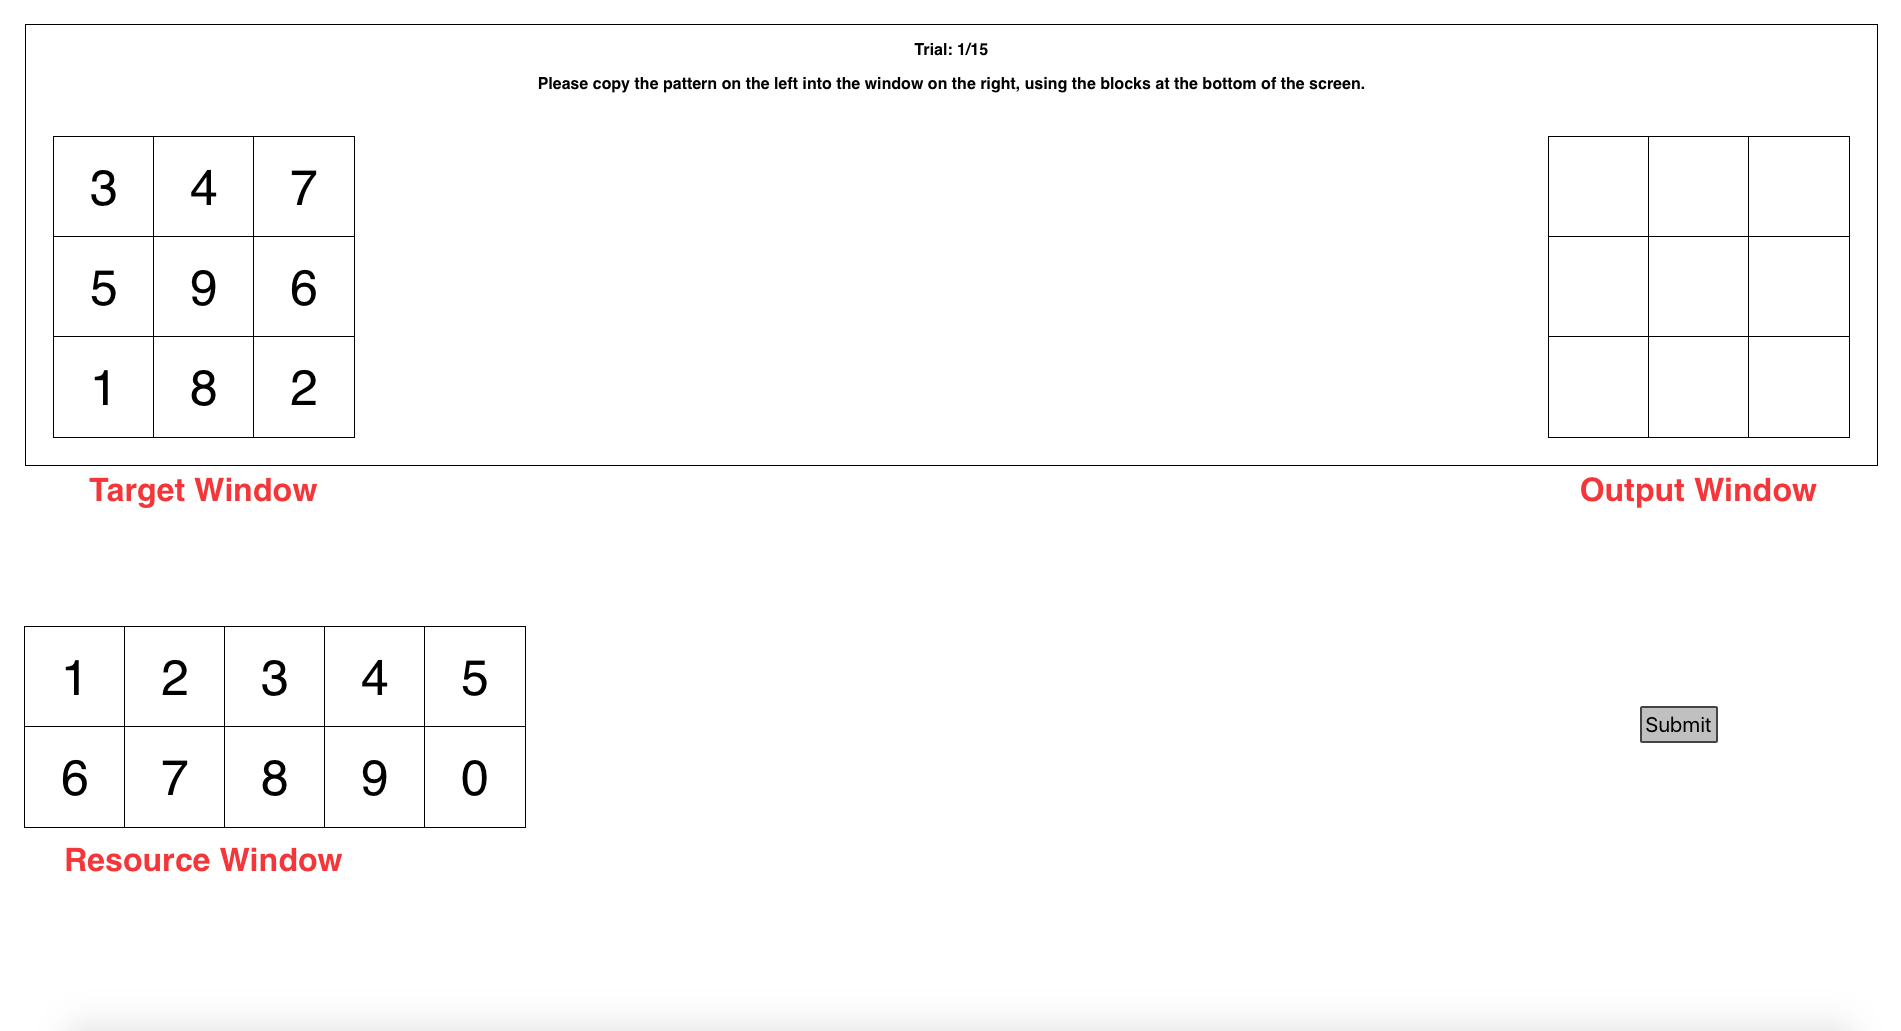
\includegraphics[scale=0.23]{images/ch34/ch4_numbers.png}}
\caption{The number condition.}
\label{fig:ch4_BWT}
\end{subfigure}
%\hfill%
\begin{subfigure}[b]{0.5\textwidth}
\centerline{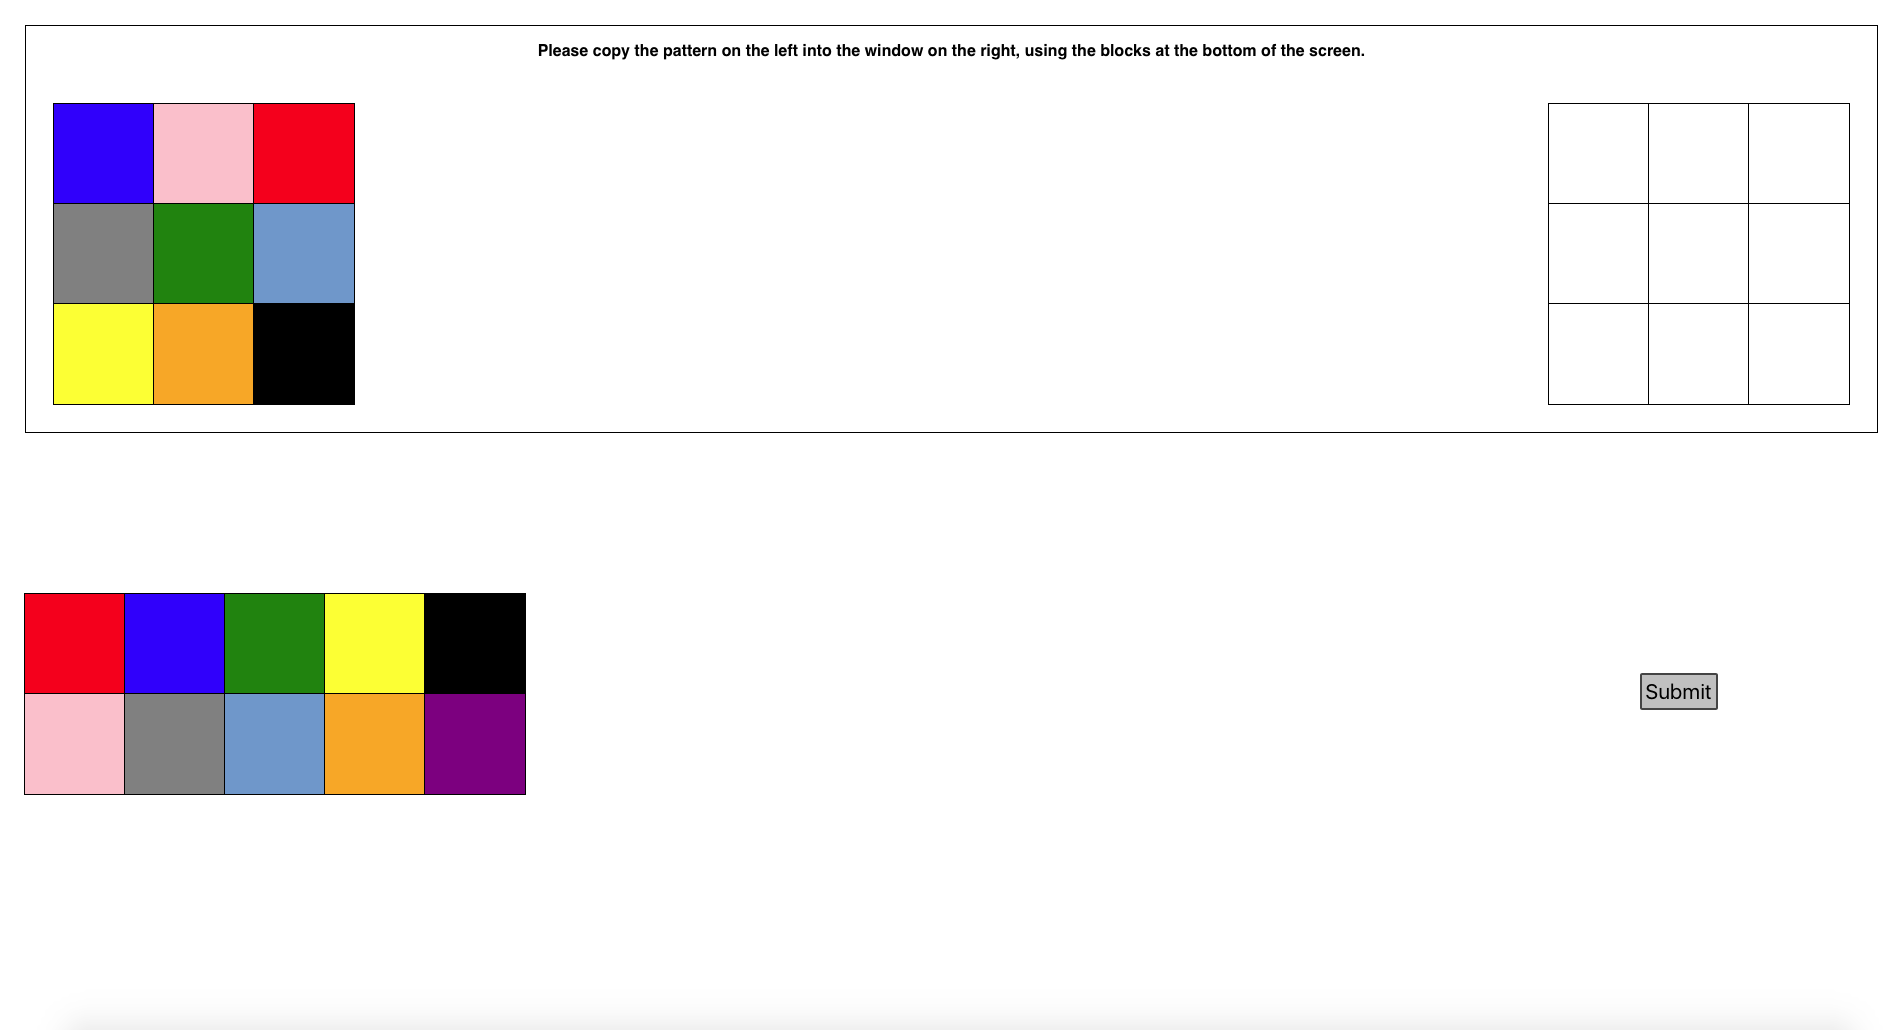
\includegraphics[scale=0.23]{images/ch34/ch4_colours.png}}
\caption{The colour condition.}
\label{fig:ch4_NWT}
\end{subfigure}
\caption[Study 3 task lay-out]{The task lay-out with the three different components.}
\label{fig:ch4_taskparadigm}
\end{center}
\end{figure}

\subsubsection{Design}
A mixed design was used with two independent variables: time cost and block type. The between-participants variable was the level of time cost which had three levels. If the Cost was Low, the target pattern was permanently visible. In the Medium and High Cost conditions, the target pattern was covered with a grey mask, and could only be uncovered by moving the mouse cursor over the window. The mask reappeared as soon as the cursor left the window. In the High Cost condition, there was an additional 1-second delay to uncover the mask. This delay time was used in previous BWT studies where it showed to have a significant effect on task strategies and performance \citep{Gray2006, Morgan2009, Waldron2007}. The within-participants variable was the block type to be copied, which was either coloured or numbered blocks. The order was counter-balanced across participants.

The dependent variables are listed in Table \ref{table:ch4_dvs}. For the Low Cost condition, the number and duration of visits to the target window were measured using eye fixations; consecutive eye movements within the target area were counted as one visit. Eye-tracking data was also obtained for the Medium and High Cost conditions. However, this eye-tracking data was not used for these conditions, as people were able to look at the target window area without uncovering and perceiving the target pattern. Therefore, in accordance with previous studies \citep{Morgan2009, Patrick2014, Waldron2007, Waldron2011}, for the Medium and High Cost conditions the frequency with which the target pattern was uncovered was used as a measurement for visits to the target window. These uncoverings were measured by Javascript. Both the usefulness and limitations of using these measures are discussed in the Discussion.
 
The number of blocks copied after each visit were measured by Javascript, which recorded all drop events of blocks into the output window. The position where it was placed on the 3x3 grid was used to determine whether the block was placed correctly.
The primary focus is on the measures of the first visit, as participants do not have any information yet on the target pattern. On subsequent visits, they may already have partial information in their head from previous visits. Therefore, the items copied after the first visit is believed to be the most 'sensitive measure of performance' \citep{Janssen2012}. 

Two measures were used to assess accuracy. Incorrectly placed blocks measured instances where a participant initially placed a block in the incorrect place, but then moved this to the correct place prior to submitting the pattern. Incorrectly submitted trials measured instances where the participant had finished copying a pattern and clicked the Submit button, but the pattern was incorrect.

\begin{table}[htp]
\centering
 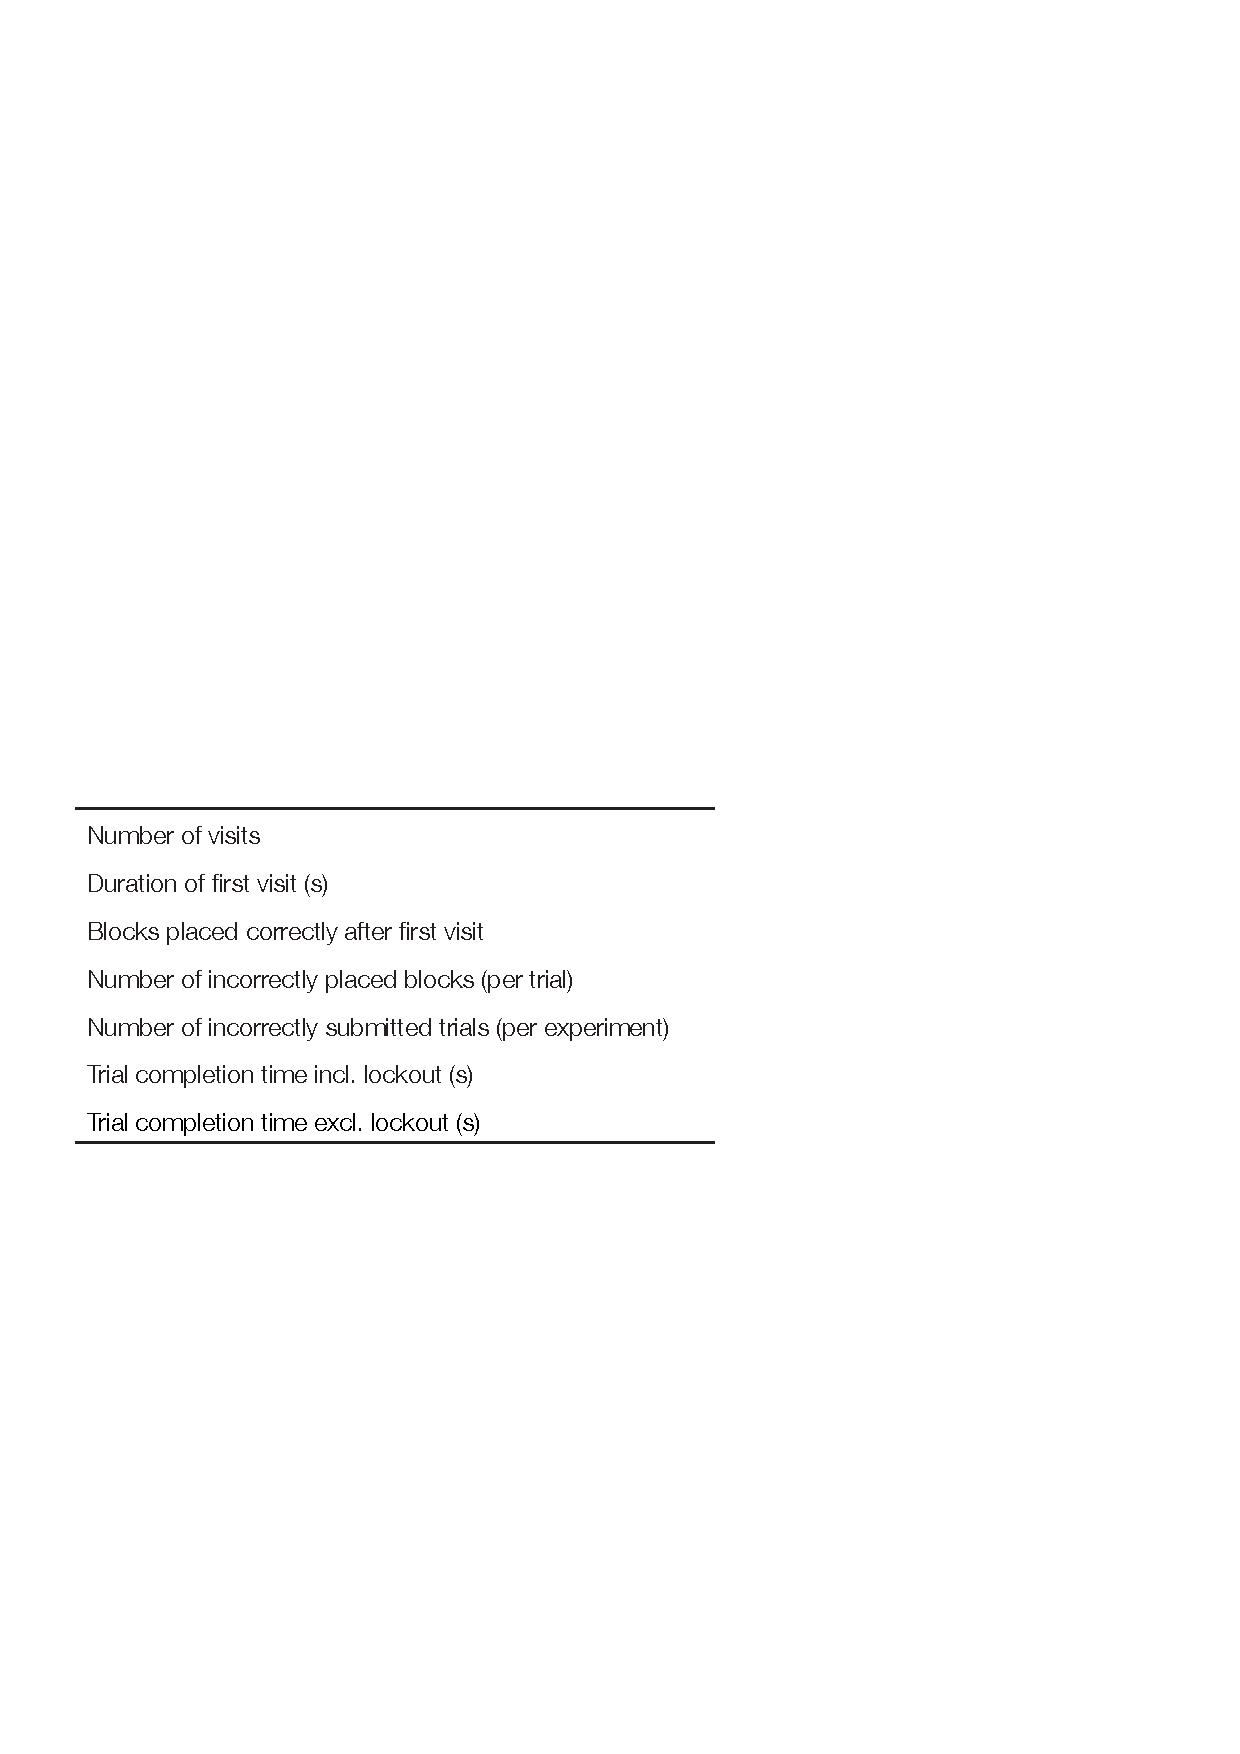
\includegraphics[width=0.6\textwidth]{images/ch34/ch34-3_DVs.pdf}
    \caption[Study 3 dependent variables]{Dependent variables used in the study.}
    \label{table:ch4_dvs}
\end{table}

\subsubsection{Procedure}
Participants were welcomed and briefed about the experiment. It was explained they would be shown nine blocks which were in a certain order, and had to copy this order by moving blocks around. Participants were instructed to complete the task as fast as possible, but it was explained that they were not able to continue until they had copied a pattern correctly. 

After the briefing, participants were asked to read and sign a consent form and were given an information sheet with a summary of the study and the researcher's contact details. In addition to the verbal briefing, the explanation of the study was written out on the computer screen for the participant to read and they were shown an instruction video that showed how the experiment worked. 
The experiment was broken down in two parts, one where they had to copy colours, and one where they had to copy numbers. For each part, they were given two practice trials first to get familiar with the set-up, and to give them a chance to ask questions if anything was unclear. There was an opportunity for the participant to take a break between the two parts. The study took around 20-30 minutes to complete.

\begin{comment}
\subsubsection{Ethical considerations}\label{sec:quanethics}
The study was undertaken with ethical approval from the UCL Research Ethics Committee [Project ID Number UCLIC/1415/001/Staff Brumby/Borghouts]. 
At the start of each study, participants were first briefed verbally about the study. They were asked to read and sign a consent form, and were given an information sheet to keep. This information sheet contained a summary of the study information and the researchers' contact details. It was explained that an eyetracker would record their eye fixations and movements, but that these recordings were anonymous and that they would not be directly identifiable. After participants had completed the first part of the experiment, a prompt appeared on the screen advising them to take a short break. Participants could take a break as long as they wanted and could decide themselves when to continue with the second part of the experiment.

Participants were informed that the data would be used for research purposes only and stored in accordance with the Data Protection Act 1998. They were also informed that their data would be anonymised and when used in a report or academic paper, their data would not be directly identifiable.
\end{comment}

\subsection{Results}
The means and standard deviations of all dependent variables are shown in Table \ref{table:ch4_IACmeans}. Two-way mixed ANOVAs were used to analyse the effect of time cost and block type on the dependent variables. A p-value of 0.05 was used for assessing the significance of all statistical tests. 

\subsubsection{Cleaning the data}
Eight participants were removed from the analysis due to weak eye-tracking calibration. Furthermore, one participant misunderstood the experiment and did not know she was allowed to uncover the mask of the target window more than once. This participant had scores that were more than three times the interquartile range from the rest of the participants' scores on six different variables, so this participant was considered an outlier and removed from the analysis. 

\begin{table}
\centering
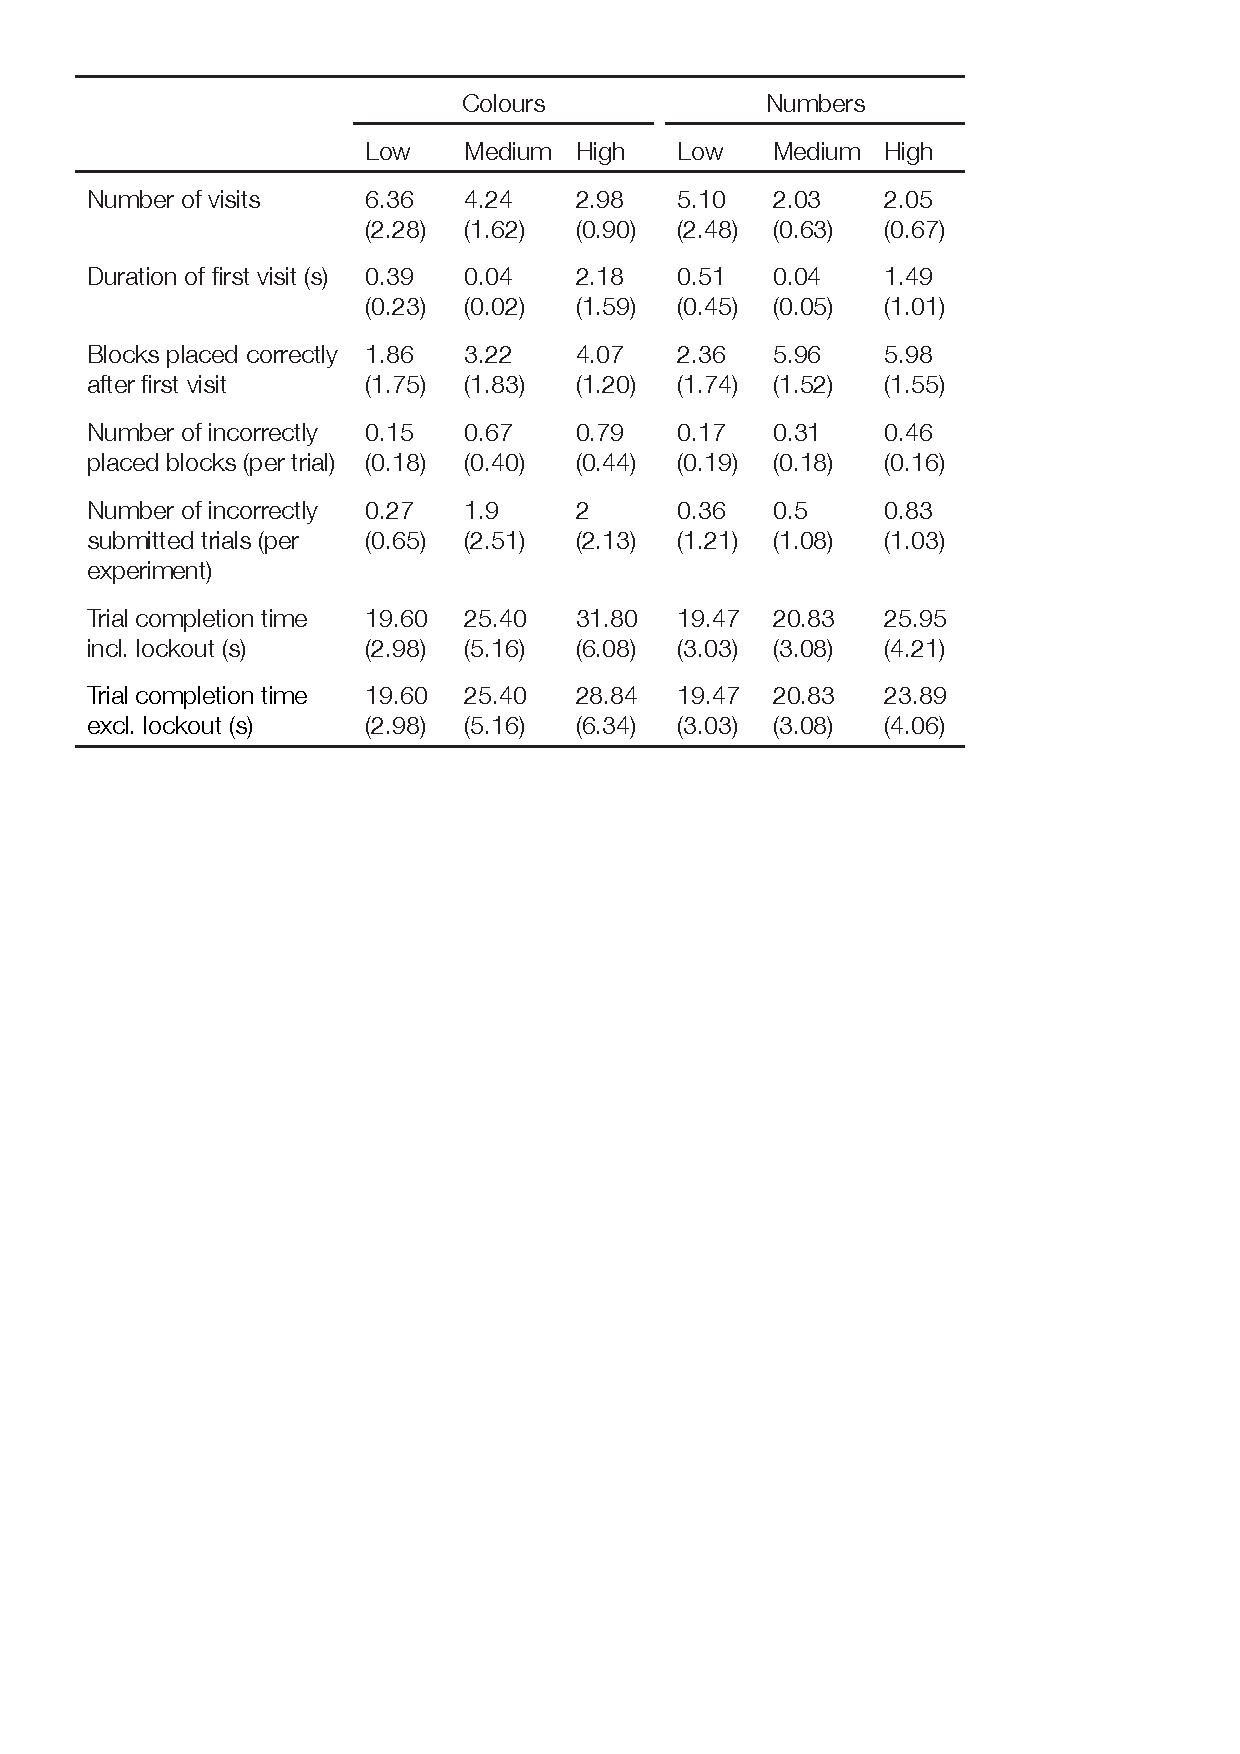
\includegraphics[width=0.8\textwidth]{images/ch34/ch34-3_Means.pdf}
\caption[Study 3 descriptive measures]{The means (and standard deviations) of dependent measures for the different conditions.}
\label{table:ch4_IACmeans}
\end{table}

\subsubsection{Number of visits to the target window}
The number of visits was measured using eye fixations for the Low Cost condition, and the uncovering of the target pattern for the Medium and High Cost conditions. Participants made fewer visits to the target source when they had to copy numbers (M = 3.06, SD = 2.08) than when they had to copy colours (M = 4.49, SD = 2.18), F(1,30) = 41.62, p<.001, $\eta^2$  = .58. Participants also made fewer visits as IAC increased from Low (M = 5.73, SD = 2.41), to Medium (M = 3.13, SD = 1.65), to High (M = 2.51, SD = 0.91), F(2,30) = 15.16, p<.001, $\eta^2$  = .50. To investigate differences between conditions, post-hoc Tukey comparisons were performed. Results showed that participants made significantly fewer visits in the Medium-IAC condition than in the Low-IAC condition, p <.01. However, there was no difference in number of visits between the Medium-IAC and the High-IAC conditions, p=.59. Participants looked at the target window for colours more on every level of IAC, and so there was no significant interaction, F(2,30) = 2.82, p=.08, $\eta^2$  = .16. 

\begin{comment}
\begin{figure}[!ht]
\centering
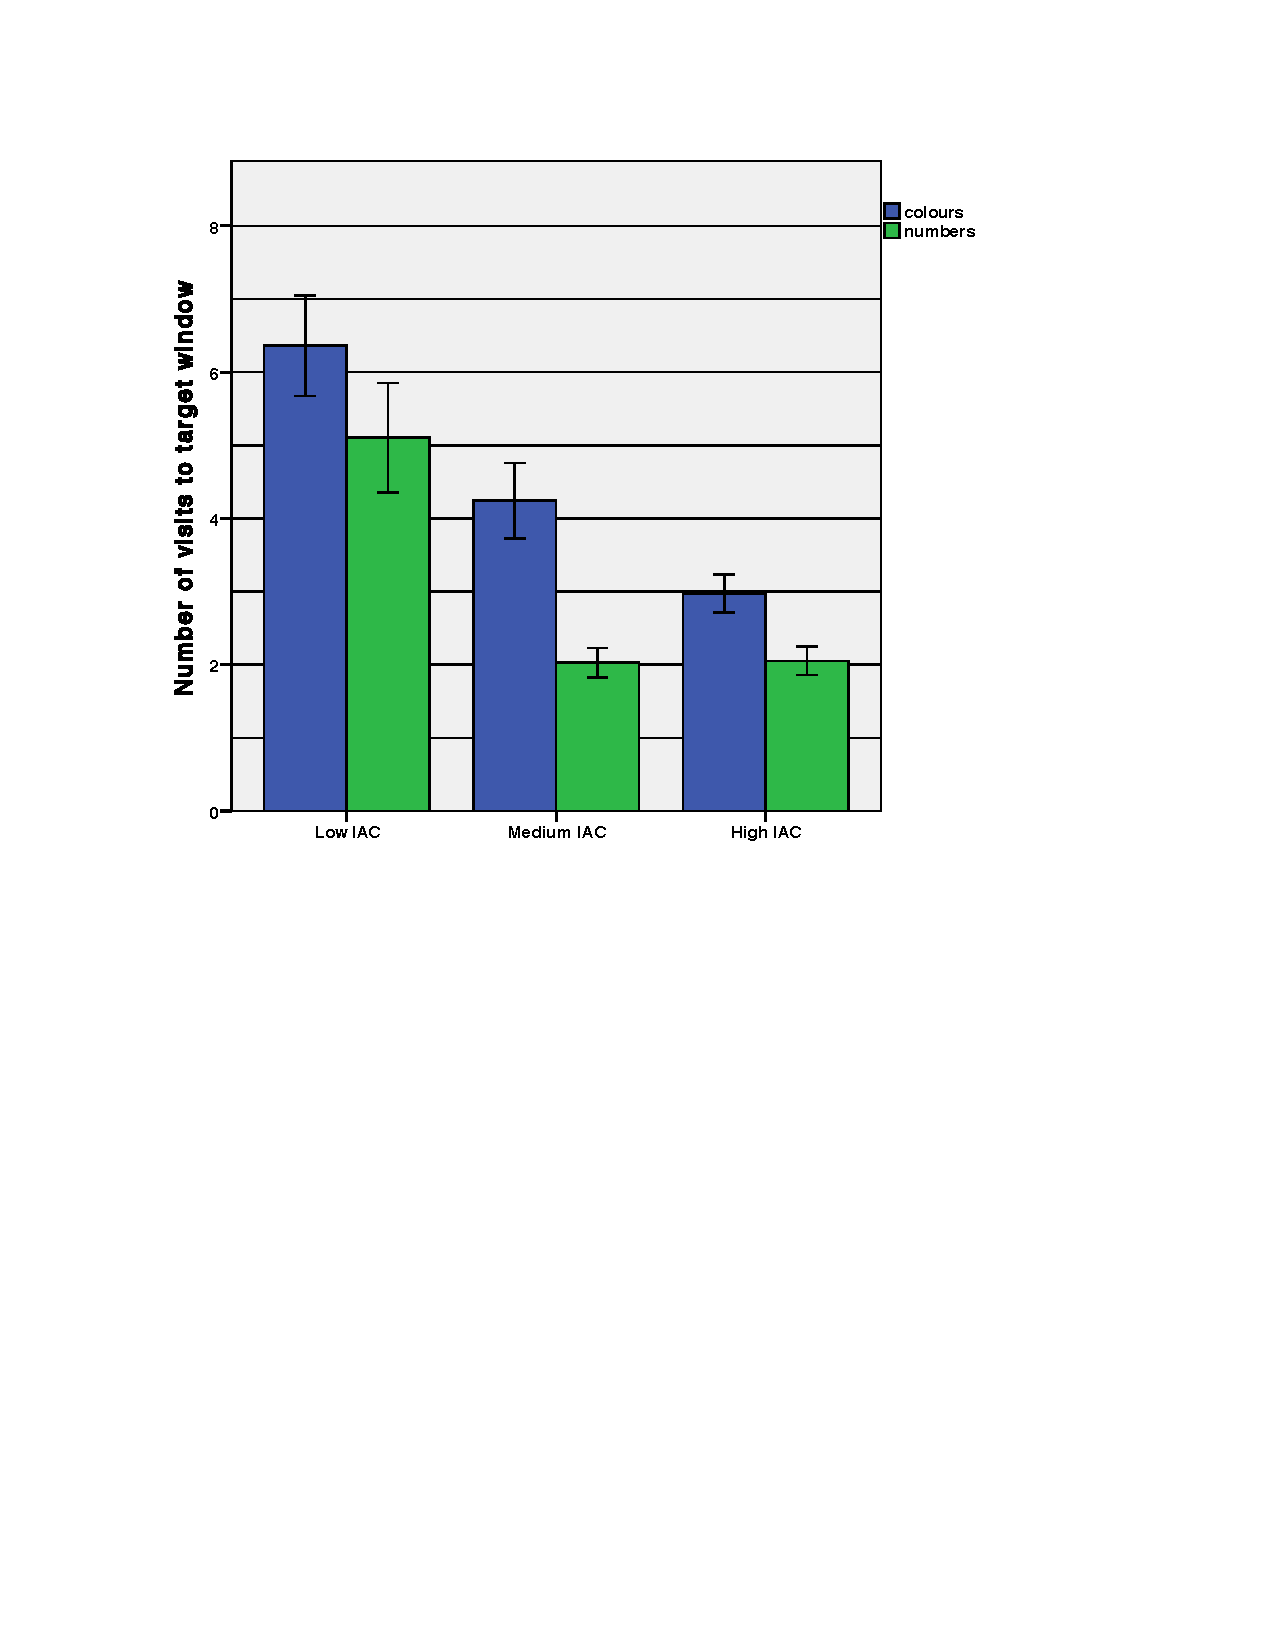
\includegraphics[width=\textwidth]{images/ch34/ch4_noVisits-bargraph.pdf}
\caption[Study 3 number of visits]{The interaction between block type and IAC for number of visits to the target window. The error bars represent $\pm $1 standard error.}
\vspace{-9pt}
\label{fig:ch4_noVisits}
\end{figure}
\end{comment}

\subsubsection{Duration of first visit to target window}
There was no significant main effect of block type on the duration of the first visit, F(1,30) = 3.05, p=.09, $\eta^2$  = .09. There was a significant effect of IAC, F(2,30) = 16.64, p<.001, $\eta^2$  = .53. Participants looked longer at the target source as IAC increased from Low to High. Post-hoc comparisons showed that participants looked longer in the High-IAC condition (M=1.84, SD = 1.35) than in the Low/Medium-IAC conditions, ps <.001. However, there was no difference in duration between the Low-IAC (M = 0.45, SD = 0.46) and the Medium-IAC (M = 0.05, SD = 0.04) conditions, p=.47. There was a significant interaction effect between IAC and block type, F(2,30) = 5.70, p<.01, $\eta^2$  = .28. There were no difference between block types in the Low-IAC condition, t(10) = -1.86, p = .09, nor the Medium-IAC condition, t(9) = -0.29, p = .70. However, in the High-IAC condition, participants looked significantly longer for colours (M = 2.18, SD = 1.59) than numbers (M = 1.49, SD = 1.01), t(11) = 2.76, p = .02.

\begin{comment}
\begin{figure}[!ht]
\centering
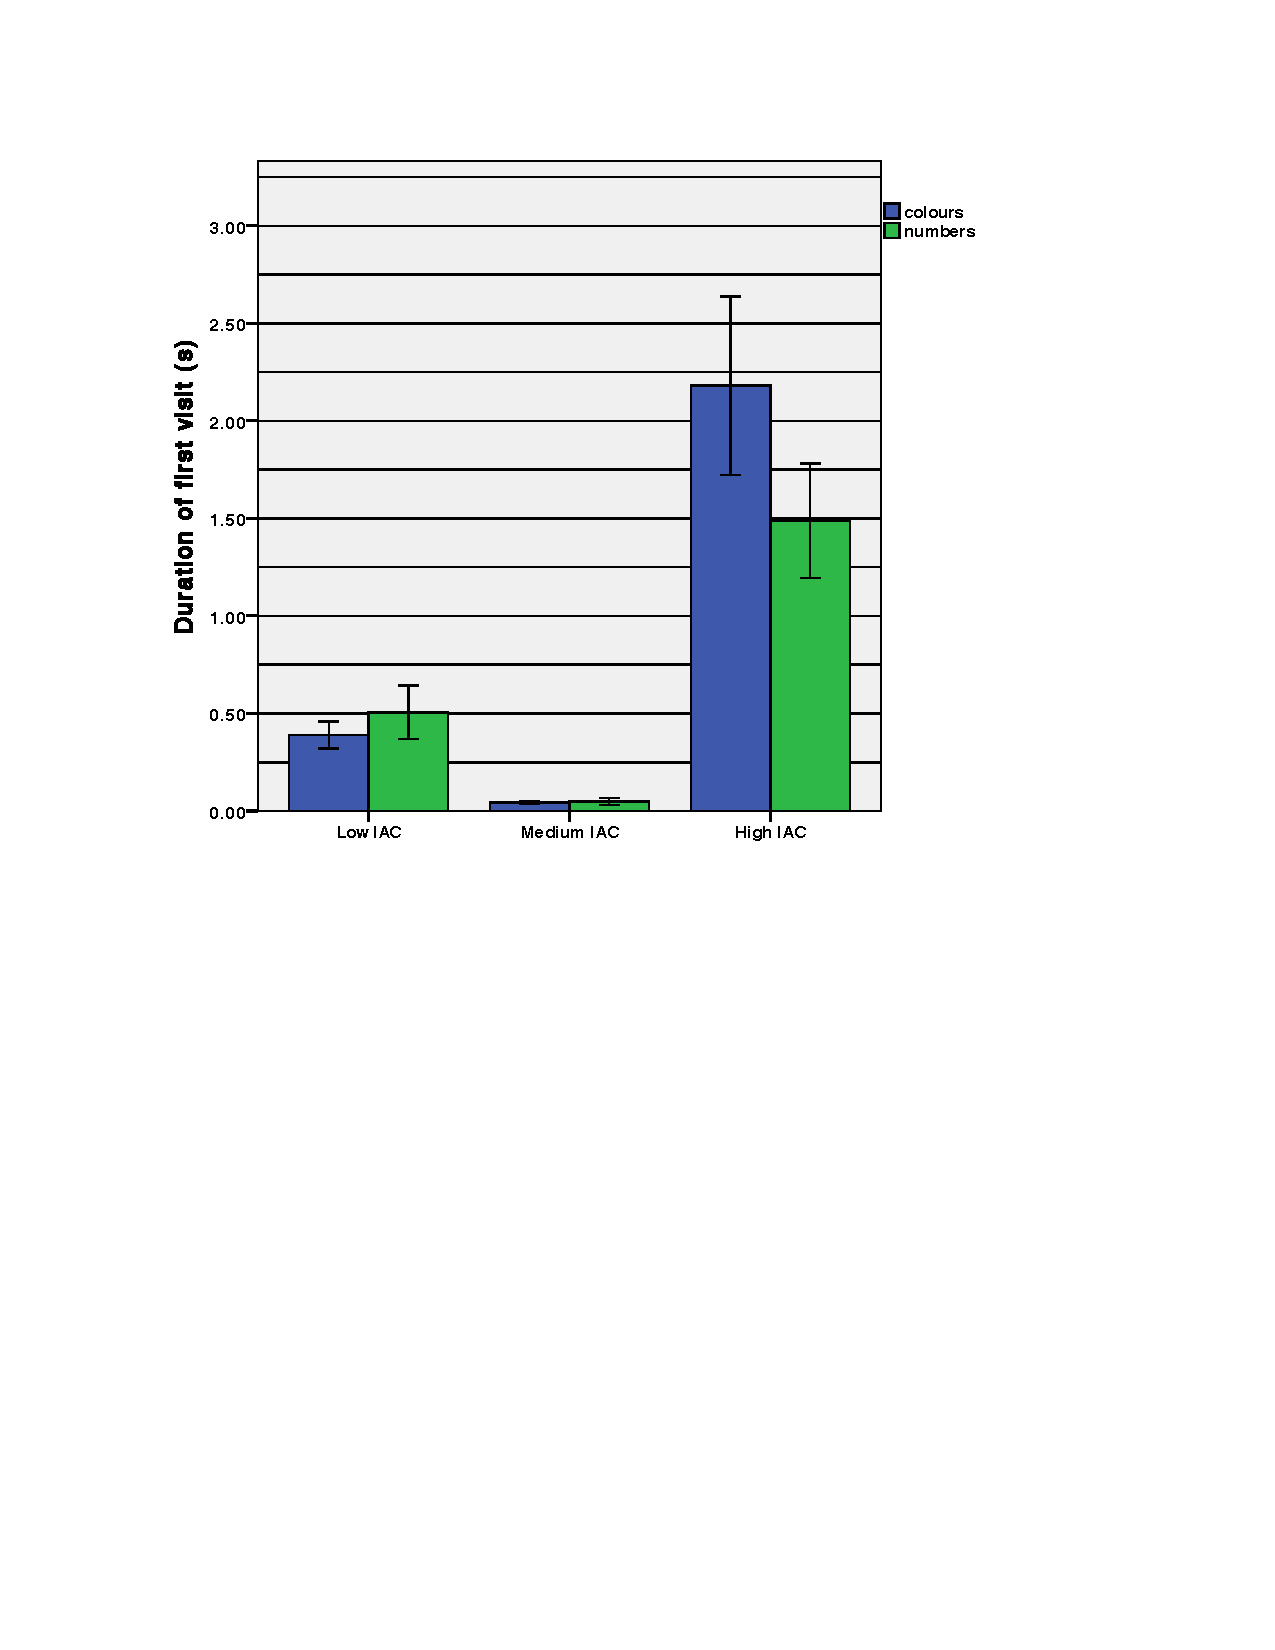
\includegraphics[width=\textwidth]{images/ch34/ch4_firstVisitDuration-bargraph.pdf}
\caption[Study 3 duration of first visit]{The effect of IAC on the duration of the first visit to the target window. The error bars represent $\pm $1 standard error.}
\vspace{-9pt}
\label{fig:ch4_firstVisitDuration}
\end{figure}
\end{comment}

\subsubsection{Blocks placed after first visit}
People placed more blocks correctly after the first visit for numbers (M = 4.77, SD = 2.33) than colours (M = 3.08, SD = 1.81), F(1,30) = 63.86, p<.001, $\eta^2$  = .68. They also placed more blocks as IAC increased, F(2,30) = 12.54, p<.001, $\eta^2$  = .46. Tukey post-hoc comparisons show there was a difference between the Low IAC and Medium/High IAC conditions (ps<.01), but not between Medium and High IAC conditions (p=.77). There was a significant interaction effect between IAC and block type, F(2,30) = 8.96, p<.01, $\eta^2$  = .37. When IAC was Low, the number of blocks that were copied correctly after the first visit did not differ significantly for colours or numbers.

\begin{comment}
\begin{figure}[!ht]
\centering
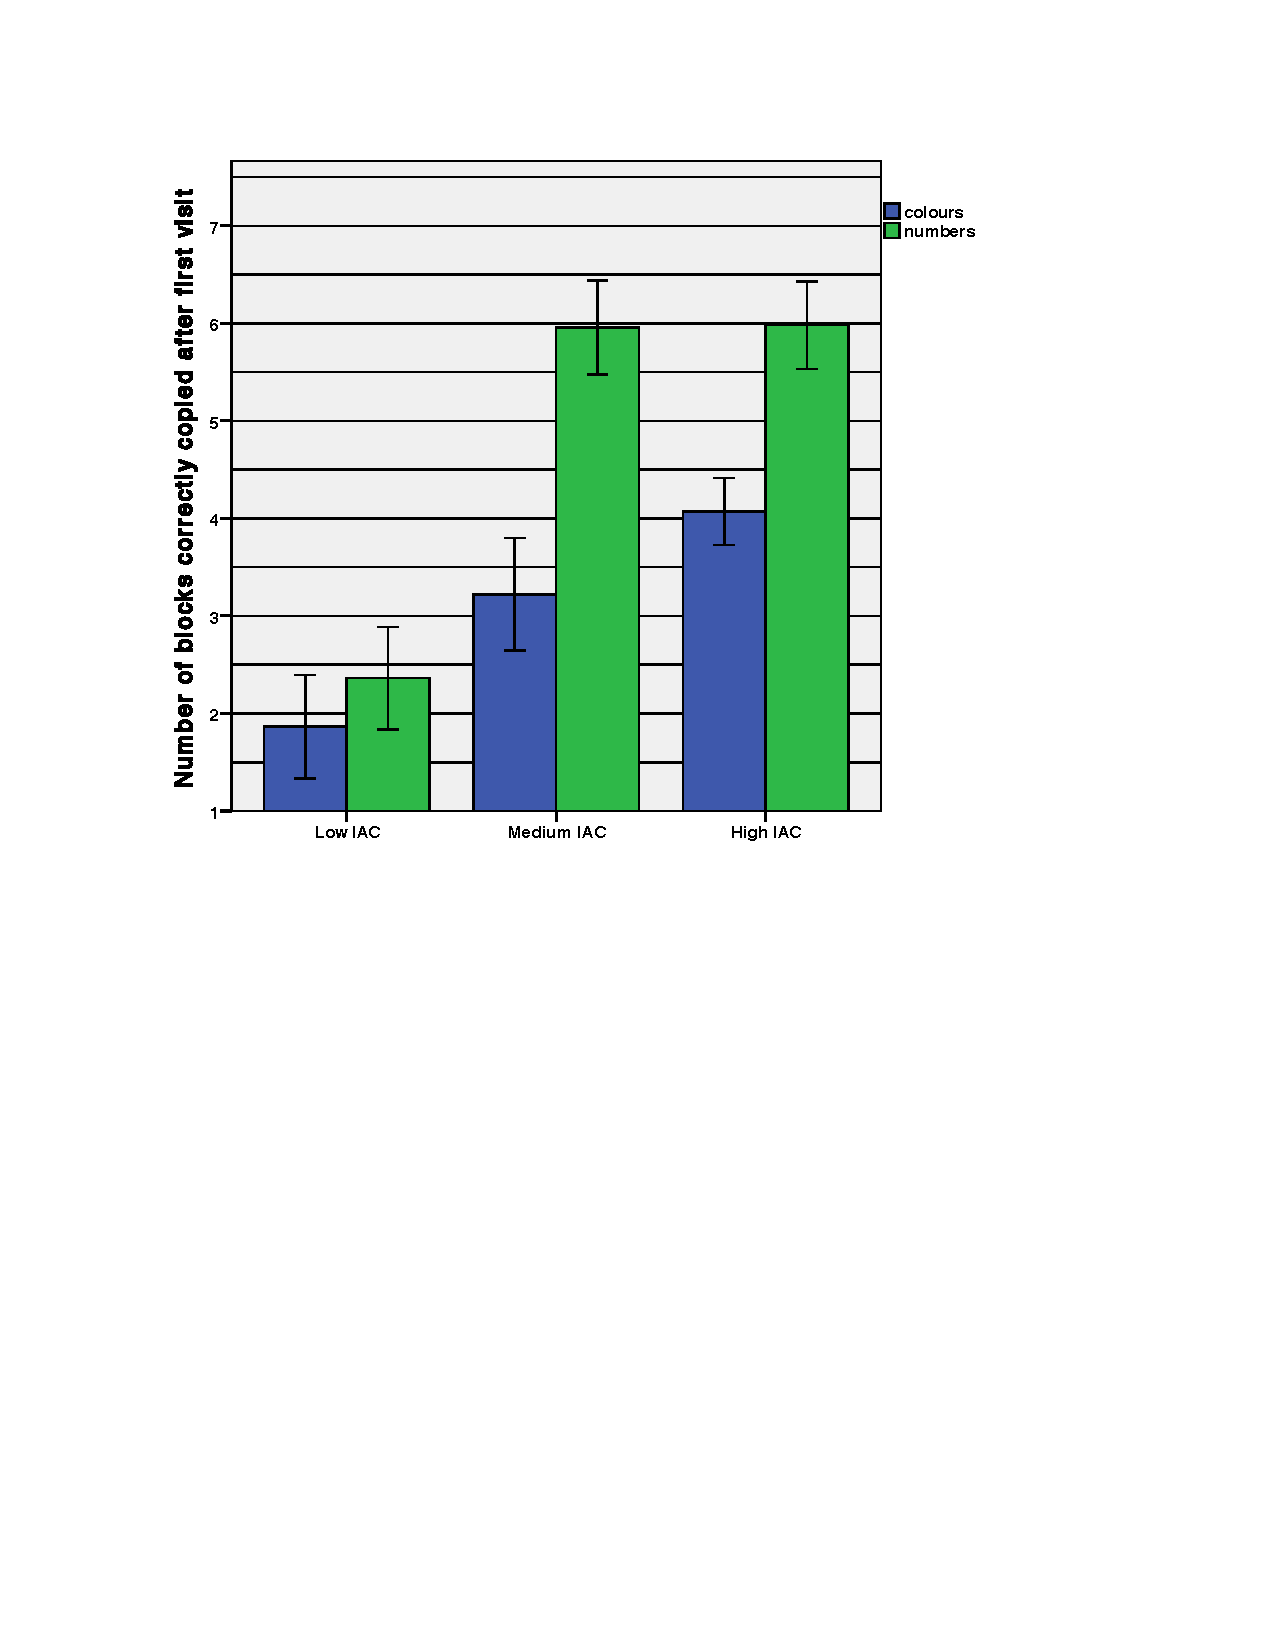
\includegraphics[width=\textwidth]{images/ch34/ch4_firstCorrectBlocks-bargraph.pdf}
\caption[Study 3 number of blocks correctly placed]{The interaction between block type and IAC for number of blocks correctly placed after the first visit to the target window. The error bars represent $\pm $1 standard error.}
\vspace{-9pt}
\label{fig:ch4_firstCorrectBlocks}
\end{figure}
\end{comment}

\subsubsection{Trial completion time}
Two trial completion times are considered here: total time and time excluding lockout. 
Looking at the actual completion time, participants took longer to complete a trial when they were copying colours (M = 25.80, SD = 7.06) compared to when copying numbers (M = 22.24, SD = 4.47), F(1,30) = 44.09, p<.001, $\eta^2$ = .60. As IAC increased from Low to Medium to High, participants took longer to complete a trial, IAC, F(2,30) = 15.91, p<.001, $\eta^2$ = .52. Tukey post-hoc comparisons show there was a difference between Low/Medium and High (ps<.01), but not between Low and Medium (p = .12). There was a significant interaction effect between IAC and block type, F(2,30) = 11.05, p<.001, $\eta^2$ = .42. When IAC was Low, completion time did not differ significantly for colours or numbers, but as IAC increased, participants were slower to copy colours.

With the lockout time in the High-IAC condition removed, the same effects were found for block type, F(1,30) = 34.55, p<.001, $\eta^2$ = 0.54, and IAC, F(2,30) = 8.18, p<.01, $\eta^2$ = .35. Tukey post-hoc comparisons show there was still a difference between Low and High (p<.01), but no longer between the Medium IAC and Low IAC or High IAC conditions (ps >.1). There was again a significant interaction effect between IAC and block type, F(2,30) = 8.13, p<.01, $\eta^2$ = .35.

\subsubsection{Number of incorrectly placed blocks}
Participants placed more blocks incorrectly for colours (M = 0.54, SD = 0.45) than numbers (M = 0.32, SD = 0.21), F(1,30) = 10.72, p<.01, $\eta^2$ = .26. %p= 0.003
As IAC increased and participants were keeping more items in memory, they increasingly placed more incorrect blocks, F(2,30) = 14.71, p<.001, $\eta^2$ = .50. Tukey post-hoc comparisons show there was a difference between the Low IAC condition (M = 0.16, SD = 0.18) and Medium/High IAC conditions (ps<.01), but not between the Medium (M = 0.49, SD = 0.35) and High IAC conditions (M = 0.63, SD = 0.36) (p = .30). There was a significant interaction effect between IAC and block type, F(2,30) = 3.36, p<.05, $\eta^2$ = .18. When IAC was Low, the number of blocks that were copied incorrectly did not differ significantly for colours or numbers, but as IAC increased, participants placed more blocks incorrectly for colours.

\subsubsection{Number of incorrectly submitted trials}
The number of trials that were submitted incorrectly was generally low, but participants submitted more incorrect trials for colours (M = 0.1, SD = 0.16) than numbers (M = 0.04, SD = 0.08), F(1,30) = 5.28, p=.03, $\eta^2$ = .15. There was no significant effect of IAC, F(2,30) = 2.70, p=.08, $\eta^2$ = .15, nor any interaction, F(2,30) = 1.65, p=.20, $\eta^2$ = .10.

\subsubsection{Qualitative data}
The screen recordings from the eye-tracker were played back to further investigate people's behaviour. Although this helped understand some behaviour which could not be determined from the quantitative data alone, these observations only serve to explain some of the quantitative measures and are not the main focus of the analysis.

The visit durations in the Medium IAC condition were suspiciously short. Upon replaying the screen recordings, it appeared that participants often accidentally moved their cursor over the grey mask of the target source. This was counted as a visit by the program, even though participants may have not intentionally moved their cursor to this part of the screen to look at the target source. They did not spend a long time looking at the target window, but also did not immediately move blocks either, and sometimes waited multiple seconds before they made a move. 

\begin{figure}[!ht]
\centering
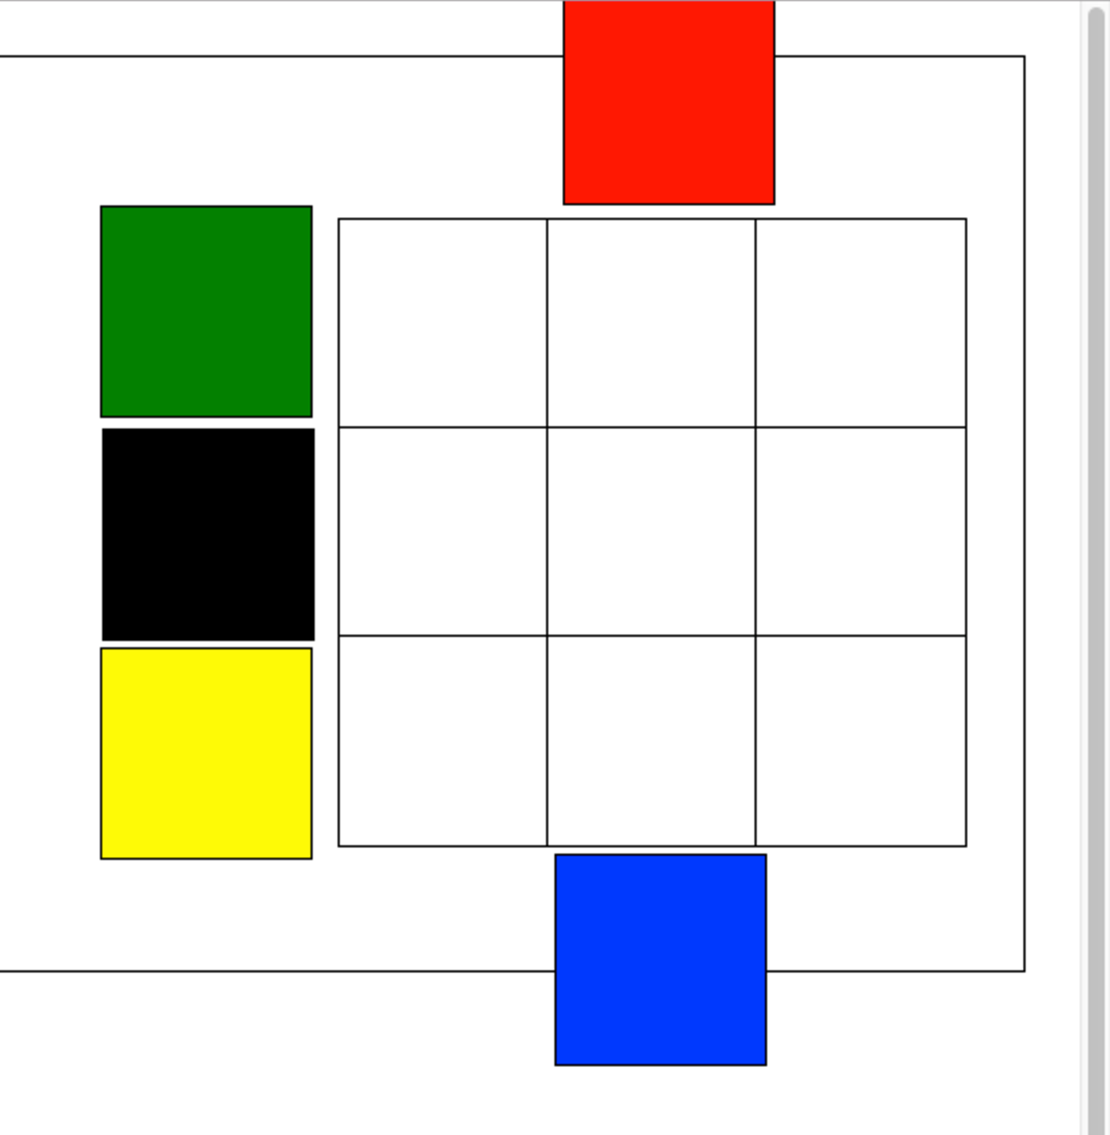
\includegraphics[scale=0.3]{images/ch34/ch4_placeholders.pdf}
\caption[Study 3 placeholders]{Participants placed blocks outside of the output window as `placeholders'.}
\vspace{-9pt}
\label{fig:ch4_placeholders}
\end{figure}

During the 1-s lockout in the High IAC condition, participants changed their minds about visiting the target window on numerous occasions. They placed their mouse cursor on the mask, but left this field before it was uncovered to move one or more blocks. It could be this decision also occurred in the Medium IAC condition, but as there was no lockout the mask was already uncovered before people made this decision, and would explain the very short visits.

People sometimes placed the blocks as 'placeholders' as shown in Figure \ref{fig:ch4_placeholders}: they placed several blocks outside of the output window next to the position they thought it belonged to, but did not place it there yet. Only after viewing the target again, they placed the blocks in the output window. Looking at quantitative data alone, this type of strategy would be depicted as one long view at the target, after which all blocks were placed in one go. This is true to some extent, but as people could already place the blocks and offload their memory without this being recorded by the program, they only had to check if this position was correct on the subsequent visit, and is different from a strategy where people spent a long time trying to memorise the blocks after which all blocks were placed.

\newpage

\subsection{Discussion}
The aim of this study was to investigate the effect of time costs on the number and duration of inquiries, and the effect on task performance. The main findings are:

\begin{itemize}
\item
increases in time costs make people adopt memory-intensive strategies
\item
the effect of a memory-intensive strategy on task performance depends on the type of information
\item
the effect of a memory-intensive strategy on task performance depends on the type of task
\end{itemize}

%The study replicated the BWT study to investigate whether the effect of time costs, as found in previous experimental studies, would extend to different types of information. We learn that people try to avoid time costs, and as time costs increase minimise switches to task information, and instead rely on information in their head. The study shows that the type of information matters: contrary to copying colours, when copying numbers this strategy did not increase any errors so may be a safe strategy, although it did not increase people’s performance either. 

%We also learn that the type of task matters: slowing people down, but not realistic. 

%Memory-intensive strategy
The effect of time costs on people's strategies is consistent with prior work \citep{Gray2006, Morgan2009, Waldron2007}. People switched from a perceptual to a memory-based strategy by making fewer but longer visits to the target window and placing more blocks immediately after the first visit. This further confirms that in a controlled setting, people are sensitive to small increases in time costs and try to avoid time costs.

In the Colours condition, a memory-intensive strategy worsened participants' task performance, as they took longer to complete the task and placed more incorrect blocks throughout the trials. In the Numbers condition, this strategy did not increase errors, which shows that the type of information matters when considering whether a memory-intensive strategy is beneficial or not. Numbers were likely easier to memorise, which was demonstrated by the higher number of blocks that were copied after a first visit to the target window: on average, people placed six numbered blocks after a first visit, which is about the number of items people can hold in short-term memory \citep{Miller1956}. In comparison, people only placed on average three coloured blocks after a first visit. Numbers can be rehearsed, and therefore refreshed in working memory, whereas visuo-spatial information such as coloured blocks is more difficult to memorise \citep{Baddeley1974}. 

Contrary to prior work however \citep{Gray2004, Soboczenski2013}, a memory-based strategy when copying numbers did not make people more efficient or accurate, which could have been due to the nature of the task. The error rate was overall low and upon reflection the interaction of moving blocks may have made people sufficiently slow to hardly make any errors. In previous studies, people typed in data using a computer keyboard, in which it is more likely to make data entry errors due to slips \citep{Oladimeji2011}.
 
 \subsubsection{Limitations}
The study used a similar manipulation of time costs as in previous BWT studies \citep{Morgan2009, Patrick2014, Waldron2007, Waldron2011}: in the Low Cost condition, the information was permanently visible, and in the Medium and High Cost conditions, the information was covered by a grey mask. Using this manipulation, it was difficult to measure visits to the target window in the same manner for all conditions. For the Low Cost conditions, eye fixations were used, whereas for the Medium and High Cost conditions, uncoverings of the mask were used. 

Measuring visits to the target pattern through eye fixations and mouse movements had a number of limitations.  
%Limitation of eye fixations: you do not know people are actually looking at the screen
First, while eye-tracking measures show how long and how often people are looking at a particular part of the screen, it can not reveal if people are actually perceiving or processing the data that is displayed \citep{Waldron2007}. Second, the results showed unexpectedly short visits for the Medium Cost condition. Playing back the screen recordings revealed that participants often accidentally uncovered the target window when they were moving their computer mouse, and it is therefore unclear if these uncoverings are a reliable measure of actual visits. Lastly, because visits were measured differently across conditions, the results from the Low-IAC condition may not be directly comparable with the Medium-IAC and High-IAC conditions. Therefore, for the next two experiments in this chapter the experimental setup was adapted so that participants had to make a conscious decision to reveal the target information, and were less likely to accidentally access the source when they did not intend to. Furthermore, the same consistent measure was used across conditions (i.e. a mouse click to make a window switch) to study inquiries. 

 %Limitation of uncoverings
% For the Medium and High Cost conditions, an interaction was required and a conscious decision had to be made to reveal the target in these conditions. It would therefore seem likely that uncoverings more reliably measure visits to the target window. However, the uncoverings for the Medium Cost conditions were rather short. Playing back the screen recordings suggests participants often accidentally uncovered the window, and it is therefore less clear if these are a reliable measure of actual visits. In future studies, the setup of the experiment should be designed so that participants make a conscious decision to reveal the target information, but do not accidentally access the source when they do not intend to. In the next two experiments, the same consistent measure is used (i.e. a mouse click to make a window switch) to study inquiries across conditions. 
 
 %Limitation of using different measuremenst 
% Second, visits were measured differently in different conditions, care should be taken to compare results from the Low-IAC condition with the Medium and High-IAC condition. 
 
 \subsection{Conclusion}
The aim of this study was to study the effect of time costs on number and duration of inquiries and task performance. The results show that if people retrieve all data from the same source, they will reduce switches between entering and looking up data if the access costs to this source increases. As it took more time to access, offloading behaviour was observed as well, and several participants prepared items they were going to need nearby, but did not use them yet. 

The overall aim of this chapter is to investigate the effect of time costs on inquiry strategies. Study 3 showed that time costs reduce number of switches and increases duration of switches. The task however only involved one source, in contrast with the task studied in Study 1 and 2, where people had to deal with various sources, all with different time costs. While we now have a better understanding of the effect of time costs on number and duration of inquiries, we do not know the effect on the timing of inquiries yet. This will be investigated in the next two studies.

%As a result, people not only have to make decisions on how often they make inquiries to these sources, but also when they interrupt their task to make inquiries.

\section{Study 4: Inquiries to multiple sources}\label{st:Study4}
 
\subsection{Introduction}
%Motivation
Study 3 showed people avoid time costs by making fewer inquiries to an information source. Participants tried to group and memorise as much information, in order to minimise the number of revisits to this source. In the experiment, all information was to be found on a single source. As discussed in Chapter \ref{ch:12}, data entry in office workplaces is often more complex than switching between a task and a single source: information can be spread over various sources with different time costs associated with them. Information can be one click away, or time has to be spent accessing it. What we do not know from Study \hyperref[st:Study3]{3} is how time costs affect how people schedule inquiries to different sources with different time costs. Observational findings from Study \hyperref[st:Study2]{2} suggest that inquiries with a high time cost are postponed: participants prepared physical information sources either before starting work or postponed it to access later. Digital information sources however were often accessed during the task, as these were presumed to be quick to retrieve. Furthermore, in prior work \citep{Sohn2008} information access cost was found to be a main factor that determined whether participants looked up information on their mobile phone as soon as they needed it, or whether they postponed to address it later. While these findings demonstrate people take time costs into account when accessing information on physical sources and mobile phones, it is unclear whether participants take time costs of switching windows on a desktop computer into account. Easy switching between windows on conventional desktop computers may give the false impression that information is easy to access \citep{Sellen2003}. 

The aim of Study \hyperref[st:Study4]{4} is to understand the effect of time costs on the timing of inquiries for a data entry task. An experiment was conducted in which participants had to complete a data entry task, and look up the to-be-entered items by switching to two different computer windows. While prior work has demonstrated that various tasks can involve the use of multiple information sources \citep{Cangiano2009, Murphy2016, Su2013}, it has not been measured how people access these sources, and to what extent the time cost to access a source influences these decisions. Based on the postpone strategies observed in Study \hyperref[st:Study2]{2}, the following hypothesis is made:

\begin{itemize}
\item [H1.]
As the experiment progresses and people become aware how costly it is to access certain sources, they will learn to postpone entering High-Cost items, and choose to enter the Low-Cost items first. 
\end{itemize}

Prior work has shown that increased time costs encourage people to learn more efficient strategies, which they then transfer to use in other situations in which time costs are no longer high \citep{OHara1998, Patrick2014, Waldron2007}. For instance, \citet{Patrick2014} conducted an experiment where participants had to complete a Blocks World Task. Some participants had permanent access to the target pattern, whereas other participants had to complete a number of trials first, in which the target pattern was hard to access. People who were exposed to the interface with an increased access cost first adopted a memory-based strategy and retained this strategy, even when they then interacted with an interface with lower access costs. It is therefore expected that once participants learn it is more efficient to group High-Cost items, they may adopt this strategy for Low-Cost items as well:

\begin{itemize}
\item [H2.]

As the experiment progresses, participants in the High-Cost conditions will learn and choose to enter all Low-Cost items in a batch, and then the High-Cost items in a batch, rather than looking up each item one by one.

\end{itemize}

\subsection{Method}
\subsubsection{Participants}
Thirty-three participants (21 female, 12 male) ranging from 18-52 years (M = 26, SD= 8) took part in the experiment. They were recruited from a university subject pool and received $\pounds$4 for their participation.

\subsubsection{Task}
The aim of the study was to study how people address inquiries from multiple sources for a data entry task. There are currently no existing tasks available that are suitable for this purpose: in existing task paradigms, all information is usually located on a single source. For the purpose of this experiment, I therefore created an experimental task. The experimental task was based on an expenses task, a routine data entry task observed in the studies in Chapter \ref{ch:12}. For this task, the user has to complete a number of data entries regarding incurred expenses in order to get the expenses reimbursed. They enter this into a claim form, which looks similar to a spreadsheet. 

For each trial, participants were presented with a data entry sheet consisting of two expense claims (see Figure \ref{fig:ch34_4-tasklayout}). They had to complete each row by entering a financial amount to specify an expense that was made, and an account code to specify which account to use to reimburse the expense. They retrieved these data items by switching to two other windows. One window contained the amounts (Step 1 in Figure \ref{fig:ch34_4-tasklayout}), and another window contained the account codes (Step 2 in Figure \ref{fig:ch34_4-tasklayout}). The participant could go to a window by clicking on the corresponding name in the horizontal menu at the top of the screen. Only one window could be viewed at a time and covered the full screen. 

\begin{figure}
 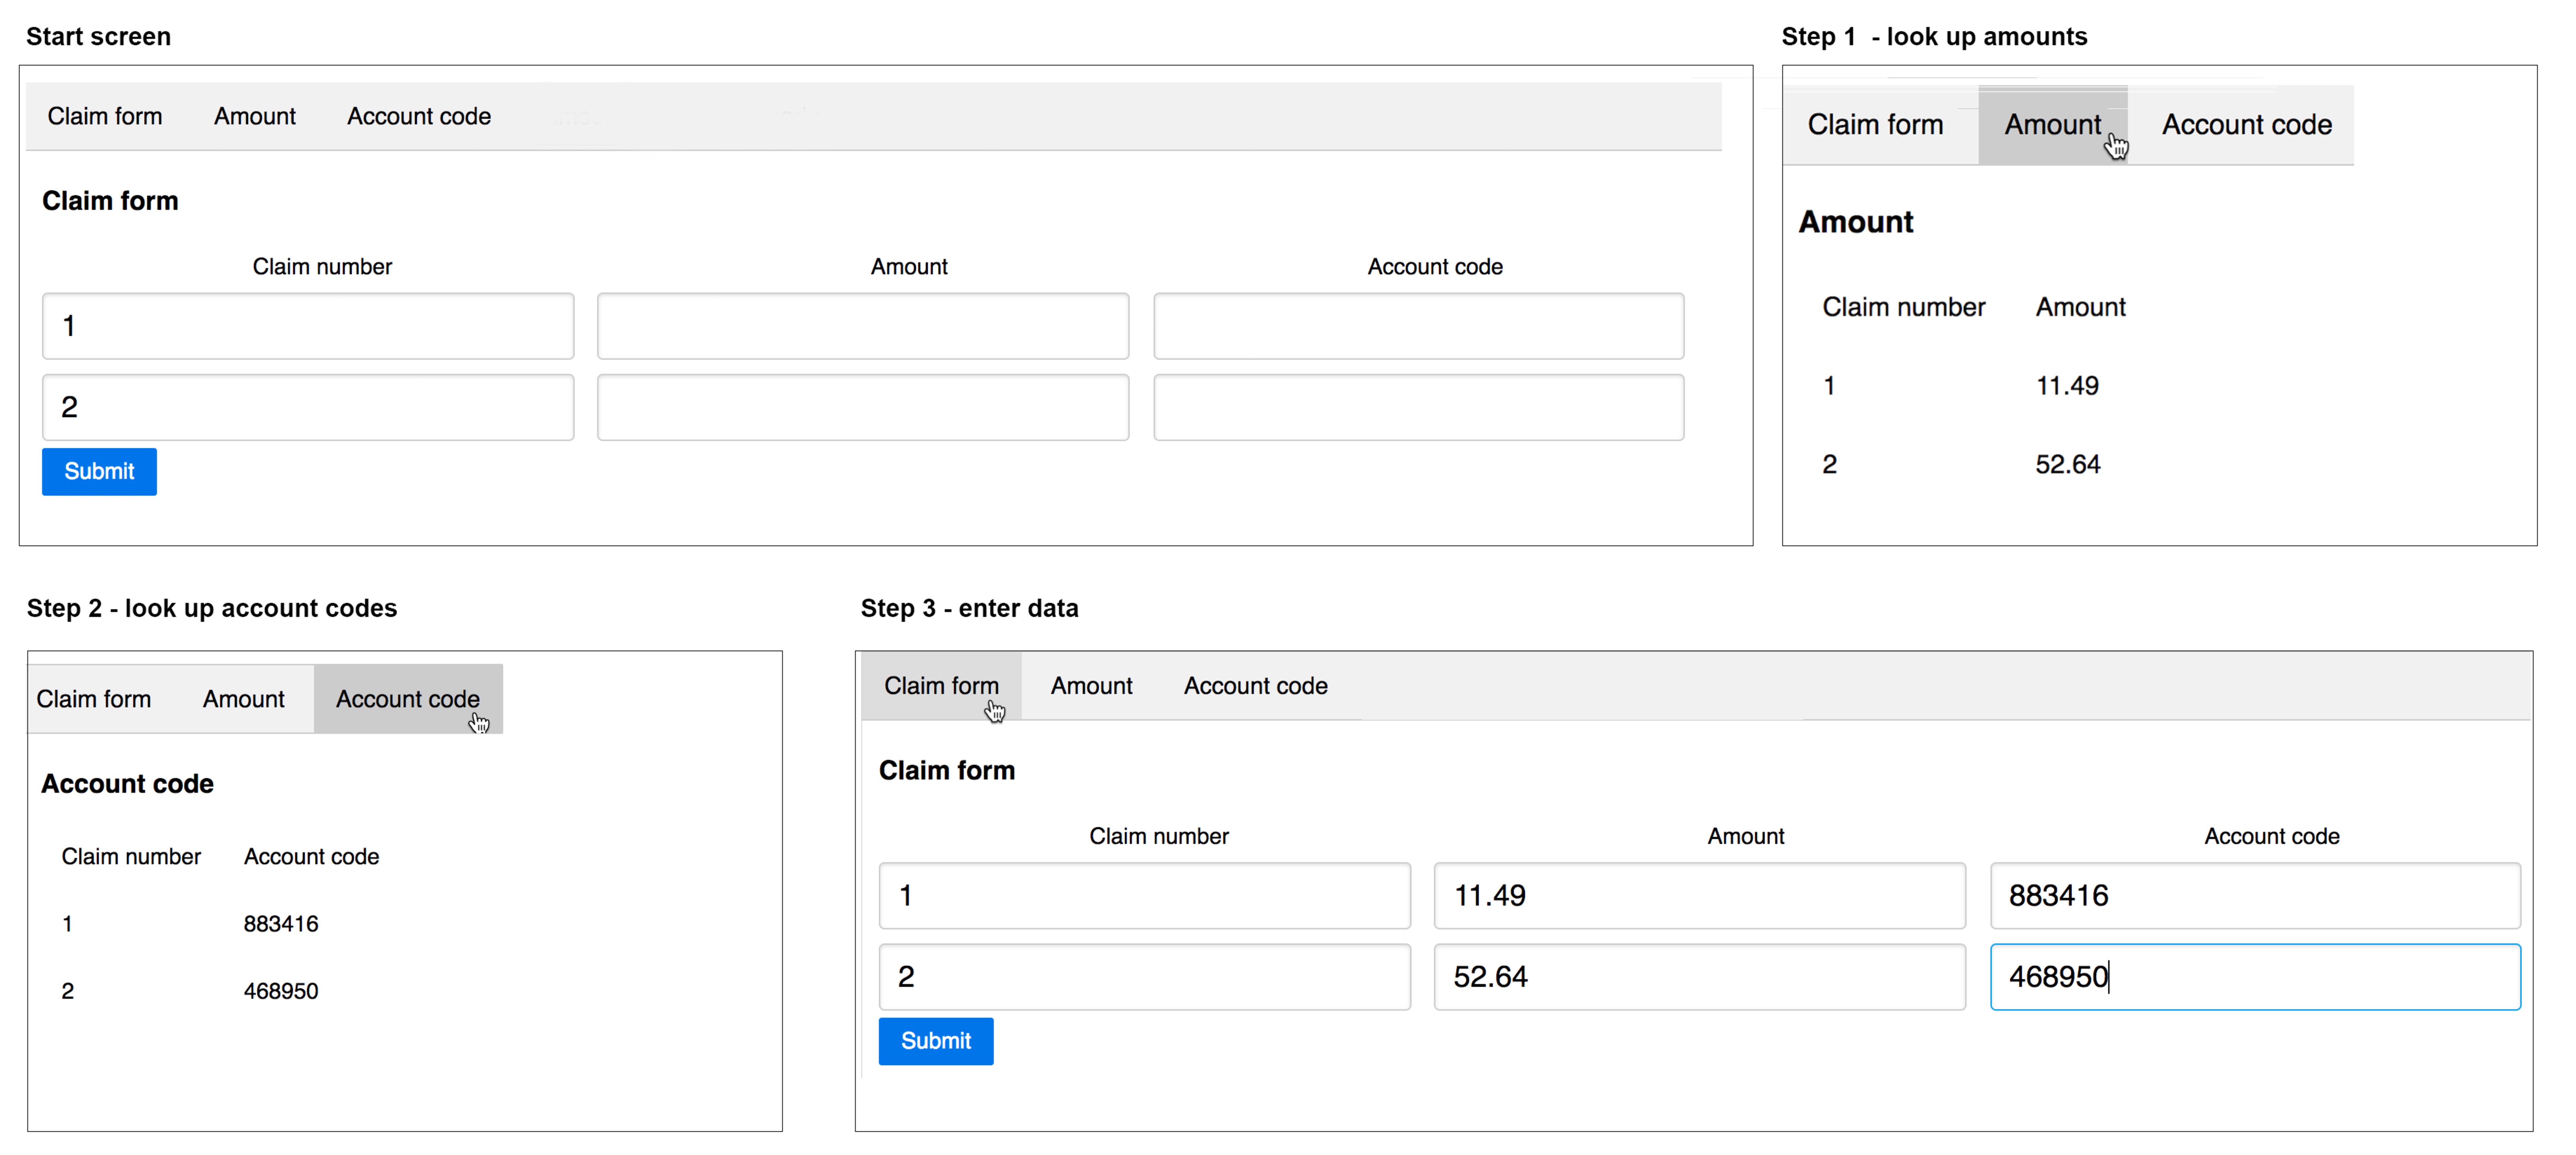
\includegraphics[width=\textwidth]{images/ch34/ch34-4_Tasksequence.pdf}
    \caption[Study 4 data entry task layout]{The data entry task. At the start of each trial, participants were presented with a data entry form with two expense claims, and had to enter four data items in a data entry form. The participant had to switch to an Amounts window (Step 1), and switch back and enter the correct amount in the correct place on the form (Step 2). The participant then had to switch to the Account code window (Step 3) , and switch back and enter the correct amount in the correct place on the form (Step 4). Step 1-4 were repeated for the other items, until all four items had been entered. The participant could switch back and forth between windows as often as needed.}\label{fig:ch34_4-tasklayout}
\end{figure}

\subsubsection{Materials}
The numbers to be entered were made to resemble values that are ecologically relevant to an expenses task. The account codes were similar to codes that are currently used by the universities studied in Chapter \ref{ch:12}, and have a fixed length of six digits (e.g. 654273). The string of digits was random with no particular pattern. Amounts consisted of two digits on the integer part and two digits on the fraction part (e.g. 11.95). 

The experiment was conducted in a maximised web browser on a desktop computer with a 24-inch monitor and a resolution of 2048x1152 pixels. Participants used a computer mouse and number keypad, and it was not possible to copy and paste information. If the participant switched from the data entry form to another window and back, the cursor stayed in the same data entry field. The task interface was developed in HTML, CSS, JavaScript and PHP. All mouse clicks, key presses and timestamps were recorded using JavaScript.

\subsubsection{Design}
A between-participants design was used with one independent variable, the presence or absence of a time cost when switching to one of the information windows. The time cost manipulation in the current study differs from Study \ref{st:Study3}, as the main focus here is to see how people manage inquiries that each have a \textit{different} time cost, as opposed to inquiries that all have the \textit{same} time cost. The manipulation is explained in more detail below. 

In the \textit{Low-Amount, Low-Account} (Low) condition, there were no delays in opening any of the windows. In the \textit{High-Amount, Low-Account} (High-AM) condition, there was a 2-s delay when opening the Amount window, and no delay when opening the Account window. In the \textit{Low-Amount, High-Account} (High-AC) condition, there was no delay when opening the Amount window, and a 2-s delay when opening the Account window. There were no delays in opening the data entry form in any of the conditions.

The Low condition was added as a control condition to understand strategies in a situation where all inquiries had the same time costs, and compare whether these differed from strategies in a High-Cost condition. A High-Cost condition only had a delay on one of the two windows, so that people were presented with both a low and high time cost. This manipulation enabled me to test the hypothesis that people postpone entering High-Cost items in a situation when they can enter Low-Cost items first. Furthermore, there were two high cost conditions, because there were two types of data to be entered (an amount and account code). To know whether any measured differences in inquiry strategies were due to time costs associated with opening a window, rather than the type of data item or the order in which the items were presented, there was one high cost condition where there was a high time cost to access amounts (and a low time cost to access account codes), and another high cost condition where there was a high time cost to access account codes (and a low time cost to access amounts). To simplify notation, from this point onwards these two different High-Cost conditions will be referred to as the High-AM condition and High-AC condition, respectively. 

%An additional condition where all windows had a high time cost is not included in the study, because the interest was not so much on how people access inquiries with the same time cost (regardless of whether it is low or high)

%The main interest of the study was to see how people prioritised inquiries with different time costs. 

%A between-participants design was used with one independent variable, the presence or absence of a time cost when switching to one of the information windows. In the Control condition, there were no costs in switching between any of the windows. In the High-Amount condition, there was a 2-s delay when opening the Amount window, and in the High-Account condition there was a 2-s delay when opening the Account window. There were no delays in switching back to the data entry form in any of the conditions. 

To investigate the timing of inquiries, the order in which participants entered the data items was analysed. On a trial-by-trial basis, the main dependent variable was whether people interleaved between expenses or not: did participants enter the data items in sequential order (i.e. enter one expense first, and then the second expense), or did they interleave between the two expenses to enter items from the same source first (i.e. enter all amounts first, and then all account codes)? Two values had to be entered for each expense: an amount and an account code. If participants entered the amount and account code of one expense before entering the other expense, this was considered a sequential order. If participants entered amounts of each expense first, followed by entering the account codes or vice versa, this was considered interleaving. All window switches and key presses were recorded to determine in which order data was entered. Window switches were recorded to capture the number and duration of switches to information windows. Other dependent variables were trial completion time and data entry error rate. In addition, the type of errors was analysed. 

\subsubsection{Procedure}
The experiment took place in a closed quiet room. It was explained to participants that the task involved entering expenses, and that for each trial they had to enter two expenses. They were not instructed to use a particular strategy, but it was explained it was important to complete all data entry fields before proceeding to the next trial, as they could not return as soon as they had pressed 'Submit'. There were no restrictions in the number or duration of times they could switch between windows, or the order in which they completed the trial. One trial consisted of two expenses, i.e. four data entries. Participants first completed two practice trials to familiarise themselves with the task, and were free to ask any questions; data from these trials were not included in the analysis. After that, the experimental session consisted of 50 trials, divided into 5 blocks of 10 trials. After each block, there was an opportunity for the participant to take a short break. A prompt appeared on the computer screen, and the recording time was paused. Participants could carry on with the experiment by pressing a button on the screen. For each block, a set of 20 different amounts and 20 different account codes were used. These sets were re-used for every block, so in total, each number was presented five times throughout a session. The experiment took approximately 30 minutes.

\subsubsection{Pilot study}
Because the task was newly created for the study and had not been used in previous studies before, two pilot studies were conducted with colleagues to test the task as well as experimental design. The pilot studies were also intended to see if the length of the experiment was long enough for participants to learn and develop strategies, but not too long and tiring to complete.

During the pilot studies, there was a scheduled break after every 5 trials. Both participants mentioned the break prompts happened too frequently, and experienced them as disruptive. They did not find the experiment too long. One participant could not remember which computer windows had an increased time cost. As a result, he did not adapt his strategies according to anticipated time costs and kept entering the data items row by row. The second participant mentioned that the increased time costs definitely made her more careful in checking the numbers were correct. The participants were aware some of the numbers occurred more than once, but the numbers did not occur often enough to be able to memorise them. 

For the main experiments, the breaks were reduced to happen after every 10 trials. In addition, the names of information windows with an increased time cost were underlined in the horizontal menu. This visual feature was added to help users see more easily which windows had a delay.

\subsubsection{Data analysis of task strategies}
A bottom-up approach was taken to group and analyse people's data entry strategies. For the first iteration of analysis, each trial was grouped into one of two categories: a sequential or interleaving category. If participants first entered the amount and account code of one expense before entering the other expense, this trial was grouped in the sequential category. If participants entered amounts of each expense first, and then entered account codes, or the other way around, this trial was grouped in the interleaving category. On a small subset of trials (<1\%) neither of these strategies was chosen: for example, participants first entered the amount of one expense, followed by the account code of the second expense. These trials were also grouped in the interleaving category, as participants switched to entering the second expense before completing the first expense.

Mouse clicks to switch between windows were used to code the order of people's actions, and get insight into the order in which people visited and entered data items. During the second iteration of analysis, for each trial the order of actions was considered and the trial was either grouped under a new strategy group for this order, or the trial was grouped under an existing strategy group. The most common order of actions is shown in Figure \ref{fig:ch34_4-groupstr}.

\subsection{Results}
Table \ref{tbl:ch34_4-means} summarises the results of the dependent measures for the three conditions. The distribution of the interleaving rate, number and duration of visits, and the error rate were not normally distributed, so non-parametric Kruskal-Wallis tests were used to analyse effects of time costs on these dependent variables. 
A Shapiro-Wilk test suggested that the trial completion times did follow a normal distribution, \textit{W} = 0.95, \textit{p} = .10, so a one-way ANOVA was used to analyse the effect on trial times. A p-value of 0.05 was used for assessing the significance of all statistical tests. 

\begin{table}
 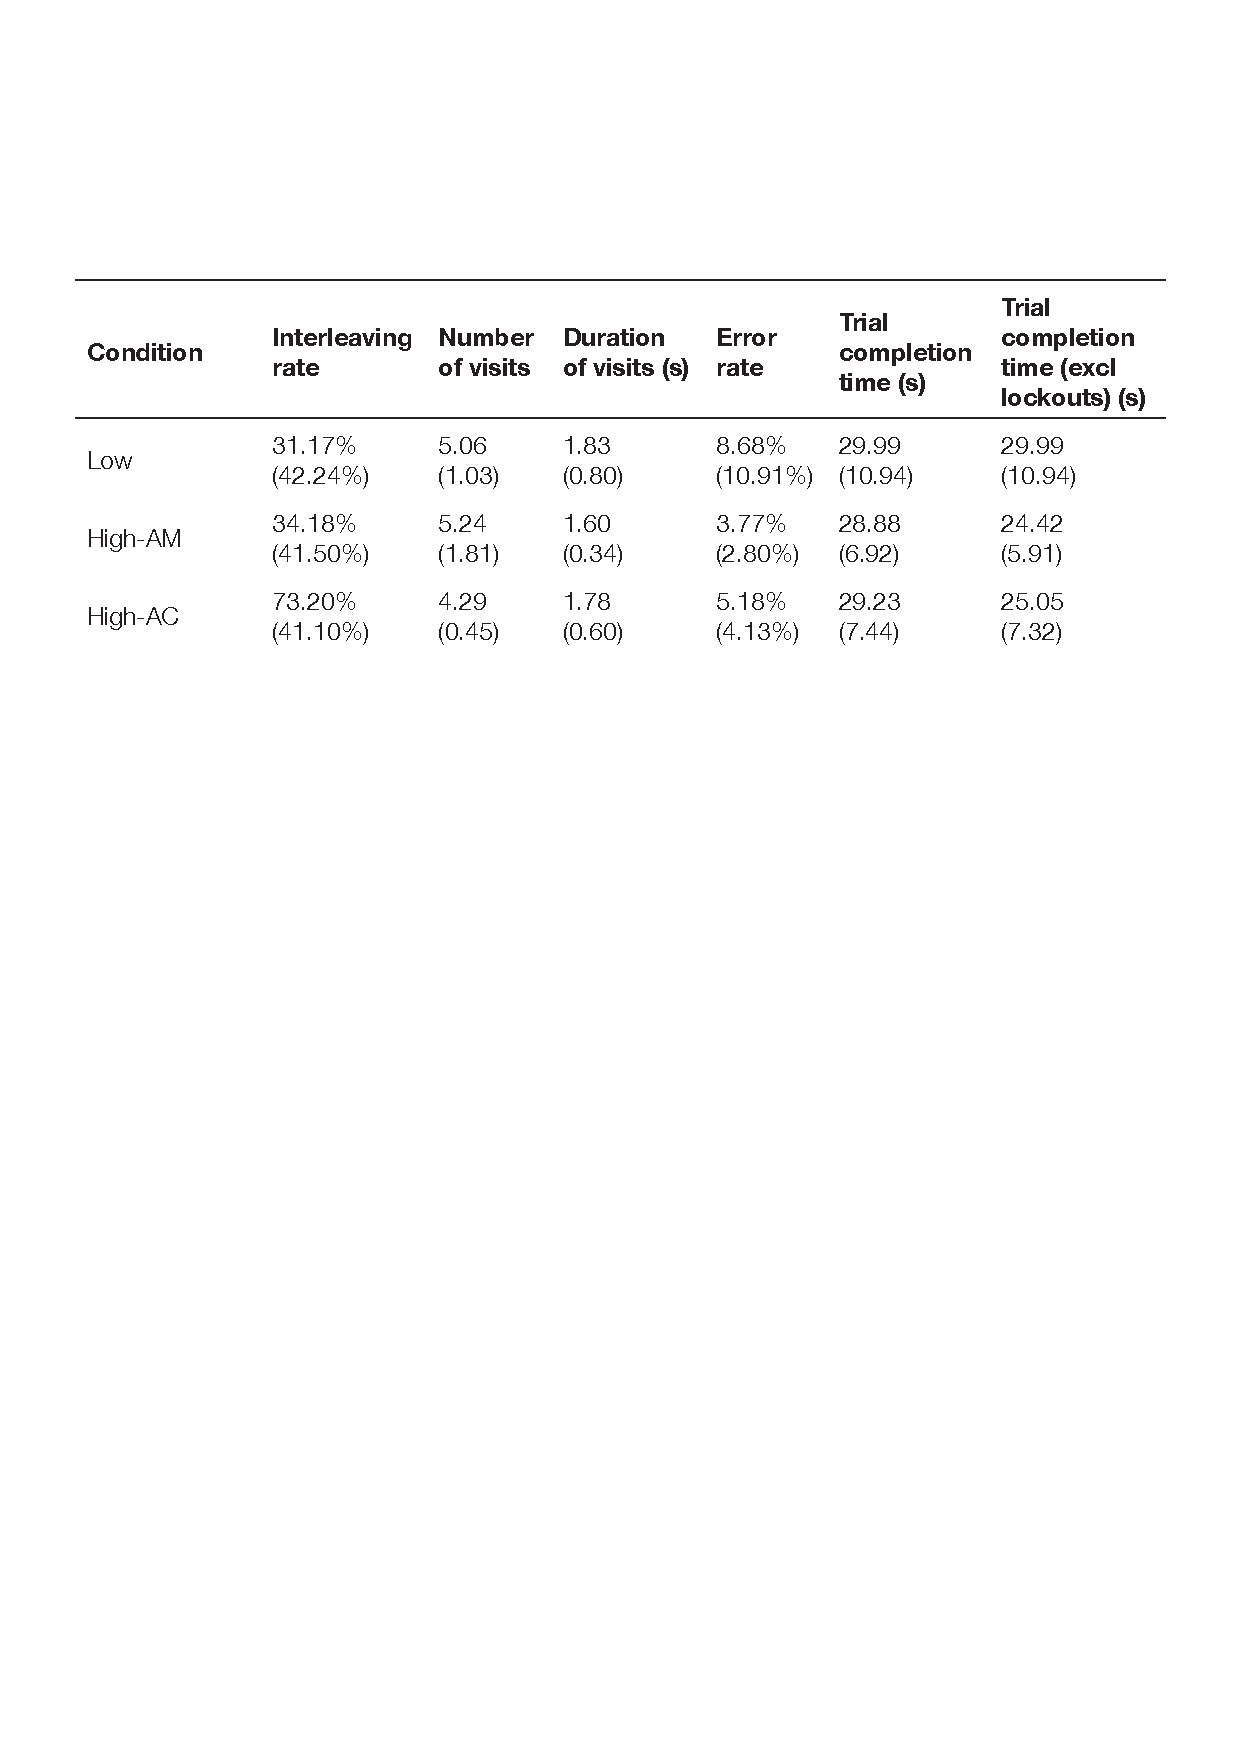
\includegraphics[width=\textwidth]{images/ch34/ch34-4_means.pdf}
\caption[Study 4 means and SDs of dependent measures]{The means (and standard deviations) of all dependent measures for each condition. The rates are calculated by dividing the number of occurrences to the number of opportunities, e.g. an interleaving rate of 50 percent means that on average, a participant interleaved on 50 percent of the trials.}
\label{tbl:ch34_4-means}
\end{table}

\subsubsection{Interleaving strategies}
A trial was labelled as 'interleaving' if the participant started entering one expense but interleaved to the other expense before completing the first one. The interleaving rate for each condition was calculated by dividing the number of trials where people interleaved by the number of total trials.  

Across conditions, most participants were consistent in their strategy choice, and either interleaved between expenses on almost no (0\%) or all (100\%) trials. Because the data was centered around these extreme values, for the interleaving rate the medians are reported in addition to the means, as the medians are more representative of the central tendency of the data.

%There was a significant difference between conditions, $\chi^2$(2) = 6.81, \textit{p} = 0.03, with a mean interleaving rate of 73.2\% (Mdn = 96\%) in the High-AC condition, 34.18\% (Mdn = 12\%) for the High-AM condition, and 31.17\% (Mdn = 6\%) for the Low condition. The boxplots in Figure \ref{fig:ch34_4-boxplots} show the variability of interleaving rates across conditions. 

Participants interleaved most often between expenses in the High-AC condition (\textit{M} = 73.20\%, \textit{SD} = 41.10\%), compared to the Low (\textit{M} = 31.17\%, \textit{SD} = 42.24\%) and High-AM (\textit{M} = 34.18\%, \textit{SD} = 41.5\% ) conditions, $\chi^2$(2) = 6.81, \textit{p} = .03. A post-hoc Dunn's test showed there was a difference between the High-AC condition and the Low (\textit{p} = .02) and the High-AM (\textit{p} = .03) conditions, but not between the Low and High-AM conditions (\textit{p} = .90). The median interleaving rate was 6\% for the Low condition, 12\% for the High-AM condition, and 96\% for the High-AC condition. The boxplots in Figure \ref{fig:ch34_4-boxplots} show the variability of interleaving rates across conditions. 

\begin{figure}
 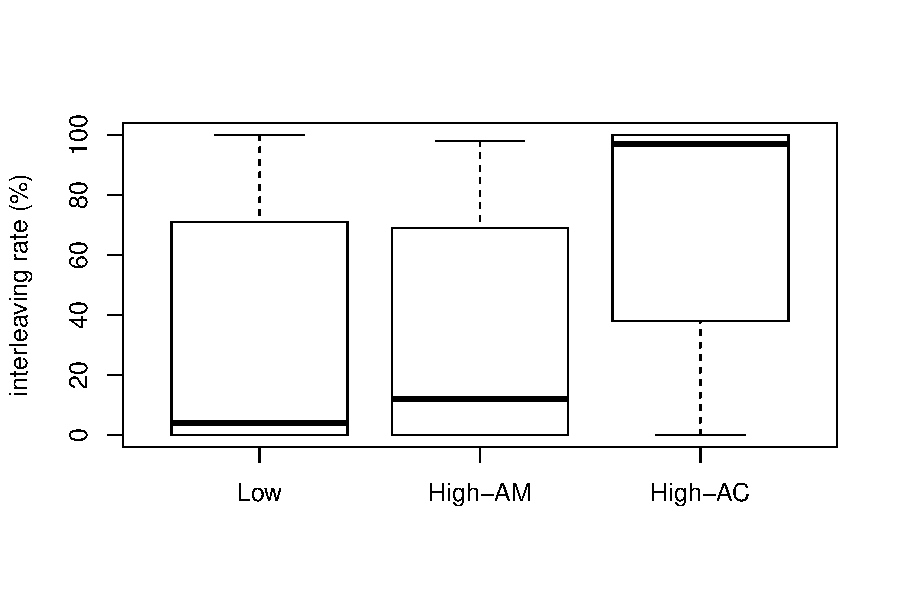
\includegraphics[width=0.6\textwidth]{images/ch34/ch4_4-boxplot.pdf}
\caption[Study 4 boxplot of interleaving rates]{Boxplot of interleaving rates in each condition.}
\label{fig:ch34_4-boxplots}
\end{figure}

Figure \ref{fig:ch34_4-linechart} shows the distribution of interleaving rates for each condition. The lines all have peaks at the left and right end, indicating the interleaving rate was predominantly 0\% or 100\% in each condition. Graphs of each individual participant are included in Appendix \ref{ch:S4_PartPlots}, which shows per trial whether a participant interleaved or not. These graphs further illustrate that participants used the same strategy throughout the experiment.

\begin{figure}
 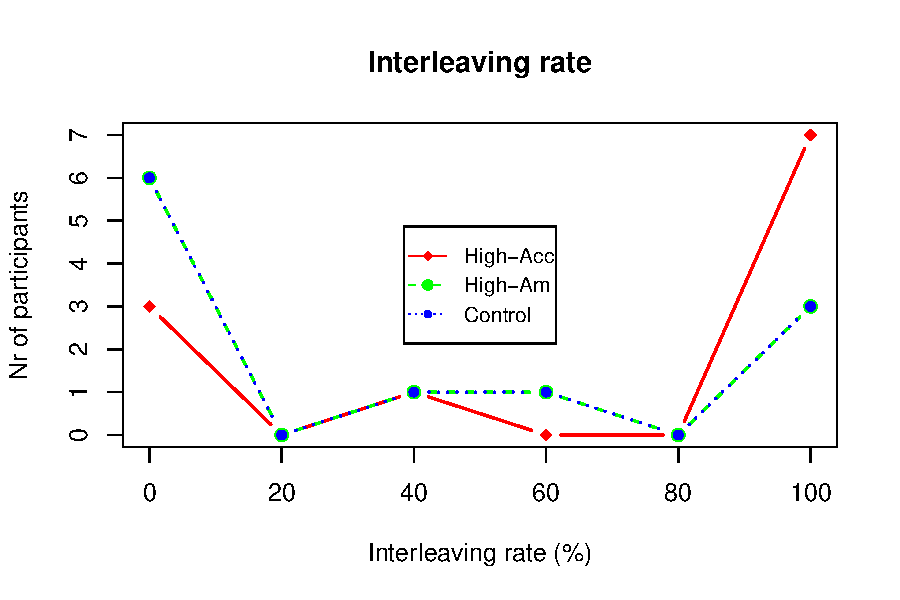
\includegraphics[width=\textwidth]{images/ch34/ch34-4_linechart.pdf}
\caption[Study 4 frequency of interleaving rates]{Line graph showing the frequency of interleaving rates for each condition; the lines of the Low and High-AM condition overlap and follow the same trend. As can be seen, all three lines have two peaks at 0 and 100, which means that most participants interleaved on 0\% or 100\% of all trials.}
\label{fig:ch34_4-linechart}
\end{figure}

\subsubsection{Number and duration of visits}
There was no difference in the number of visits, $\chi^2$(2) = 2.90, \textit{p} = .23. On average, participants made 4 visits per trial (i.e. one visit per data entry). Participants visited an information page for 1.8 seconds on average, and there was no significant difference in duration of visits between conditions, $\chi^2$(2) = 0.30, \textit{p} = .80. 

\subsubsection{Most common order of actions}\label{sec:ch34-StrategyFreq}
To get a better insight in the specific order in which participants viewed and entered items, the trials were grouped based on the order of actions. There were six different possible actions: viewing the amounts window (V-Am), viewing the account codes window (V-Acc), entering the first amount (E-Am1), entering the second amount (E-Am2), entering the first account code (E-Acc1), and entering the second account code (E-Acc2). This iteration of grouping the trials resulted in 12 different strategy groups in total, with the majority of trials (92\%) grouped in the same four groups, which are shown in Figure \ref{fig:ch34_4-groupstr}. In the Low and High-AM conditions, the most common strategy was strategy (a): participants first viewed the Amounts window and entered the amount of the first expense, and then viewed the Account code window and entered the account code of hte first expense, before they visited the Amounts window again to enter the amount of the second expense, and view the Account code window to enter the account code of the second expense. Strategy a is also the strategy used in Figure \ref{fig:ch34_4-tasklayout} to illustrate what the task steps in the task interface look like.

In the High-AC condition, participants predominantly used Strategy (c): they first switched to the Amount window, which had no delay, and entered the amount of the first expense in the data entry form, after which they switched to the Amount window again to view and enter the amount of the second expense. After entering the amounts, they viewed and entered the account codes one-by-one.

Table \ref{tbl:ch34_4-groupstr} shows the frequency with which these strategies were chosen per condition. The most common strategy for each condition are highlighted in bold. The table also shows that even though Strategy (a) and (c) were the most commonly observed strategies, these only accounted for about half of the trials: on the other  trials, participants tried out other strategies.  

%For example, the first strategy (a) shows a strategy where participants started a trial by visiting the Amounts window (Am), and then visiting the Accounts window (Acc). They then entered the account code (Acc1) and the amount (Am1) of the first expense. They then visited the Amounts window again, and entered the amount of the second expense (Am2), and then visited the Accounts window again and entered the account code of the second expense (Acc2). Table \ref{tbl:ch34_4-groupstr} shows the frequency with which these strategies were chosen per condition.

%In the High-Account condition, participants predominantly switched to the page with the Amounts first, which had no delay, and entered these into the data entry form. In the other two conditions, participants mostly entered an amount and account code of the first expense first, and then entered the amount and account code of the second row.

\begin{figure}[!ht]
  \centering
    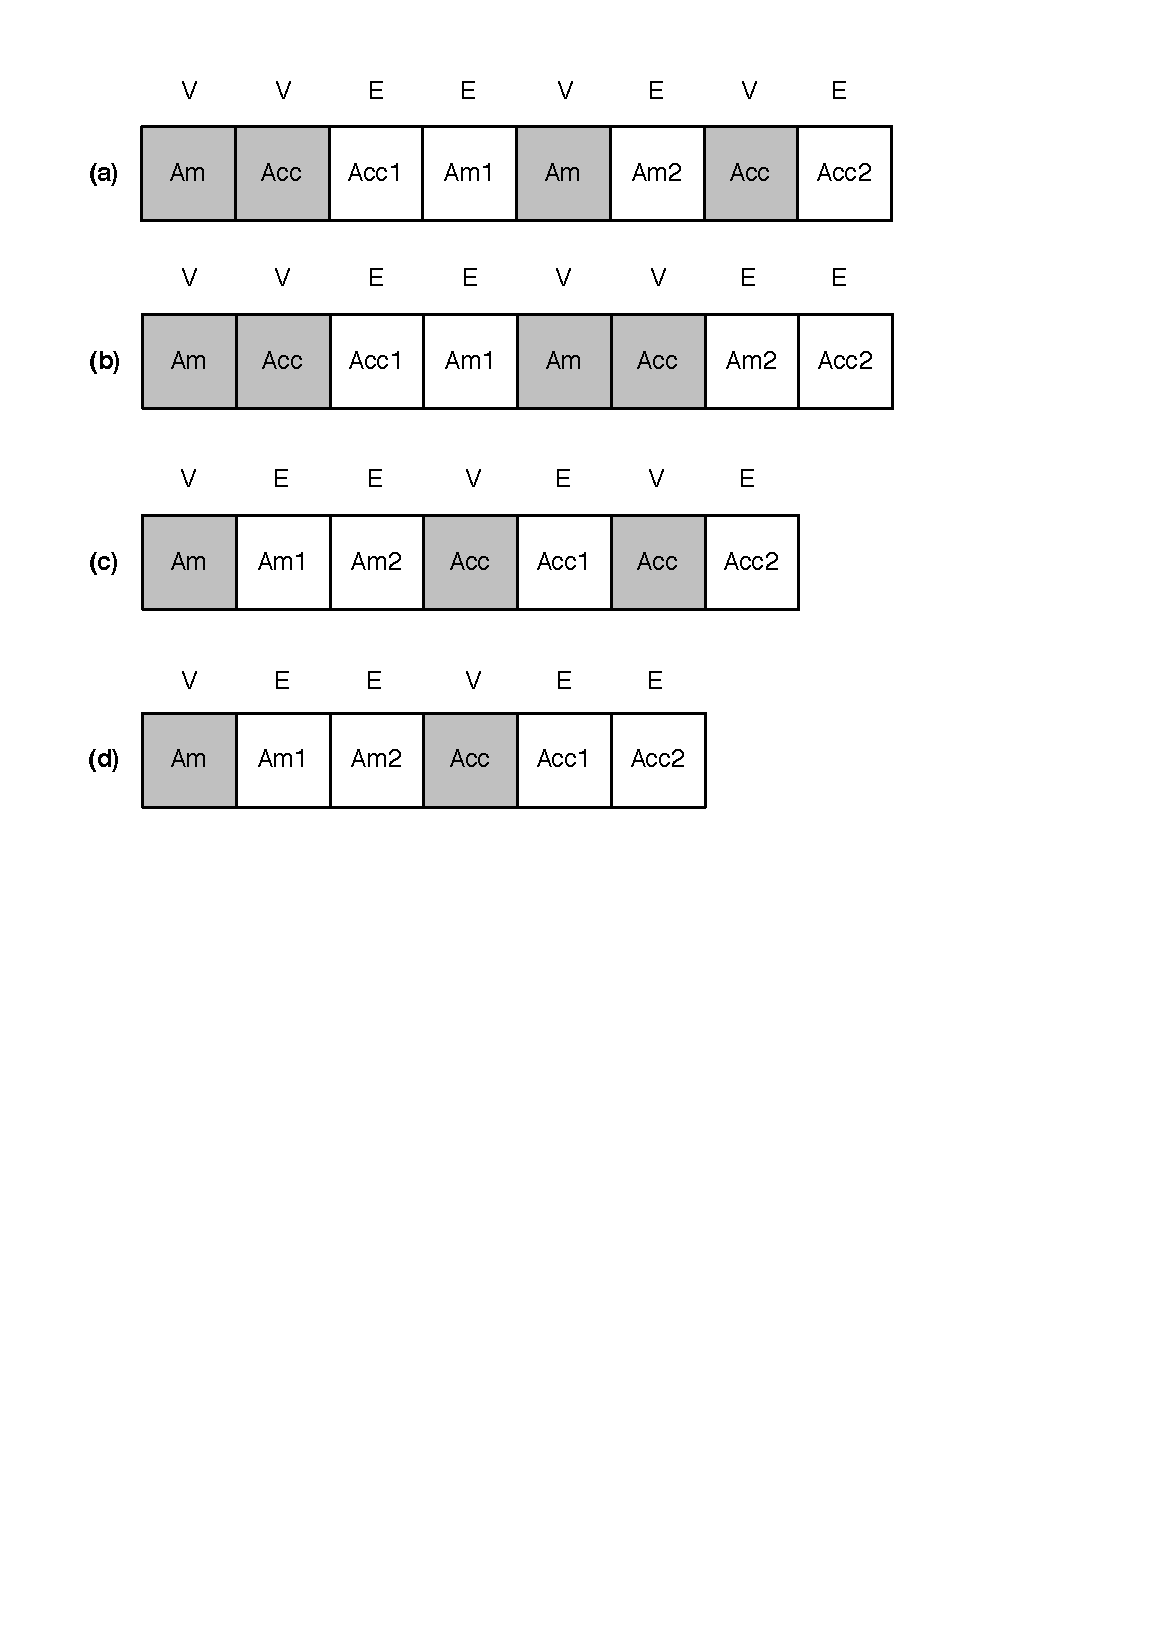
\includegraphics[width=0.5\textwidth]{images/ch34/ch34-4_OrderStrategies.pdf}
      \caption[Study 4 most common order of actions]{The sequence of the most common order of actions. V = visit to an information window, E = entry of a data item. For example, in Strategy (a) a participant first visited the Amounts window, and entered the Amount of the first expense, then visited the Account code window and entered the Account code of the first expense. He/she then viewed the Amounts window again and entered the Amount of the second expense, and then viewed the Accounts window and entered the second expense.}
          \label{fig:ch34_4-groupstr}
\end{figure}

\begin{table}[!ht]
  \centering
    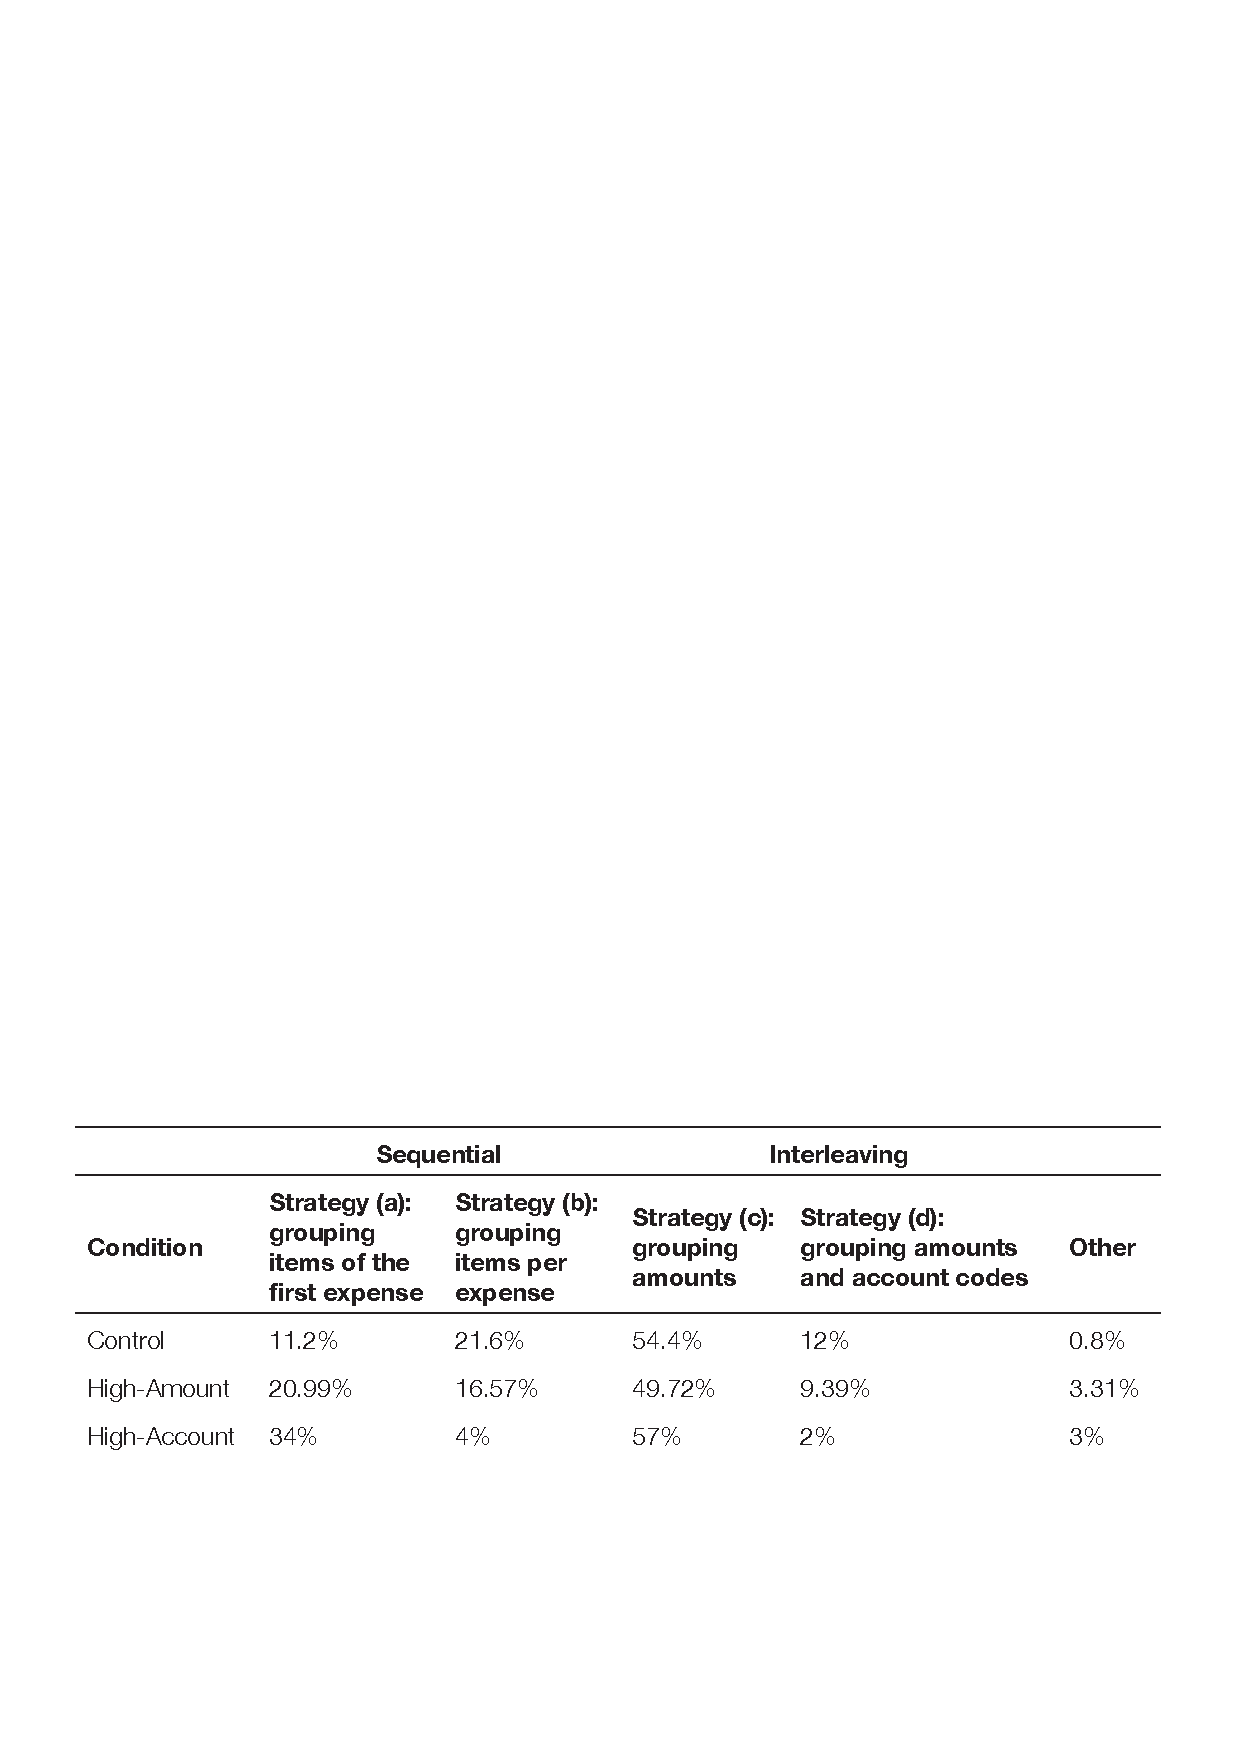
\includegraphics[width=\textwidth]{images/ch34/ch4_4-StrategyFreq.pdf}
\caption[Study 4 occurrence of most common strategies]{The occurrence of the most common strategies per condition; the most common strategy per condition is highlighted in bold. The rates are calculated by dividing the number of occurrences to the number of opportunities, e.g. a  rate of 50 percent means participants used this strategy on 50 percent of the trials. The strategies are shown graphically in Figure \ref{fig:ch34_4-groupstr}.}
          \label{tbl:ch34_4-groupstr}
\end{table}

\subsubsection{Task performance}
The High-Cost conditions had an extra time cost to overall completion time, due to the delay when switching one of the windows. Therefore, two completion times were calculated: one measure considered the actual completion time with the delay times included, and another measure considered the completion time with the delay times removed. Considering these two times, there was no difference in the time it took to complete a trial using the actual completion time,  \textit{F}(2, 30) = 0.16, \textit{p} = .90, or with the delay times removed, \textit{F}(2,30) = 1.63, \textit{p} = .20.

There were 200 data entries, so in total there were 200 opportunities for a participant to make a data entry error. The error rates were calculated as the number of errors divided by the number of entries. Though the mean error rate was higher in the Low condition (M=8.68\%, SD=10.90\%) compared to the High-AM (\textit{M}=3.77\%, \textit{SD}=2.79\%) and High-AC (\textit{M}=5.18\%, \textit{SD}=4.13\%) conditions, this difference was not statistically significant, $\chi^2$(2) = 0.41, \textit{p} = .80. 

%Considering these two times, there was no difference in the time it took to complete a trial using the actual completion time,  $\chi^2$(2) = 0.15, \textit{p} = 0.9, or with the delay times removed,  $\chi^2$(2) = 2.92, \textit{p} = 0.2. On average, with the delay times included, participants took about 29 seconds per trial across conditions.

While the above analysis shows no significant difference in the number of data entry errors, it does not give any indication of the type of errors that were made. Having insight into the type of errors can inform how to design better data entry interfaces to prevent these errors \citep{Wiseman2011}. For example, it has been shown that interleaving between tasks increases the likelihood of omitting task steps \citep{Back2012}. %I was therefore interested to see whether interleaving between expenses increased the number of omission errors. 
The errors were therefore categorised according to type, to see what type of errors were made across conditions. To study the type of errors that were made, \citeauthor{Wiseman2011}'s \citeyearpar{Wiseman2011} taxonomy of number entry errors was used to categorise data entry errors. This taxonomy was originally created by grouping and coding 350 number entry errors gathered during a number entry experiment. As can be seen in Figure \ref{fig:ch34_4-typeoferrors}, the most prominent error types were when participants had a digit(s) wrong (60 times), when a data entry was skipped (75 times) or when they entered a 'wrong' number, which was supposed to be entered in another data entry field (57 times): these types of errors make up for 61\% of all errors. The 'digit(s) wrong' and 'skipped' errors happened more frequently in the Low condition, but there was otherwise no remarkable difference in type of errors between conditions. 

%\citeauthor{Wiseman2011}'s \citeyearpar{Wiseman2011} taxonomy of number entry errors was used to analyse the types of data entry errors that were made. 

\begin{figure}
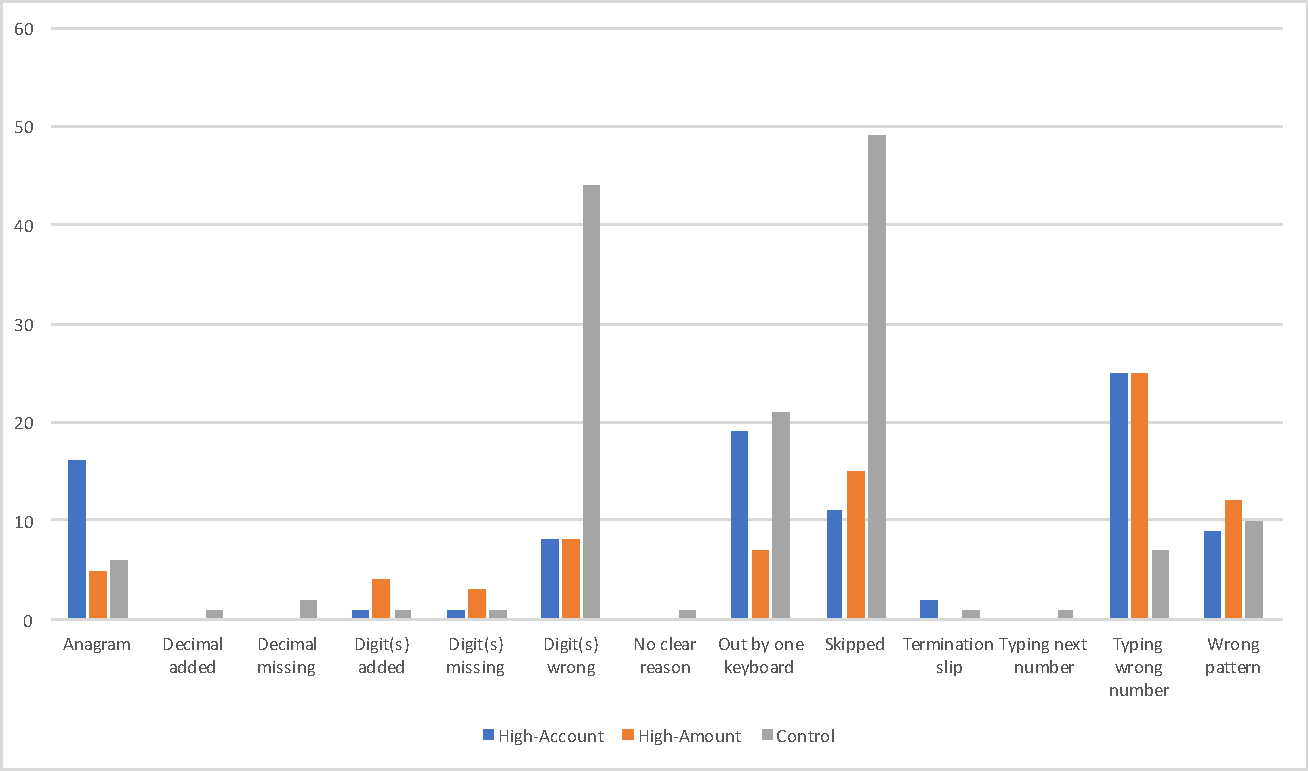
\includegraphics[width=\textwidth]{images/ch34/ch34-4_TypeofErrors.pdf}
    \caption[Study 4 type of data entry errors]{The type of data entry errors made in each condition. The most common error types were when participants had a digit wrong, when a data entry was skipped, or when the wrong number was entered in an input field.}\label{fig:ch34_4-typeoferrors}
\end{figure}

\subsubsection{Qualitative findings}
After the experiment had ended, participants were debriefed and the purpose of the study was explained. Some participants reflected on their strategies and gave additional explanations behind them. While these explanations are not the main focus of analysis and only serve to complement the quantitative measures, it helps understand people's motivation behind some of the measured strategies.

Participants mentioned they adapted their strategy several times throughout the experiment, in order to find the quickest way to complete the task. Because amounts were shorter and easier to remember, five participants mentioned they tried to first view all amounts before entering them. They tried this strategy with account codes as well, but these were longer and therefore it was more difficult to memorise two items at a time. As a result, most participants ended up viewing and entering each account code one by one. This kind of behaviour is illustrated as Strategy (d) in Figure \ref{fig:ch34_4-groupstr}.

Four participants noticed that numbers re-occurred throughout the experiment. They felt it was easier to memorise a number that had already occurred earlier in the experiment, so when a trial contained a number they recognised, they would memorise this item as well as another item, before returning to the entry form. If they did not recognise the number, they would memorise one item. Furthermore, as data items had a fixed length, some participants started a trial by entering placeholders: in the amount data entry field, they placed a number consisting of four digits and a decimal point, and in the account code data entry field a number of six digits was entered. They would then visit the information windows to check which of the digits of the items they needed to change. 

\subsection{Discussion}
%Summary
The aim of this study was to understand the effect of time costs on the timing of inquiries during a data entry task. To address this aim, I created a new experimental task that involved switching between three different windows to look up and enter data. The main findings of Study \hyperref[st:Study4]{4} are:

\begin{itemize}
\item
if there were no differences in time costs, participants completed a data entry sheet in sequential order, and completed one expense before moving to the next one. 
\item
in the High-Cost conditions, people interleaved significantly more between expenses in the High-AC but not High-AM condition. 
\item
participants grouped items in all conditions, and there was no difference in number of visits between conditions.
\end{itemize}

\subsubsection{Timing of inquiries}
The findings partly support the hypothesis that people postpone inquiries with a high time cost, but it does not explain why participants entered the data entry sheet in sequential order in the High-AM condition. 
These results can be explained when considering the order in which the data was presented, and the order in which items were entered. Across conditions, participants predominantly started each trial by entering the first cell of the data entry sheet, the amount of the first expense, regardless of whether the Amounts window had a 2-s time cost or not. However, the second item they entered was dependent upon which window had a time cost: if the Amounts window had a time cost, participants would enter an account code next. If there was a time cost when switching to the Account codes window, they would enter the second amount next.
This behaviour suggests that time costs do not influence the first visit, but do affect subsequent visits. Even though the time cost was consistent throughout the experiment, potentially the experiment was too short for participants to learn which of the windows had a delay and only adapted their strategy after they had already entered the first item. Furthermore, participants tended to stick to the same strategy they had started with throughout the experiment.

The finding that participants postpone inquiries with a high time cost is consistent with findings from Study 2 and suggests people schedule their inquiries more efficiently and effectively. Though there was no measured difference in task performance in the study, long interruptions have been shown to be more disruptive than short ones \citep{Altmann2017, Monk2008}, and leaving these until a natural breakpoint can reduce errors, as it is easier to resume a task \citep{Gould2013a, Iqbal2005}.

\subsubsection{Chunking of data items}
In contrast with Study \hyperref[st:Study3]{3} and prior work \citep{Gray2006}, an increase in time costs did not reduce the number of visits. However, in prior studies there was no interaction involved to view information in the Low-Cost condition: information was permanently visible in the task interface. In the current study, participants always had to move their mouse and click in order to view the information pages, which may have encouraged them to try and reduce visits and chunk items even in the Low condition. The time cost affected which items participants chunked together, but not whether they chunked items or not.

\subsubsection{Transfer of strategies}
People adapted their strategies even if only some, but not all, of the information was hard to access. Exposure to time costs may have made people adapt their strategies for all inquiries. This transfer of strategies is consistent with previous research, that has shown a more memory-based strategy can be trained and transferred to other situations where the cost to access information is no longer high \citep{Patrick2014}. This study extends these findings by showing that inquiry strategies can also transfer within a task, when the user has to access multiple information sources with both a low and high time cost.

\subsubsection{Limitations}
%The study has two limitations regarding the type of data items used, and the order of data.

%Order
%All conditions had the same order in which data was presented on the data entry sheet, as well as the same order in which the windows were shown in the top menu. 
The results suggest that the order in which data was presented may have influenced the order in which people entered data: across all conditions, participants mostly started a task by entering the first data item. An increased time cost affected subsequent items that were entered after the first item. Future studies could be done to investigate whether changing the order has an effect on people's inquiry strategies.

% As the results show, the effect of time costs was only shown in the High-Account condition, which may have partly been caused because of a difference in data item: account codes were longer and more difficult to memorise, which may have been an additional time cost, that encouraged people to first look up amounts.

\subsection{Conclusion}
Taken together, we learn from this study that people avoid time costs by postponing some inquiries with an increased time cost, and addressing inquiries with a low time cost first. In contrast, if all inquiries have the same time cost, participants predominantly filled in a data entry sheet in sequential order. They completed in one expense first, before moving to the next one. 

In the current study, both expenses were shown in the same window. Even though switching between expenses was labelled as an 'interleaving' strategy in the study, the expenses were part of one form, and could be seen as part of the same task. What we do not know from Study \hyperref[st:Study4]{4} is whether participants will also avoid time costs of inquiries by interleaving between two data entry tasks separated over two different windows. Based on the results of the current study, the hypothesis is made that a difference in time costs makes people more likely to interleave between different data entry tasks to enter items with a low time cost first. This hypothesis is tested in Study \hyperref[st:Study5]{5}.

%The aim of this study was to investigate the effect of time costs on the number, duration and timing of inquiries from multiple sources. We learn from this study that people avoid time costs by postponing some inquiries with an increased time cost. If there were no differences in time costs, people completed a data entry sheet in sequential order, and completed one expense before moving to the next one. 

%In this study, both expenses were shown on the same window, and could be seen as part of the same task. 

\section{Study 5: Inquiries for multiple tasks}\label{st:Study5}
\subsection{Introduction}
So far, Study \hyperref[st:Study3]{3} has shown that people avoid time costs by reducing the number of inquiries, and Study \hyperref[st:Study4]{4} suggested that people avoid time costs by postponing inquiries with a high time cost. In these studies, people were only presented with one task at a time. Workers in Study \hyperref[st:Study2]{2} often dealt with several data entry tasks and windows at a time, and had to be careful not to enter information in the wrong windows. How would people deal with time costs when they have to coordinate multiple tasks? Participants in Study \hyperref[st:Study1]{1} and \hyperref[st:Study2]{2} avoided switches to tasks that were completely unrelated to their data entry work, but people may switch between similar data entry tasks if it makes them faster. For instance, upon opening a spreadsheet that takes time to retrieve, it may be more efficient to enter the account codes from that spreadsheet for multiple tasks. However, multitasking can also be prone to errors \citep{Carrier2015}.

Prior research, studying the effect of time costs on multitasking in a hospital setting, found that increased time costs reduces multitasking. \citet{Back2012} conducted a lab experiment where participants had to enter information from a prescription form into two simulated infusion pumps. For each pump, they had to enter two types of information: the medication dose and the time duration. If the form was physically further away from the pumps, participants more often completed one pump before starting another and as a result made fewer errors in omitting a task step. The higher access cost had the effect that participants memorised and chunked information on the form according to the pump rather than type of information, which reduced multitasking.

However, in Back et al.'s study, all information was located on one information source, and participants incurred a single cost to access it. People therefore chunked information to memorise as much information per visit as possible, so that they did not have to revisit the source too often. It is unclear what the effect of time costs is in scenarios where people do not have to get multiple information items from one source, but rather information from multiple sources. How do people prioritise which information to look up first? Do they still complete looking up information for one task first, before starting another task?

The aim of Study \hyperref[st:Study5]{5} is to test whether the effect of time costs, as found in Study \hyperref[st:Study4]{4}, extend to a multi-task setup. Participants were asked to complete an experiment similar to the task in Study \hyperref[st:Study4]{4}, but had to complete two (of the same) data entry tasks per trial. The hypothesis is:

\begin{itemize}
\item [H1.]
Participants in the Low condition will enter items from one data entry task first, before entering the second task. Participants in the High-Cost conditions will enter the Low-Cost items first, and postpone entering the High-Cost items.
\end{itemize}

\subsection{Method}
\subsubsection{Participants}
Thirty-nine participants (32 female, seven male), ranging from 18-46 years (M = 25, SD= 8) took part in the experiment. They were recruited from a university subject pool and received $\pounds$4 for their participation.

\subsubsection{Materials}
The task was similar to the one used in Study \hyperref[st:Study4]{4} but differed in one aspect. Instead of filling in one data entry form per trial, participants had to complete two sheets per trial, which were shown on two different windows (see Figure \ref{fig:ch34_5-tasklayout}). Each data entry sheet contained one expense, and participants completed the trial by entering the amount and account code for each sheet. The aim of this follow-up study was to investigate if differences in time costs of the two information windows makes people more likely to interleave between two separate data entry tasks.

\begin{figure}
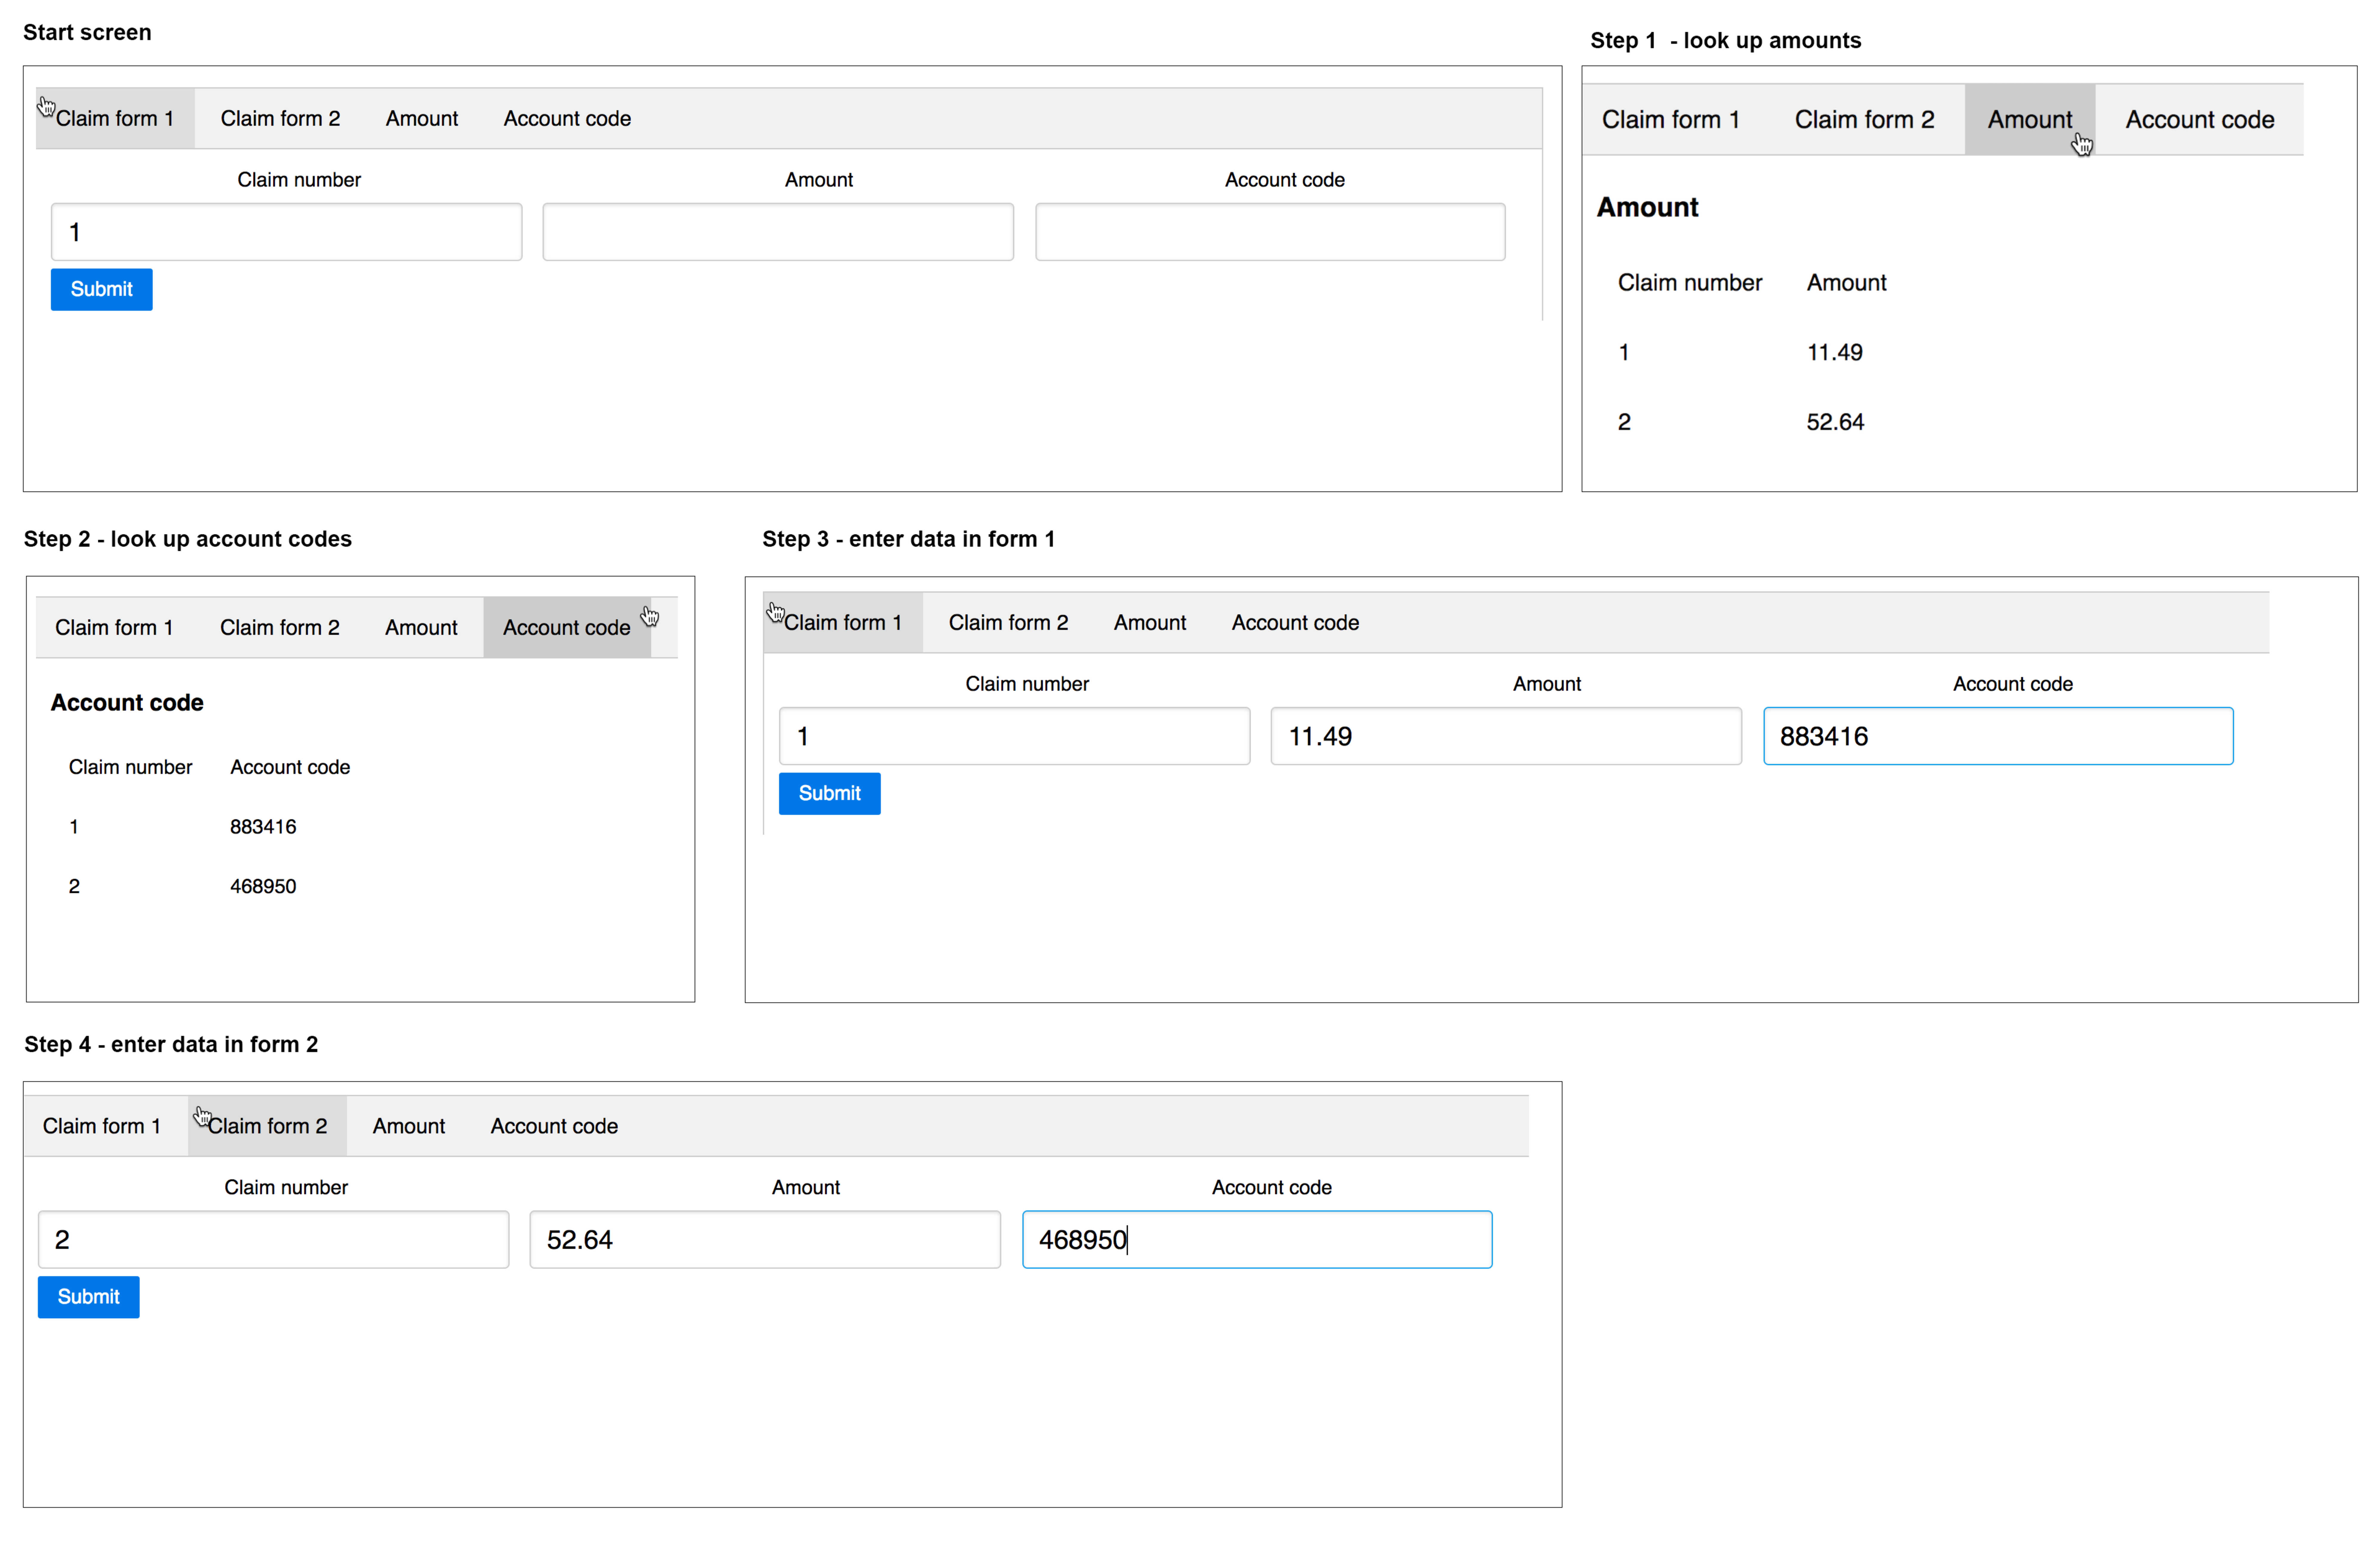
\includegraphics[width=\textwidth]{images/ch34/ch34-5_Tasksequence.pdf}
    \caption[Study 5 data entry task layout]{Participants had to enter two data entry tasks per trial, each containing two items. Each trial started by showing the first data entry form. As in Study 4, the data items for both tasks were retrieved from a separate Amounts window (Step 1) and entering the items for the first expense (Step 2), and the second expense (Step 3). Participants had to repeat Steps 2 and 3 for the account codes, before submitting the data entries and moving on to the next trial. The participant could switch back and forth between windows as often as is needed}\label{fig:ch34_5-tasklayout}
\end{figure}

\subsubsection{Design}
The experiment was a between-participants design with the presence of a delay as the independent variable. 
As in Study \hyperref[st:Study4]{4}, in the \textit{Low-Amount, Low-Account} (Low) condition, there were no delays in opening any of the windows. In the \textit{High-Amount, Low-Account} (High-AM) condition, there was a 2-s delay when opening the Amount window, and no delay when opening the Account window. In the \textit{Low-Amount, High-Account} (High-AC) condition, there was no delay when opening the Amount window, and a 2-s delay when opening the Account window. There were no delays in opening the data entry form in any of the conditions 
The main dependent variable was whether participants interleaved between sheets or not: did participants enter the data items in sequential order, or did they interleave between the two sheets? If participants entered the amount and account code of one sheet before entering the other sheet, this was considered a sequential order. If participants entered amounts of each sheet first, followed by entering the account codes or vice versa, this was considered interleaving. All window switches and key presses were recorded to determine in which order data was entered. Window switches were recorded to capture when and how often a participant looked up the data items. Other dependent variables were trial completion time, data entry error rate, and type of errors.

%As in Study 4, in the Control condition there were no delays in opening the windows. In the High-Amount condition, there was a delay in opening the window with amounts. In the High-Account condition, there was a delay in opening the window with account codes. 

\subsubsection{Procedure}
The experimental setup was similar to Study \hyperref[st:Study4]{4}. For each experimental trial, participants had to enter four data items: they had to complete two forms with two entries each, an account code and an amount. For each experimental trial, participants had to enter four data items, two for each sheet. It was explained that they could use any strategy they wanted, but that it was important to complete both sheets before continuing to the next trial. Participants first completed two practice trials to familiarise themselves with the task, and data from the practice trials were excluded from the analysis. The experiment took approximately 30 minutes.

\subsubsection{Data analysis}
%Participants again predominantly started a trial by viewing and entering the amount of the first expense. If the participant then proceeded to view and enter the account code, this strategy was labelled as a sequential strategy. If the participant proceeded to enter, or view and enter, the amount of the second expense, the trial was labelled as an interleaving strategy. 
The main interest of Study \hyperref[st:Study5]{5} was to see whether people interleaved between tasks or not, and not the specific order of individual actions (e.g. did participants enter multiple items after a single visit to a data window). Strategies are therefore not presented here in the same detail as in Study \hyperref[st:Study4]{4} (see section \ref{sec:ch34-StrategyFreq}). Trials were categorised into an interleaving or sequential category. On a trial-by-trial basis, it was also considered whether people started the trial by visiting and entering a High-Cost or Low-Cost data item.

\subsection{Results}
Table \ref{tbl:ch34_5-means} shows a summary of the results of all three conditions for the dependent variables. Kruskal-Wallis tests were carried out to test if there were significant differences in interleaving rate, number and duration of visits, and error rate between the conditions, as these measures did not follow a normal distribution. 
A Shapiro-Wilk test suggested that the trial completion times did follow a normal distribution, \textit{W} = 0.94, \textit{p} = .05, so a one-way ANOVA was used to test any differences in trial completion time. A p-value of 0.05 was used for assessing the significance of all statistical tests. 

\subsubsection{Cleaning up the data}
Three participants were removed from the data due to extreme values on performance measures.
P28 and P23 made at least one error on every trial. They made 118 and 153 errors out of 200 error opportunities, respectively. P26's session was terminated before the end had been reached, as 45 minutes had passed. This participant spent on average 65 seconds per trial, which is twice as long as the mean trial time of other participants.

These three participants were considered outliers and did not seem to engage with the study, and their data was removed from the dataset. Data of the remaining 39 participants was taken into the data analysis.

\begin{table}
 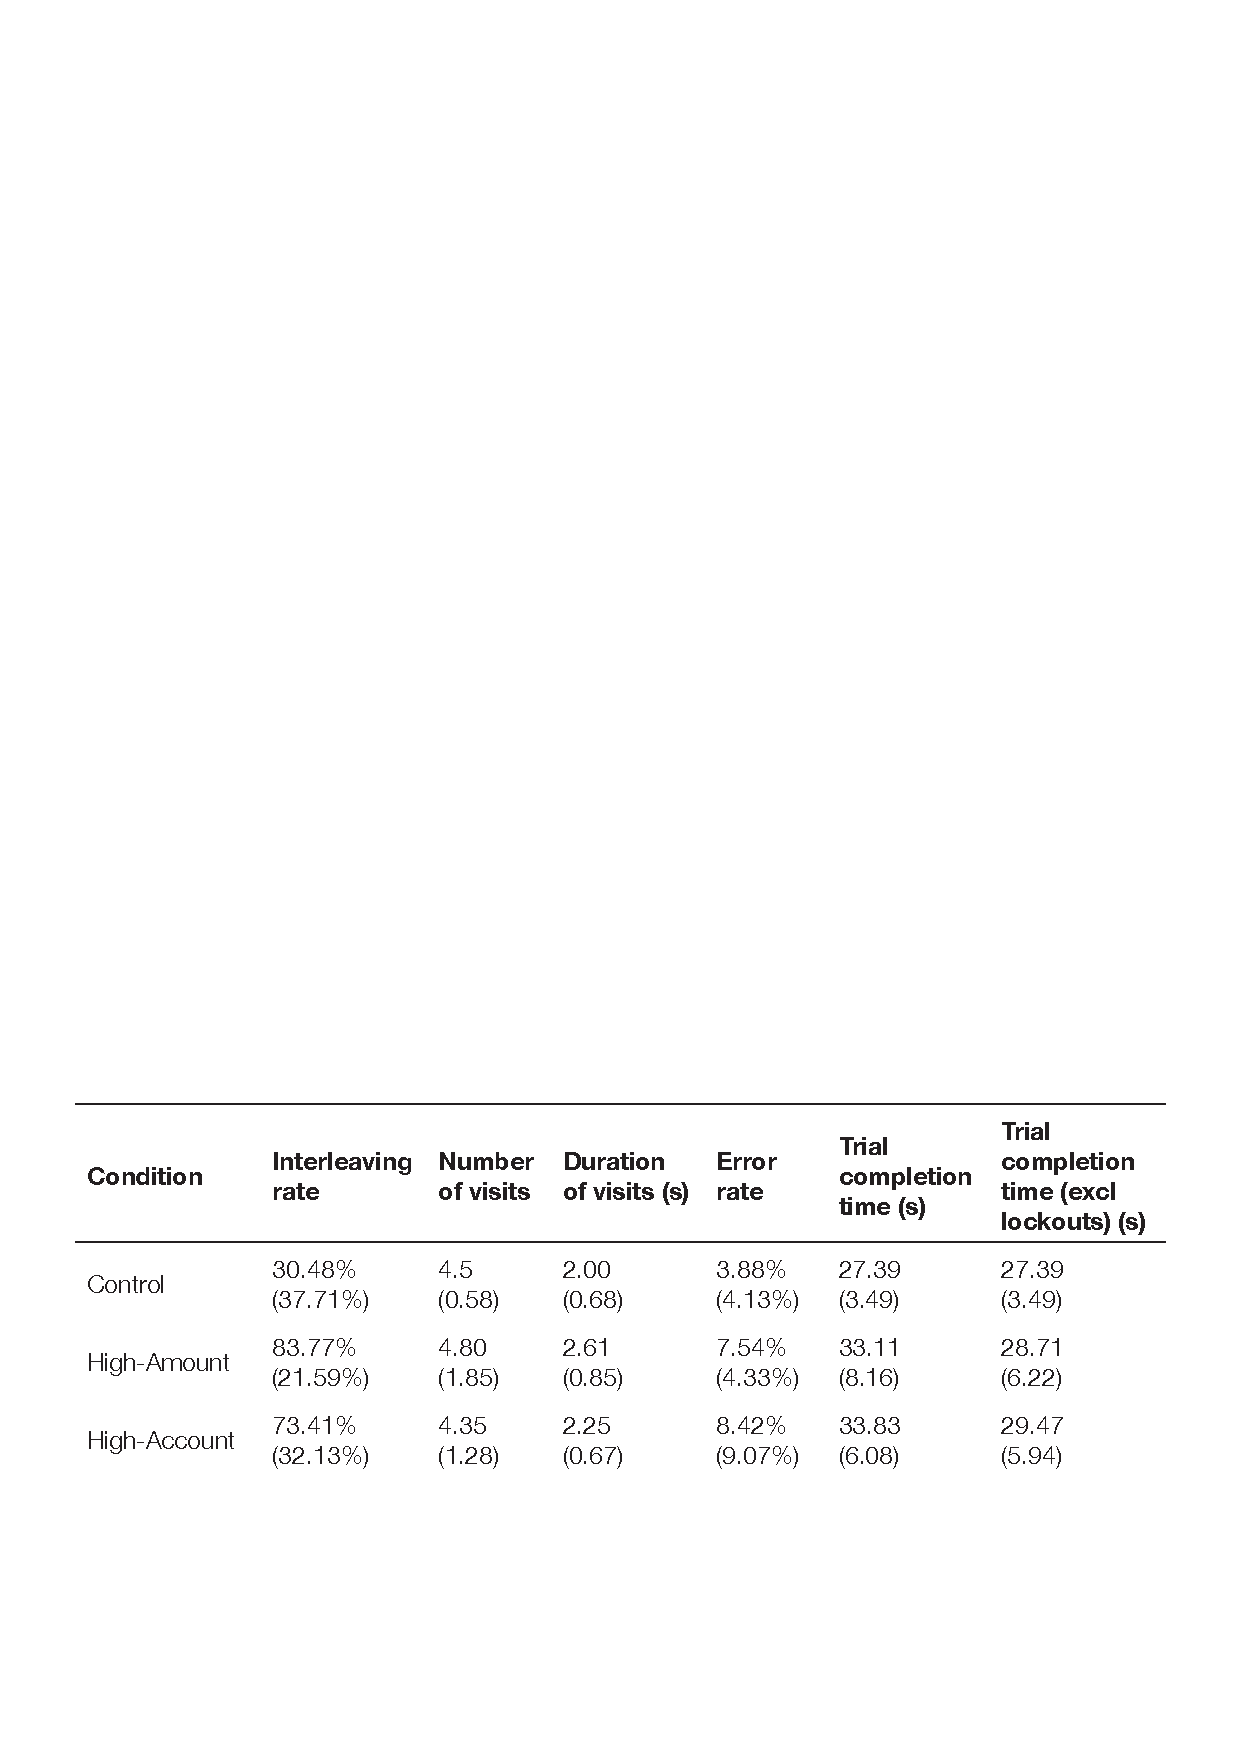
\includegraphics[width=\textwidth]{images/ch34/ch34_5-means.pdf}
\caption[Study 5 means and SDs of dependent measures]{The means (and standard deviations) of all dependent measures for each condition. The rates are calculated by dividing the number of occurrences to the number of opportunities, e.g. an interleaving rate of 50 percent means participants interleaved on 50 percent of trials.}
\label{tbl:ch34_5-means}
\end{table}

\subsubsection{Interleaving strategies}
A trial was labelled as 'interleaving' if the participant started entering one data entry sheet, but interleaved to entering items on the other sheet before completing the first one. The interleaving rate for each condition was calculated by dividing the number of trials where people interleaved by the number of total trials. 

Participants interleaved most often between data entry sheets in the High-AC (\textit{M} = 73.41\%, \textit{SD} = 32.13\%) and High-AM (\textit{M} = 83.77\%, \textit{SD} = 21.59\% ) conditions compared to the Low (\textit{M} = 30.48\%, \textit{SD} = 37.71\%) condition, $\chi^2$(2) = 11.13, \textit{p} < .01. A post-hoc comparison showed there was a difference between the Low and the High-AM (\textit{p} < .01) and High-AC (\textit{p} = .01) conditions, and no difference between the High-AC condition and the High-AM (\textit{p} = .40) conditions. The median interleaving rate was 14.58\% for the Low condition, 94.00\% for the High-AM condition, and 89.58\% for the High-AC condition. The boxplots in Figure \ref{fig:ch34_5-boxplots} show the variability of interleaving rates across conditions. 

As can be seen in Figure \ref{fig:ch34_5-linechart}, which shows the distribution of interleaving rates, all participants in the High-Cost conditions interleaved on at least a part of the trials: the lines of the High-Cost conditions have a frequency of 0 (participants) at an interleaving rate of 0\%. The Low condition has a flat line with no peaks, indicating that interleaving rates in this condition were evenly distributed: participants interleaved on zero, a portion, as well as all of the trials.

\begin{figure}
 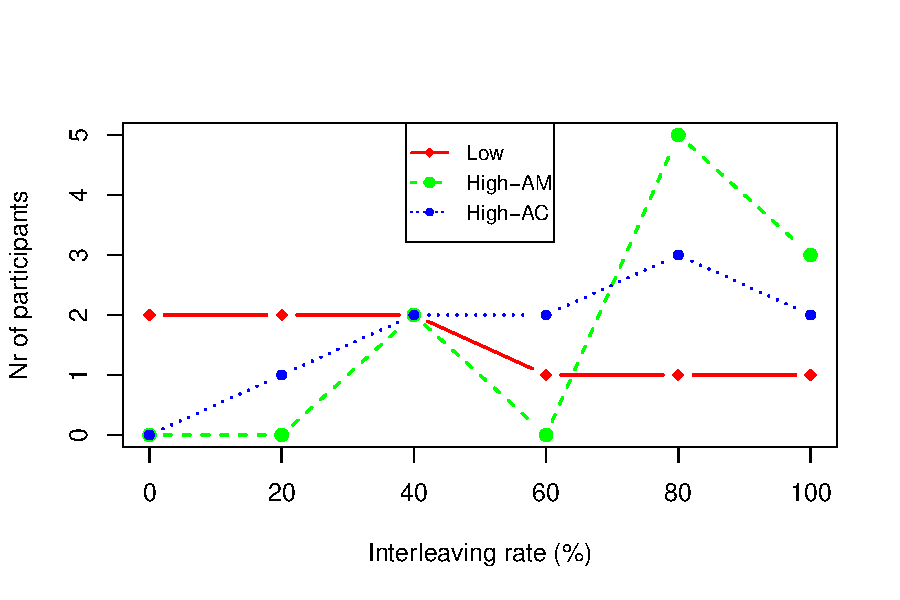
\includegraphics[width=\textwidth]{images/ch34/ch34-5_linechart.pdf}
\caption[Study 5 frequency of interleaving rates]{Line graph showing the frequency of interleaving rates for each condition. It can be seen that in the Low condition, the line is even, which means that an even distribution of participants interleaved on all, a portion, or all trials. The lines of the High-Cost conditions peak at the right end, which means most participants in these conditions interleaved on at least a portion if not 100\% of all trials.}
\label{fig:ch34_5-linechart}
\end{figure}

On the majority of trials (81.95\%) where participants interleaved, they visited and entered Low-Cost items first. On a small subset of trials, participants interleaved by entering High-Cost items first: 2.77\% of these trials occurred in the High-AC condition, meaning participants entered account codes first, and 15.28\% of these trials happened in the High-AM condition, which means participants entered amounts first. 

\begin{figure}
 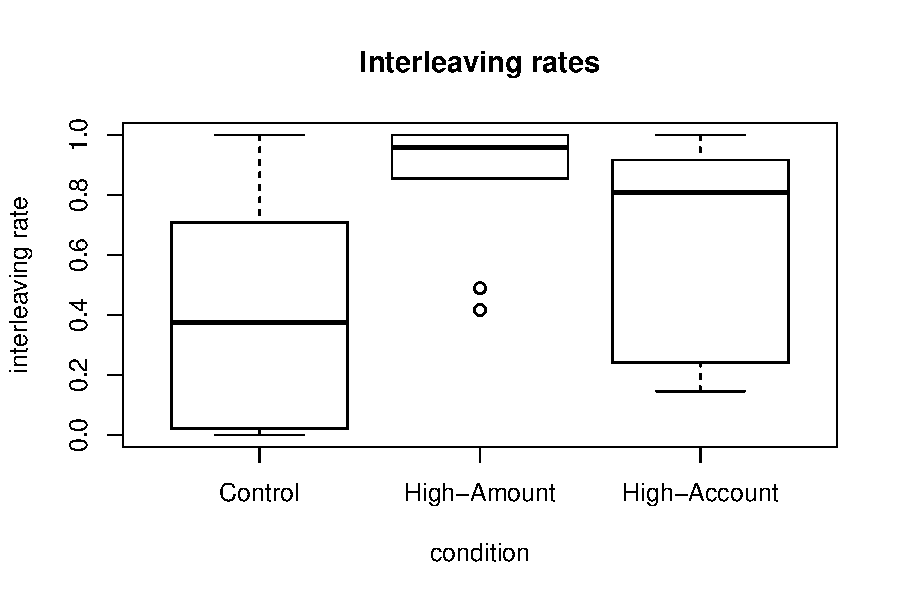
\includegraphics[width=0.6\textwidth]{images/ch34/ch4_5-boxplot.pdf}
\caption[Study 5 boxplot of interleaving rates]{Boxplot of interleaving rates in each condition.}
\label{fig:ch34_5-boxplots}
\end{figure}

\subsubsection{Number and duration of visits}
As in Study \hyperref[st:Study4]{4}, participants made on average four visits per trial, i.e. one visit per data entry. There was no difference in the number of visits, $\chi^2$(2) = 1.59, \textit{p} = .50. Participants made significantly shorter visits in the Low (\textit{M} = 2.00s, \textit{SD} = 0.68s) condition compared to the High-AC condition (\textit{M} = 2.25s, \textit{SD} = 0.67s) compared to the High-AM (\textit{M} = 2.61s, \textit{SD} = 0.85s) and  $\chi^2$(2) = 6.14, \textit{p} = .04. Post-hoc comparisons found a significant difference between  the High-AM and the Low (\textit{p} = .02) conditions, but not between High-AC and Low conditions (\textit{p} = .20) or the High-AC and the High-AM (\textit{p} = .20).

\subsubsection{Task performance}
Two completion times were calculated: one measure considered the actual completion time with the delay times included, and another measure considered the completion time with the delay times removed. When comparing the actual completion time including lockouts, participants were significantly faster in the Low condition (\textit{M} = 27.39, \textit{SD} = 3.49s) than the High-AC (\textit{M} = 33.83s, \textit{SD} = 6.08s) or High-AM (\textit{M} = 33.11s, \textit{SD} = 8.16s) conditions, \textit{F}(2, 36) = 6.73, \textit{p} < .01. With the lockout times removed, the difference is no longer significant, \textit{F}(2, 36) = 0.66, \textit{p} = .50.

There were 200 data entries, so in total there were 200 opportunities for a participant to make a data entry error. The error rates were calculated as the number of errors divided by the number of entries. There was a marginal though not significant effect of time cost on error rate, $\chi^2$(2) = 5.37, \textit{p} = .06. The mean error rate was marginally higher in the High-AC condition (\textit{M}= 8.42\%, \textit{SD} = 9.08\%) compared with the High-AM (\textit{M}=7.54\%, \textit{SD}=4.33\%) and Low (\textit{M} = 3.88\%, \textit{SD} = 4.13\%) conditions. 

%When comparing the actual completion time including lockouts, participants were significantly faster in the Low condition (\textit{M} = 27.39, \textit{SD} = 3.49s) than the High-AC (\textit{M} = 33.83s, \textit{SD} = 6.08s) or High-AM (\textit{M} = 33.11s, \textit{SD} = 8.16s) conditions,  $\chi^2$(2) = 8.52, \textit{p} = 0.01. With the lockout times removed, the difference is no longer significant, $\chi^2$(2) = 1.61, \textit{p} = 0.4.

The type of errors can be seen in Figure \ref{fig:ch34_5-typeoferrors}. The most common error type was when a data entry was skipped: this happened 243 times. %Table 1 shows the number of skipped errors for each condition. 
In the Low condition this type of error occurred 16 times. The error happened more frequently in the High-Cost conditions: in the High-AC condition it happened 114 times, and in the High-AM condition it happened 116 times.
Typing the correct number but in the wrong field happened 78 times. This happened 18 times in the Low condition, 14 times in the High-AC and 46 times in the High-AM condition.
When comparing across conditions, these types of errors happened on a significantly higher proportion of data entries in the High-AC (\textit{M} = 4.58\%, \textit{SD} = 3.6\%) and High-AM (\textit{M} = 6.54\%, \textit{SD} = 5.01\%) compared with the Low condition (\textit{M} = 1.23\%, \textit{SD} = 1.82\%),  $\chi^2$(2) = 11.29, \textit{p} < .01.  A post-hoc comparison showed there was a difference between the Low and the High-AM (\textit{p} < .01) and High-AC (\textit{p} = .01) conditions, and no difference between the High-AC condition and the High-AM (\textit{p} = .40) conditions.

\begin{figure}
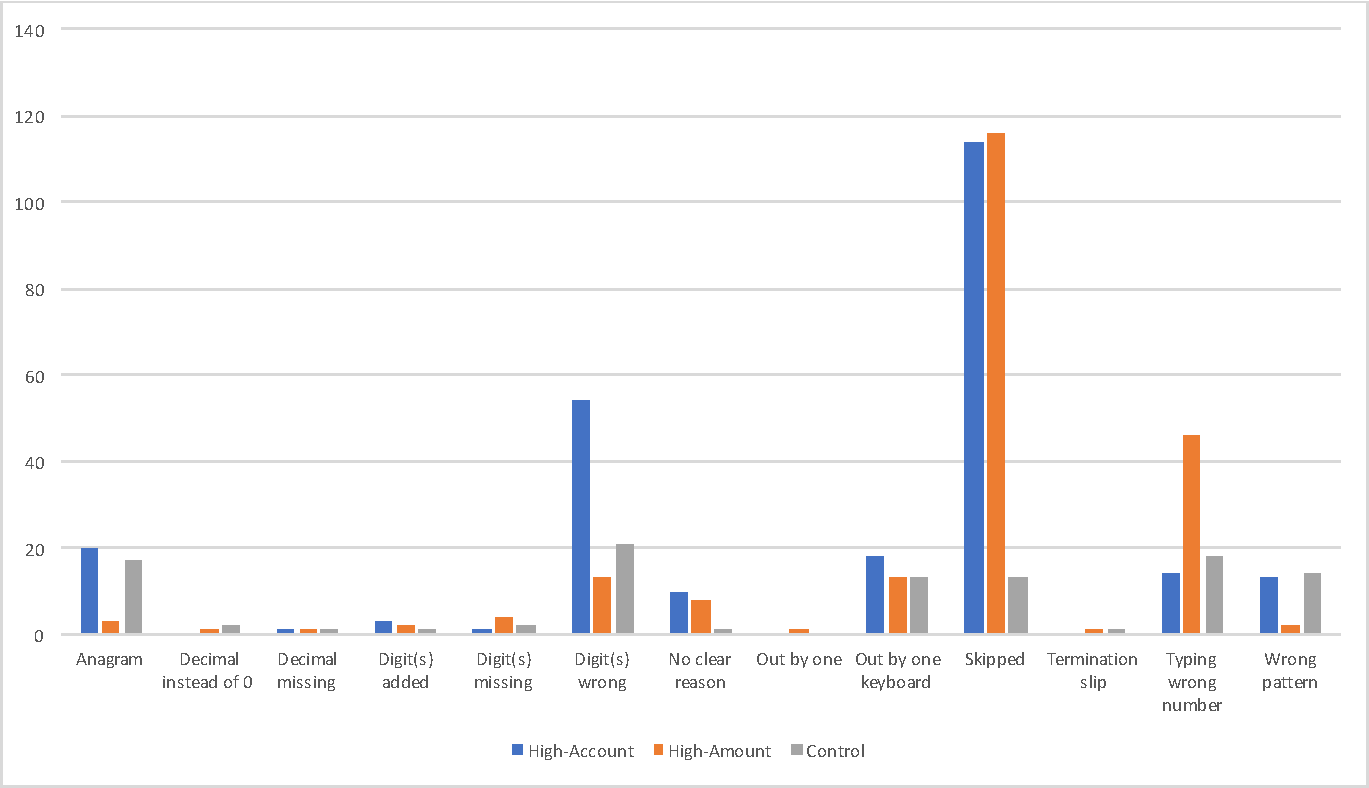
\includegraphics[width=\textwidth]{images/ch34/ch34-5_TypeofErrors.pdf}
    \caption[Study 5 type of data entry errors]{The type of data entry errors made in each condition. It can be seen that skipped errors occurred more often in the High-Cost conditions, in which people interleaved more often.}\label{fig:ch34_5-typeoferrors}
\end{figure}

\subsection{Discussion}
%Effect of time costs
The results show that participants in High-Cost conditions interleaved more between expenses, and made more omission errors, which means a data entry was skipped. The study further supports the notion that people avoid time costs and try to minimise time by postponing some inquiries with an increased time cost, and it demonstrates that this effect of time costs extends beyond a single task setup.
%Though interleaving also happened in the Control condition, it happened significantly more often in the High-Cost conditions. 

The results provide support for the hypothesis that participants in High-Cost conditions enter Low-Cost items of each expense first, and postpone entering the High-Cost items. On a small subset of trials, participants interleaved but instead of entering Low-Cost items, chose to enter High-Cost items first. One explanation for this behaviour is the order in which data was presented, which was briefly discussed earlier in Study \hyperref[st:Study4]{4}. In the High-AM condition, participants may at times have chosen to start a trial by viewing and entering the first data item, which was the amount of the first expense, even though there was a time cost of accessing this item. Another possible explanation is that participants were trying out different strategies, to learn the most efficient strategy for them. 

%avoided time costs by entering items with a low cost first, which meant they interleaved between expenses and entered items of each expense that had a low cost first. 

The finding that people increase their interleaving behaviour to avoid time costs is consistent with the soft constraints hypothesis that people adapt their strategies to millisecond changes in an interface \citep{Charman2003, Gray2004}. In previous studies, it was shown how time costs affect the number of steps taken to complete a task \citep{Gray2006}. Study 4 and 5 contribute to this line of work by showing time costs also affect the order of steps in a routine task.

%Interleaving
The finding that participants interleaved more as time costs increased, contrasts with \citet{Back2012}, who found that an increase in time costs made people less likely to interleave between two data entry tasks. This may be due to the presentation of the information. In \citet{Back2012}'s study, people had to retrieve all information for both data entry tasks from one sheet. If the sheet was nearby, participants read one item at a time, and interleaved between tasks on 59\% of the trials.  As the cost to access this source increased, they chunked the data items associated with one task, and then after completing this task, returned to the source to chunk data items for the second task. 

%Contrary to prior research, there was no difference in number or duration of visits. Across conditions, participants made one switch per data entry which is probably the maximum amount people can reliably hold in short-term memory. 

%Contribution and implication
This study contributes to our understanding of how time costs affect task switching behaviour, and can have implications for tools aimed to minimise task switches. In the current study, there was only a time cost when switching to one of the information sources, but not when switching between tasks. The results showed that people try to avoid switching to something with a high cost. Therefore, adding a cost when switching between tasks may encourage people to complete one task, before switching to another task.

\subsubsection{Limitations}
Even though the two data entry tasks were separated on different windows, participants may still have felt it was part of the same activity, as the two data entry tasks were shown in the same interface and browser window. Study \hyperref[st:Study2]{2} suggests that even though people tried to avoid task switches, they  made frequent switches that were seen as part of the activity. For Study \hyperref[st:Study6]{6}, participants will have to switch between different browser windows, to investigate window switching behaviour. 

%Using different items
The experimental task in Studies \hyperref[st:Study4]{4} and \hyperref[st:Study5]{5} was modelled on an expenses task, and the numbers to be entered were similar to data items used for that type of task: financial amounts and account codes. To ensure that any measured differences in inquiry strategies were due to time costs associated with an inquiry, rather than the type of data item that was being accessed, there were two conditions with an increased time cost: in the High-AM condition, there was a time cost to access the Amounts window, and in the High-AC condition, there was a time cost to access the Account window. To simplify the task, the experimental design in Study \hyperref[st:Study6]{6} in the next chapter was adapted so participants only had to enter one type of data item. 

\section{Summary of Chapter 4}
The aim of this chapter was to investigate the effect of time costs on the number, duration and timing of inquiries for a data entry task. Study \hyperref[st:Study3]{3} showed that if people retrieve all data from the same source, they will reduce switches between entering and looking up data if the access costs to this source increases. As it took more time to access, offloading behaviour was observed as well, and several participants prepared items they were going to need nearby, but did not use them yet. Study \hyperref[st:Study4]{4} further demonstrates that when people have to retrieve data from multiple sources, they collect and group items that are quick to access first, and leave items that take longer to access until the end. Study \hyperref[st:Study5]{5} demonstrated the robustness of the effect of time costs in a multi-task setup: when dealing with two data entry tasks, people still entered items with a low time cost first, and interleaved between tasks to enter items with low costs first. As a result, participants made more skipping errors and submitted tasks before they had completed entering all the items. These studies contribute to our understanding of time costs on self-interruption behaviour to collect information: if people know the expected time duration of an interruption, they make fewer interruptions that are long and postpone these switches. 

Office workers in Study \hyperref[st:Study2]{2} took time costs into account in a similar manner as shown in this chapter when managing physical interruptions, but did not adopt the same strategy for digital interruptions: these were addressed immediately as participants presumed these to be quick. Comparing those results with the results reported in this chapter, it suggests that people may not be aware of time costs of digital interruptions in a naturalistic setting. In the experiments in this chapter, time costs were manipulated in a specific way: a time delay was added to the interface to reveal information. In practice, the time spent on an inquiry may be because of the time to access it, but also because of time spent searching for information, or people get distracted, and further self-interrupt to other activities. These factors may further make it difficult for participants to learn the time costs associated with interruptions and adapt their self-interruption behaviour. 

%Mixed media
The studies presented in this chapter only looked at digital inquiries. %Findings from Study 2 suggested that people are less aware of time spent on digital interruptions compared to physical interruptions. The studies aimed to investigate, if people are able to learn the time costs of digital interruptions in a controlled setting, they do take this into account. 
Future work could be done to compare the use of physical and digital sources in a controlled setting. For example, a future study could investigate how people prioritise digital and physical inquiries with different time costs, and whether people address physical or digital inquiries first.  

The studies so far have shown that people try to minimise time to complete their data entry work in an efficient way, but are not aware of the time they spend away from their task looking up information required for the task. The next chapter explores whether a design intervention showing people how long they go away for can make people more aware of these digital interruptions, and whether this has an effect on interruption strategies and task performance. %Studies 3, 4 and 5
\chapter{Design considerations}

\begin{mynote}
\subsubsection{Chapter outline}
Based on both findings from my studies and previous literature on information search and interruption management, this chapter explores a range of design possibilities to better support people in managing interruptions to collect information.

\end{mynote}

\section{Introduction}
The previous studies reported in this thesis have shown that when looking up information for data entry work, people adopt different strategies. Study 2 showed that people group paper sources and collect this beforehand, but digital information is looked up when needed. Affordances of digital sources are more hidden than affordances of physical artefacts (Sellen \& Harper, 2003), and it is less visible where to get information from and how long it will take to find information. As a result, people interrupt their data entry task as soon as they need digital information. Study 4 and 5 showed that if people learn how long it will take them to access information, they adapt their planning strategies. If participants knew it took them a long time to access a source, they postponed looking it up and entered other information first. An issue highlighted in Study 2 is that people often do not know where to get digital information from, and do not know if it will take them a long time until they have already interrupted themselves. Furthermore, whereas in Study 4 and 5 people always needed to use the same information from the same sources, participants in Study 1 and 2 did not always know they needed information until they had started a task. As soon as a need emerged, they addressed this need immediately to not have to hold it in memory. Interruptions are disruptive for data entry in a number of ways. It takes time for people to resume the task, they may have forgotten where they were and enter information in the wrong fields \citep{Brumby2013, Monk2008}..

A large body of work has looked at how people organise, manage and re-find information, in order to design appropriate information management tools \citep{Dumais2003, Trullemans2016}. However, most of these studies tended to focus on finding information as a main task, and not as a subpart of other work and how people schedule interruptions from work to look up information. Furthermore, the tasks studied to evaluate these tools usually involved organising documents that had to be used for a longer time. The type of data entry task central in this thesis is characterised by rapidly going in and out of many different types of information sources. The current chapter reviews prior relevant work on information management and search tools, and explores a set of design possibilities on how people can be supported in managing interruptions to look up information.

\section{Related work}
Switching between documents and applications to look up information is common for many activities beyond data entry work. For example, people need documents when writing a paper, or use emails, calendars and written documents to plan a project. Prior research has explored tools to support fragmented work has focused on information management, information search, and integration of information from multiple sources. 

\subsection{Task and information management}
To make it easier to re-find documents for a particular activity, some systems have looked at grouping windows and documents. For example, TagFS (source) allows users to tag documents and define groups. GroupBar (Smith et al., 2003) makes it possible to group windows needed for a task in the task bar. This can be particularly useful when resuming an interrupted task: the user can see which documents were used before leaving the task.
These tools offer the user flexibility in organising information sources in different ways, but come with a number of limitations. First, it assumes the user knows in advance what information is needed for which purpose. While some information needs are known in advance of the data entry task, it regularly occurs the user needs unexpected information. Second, categorising documents can be time-consuming, and people are often not willing to invest time doing so (source). Especially for data entry tasks where documents are only briefly needed, people may not make the effort to group information. Lastly, studies have shown that when people do make the effort to organise documents into groups, they often use inconsistent labels, making it difficult to re-find information later (Jones, Jiranida Phuwanartnurak, Gill, \& Bruce, 2005). 

\subsection{Information search}
In addition to information management, other studies have focused on supporting information search. An issue with looking for information is that information can be scattered across applications, and users have to go in and out of these separately to search and find what they are looking for. To support re-finding information across different applications, Dumais et al. (2003) presented a tool called Stuff I've Seen. Users were presented with a unified search interface which they could use to search through information they had already seen before, such as emails and web pages. A user study, where participants installed the tool on their computer and used it for two weeks, showed that users used the search tools of individual applications less frequently and used Stuff I've Seen instead. The focus of the tool was to improve search, rather than the scheduling or reducing of interruptions from work to search. The user still had to switch from their main task environment to a separate tool, and create a search query or use filters to view relevant search results. People do not always know what to search for, as demonstrated by both previous literature (source) and Study 2 of this thesis. Furthermore, for familiar documents, the preferred way of navigation is often browsing, rather than searching (Bergman, Beyth-Marom, Nachmias, Gradovitch \& Whittaker, 2008).
Whereas Stuff I've Seen only supported searching for digital information, PimVis was developed by Trullemans, Sanctorum, \& Signer (2016) to allow search across both paper and digital sources. A graphical user interface presented a visualisation of documents, grouped according to the context in which they are relevant. Bookcases and filing cabinets were augmented with LEDs, which would light up if users selected a document in PimVis that was contained in these physical locations. By opening a document in PimVis, the user could see documents related to this document. PimVis was evaluated using the task of finding documents for writing a paper. As PimVis was a standalone application, users had to switch away from their current application, such as their text editor, and open the document in PimVis to view its related documents. Participants reflected that PimVis would be useful for archived documents. For so-called 'hot' documents, which are needed for short-term tasks in the moment, they would value seeing related documents in the environment they are currently already working in, rather than having to go to a separate application. In the user study, the grouping of documents as well as augmentation of physical artefacts were set up by the researchers. The primary aim was to see whether participants could easily navigate through PimVis. They were given tasks to find specific documents, such as 'You want to read the paper called X, which is related to the paper called Y'. In practice, the user would have to pre-define in which contexts documents were to be used and how they were related to other documents, which has the same drawbacks as categorising and labelling documents as discussed above.

\subsection{Interruptions and delayed intentions}
One reason why people are not always able to organise information efficiently is because they may not know they need information until they have started a task. In Study 2, participants disrupted their data entry work as soon as they realised they needed certain information. Prior work on self-interruptions found that office workers often start new tasks before completing old ones (Czerwinski, Horvitz, \& Wilhite, 2004; Jin \& Dabbish, 2009). If  people are able to keep track of tasks they need to perform, it may help them in deferring these tasks until a more convenient moment, rather than addressing them as they realise they need to be done (Jin \& Dabbish, 2009). For example, an interruption between subtasks is less disruptive than an interruption in the middle of a subtask (Bondarenko, 2010; Gould, 2014).
Gilbert (2015) looked at people's off-loading behaviour in both an experimental and naturalistic setting. Participants had to remember to perform an action later, and had the option to offload this intention or to keep it in memory. In both settings, a majority of participants offloaded these intentions when they had the option, and this significantly improved their performance. Additionally, in Study 3 of this thesis, where participants had to remember which blocks to drag to which location, a selection of participants placed blocks nearby what they though the correct location was, to not have to remember its location, and as a reminder to place them there later. 
These findings suggest that if people have to memorise which information to retrieve, they may benefit from options to offload these information needs, and are able to effectively defer information subtasks until a convenient moment in the main data entry task. 

\subsection{Documents at hand}
Bondarenko \& Janssen (2005) compared how information workers store paper and digital sources. One user need they found was that documents should be embedded in task-related context information, as it helps to resume a task after an interruption. In addition, in Bi \& Balakrishnan's (2009) study on large and multiple display use, office workers felt more focused on the task and immersed in their work when surrounded by task-relevant documents. A limitation of most tools discussed so far is that the task window and information window are separate, and users need to switch between these. Microsoft Office's new feature TAP   instead is a built-in add-on, which allows users to place relevant documents in a task pane next to their working document. The aim of the feature is to keep focus on document creation, rather than looking up information. The feature is presented as a task pane within a document, such as a text document or email, and contains an overview of documents that may be relevant to the current document. The task pane initially shows files that are most frequently used. If the pane does not show the documents that the user is looking for, there is also a search option within the task pane. 
The feature can reduce interruptions from the task interface. However, the TAP feature is application-specific: the user is only able to include other Office documents, and not information sources such as websites and databases. Furthermore, it is mainly focused on re-using content from archived documents, and assumes the user knows which documents to re-use. It may be less suitable for situations where people do not know where to get information from.  
 
\subsection{Type of activity}
An important difference between previous work on information management and the studies in this thesis is the nature of the activity studied. Bondarenko \& Janssen (2005) distinguish between two types of activities that information workers engage in: research activities and administrative activities. For an administrative activity, users go in and out of a variety of documents rapidly. For research activities, users need a smaller variety of documents, but these are needed for a long time. The tasks studied in most information management studies were more similar to research activities: participants had to read information to improve their understanding of a legal case (Cangiano \& Hollan, 2009), or they needed to have the information for a longer time during a task (O'Hara, Taylor, Newman, \& Sellen, 2002). A data entry task however is more similar to an administrative task. This distinction in activities is important, as it influences people's information collection strategies (Bondarenko \& Janssen, 2005), and whether design considerations from previous work are applicable. Participants may not want to spend effort to organise information, such as grouping them and indexing them, if they only need the documents briefly. On the other hand, having contextual information nearby can be beneficial for both types of tasks, as it minimises interruptions and holding items in memory.

\subsection{Time management applications}
In order to improve focus and mitigate self-interruptions, Kim, Cho and Lee (2017) developed an intervention that allowed people to temporarily block specific sources that they considered distracting, such as email, IM applications and social media. However often these sources then needed to be accessed after all for the task they were working on. Other commercial applications do not block sources but instead provide users an overview of their computer activities, to reflect how much time they spend in total on tasks, and certain sources ("ManicTime," 2018, "RescueTime," 2018). However, as these tools provide information of past usage, it is often not clear to users what they have to do with the data (Collins, Cox, Bird, \& Cornish-Tresstail, 2014), and there is little evidence of their effectiveness in improving focus (Whittaker, Hollis, \& Guydish, 2016). Gould, Cox and Brumby (2016) looked at switching behaviour during online crowdsourcing work, and found that an intervention during work that encouraged people to stay focused after people had interrupted reduced number of switches to unrelated tasks. Recognising that switches occur as part of the task, we consider whether the duration of switches can be reduced by giving people real-time feedback on how long they switch away for during a data entry task. This is important to consider, because the longer people interrupt, the more disruptive it is (Monk, Trafton, \& Boehm-Davis, 2008), and the harder it is to resume a task (Altmann, Trafton, \& Hambrick, 2017).

\subsection{Interruptions}

\subsection{Summary}
Previous work on information search has looked at improving search across applications and media, but provides limited support for users on when to interrupt their work to conduct these searches. Prior work on information management has found that having contextual information at hand can reduce interruptions and helps users to be focused on their work. However, many of these tools require the user to organise, file and tag documents beforehand, and are based on the assumption that users know where to get information from. If people are able to off-load intentions to look up information, they may efficiently schedule when to interrupt their task and collect information.

\section{DESIGN CONSIDERATIONS}
Based on both findings from the literature review and findings from my studies, the following requirements for information tools for data entry work can be defined:
1.	Users should be able to group information for a task.
2.	(Users should be able to search for different types of information sources.)
3.	Users should be able to keep track of information they need.
4.	Users should be able to off-load intentions for subtasks of looking up information.
5.	The information interface should be embedded within the main task interface. 
Three design alternatives are proposed below. For each design feature, Table 2 summarises which findings it builds on, and whether these findings are derived from previous research and/or my studies.





\section{Design alternatives} %Design considerations
\chapter{Evaluating a design intervention to manage interruptions}\label{ch:ch56}
\begin{mynote}
\subsubsection{Chapter outline}
This chapter describes two studies that evaluate whether giving people feedback on the duration of inquiries can influence people's switching strategies and data entry performance. A browser notification was developed which showed people how long they switch away for on average. Study 6 evaluated the notification with an experimental task to measure switching behaviour and task performance. Study 7 evaluated the notification in the office setting with workers doing data entry work, to ascertain how appropriate the proposed recommendations are for a naturalistic task.

Together these studies show that time feedback can reduce the duration of inquiries, making participants faster and more accurate in completing data entry tasks.  
\end{mynote}

\section{Introduction}
The studies reported in this thesis so far have shown that people adopt different strategies to manage inquiries, given the time costs associated with these different inquiries. Office workers in Study 2 postponed physical interruptions if they took time, or prepared physical information sources beforehand. Digital interruptions however were addressed immediately as participants presumed them to be quick, which suggests that people are not aware of the time these interruptions actually take: participants were commonly observed being distracted and getting logged out of the data entry system for being away for too long. The experimental studies in Chapter 4 showed that if participants learn the time it takes to make a digital interruption, they postpone addressing inquiries with a high time cost and enter other information first. The problem is that outside of a controlled setting, it is difficult to know how long a digital interruption may actually take. People do not always know where to get information from, may get distracted, or can further self-interrupt to other tasks. How can people be better supported in managing these inquiries with unknown time costs?

Based on the thesis findings so far and prior literature on interruption and information management tools, this chapter presents a design intervention which shows how long people go away from their data entry work. The intervention was evaluated in an online experiment and field study, to investigate whether time feedback can not only help postpone long inquiries, but also reduce the number and duration of inquiries and improve people’s focus during data entry work. Before presenting the intervention, prior work on information and interruption management tools are reviewed. 

\subsection{Delaying the intention to interrupt}
The timing of an interruption matters, and it is better to defer an interruption at a more convenient moment in the task. For example, it is less disruptive to interrupt a task at a low-workload than high-workload moment \citep{Gould2013a, Iqbal2005}. Prior studies have shown that people choose to defer interruptions until low workload moments if given the option to do so, and if they do not have to hold the intention to interrupt in memory \citep{Gilbert2015, Salvucci2010}. \citet{Gilbert2015} looked at people’s off-loading behaviour of future tasks in both an experimental and naturalistic setting. Participants had to remember to perform an action later, and had the option to offload this intention or to keep it in memory. In both settings, a majority of participants offloaded these intentions when they had the option, and this significantly improved their task performance. Additionally, in Study 3 of this thesis, where participants had to remember which blocks to drag to which location during a block pattern copying task, a selection of participants placed blocks nearby what they though the correct location was, to not have to remember its location, and as a reminder to place them there later. 

These findings suggest that if people have to memorise which information to retrieve, they may benefit from options to offload these information needs, and are able to effectively defer inquiries until a convenient moment in the main data entry task. However, there is also time effort involved in offloading information, and the time it takes to offload is only worthwhile if it is outweighed by the time it takes to address the interruption. If people are not aware how long an inquiry will take, as was observed in Study 2, there may be little incentive to offload and delay these inquiries: it is presumed to be faster to address the interruption immediately.

\subsection{Improving information search}
The duration of an interruption matters as well: the longer it is, the more disruptive it is \citep{Altmann2017, Monk2008}. Inquiries may take time  if information is scattered across documents and applications, and users have to go in and out of these separately to search and find what they are looking for. To shorten the time it takes to find information across applications, \citet{Dumais2003} developed Stuff I’ve Seen, a unified search interface which allows users to search through information they had already seen before across applications, such as emails, documents and web pages. A user study found that participants rather used the tool than individual search tools of each application. However, searching for information was not the only type of time cost found in Chapter 3: sometimes participants were quick to find the information source they were looking for, but were distracted by other information. Information search tools are therefore insufficient to reduce the duration of these inquiries. 

\subsection{Preparing task information}
Lastly, while some interruptions can be beneficial, all interruptions may become disruptive if they happen too often.The number of inquiries may be decreased if people organise information to have it nearby during the task. People already displayed this behaviour somewhat in Study 2 by collecting physical information they knew they were going to need nearby, to make it easier to access. Some tools have looked at making digital information easier to access during a task as well. For example, GroupBar \citet{Smith2003} allows users to group windows needed for a task in the task bar. This can be particularly useful when resuming an interrupted task: the user can see which documents were used before leaving the task. Similarly, Microsoft Office’s new feature TAP allows users to place relevant documents in a task pane next to their working document. The aim of the feature is to keep focus on document creation, rather than looking up information. The feature is presented as a task pane within a document, such as a text document or email, and contains an overview of documents that may be relevant to the current document. These tools are mainly focused on re-using content from archived documents, and assumes the user knows which documents to re-use. The tools provide less support for a new activity in which new sources need to be accessed. 

\subsection{Feedback to improve task performance}
An alternative approach is to give people information about their task strategies, as giving people feedback can help them in improving their performance on a task \citep{Maior2018, Farmer2017}. Thesis findings so far suggest that people can be good at managing interruptions, if they are aware of the time costs. Could people therefore improve how they manage digital interruptions if they are shown the time costs associated with digital interruptions? 

Giving users feedback on time spent on digital activities has been utilised by a series of time and interruption management tools before \citep{Lyngs2018}. The primary aim of these tools is to support users in self-regulating their ICT use and making more effective use of their time. Commercial applications such as RescueTime and ManicTime provide users an overview of their computer activities, to reflect how much they spend in total on certain sources. These applications show people’s entire computer usage, and interview studies revealed it is often not clear to users what to do with this data \citep{Collins2014}. Furthermore, a problem with retrospective information is that it lacks context \citep{Collins2014}, and users have to remind themselves to look at it \citep{Whittaker2016}. On the other hand, feedback which is given during a task allows users to apply the information immediately on the current task they are working on \citep{Gould2016a, Maior2018}. \citet{Gould2016a} looked at switching behaviour during online crowdsourcing work, and found that an intervention during work that encouraged people to stay focused after they had self-interrupted reduced the number of switches to unrelated tasks. \citet{Whittaker2016} interviewed office workers and students to establish user requirements for a time awareness application, and found users were primarily interested in their current activities rather than long-term behaviour. They developed and evaluated an application which presented users with a visualisation of the last 30 minutes of computer activity. The application reduced the time spent on non work-related activities such as social media, but it did not increase time spent on work. While these tools have shown how feedback during a task can reduce task-irrelevant interruptions, the effect of time feedback on managing work-related interruptions has been unexplored.

In summary, prior research has shown that people adapt to feedback given in the moment to improve performance on their task. My studies found that people adapt to time costs of inquiries in a controlled setting (Chapter 4), but are not aware of time costs of inquiries in an office setting, due to distractions, switching documents, and task-irrelevant information (Chapter 3). This chapter explores whether a design intervention which gives feedback on the duration of interruptions can help people manage these interruptions.

\section{Development of design intervention}
The design intervention was implemented as a browser notification. As was found in Chapter 3, participants' data entry work was conducted in a web browser and revolved around a main data entry web page. Every switch between the task page and another computer window, such as another browser window or a different application, were recorded to calculate the number and duration of switches. The browser notification used this data to show users the average time of their interruptions. In Study 6, the browser notification was implemented in the experimental data entry interface, and shown once every after experimental trial. In Study 7, the browser notification was implemented as a browser extension that participants could install and use on any website they wanted, and was shown upon every switch. Further implementation details of the intervention are included in the separate study sections. Other than the implementation differences, the presentation of the intervention to participants was the same in both studies.
 %An increasing problem in technology use is that there are many opportunities to get distracted, and users may spend longer on applications than they realise or intend to. As a result, there now exists a series of tools 

\section{Study 6: Looking up information in email during an online experiment}
\textit{This study and early results have been published in \citet{Borghouts2018a} and were presented at the CHI conference in 2018.}

\subsection{Introduction}
%BRIDGE WITH LAST CHAPTER
\begin{comment}
The findings of the previous studies will have given insight into the influence of IAC on people's strategies of managing looking up information and how different strategies may be more efficient and accurate than others. For example, one finding can be that people who look up information from high IAC sources as they need it are slower and make more data entry errors than people who first collect all information and then enter it all in one sequence. 
It will have highlighted some functionalities that a data entry expenses system needs to offer users. These findings are translated into a set of requirements. These are used to test the existing system against, and used to develop possible future design recommendations suited to the task of entering expenses. 

The design recommendations will take into account both findings from Study 3 and 4 on what influences people's strategies and what is desirable, as well as the setting studied in Study 1 and 2 and what is feasible. For example, desired changes in the actual interface may be too expensive to be realistic, and it may be more feasible to change the way information sources are designed, or how these are laid out in the user's environment. Screenshots of the current interface system will be used (initial ones were obtained in Study 1, additional ones will be obtained in Study 2). 

Study 5 aims to test different designs in a controlled experiment, to investigate if changing design features influences people's switching strategies and their speed and accuracy in data entry. It will use the same task paradigm as Study 4 and compare different designs, to see if these changes have an influence on the strategies people adopt in looking up information for a data entry task, and whether these changes can make people adopt strategies that improve accuracy. 

Observations in Study 2 showed that data workers prepare some information they need for a data entry task beforehand. Other data items are retrieved as the task goes along. As soon as they realise they need information, they interrupt themselves and this can happen frequently during a single task. Finding information can take longer than expected, and people can get distracted along the way. In general, finding information is disruptive: people may forgotten where they were in a task, enter information in the wrong fields, or they might be automatically logged out of a system because of inactivity. Study 4 and 5 showed that in a controlled setting where people know the time it will take them to retrieve information, they adapt and schedule their tasks accordingly. They will look up and enter items that take the least time first, and postpone getting information that is difficult to lookup. An issue is that people often do not know how long it will take them and therefore cannot schedule or adapt to it. Can people be nudged into making more mindful interruptions, if they are given feedback on how long it takes them to find information?

A number of laboratory studies have looked at how people decide when to address interruptions. These studies showed that people defer interruptions until lower workload moments \citep{Salvucci2010}, or switch to another task when there is a delay in the primary task \citep{Gould2016, Katidioti2013}. However, these studies primarily focused on characteristics of the primary task, and it is unclear from these studies if the time taken to address an interruption has any effect. Study 4 and 5 showed that if the time to access data items for a data entry task is consistent throughout a controlled experiment, participants learn to look up and enter easy-to-access items first, before looking up other items. Might people therefore manage their interruptions differently, if they are given feedback on how long it takes them to find information?

\citet{Gould2016a} looked at people's switches to other, unrelated activities during an online routine data entry task. They found that a cue that asked participants to remain focused on the task after they switched reduced self-interruptions. The aim of the two studies in the current chapter was to see if a cue which indicates the duration of an interruption has any effect on people's switches to a related activity: look up information for a data entry task. Study 6 used an experimental data entry task to measure if a notification showing the average duration on people's switches had an effect on number and duration of their switches, and data entry speed and accuracy. Study 7 evaluated the feedback with data workers doing expenses work, to evaluate if the notification would be suitable for an applied task.

\end{comment}

%INTRODUCTION TO CURRENT
This study aimed to investigate whether an intervention showing people how long they switch on average reduces the duration and number of switches during a data entry task. An online experiment was conducted where participants had to complete a data entry task. Participants had to enter numeric codes into a form, which they had to retrieve from a message sent to their personal email. The information was presented as a message in participants' email inboxes, as email is an integral part of data entry work but known to be a source of distraction, and people often spend more time on it than originally intended \citep{Hanrahan2015, Mark2016}. It was therefore expected to have a distracting effect during the switches to look up information. Half of the participants received feedback on the average length of their switches through a browser notification. 
The research questions that this study aims to address are whether feedback on interruption length:

\begin{itemize}
\item
reduces the number of switches?
\item
 reduces the duration of switches?
\item
makes people faster in data entry?
\item
makes people more accurate in data entry?
\end{itemize}

\subsection{Method}
\subsubsection{Participants}
Fourty-seven participants (30 women) took part in the online experiment. Ages ranged from 20 to 63 (M = 29.3 years, SD = 9.1 years). The participants were recruited via university email lists, social media and online platforms to advertise academic studies, and participation was voluntary. Participants were alternately allocated to the control or experimental condition.

\subsubsection{Design}
The study used a between-participants design with one independent variable, a notification. In the control condition, participants did not receive a notification, but switches away from the data entry window were recorded. In the notification condition, participants were shown a notification every time they completed a trial. This notification showed how long on average they were away for when switching away from the window, before returning to the task. The purpose of this notification was to see if the number and duration of switches could be reduced by giving participants feedback on the time spent of on switches. Dependent variables were number and duration of switches away from the data entry interface, trial completion time, and data entry errors. Switching behaviour was recorded using JavaScript's blur and focus events. These were triggered whenever a participant switched away from the data entry window, whether to their email inbox or to a different window or application. 

\subsubsection{Materials}
The task used was based on a common routine data entry task from Study 1 and 2 involving processing expenses. Participants were presented with an online sheet containing a set of ten 'expenses' (see Figure 1). They had to complete each row by entering the correct expense code for the expense. They retrieved this code by looking it up in a table of 25 expense categories which each had a corresponding 5-digit expense code, shown in Figure 2. Participants had to determine which category an expense belonged to, look up the code of this category and enter it in the row of the expense. We used expense categories and codes that are currently used by a public university to process expenses.

In the example of Figure 1, the expense in the top row belongs to the category 'Postage' and the participant would have to copy the code 22104 from the expense table into the empty cell of the top row. A code did not occur more than once in a trial. The codes within a trial could be entered in any order. 
Once the codes of the ten expenses had been entered, participants clicked the Next button to go to the next trial and the sheet was filled with ten new expenses. Participants were not alerted to any mistakes and once they had pressed 'Next', they could not return to the previous trial to correct any errors. Participants had to complete one practice trial, and five experimental trials. The purpose of the practice trial was for the participant to get familiar with the task, and the recorded data from this trial was excluded from the analysis.

The experiment was conducted in a web browser. In addition to the main task, we implemented a browser notification that appeared when participants in the notification condition switched away from the data entry window (see Figure 3). Every time participants switched, a notification appeared at the right-hand corner of their screen that told participants how long on average they go away for when they switch. The notification stayed visible for several seconds as set by default by the browser, or participants could dismiss the notification themselves by clicking on it.

\begin{figure}
\centering
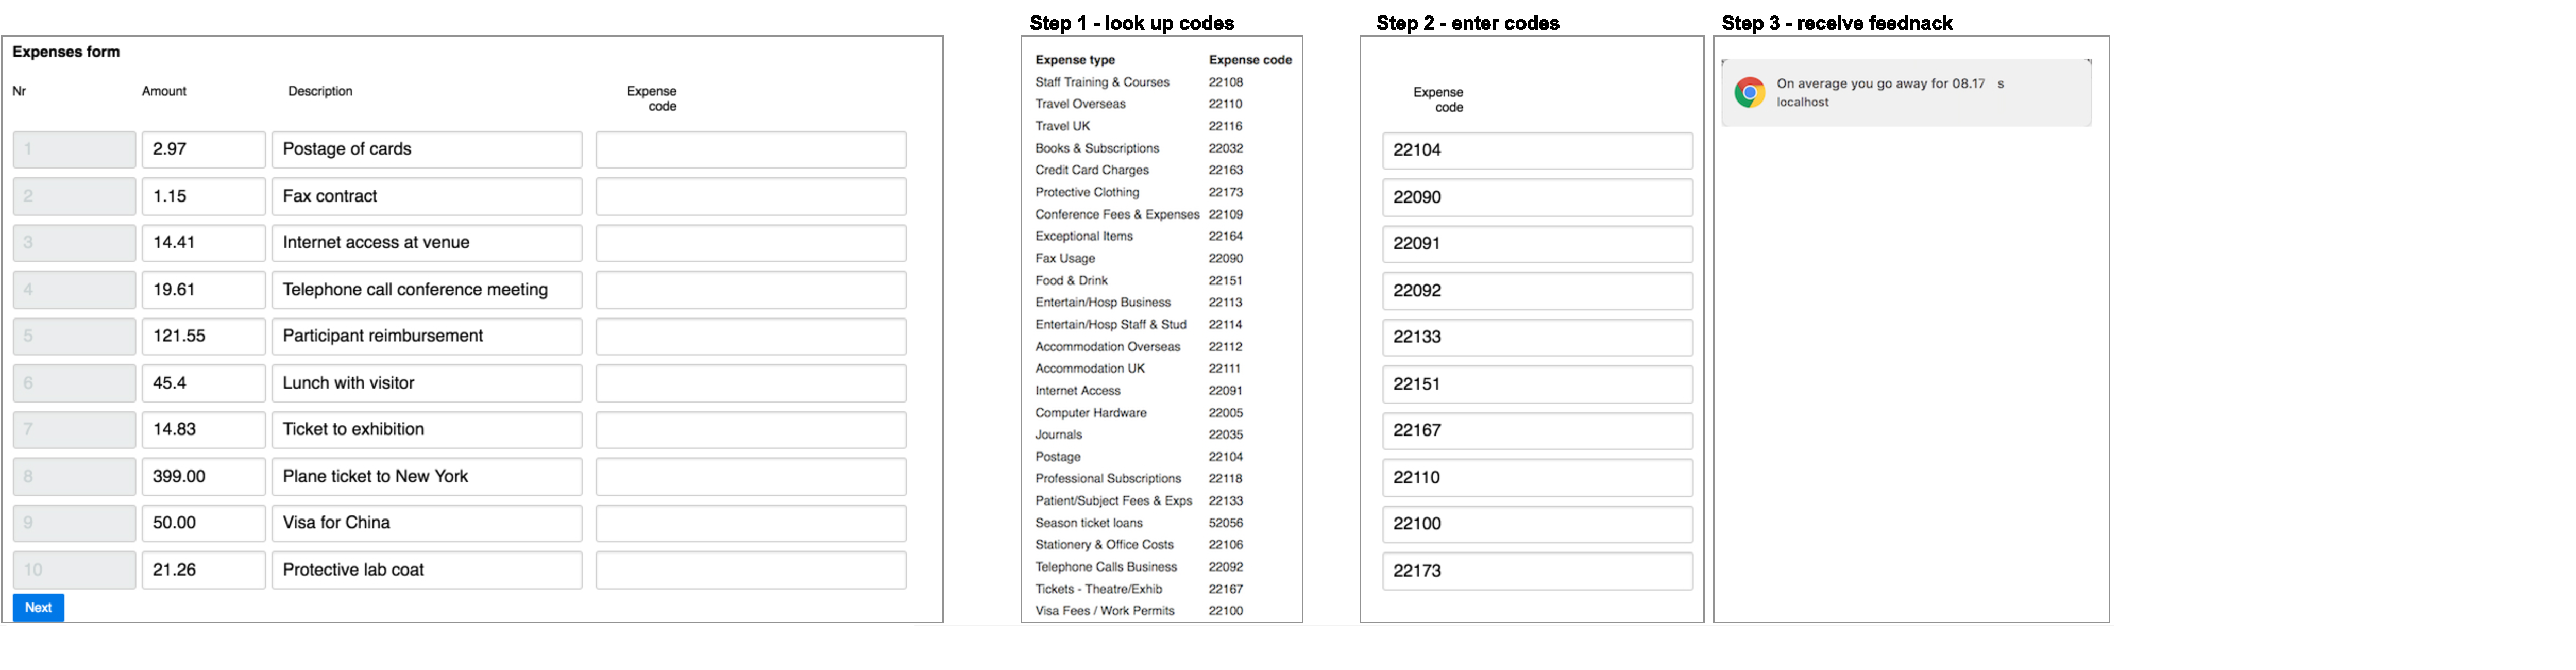
\includegraphics[width=\textwidth]{images/ch56/ch56-taskinterface.pdf}
\caption{The data entry task as shown in the browser. Participants had to look up codes from their email (Step 1) and enter this into a sheet (Step 2). After every trial, the notification condition received time information (Step 3)}
%\vspace{-3pt}
\label{fig:ch56-Figure1}
\end{figure}

\subsubsection{Procedure}
The study was advertised online with a brief description and a website link to sign up. Participants signed up for the experiment by entering their email address, and were sent an email with the table of expense categories and expense codes. The email also included instructions with a new link where the study was available. Participants were asked to complete the task on a desktop or laptop computer and open the experiment in Google Chrome, Firefox or Safari. Participants were not informed beforehand which condition they had been allocated to, and were told the purpose of the study was to understand how people perform data entry tasks. Participants in the notification condition were informed that they would receive notifications during the experiment. 
Participants first read an online consent form on the website, and were not able to continue to the experiment until they had agreed to the consent form. Participants in the notification condition received an additional dialog box to enable notifications in their browser, and had to click 'OK' to continue. Participants were instructed to have both their email and data entry window open on the same device, and to keep both windows maximised at all time, to ensure they had to switch back and forth between the two windows. Participants who made no recorded switches would be excluded from the dataset. 
After completing all experimental trials, participants were shown a page of debriefing information, explaining the purpose of the study. An email address was included as a point of contact if participants had any further questions. Participants took between 10 and 20 minutes to complete the experiment.

\subsubsection{Pilot study}
A pilot study was conducted with four colleagues to test the study set-up. Initially, the notification was set-up to appear on every switch, and showed the duration of the last interruption, instead of the average interruption time. Participant 1 looked at the notification at the start of the study, but experienced that the notification interfered with information she was holding in working memory. Upon switching, she had to memorise what expense category code she had to look up in the email, and looking at the notification made her forget what she was looking for, forcing her to go back to the data entry interface to look it up again. She therefore tried to ignore the notification for the rest of the study. For the remaining three pilot studies, the notification was adapted to only appear once after every trial, and show the average interruption duration. Two participants piloted the notification condition, and one participant piloted the control condition. Participant 3 used the information from the notification to try and find the codes in the email quicker, and consulted the notification after every trial to see whether his switches were shorter than the previous trials. The expenses task was experienced by participants as a realistic task, and all participants glanced at new incoming emails during the study.

\subsection{Results}
Table \ref{tbl:ch56-Table1} summarises the results of the conditions in terms of the four dependent variables. The number of switches, length of switches and the error rate were not normally distributed, so non-parametric Mann-Whitney tests were used to analyse effects of a notification on these dependent variables. A Shapiro-Wilk test suggested that the trial completion times were normally distributed, \textit{W} = 0.97, \textit{p} = 0.22, so an independent t-test was used to analyse the effect on trial times. 

\begin{table}
\caption{Means and standard deviations of dependent variables for each condition.}
\centering
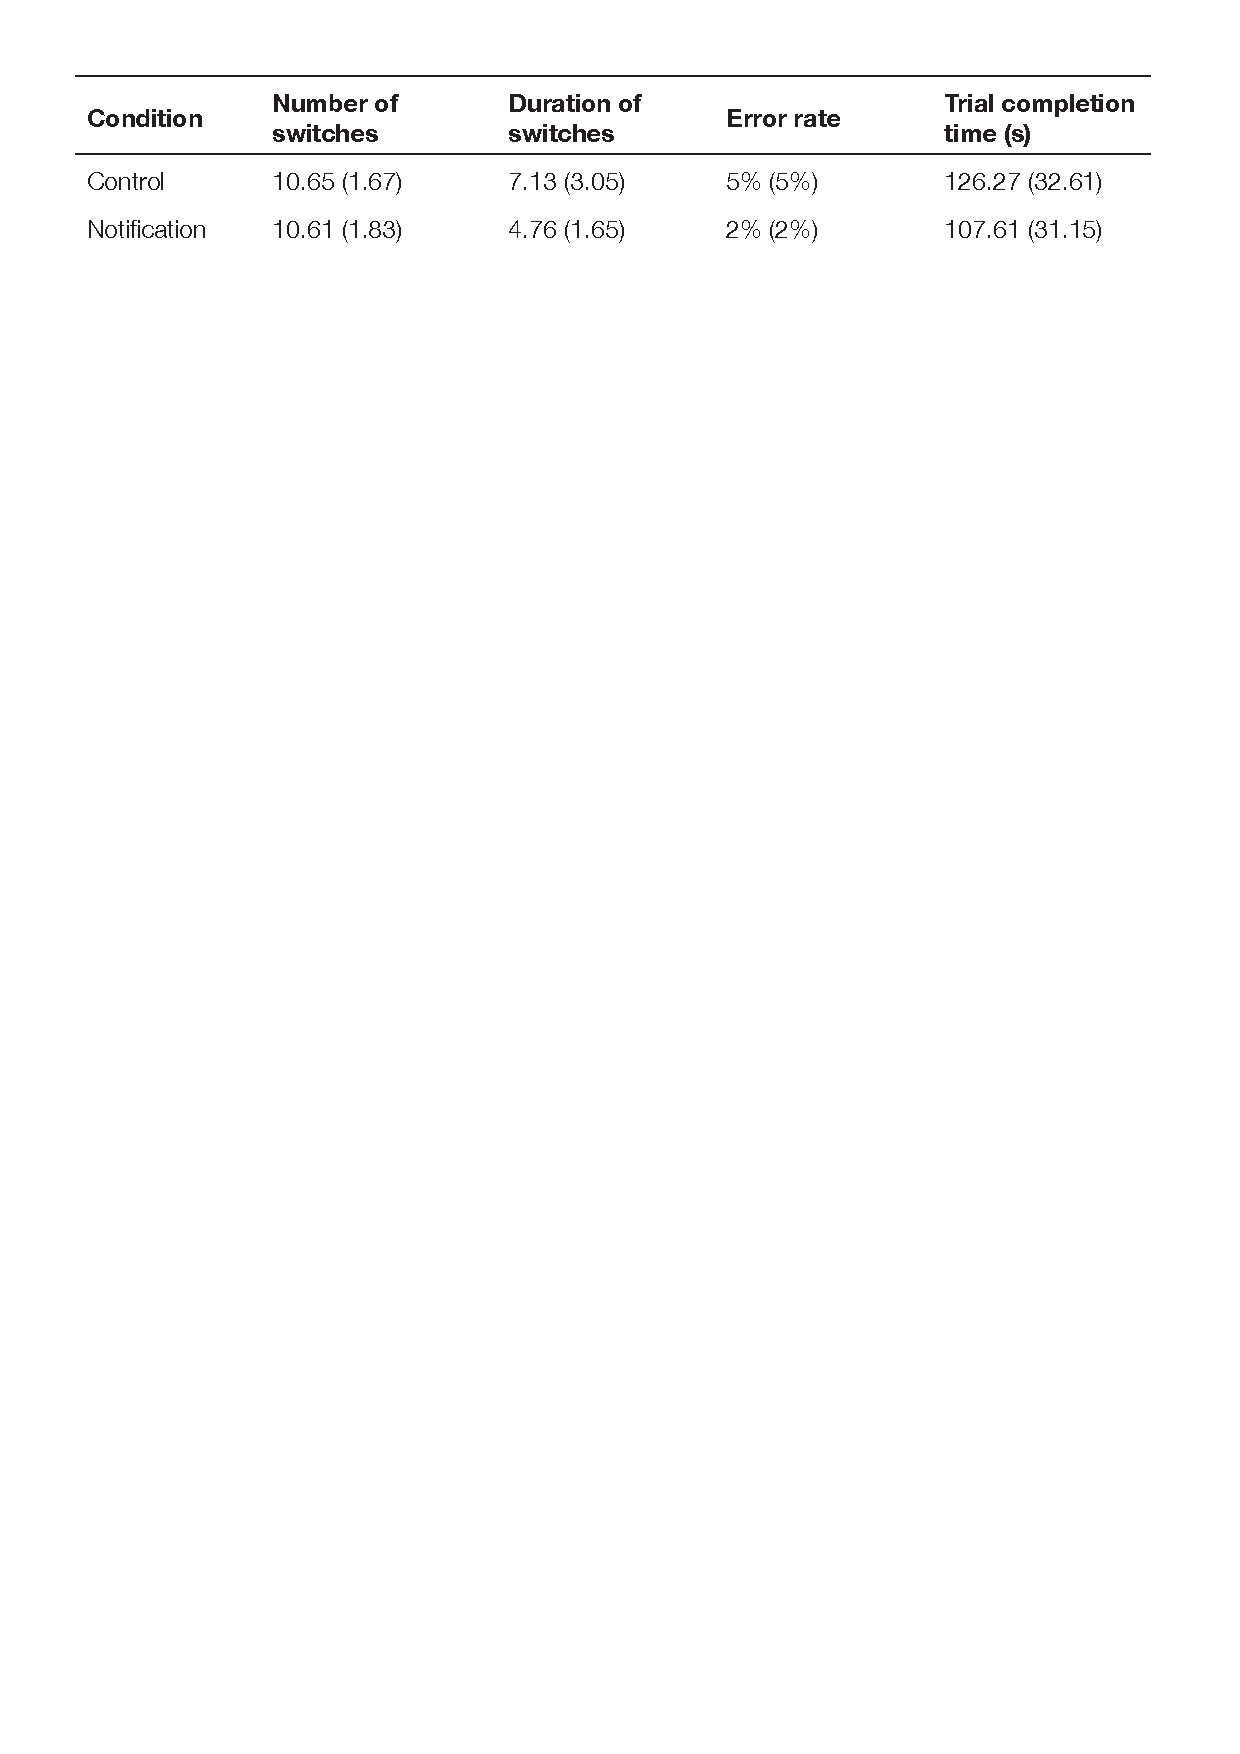
\includegraphics[width=0.9\textwidth]{images/ch56/ch56-descstats.pdf}
\vspace{-3pt}
\label{tbl:ch56-Table1}
\end{table}

\subsubsection{Cleaning the data}
In total, 87 participants signed up for the study. Thirty-four participants did not complete the task and their data was excluded from the dataset.
Furthermore, six participants made no recorded switches and were excluded from the dataset as well. Data from the remaining 47 participants was used in the data analysis.

\subsubsection{Task performance}
Participants with a notification were faster in completing trials (\textit{M} = 107.61s, \textit{SD} = 31.15s) compared to participants without a notification (\textit{M} = 126.27s, \textit{SD} = 32.61), \textit{t}(45) = 1.98, \textit{p} < .05, \textit{d} = .59.
Error rates were calculated by dividing the number of data entry errors divided by error opportunities. The error rates were significantly lower for participants with a notification (\textit{M }= 2\%, \textit{SD} = 2\%) compared to participants who had no notification (\textit{M} = 5\%, \textit{SD }= 5\%), \textit{U} = 403, \textit{p} < .01, \textit{r} = .44. 

\subsubsection{Number and duration of switches}
As can be seen in Table \ref{tbl:ch56-Table1}, the number of switches per trial was on average 10.6 in both conditions, and there was no significant difference in number of switches between conditions, \textit{U}(24,23)=243, \textit{p} = 0.6. As there were ten codes to be entered per trial, this suggests participants switched once for every piece of data entered.  
Figure 2 shows the variability in the duration of switches for the two conditions. Participants who received notifications made significantly shorter switches (\textit{M}=4.76s, \textit{SD}=1.65s) than those in the control condition (\textit{M}=7.13s, \textit{SD}=3.05), \textit{U}(24, 23) = 406, \textit{p} < 0.01, \textit{r} =.44. 
Figure \ref{fig:ch56-histswitches} shows the distribution of switching durations for the Control and Notification condition, the red line marks the mean duration. For both conditions, the distribution was positively skewed with a long tail: 97\% of the switches were under 20 seconds, but the longest switch was greater than seven minutes. To scale the distribution in one histogram, switches longer than 20 seconds are grouped as one bar. Table 2 shows the count of these long switches for each condition.

\begin{figure}
\centering
\begin{subfigure}{0.5\textwidth}
\centerline{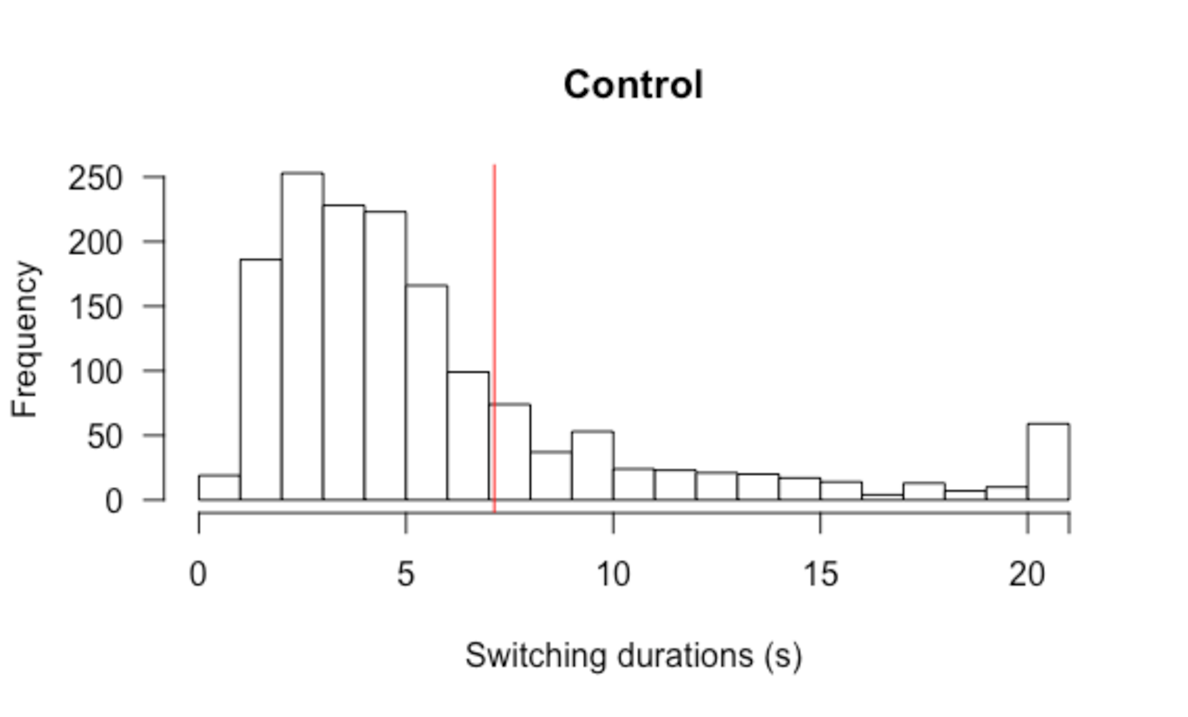
\includegraphics[scale=0.5]{images/ch56/ch56-histdurSwitches_Control.pdf}}
\end{subfigure}
\begin{subfigure}{0.5\textwidth}
\centerline{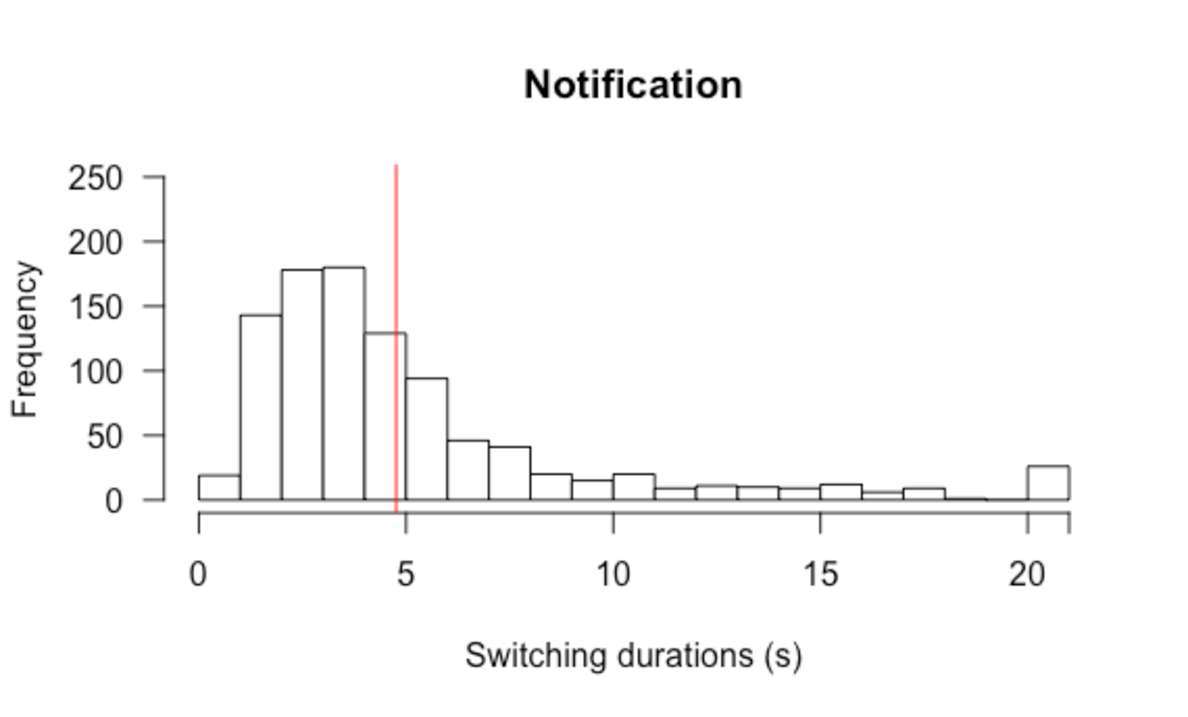
\includegraphics[scale=0.5]{images/ch56/ch56-histdurSwitches_Not.pdf}}
\end{subfigure}
%\vspace{-3pt}
\caption{Histograms showing the distribution of switching durations for the two conditions; switches longer than 20 seconds are grouped in one bar at the right side of the histograms. The red line marks the mean switching duration.}
\label{fig:ch56-histswitches}
\end{figure}

\subsubsection{Interkey intervals}
The primary measure to analyse switching behaviour were focus and blur events. These measures include any switch from the task window to another computer window. While this provides a good measure of digital switching behaviour, it cannot capture task switches outside the device because the task window remains in focus during these task switches (e.g., a user might pause to fetch a paper document or make a cup of coffee). To help capture this broader range of instances of possible task switching behaviour, we look for longer pauses in task activity captured by an analysis of inter-keystroke interval (IKI) data. Though these intervals may have also been moments where participants had briefly paused for thought, extremely long intervals between two keystrokes may point to moments where a participant switched to doing something else. The IKI data presented here excludes intervals where a window switch was recorded, as these moments have already been analysed in the previous section.

There was no significant difference in duration of IKIs between the Control (\textit{M} = 1.70, \textit{SD} = 0.91) and Notification (\textit{M} = 2.02, \textit{SD} = 1.60), \textit{U}(24, 23) = 261.5, \textit{p} = 0.9. Figure \ref{fig:ch56-histikis} shows the distribution of all IKIs for both conditions. As can be seen from these histograms, the majority of IKIs were under one second, which suggests people were typing (source of typical typing speed to support this claim?).  There were however some instances when there were long delays between keypresses: the longest measured IKI is four minutes. In the histograms, IKIs longer than five seconds are grouped in one bar. To give a closer view of longer IKIs, Table 3 shows the frequencies of long IKIs. These long IKIs were more than two deviations from the mean, and may have been additional task switches. However, we do not know for certain what people were doing during these instances, and what an appropriate IKI threshold would be to safely assume people had made a task switch. Therefore, we mainly focus our conclusions on our analysis of explicit window switches, and merely present the long IKIs to indicate that in addition to window switches, there may have been additional moments where people switched tasks. 

\begin{figure}
\centering
\begin{subfigure}{0.5\textwidth}
\centerline{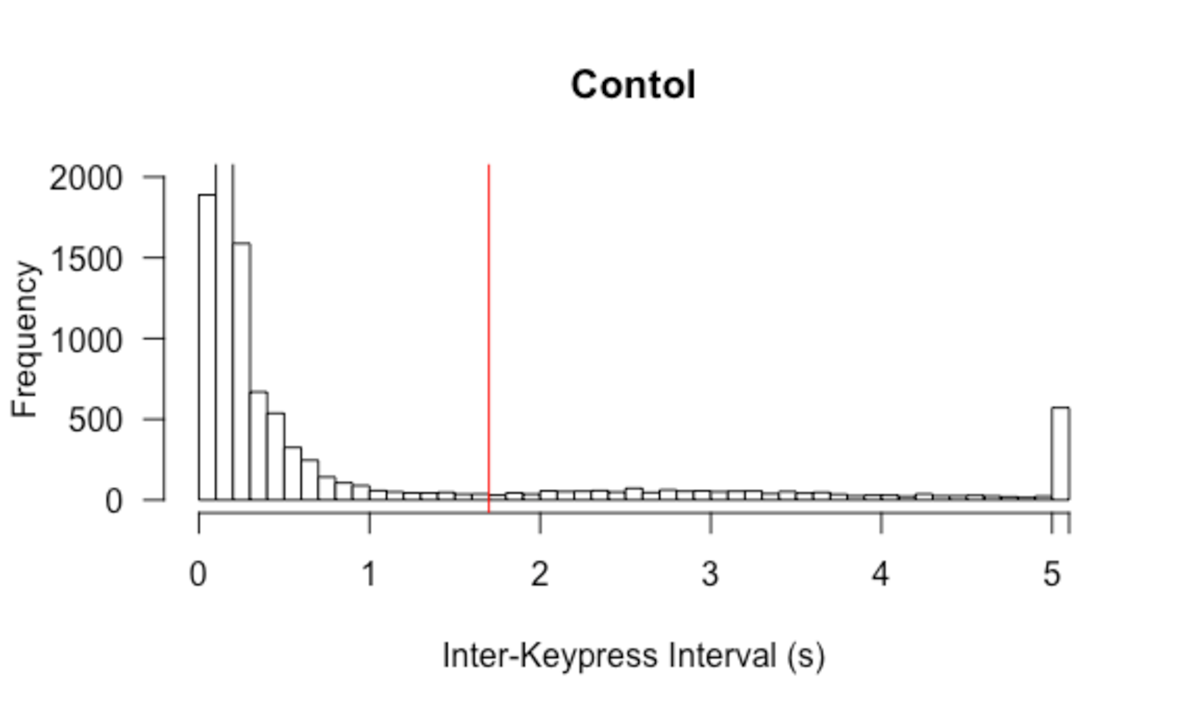
\includegraphics[scale=0.5]{images/ch56/ch56-histIKIs_Control.pdf}}
\end{subfigure}
\begin{subfigure}{0.5\textwidth}
\centerline{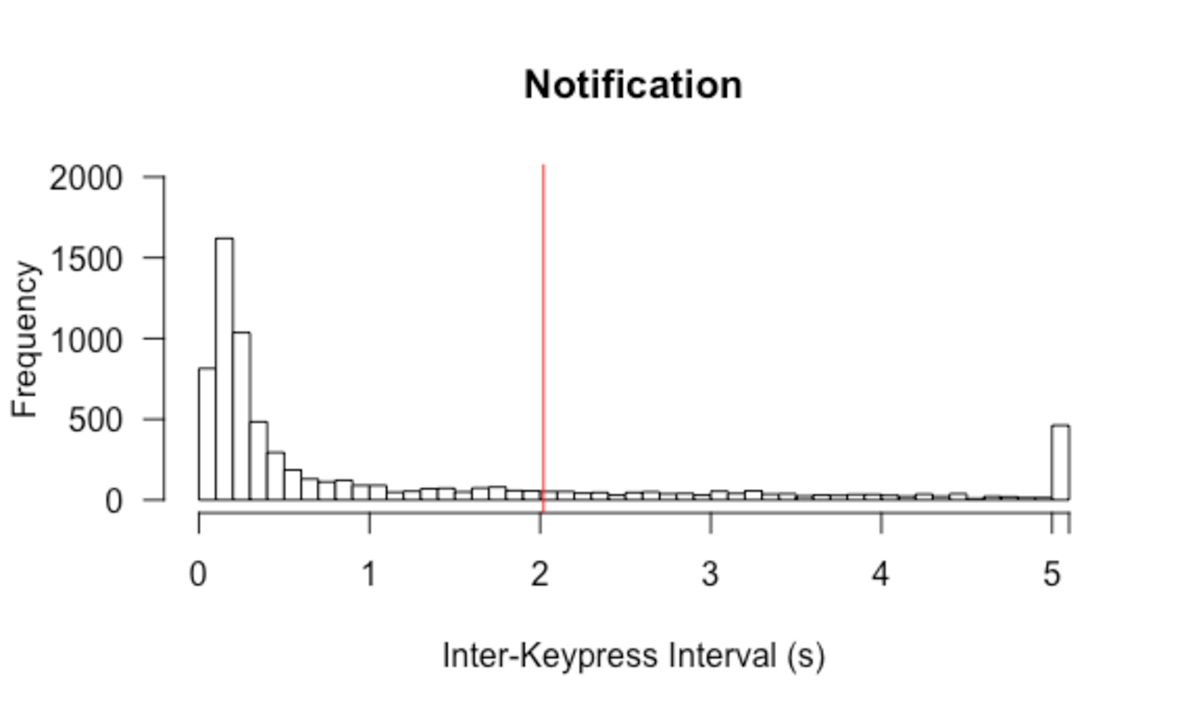
\includegraphics[scale=0.5]{images/ch56/ch56-histIKIs_Not.pdf}}
\end{subfigure}
\caption{The distribution of inter-keypress intervals for the two conditions; switches longer than five seconds are grouped in one bar at the right side of the histograms. The red line marks the mean IKI.}
\label{fig:ch56-histikis}
\end{figure}

\subsection{Discussion}
The aim of this study was to see whether showing people how long they switch on average reduces the number and length of their switches. The results show that people can benefit from receiving feedback on the length of their switches: participants made shorter switches, were faster to complete the task, and made fewer errors. These findings suggest that shorter switches can lead to better task performance, and are in line with previous studies connecting the duration of an interruption to its disruptiveness \citep{Altmann2017, Monk2008}.

Nevertheless, as even short interruptions can have a negative effect on performance \citep{Altmann2014}, it was also measured if the number of switches were reduced. Interestingly, feedback on switching duration did not reduce the number of switches as in prior work \citep{Gould2016a}. This could be explained by the moment in the task that people received feedback. In Gould et al.'s study, feedback appeared after every switch. Participants may have tried to reduce switches, either because they were more aware of every switch or because they wanted to avoid the message. In contrast to our study, their participants were not supposed to switch, so the number of switches was lower. In the current study participants were switching more often as they had to as part of the task: on average, they switched once for every data entry (i.e., ten times per trial). Giving notifications at every switch would have had the risk of overexposing participants to notifications and limiting its usefulness \citep{Cutrell2001, Whittaker2016}. Therefore, feedback was only given after every trial. Future data entry studies that require fewer switches are needed to see if a notification upon every switch can reduce both the number and length of switches. Moreover, because the notification only showed information regarding the duration of switches, participants may have focused on reducing the duration, rather than number of switches. 

The current study used focus and blur events to analyse switching behaviour. This meant that task switches outside the device, with the task window still in focus, were not captured. Possibly participants learnt to not interrupt themselves when they were away from this window, but after they had returned to the window. Without an accurate estimate of how long participants should take to complete the task, it is difficult to determine moments at which participants were away from their computer \citep{Rzeszotarski2013}.  Using other techniques, such as prompts at random intervals to confirm people are still working on the task, may be able to give a further insight whether our intervention changes overall self-interruption behaviour. 

Most studies on self-interruptions introduced an artificial distraction, such as chat messages, to measure when, how long, and how often people self-interrupt to attend to this distracting task \citep{Katidioti2013, Salvucci2010}. The current study makes a methodological contribution by using participants' own personal email inbox, based on the assumption that email provides a source of distraction \citep{Hanrahan2015, Mark2016}. However, in the current study, participants only needed to find and open an email once. Once they had this email opened, they did not have to re-find it in their inbox for the remainder of the experiment, and may have had this email maximised on their screen, hiding incoming messages. In practice however, people have to first find the email in their inbox, which can partly contribute to the distraction. Our study has already shown an effect on behaviour by switching to an email inbox. It is expected there might be a higher potential for distraction if people have to also find the correct email in their inbox.

\subsubsection{Bridge to next study}
The results of this experiment indicate that showing people how long they switch on average reduces the duration of switches and can improve people's task performance. The work makes a contribution to our understanding of switching behaviour for routine data entry tasks to distracting, but task-relevant, applications such as email. The results also suggest ways in which tendencies to attend to distractions might be mitigated, and can provide a useful pointer for the design of productivity interventions to improve focus. In the current study, an experimental task was used in order to measure task performance. 

The study did not find any effect on the number of switches. However, as the number of switches indicate, participants presumably only switched to look up information, and did not switch to other tasks, interruptions or distractions. When people are doing their own data entry work, they may not have to switch as often as in the current experiment, but on the other hand they may interrupt themselves more to attend to other tasks and interruptions. To evaluate whether the positive effect of time feedback on people's switching behaviour can extend to naturalistic tasks, Study 7 tested the notification with office workers doing their own data entry work,

\section{Study 7: Looking up information for expenses in an office setting}
\subsection{Introduction}
In order to understand whether the notification would have the same effect on a naturalistic data entry task, Study 6 was followed up with a field study testing the notification with data entry workers doing expenses work. To measure self-interruption behaviour during their work, participants were asked to install a free trial version of ManicTime \footnote{https://www.manictime.com} for two weeks. ManicTime is a time tracking software, which tracks application and web page usage. In addition, half of the participants were asked to install a browser extension, and use it when they are processing expenses. Every time participants switched away from the browser window in which they did their expenses work, the extension showed a notification similar to the notification used in Study 6. The purpose of the study was to see whether a notification had an effect on self-interruption behaviour. To get a quantitative measure of self-interruption behaviour, ManicTime data was used to derive number and duration of window switches during expenses work. In addition, participants were interviewed to explore whether and how the use of both the extension and ManicTime led to any conscious changes in their behaviour.
 
The study aimed to address the following research question: how does feedback on interruption length have an effect on people's self-interruption behaviour during expenses work in a finance office setting? 

\subsection{Method}
%DESIGN
To study the effect of a notification on people's self-interruption behaviour, a between-groups design was used and participants were divided into a control group and experimental group. The control group was asked to install ManicTime for two weeks. They were told the purpose of the study was to understand how people in offices manage tasks, windows and applications. The experimental group additionally were asked in the second week to install Focus. They were told that this extension would give additional information on the current task they were working on. Other than this distinction, all instructions were identical between the two groups. 

Four participants were unable to use Google Chrome, and therefore the extension, for their work. Therefore, these participants were part of the control group. To make the groups even, one other participant was randomly chosen to be allocated to the control group; the remaining participants were allocated to the experimental group. 

%If the main task page is not in focus, either because participants have switched to another page or if it has been inactive for x seconds, they will receive a notification with a warning message. Upon returning to the expenses page, they will receive a notification indicating how long they were away from the page. The control group will be asked to install the plug-in, but will receive no notifications. It is explained that the purpose of the study is to log people's switching behaviour, and participants will be able to see their data at the end of the study. Participants will be asked to use the add-in for one week in which they have to do a substantial amount of expenses work, and keep a diary of their experiences. Within a week of finishing the diary, a follow-up interview will be scheduled to gather more detailed explanations of participants' experiences of using the add-in.

\subsubsection{Participants}
Nine participants (six female) took part in the study. They were office workers at finance administration offices at a public university, and were invited to participate via emails sent to departmental mailing lists and snowballing. Participants worked in an open plan office, and seven participants occasionally worked from home. Participants’ work included administrative and supportive tasks, such as processing payments, expenses, managing budgets, and responding to queries by university staff and students. The majority of participants’ work was carried out in a web browser, and revolved around a number of web-based data entry systems. None of the participants had used a time or task management tool before. Participants were reimbursed with a  \pounds 20 Amazon voucher after completing the study. 

%Ten participants (three male) took part in the study. They were recruited using the same recruitment methods as Study 1 and 2. Invitations were sent to opt-in mailing lists of Finance departments of a university, and forwarded by contact persons and people who had already participated. None of the participants had taken part before in any of the studies reported in this thesis, but were drawn from the same population. None of the participants had used a time management application such as ManicTime before. Participants were reimbursed with a \pounds 20 Amazon voucher.

\subsubsection{Materials}
The notification was implemented as a Google Chrome extension using HTML, JavaScript and CSS. After installing the extension, an icon was permanently visible in participants’ browser (see Figure 7). To use the extension, participants had to navigate to a web page in their web browser that they wanted to focus on, and click on the icon of the extension. Upon clicking on the icon, a pop-up appeared saying that the current web page was now the main task page, which indicated the start of a task session. Every time participants switched away during the session from this web page to another computer window, such as a different browser window, a document or an application, they received a notification indicating how long on average they go away for when switching away from the main task page. If participants switched away from a page for the first time, the notification showed a message that no switching data was available yet. To calculate the average switching duration, the extension recorded and saved the number and duration of switches away from the main task page for the whole session. Participants ended a session by closing the page. Due to security restrictions of browser extensions, the extension was unable to save any session data after a session had ended. 

The presentation of the notification was similar to Study 6 but differed in one important aspect. Whereas the notification in Study 6 appeared once after every trial, in this study it appeared upon every switch away from the task. Based on the observations and interviews reported in Chapter 3, I anticipated participants switched less frequently for their main work compared with the experimental task, and therefore a notification at every switch was not considered to be too disruptive.

To get an understanding of people’s interruption and window switching behaviour, participants were also asked to install ManicTime, a computer logging software which records and stores the time spent in all application windows. We initially intended to give the extension to only half of the participants to see if there was a notable difference in interruption behaviour between people who used the extension compared to people who did not. However, five participants were unable to install ManicTime on their work computer, and could only use the extension. Due to this lack of quantitative data to make a fair comparison, we therefore distributed the extension to all participants and mainly focused on the interviews and people’s experience of using the tool. A summary of ManicTime data of the remaining four participants (P3, P4, P5 and P9) is included in this chapter and used to complement the qualitative interview data and give an insight in the fragmented nature of people’s work.

\subsubsection{Procedure}
Participants who expressed interest were sent an information sheet and consent form to read and sign. They were sent an overview of the study, instructions to install the tools, and a post-study interview was scheduled.
The study was divided into three stages:

\paragraph{Week 1: Install ManicTime}
In the first week, participants were sent instructions to install ManicTime on their work computer. They were given the option to pause or stop the application from running at any time. They were told that they were free to choose if, when and how often to look at the information, but that it was important to complete at least one expenses task with the application running. 

\paragraph{Week 2: Install the browser extension}
In the second week, participants in the experimental condition were asked to install the extension. Again, they were instructed that they were free to choose when and how often to use the extension, but that they had to use it for at least one expenses task. Even though the second week was the same for participants in the control condition, they were also asked to complete at least one expenses task in the first week, and another expenses task in the second week. This instruction was included to compare if any observed changes in switching behaviour were due to the browser extension, or if participants simply became more aware of their switching behaviour in the second week.

\paragraph{Week 3: Interview}
%Participants were sent an email with instructions on how to share their database and remove the tools from their computer.
In the third week, participants were interviewed about how they currently manage documents, applications and tasks for their work, and asked questions on their experience of using the tools. In particular, it was discussed whether and how they used or would use the information that the tools provided, and whether they made any changes on how they went about their work. They were asked to share their ManicTime database for further analysis. Participants were offered guidance and assistance on deleting or adapting any data in their database, such as removing application and website names. Participants were still eligible to participate, if they did not wish to share their database.

After two weeks of using the tool, participants were interviewed at either the participant’s or the interviewer’s office. The semi-structured interviews were structured around the following themes: how participants currently manage interruptions, tasks, time and information, the context of using the extension, the usefulness of the information provided by the extension and ManicTime, and whether they made any changes on how they managed their work. Participants who did not install ManicTime were presented with screenshots during the interview, and discussed the usefulness of this type of information compared to the time information of the extension. Participants were asked to share their ManicTime data for further analysis. They were offered guidance and assistance on deleting or adapting any sensitive or confidential information in their data, such as application and website names. An interview lasted about 60 minutes and was audio recorded. 

\subsubsection{Pilot study}
A pilot study was conducted with two participants. One participant was a colleague and was sent instructions to install Focus on his computer. The purpose of this pilot session was to see whether the installation instructions were clear and to test the extension on other people's computers. The participant had the tendency to hover over the notification to stop it from disappearing, which placed extra buttons over the end of the notification message. Therefore, the message was shortened and the most important information, namely the duration of switches, was placed at the front of the message to ensure it was still visible upon hovering.

A second pilot session was then conducted with an administrator working at the same university as the study participants, who was asked to install ManicTime and Focus on her work computer. The purpose of this session was to ensure the tools could be installed on the work computers of the university, and that the extension worked with the university finance system.

%Findings pilot study

\subsubsection{Ethical considerations}
Participants were informed before undertaking the study that they would be asked to share their ManicTime database at the end of the study. However, a disclaimer was added in the invitation and instruction emails that participants were still able to take part, if they did not wish to share their database. It was made clear what data ManicTime recorded, and that Focus did not store any data. They were given instructions on how to pause the application from running and how to delete certain parts of the data, and were offered assistance to help further change the database into a state they were comfortable sharing. 

\subsubsection{Data analysis}
Though ManicTime was piloted on a work computer of the university before starting the study, three participants were unable to install ManicTime on their work computer due to firewall restrictions. Furthermore, two participants opted out of using Focus as they used a browser different from Google Chrome for at least parts of their work. Therefore, ManicTime data of the remaining four participants was used to complement qualitative explanations of their task switching behaviour, but it was not analysed quantitatively as previously planned to compare switching behaviour with and without the extension. Instead, the primary focus of data analysis was on the post-study interviews and participants' subjective experience of using the tools. The interviews were transcribed verbatim, and analysed using thematic analysis.
\subsection{Findings}
%Reflective and current information
Interviews were transcribed verbatim, and a thematic analysis was used to analyse the interviews. Participants gained some insights to change their behaviour based on the information they received from the extension. People’s switching behaviour as shown by the ManicTime data is reported first. I then discuss the usefulness of time feedback to manage interruptions around the following themes: awareness and change of behaviour, the type of interruptions, the effort to record and use data, setting goals, and the work environment.

\subsubsection{Switching behaviour}
Participants’ working hours differed slightly, but all participants worked at least ten hours per day during the study. To make the data comparable between participants, we only considered data between 9am and 7pm, during which all participants were at work. 

Table 4 summarises the average number and duration of focus on a computer window screen. The mean duration of focus is about 34 seconds, with the longest focus being 48 minutes (2893 seconds). On average, participants made 830 computer window switches per working day. The distribution of window focus durations was positively skewed with a long tail: 95\% of the distribution is plotted in Figure 8, illustrating that participants were rarely focused on a window for more than a minute. Together with the interview findings, the data shows that participants’ work was characterised by short durations of focus and frequent window switches. Figure 9 and Figure 10 show the average number of daily window switches and focus durations over the ten days of the study.
In addition to computer window switches, participants also made a smaller number of non-digital interruptions, for example when taking a break or attending a meeting (see Table 4). On average participants made three daily non-digital interruptions which lasted about 29 minutes (1741 seconds). 

\subsubsection{Awareness and changing behaviour}
Participants were largely aware they interrupted their work frequently and considered it the nature of their job: they regularly had to stop their work to look up task-related information, and had to address ad-hoc queries and requests from their department. Some interruptions were hard to avoid because they were urgent, important, or necessary to progress with work. The extension however made participants realise they were unaware these interruptions were much longer than they considered necessary. The notification was a trigger to then reflect on the reasons for this:

\textit{“It's a shock, because I knew it was bad, I didn't think it was that bad. (…) So it's reflecting on, actually, a two-minute task is turning into a 15-20 minute task - why is that? (…) Why? But again, it's distractions.”} (P9)

If they realised upon reflection that they were distracted by irrelevant activities during these interruptions, participants tried to avoid these activities and focus on the goal of the interruption, for example by setting an explicit time limit for themselves:
 
 \textit{“It would give me a chance to maybe cut out some stuff that I felt wasn’t really relevant. (…) I spent an hour yesterday on Google, what was I doing? It’s like surfing the net, but it’s not, because you’re looking for something in particular. (…) OK, I’m going to make sure that I only spend twenty minutes on Google.”} (P6)
 
Some interruptions were not urgent, but participants were used to addressing them anyway if they were presumed to be ‘quick and easy’, so they did not have to remind themselves to attend to it later. The notification however made participants reflect on the occurrence and actual length of these interruptions, and whether they always needed to address each interruption immediately:

\textit{ “It made me realise how long I was spending, spending/wasting, doing other stuff. I think it affected me in the sense that I wanted to take fewer breaks. Well, by breaks I mean, it’s just going to do something and then ending up chatting with someone.”} (P3)

\textit{“I need to work on time management and (…) not spending my whole day answering irrelevant queries.”} (P9)

\subsubsection{Effectiveness of time feedback for different types of interruption}
Participants found the feedback especially useful when they switched to sources they knew were distracting, for example search engines, instant messaging tools, and email. Participants needed to access these sources for work, so it was difficult to avoid them:

\textit{“As everyone says, ‘we’ll just switch email off’ (…). But you can bet your life that there will come a moment in whatever task you’re doing you think: Oh! I have to open up email. And the moment you open up your email, that’s it.”} (P2)

Two participants (P3, P7) found the extension mostly useful if they were about to interrupt themselves for non-work related activities, as the notification helped as a reminder to either stay focused on the task, or to not spend too long on the interruption. If they however had to be in a different computer window for a while as part of the task, the information was not considered useful:

\textit{“I think it'd be really, really useful, but not for necessary work tasks. (…) I’ve been spending 15 minutes on Moodle, and my main page is X or Y. I don’t care to go to that main page or not. So whether you could setup different ‘main’ pages… but then that would be complicated.”} (P3)

P7 was the only participant who, upon viewing the time information, was not surprised by the time she spent on work-related interruptions. She considered the amount of time necessary to complete her work and did not see any room to improve on this: 

\textit{“To me, it doesn't kind of make me think: 'Oeh, I've been away too long'. I just think: OK, well I'm roughly aware that I've been away for an hour (…), I don't see how it kind of links with being more productive. Unless I suppose, you're really easily distracted.“} (P7)

Participants also dealt with interruptions taking place outside of the computer: for example, participants were interrupted by their colleagues or phone calls, or interrupted themselves to print something off. As with digital interruptions, there was again no clear distinction between distracting and work-necessary sources, so participants could not always manage distracting self-interruptions by avoiding these during work:

\textit{“My phone is a distraction for me. (…) I put my phone in a tray under a load of documents. But then I’m in Whatsapp work groups. So I converse a lot with a professor via text.”} (P9)

Because the extension only provided time information about digital interruptions, some participants felt it provided an incomplete picture of their interruption behaviour. This is illustrated by the following quote from P2 who, upon making the first digital interruption away from a task, read in the extension that there was no interruption data available yet: 

\textit{“That's when I sort of thought: 'Oh, that's not really saying much, is it?' Because it's not actually true. Because of course there were interruptions.”} (P2)

ManicTime provided participants with information on their non-digital interruptions, and participants considered this a good complement to the information that the extension provided. If the PC was inactive, and participants came back from inactivity, ManicTime presented users with a window on the screen saying how long they had been away for (see Figure 11), and gave participants the option to write down what they had been doing while they were away.

\subsubsection{Effort to view and use time data}
Participants appreciated that the extension presented them with information during a task, as they would forget to look at it otherwise:

\textit{“It needs to be shown to you, to make an impact.”} (P6)

One participant (P4) said she sometimes forgot to start and use the extension during busy periods at work. Another participant (P3) found ManicTime less intrusive than the extension, because it runs in the background, but also said he often failed to remember to open and look at ManicTime data, as he was busy with work. In contrast, the notification worked as a trigger for participants to reflect on their behaviour.

Participants reported that the concise and precise measure of the average interruption time was easy to read and interpret during a task. It was also clear what action to take, and participants read the information to decide whether they should reflect on past interruptions. To aid their reflection, some participants wanted to get insight in additional data of what they were doing during these interruptions. P9 combined the extension with ManicTime to contextualise the interruption:

\textit{“[The extension] popped up and it said: ”You go away for 7 minutes and 33 seconds. I would then have a browse [in ManicTime] And then I think: oh my gosh, I've been on emails for an hour! I haven't got anything done. So yeah, I checked it quite a lot. More so because I was so shocked. And so, I'm so interested to know, actually, what I'm doing at work.”} (P9)

Two participants, who did not have ManicTime installed, wanted to use the extension to see more information. For example, they wanted to see a log of all of their past interruptions, and explore a pattern of their behaviour:

\textit{“It [the notification] kept on coming up, (…) and you can't click on it, because it's not taking you anywhere! But yeah, I found that a shame. Because I could see the benefit of it, and it would have been really, REALLY interesting.”} (P2)

\textit{“I would like to see, just on a weekly basis, exactly what I’m doing, (…)  what was productive and non-productive time.”} (P6)

However, participants who used ManicTime and did have access to past behaviour, primarily opened it after being triggered by the notification to see what they had been doing at a specific moment, and rarely used the application to look at patterns of their overall activity or aggregated data. They briefly looked at the rest of the data out of curiosity at the start of the study, but the extensiveness of the ManicTime data made it unclear to participants what action to take from the data. It was considered too effortful and time-consuming to find this out themselves:

\textit{“I didn’t go into too much detail with it. One of the reasons is that, it would take me a lot of time and effort to use this information, to help me work better or quicker, or more efficiently. And this is either something that I don’t have time to do, or I can’t be bothered, depending on the day.”} (P3)

\textit{“I just can't see myself spending the time using something to help me spend time on things! [laughs] I just have quite a lot of things to do, that I’d rather not spend more time organising that, I’d rather just get it done.”} (P5)

Potentially giving participants a log of a specific aspect of their behaviour, in this case the occurrence and duration of interruptions during a specific task, will be more valuable than all of their activity, as it can save participants time of filtering and interpreting the data, and help them look at the impact of changing a specific habit over time. 

\subsubsection{Effectiveness of time feedback to set goals}
A clear interest among participants was to not only see how much time they spent on interruptions during a task, but also how much time they spent on a task overall. In the same way that they used time information to reflect on whether interruptions were as long as they thought they were, they wanted to reflect on whether tasks took as long as expected. Furthermore, they would use this information to be more realistic when planning tasks over time: 

\textit{“So down the line, I’d think it would be extremely useful to know how much time I’m actually spending. Because it would help me be more productive, or be more realistic in the amount of time I need for these things to happen.”} (P3)

\textit{“I'm quite keen to know how much time I'm spending and doing which task. [In addition to] how much we're away from the task.”} (P8) 

Currently, participants planned tasks they wanted to complete on either a daily or weekly basis, and implicitly took the time each task would take into consideration. However, given the fragmented nature of their role and the frequency of interruptions, it was difficult to estimate how long they actually spent on these tasks: 
\textit{“They’re very loose goals, (…) I think that might take me 3 hours, and I’d want to get that done in one day. But yeah, obviously, things quite often take longer than I think I will, because then when I’m doing them, I might get interrupted.”} (P5)

\textit{“I think time is quite important to monitor, sometimes it goes really fast, sometimes it doesn’t, but this thing is actually telling you exactly what has been happening. (…) Now I have no, I have just a rough measure, which is how I feel, rather than a precise measurement.”} (P3)

The interest to see time on tasks was related to the theme that participants wanted to complete as many tasks as possible within a certain time frame, and were driven in their work by tasks and deadlines. Completing tasks made them feel a sense of achievement, and this was also one of the reasons why they addressed an interrupting task immediately, if they thought they could complete it quickly:

\textit{“I love that feeling! It is a great, wonderful feeling, psychologically, you think: that’s DONE!”} (P2)

\textit{“It kind of contradicts what I told you before about (…) how I jump on them [incoming tasks] and finish them. But at the same time, it’s because I don’t want to have three things at once going. I want to finish, finish, finish.”} (P3)

\textit{“I strive on achieving, and if I’ve not ticked something off my to-do list, I don’t feel like I’ve achieved anything that day. (…) That’s where ManicTime has really helped me, (…) actually look at the log, (…) I do feel like I am achieving, even though on paper, I’ve not ticked anything off.”} (P9)

Two participants also wished to set time limits on their interruptions, and wanted to get reminders during the interruption to return to a task. As some applications were used for both work and non-work activities, it would be difficult for a time application to automatically detect an appropriate time limit:

\textit{“Say you have to work on that specific document, and then you end up spending half an hour on Slack, chatting to your colleagues, it would be good if something's like: mate, work. Stop doing other things. But it’s really hard to know what people are actually doing on these things.”} (P3)

\textit{“If you’re going on Word, and you’re typing a letter or you’re just making random notes. You’re still on Word, but the letter’s obviously more important than just making random notes. (…) Maybe the next stage would be that you set it up where you’re only allowed 30 minutes, and an alarm sound [will go off] to say your 30 minutes are up. So you know what you’re doing, and sort of regulating it, to fit in with what you want to achieve.”} (P6)

\subsubsection{Different work environments}
Seven participants worked from home on occasion, and though participants only used the extension in the office, their descriptions of their office and home environments indicate that participants may in particular benefit from time information during afternoon work in the office, when participants were more prone to interrupt themselves and get distracted. In general, the office was seen as a more distracting environment and participants saved up tasks that required focused attention to complete at home. They received fewer external interruptions:

\textit{“You’re working from home for a specific purpose, and therefore you don’t really want to be disturbed. Unless it’s absolutely urgent.”} (P2)
 
\textit{“I get fewer emails, definitely. (…) If I’m not there, 7 out of 10 enquiries, they deal with themselves.”} (P9)

At home, participants also reacted to interruptions differently:

\textit{“From home it’s a bit different, I normally look at the emails but I generally try not to respond, unless it’s too urgent. But at work, when I’m here, (…) if it is not too urgent, but still I can find that is nice and straightforward, I just straight reply back. But at home it’s more focused, definitely.”} (P8)

The office environment not only exposed participants to more external interruptions, but all seven participants reported there were also more sources to get distracted. For example, most participants had multiple computer screens and kept the majority of documents, browse windows and applications open on their work computer, even after they had finished with them. These windows were a further source of distraction if participants were trying to find task-related information in one of the windows:

\textit{“It’s like 15 tabs, and I need to go somewhere. And I end up clicking all of them. And if there is one that is personal stuff, I end up reading it. And then five minutes after, I’m like: what was I doing? (…) So it’s distracting in the way that it makes me not solely focused on one thing.”} (P3)

In contrast, at home participants worked with one screen and had their main task window maximised. Another participant reported she was also less prone to react to other self-interruptions at home:

\textit{“When I’m at home, I generally don’t look at my phone for some weird reason. (…) When I’m in the office I find that I’m easily distracted, and I don’t get things done.”} (P9)

Though all participants felt that the office environment introduced more distractions during work-related interruptions, two participants expressed that there were still other, personal, interruptions at home:

\textit{“There are fewer, but there are still interruptions, but they are of a different kind. I guess in a way some of them are kind of internal interruptions.”} (P5)

\textit{“Coming to my office makes sense, if you want to work. Staying at home makes sense if you want to chill.”} (P3)

\subsection{Discussion}
The aim of this paper was to investigate whether showing people how long they go away from a task can reduce the number and duration of interruptions and improve task performance. The results suggest that feedback on the length of an interruption during the task can help people adapt their interruption behaviour in the moment and become more focused on completing a task. Whereas Study 6 showed that it reduced the duration of interruptions and made people more accurate and faster in completing a data entry task, Study 7 showed that it made people reflect on what they were doing during an interruption, and as a result they tried to cut down the length of interruptions and reduce the number of unnecessary interruptions.

\subsubsection{Implications For Design}

Previous work has highlighted several problems with existing commercial time tracking and management applications: these often are time-consuming to use, they can restrict user activities too much, and it is not immediately clear to users what action to take based on the data \citep{Collins2014, Whittaker2016}. The findings partly corroborate these issues, and demonstrate several pointers that can inform the design of time applications. 
First, when providing users with a data log of their computer activities, they need to have a specific starting point of what it is they want to find out for them to be able to use it and act on it. Participants were not interested in their overall computer activity, but were mostly interested in the time they spent on, or away from, a specific task. By presenting a simple and precise measure, in our case the length of an interruption, participants were provided with a specific target of what to reflect on and change, and did not need to go through the effort of having to interpret information of all their activity. As some participants did want to have access to more detailed information about their activity during a specific interruption, a simple presentation in the moment can be complemented by a more complete log running in the background. It would also be interesting to give users control over what information they are interested in to see in the notification. For example, most participants were not only interested in the length of interruptions during a task, but also on the length of their task overall. 

Second, by showing information during the task, participants can react and change their behaviour immediately and do not have to remind themselves to look at information later. Participants were prompted by the notification to reflect on what they were doing during an interruption, but often forgot to look back at their computer activities on other occasions.

Another promising area to investigate would be to record the interruptions and give participants insight in how their changes have an effect over time. Although it was clear to participants in Study 2 what action they had to take based on the data presented by the extension, some felt they did not have sufficient information as to whether their changes had any effect over time.

\subsubsection{Limitations}
While the results are promising, the study also has a number of limitations. Due to the limited logging data, I am unable to make any concluding claims as to whether time feedback had any significant effect on participants’ window switching and task focus behaviour over time. In addition, though participants indicated they modified their behaviour after using the extension, it is not certain whether they based their behaviour on the specific information provided by the extension, or whether the notification simply made them reflect and become more aware of their time. 

\section{Summary}
This work contributes to our understanding of switching behaviour for routine data entry work to distracting but task-relevant applications such as email. The results suggest that a simple presentation of time information during a task can mitigate distractions but still keep users in control over their interruptions, and can inform the design of productivity interventions to improve focus.  %Studies 6 and 7
\chapter{General Discussion}\label{ch:Discussion}

\begin{mynote}
\subsubsection{Chapter outline}
This chapter summarises the research findings of this thesis. It discusses the contribution that the findings make to knowledge, the practical implications, discusses limitations and suggestions for future work.
\end{mynote}

The aim of this thesis is to understand how people can better manage the time spent on inquiries needed for a data entry task, with the goal to reduce the disruptiveness of inquiries for the task. The results show that time costs can be used to encourage users to keep inquiries short, reduce the number of inquiries, and postpone them until a more convenient moment in the task. In this chapter, I first summarise the findings of each study. I then discuss the contribution of this thesis and the practical implications for tools aimed to help workers manage their interruptions in the workplace. Lastly, I discuss any limitations, outstanding questions, and how these could be addressed in future work. 

\section{Summary of findings}
Chapter \ref{ch:12} aimed to answer the first research question:

\begin{enumerate}
\item
How do people manage inquiries for data entry in an office setting?
\end{enumerate}

Using an interview study and contextual inquiry, I demonstrated that people manage physical inquiries by postponing them until a convenient moment in the task if they are expected to take time. Digital inquiries are managed by addressing them immediately as these are presumed to be quick to deal with.
%reported an interview study and a contextual inquiry study looking at the context in which office workers in finance offices conduct data entry work, and how they self-interrupt to look up task-related information during this work. 
The studies made three contributions. First, there had previously not been many studies that tried to understand data entry behaviour in the uncontrolled setting of an office workplace. Interview findings from Study \hyperref[st:Study1]{1} revealed that a critical component of this type of work is not just entering the data, but collecting this information from various sources distributed in the physical and digital work environment. Second, the study showed that inquiries were handled differently than task-irrelevant interruptions: people try to avoid task-irrelevant interruptions, but have to make inquiries as part of data entry tasks. Third, observations in Study \hyperref[st:Study2]{2} revealed that there was a difference in how physical and digital information is collected. Participants were aware that physical sources take time to access and participants therefore prepared it beforehand, or postponed retrieving it until a more convenient moment in the task. However, computer window switches during the task were commonly observed as workers often realised during the task that they needed additional information, and they presumed these switches to be quick. These switches often took longer than intended, and participants were observed being logged out of the entry system, resuming the wrong data entry task, and reported it took time to resume their work after these longer switches. The hypothesis was made that the expected time it takes to collect information played an important part in how people address self-interruptions, and that workers were unaware of the time they actually spend on digital interruptions. Though these qualitative studies gave a better understanding of how data entry work is situated in an office setting and people's self-interruption strategies during this work, the extent to which these strategies were influenced by time costs is unclear. Therefore, a series of lab experiments was carried out to study the effect of time costs on people's switching behaviour in a controlled setting.

Chapter \ref{ch:34} reported three controlled experiments aimed to answer the second research question:

\begin{enumerate}
\setcounter{enumi}{1}
\item
Do time costs affect the number, duration and timing of inquiries? 
\end{enumerate}

Study 3 showed that participants reduce the number of these inquiries, and increase the duration of them. Study 4 and 5 demonstrated how time costs affect the timing of inquiries: high time cost inquiries are postponed until later in the task, and inquiries with a low time cost are addressed first.
%to test the hypothesis that people prioritise collecting information according to time costs: they first switch to information with low time costs, and postpone collecting information with higher time costs. 
These studies showed that, in a controlled setting where participants can learn the time costs involved in accessing information, they first switch to information sources that are fast to access, and switch more frequently to these sources. On the other hand, people either prepare or postpone looking up information which takes time. Study \hyperref[st:Study3]{3} showed that if people retrieve all data from the same source, they will reduce switches between entering and looking up data if the access costs to this source increases. As it took more time to access, offloading behaviour was observed as well, and several participants prepared items they were going to need nearby, but did not use them yet. Study \hyperref[st:Study4]{4} further demonstrates that when people have to retrieve data from multiple sources, they collect and group items that are quick to access first, and leave items that take longer to access until the end. Study \hyperref[st:Study5]{5} demonstrated the robustness of the effect of time costs in a multi-task setup: when dealing with two data entry tasks, people still entered items with a low time cost first, and interleaved between tasks to enter items with low costs first. As a result, participants made more omission errors and submitted tasks before they had completed entering all the items. These studies contribute to our understanding of the effect of time costs on self-interruption behaviour to collect information: if people know the expected time duration of an interruption, they make fewer interruptions that are long and postpone these switches. However, what remained unclear after these studies was whether people can learn time costs in a naturalistic setting. An issue with inquiries is that time costs are not always predictable: there are various opportunities to get distracted, and people may spend a longer time than they think or expect looking for information.

Chapter \ref{ch:56} focused on answering the third research question:

\begin{enumerate}
\setcounter{enumi}{2}
\item
Does time feedback affect the number, duration and awareness of time spent on inquiries for data entry?
\end{enumerate}

Study 6 showed that time feedback reduces the duration of inquiries, and had no effect on the number of inquiries. Study 7 showed that time feedback increases awareness of time spent on inquiries, which was used to reflect on what they were doing during an interruption. 
This part of the thesis reported the development and evaluation of a browser notification that showed people the average time they spend away from data entry work. It included an online experiment and a field study looking at whether making people more aware of time costs can be effective in managing self-interruptions outside a laboratory setting. These studies contribute to our understanding of how time feedback can help people reflect on actions during, and reduce the length of, their interruptions. Study \hyperref[st:Study6]{6} found that using an experimental data entry task, people who were shown how long they were away for made shorter window switches, were faster to complete the task and made fewer data entry errors. Study \hyperref[st:Study7]{7} evaluated the intervention with office workers processing expenses. Data from post-study interviews indicated that time feedback made participants reflect on what they were doing during interruptions. They avoided interruptions that were not relevant, and tried to avoid distractions during interruptions that were relevant. 

\section{Contributions}
The findings contribute to our understanding of how time costs influence self-interruptions, and how information about time costs can help users self-regulate their interruptions. I first discuss the contributions this thesis makes to knowledge. I then discuss the practical implications these findings may have to inform the design of future studies as well as interruption management tools. 

%In order to develop effective interruption management tools, it is important to understand what factors impact people’s self-interruption behaviour, and what type of interventions are most effective in making people adopt more desirable interruption behaviour. My work contributes to interruptions and self-regulation literature by showing how time costs influence self-interruption behaviour, and how information about the time costs of interruptions can help users self-regulate their interruptions. 



%The main contribution of this thesis is an increased understanding of the effect of time costs on people’s self-interruption behaviour to collect task-related information. 

%Contribution to knowledge: expected time effort affects self-itnerruption behaviour: people address them immediately if short
%Contribution to practice: showing people how long they go away for helps reduce length and 

\subsection{Contribution to knowledge}
\textbf{C1 - Time costs affect self-interruption behaviour}

The first contribution is an increased understanding of the effect of time costs on people’s self-interruption behaviour to collect task-related information. Prior work has shown that when people have to access information and the time cost to access this information increases, they reduce the number of switches, and increase the length of each switch \citep{Gray2006}. Chapter \ref{ch:34} extends this work and shows that if people deal with different time costs, they postpone switching to interruptions with the highest time costs. 

\textbf{C2 – Inquiries are handled differently than task-irrelevant self-interruptions}

The second contribution is showing that that inquiries are handled differently than task-irrelevant interruptions. Prior work has shown that task-irrelevant interruptions are more disruptive than relevant ones \citep{Iqbal2008}. The studies in this thesis indicate individual differences between the ability to self-regulate task-irrelevant interruptions: whereas office workers in Study \hyperref[st:Study1]{1} and \hyperref[st:Study2]{2} were fairly good at avoiding task-irrelevant interruptions during data entry work, office workers in Study \hyperref[st:Study7]{7} did address some interruptions if they were presumed to be quick to complete. However, it is often the relevant interruptions that are needed for work that can be problematic for all workers: these cannot be avoided, are predominantly expected to be quick and easy, but can nevertheless be disruptive, as they can end up being time-consuming and there are various opportunities to get distracted. 
%What the studies in Chapter 3 showed was that during data entry work, which requires focused attention, office workers can be fairly good at avoiding these task-irrelevant interruptions. 

\textbf{C3 – Demonstration how time feedback helps reduce time spent on interruptions}

The third contribution is showing how feedback on time spent on interruptions helps people reflect on actions during, and reduce the length of, their interruptions. Prior work has shown that people like to be in control of their own interruptions, and do not simply want to have distractions blocked \citep{Mark2018}, but that they often do not know what action to take based on reflective data \citep{Collins2014, Whittaker2016}. Chapter \ref{ch:56} showed that people are able to take action when they are given feedback on the length of their interruptions. Increasingly more applications are showing people how they spend their time in their applications, to better manage time on work-unrelated purposes \citep{Constine2018, Constine2018a, Lynley2018}. This thesis shows that time feedback can not only help in managing work unrelated interruptions, but also work-necessary interruptions to look up information.

\textbf{C4 – Data retrieval as a part of data entry research}

A fourth contribution is that it highlights that for some types of data entry work, a major component of the task is collecting data from various locations in the physical and digital work environment. This has often been overlooked in previous data entry work, and may have an impact on data entry performance: it can slow people down and increase the likelihood of errors. If data entry interfaces are to be used in situations where information is not readily available, they should be evaluated  by requiring participants to collect data from the environment.

\subsection{Practical implications}
This thesis makes a practical contribution by demonstrating that giving people feedback on the length of their interruptions influences their interruption behaviour: through a better awareness of the length of their interruptions, users reflect on what they were doing during these interruptions, and where possible tried to make them shorter. In this thesis, I focused on a particular type of work and setting: data entry work in financial administration offices. Managing self-interruptions however is not just important for this particular setting, as interruptions and distractions are common in many kinds of computer-based work \citep{Gonzalez2004}. Below I discuss the practical implications of my findings which can inform the design of future studies as well as the design and evaluation of interruption management technologies. 

\textbf{P1 - Regulating distracting but work-relevant interruptions}. 

A common approach to improve task focus is to block any sources that are considered distracting from the primary task \citep{Kim2017, Mark2018}. However, this blocking approach centralises on the type of information source, but not the type of interruption: an information source may be distracting, but the interruption to access this source may be necessary for a task. Study \hyperref[st:Study2]{2} and \hyperref[st:Study7]{7} showed that people often need information sources they consider distracting, such as email, and cannot block these. This means we not only need to consider blocking interruptions that may be distracting from work, but also what support people can be given to control interruptions which are needed for, and considered part of, the task they want to focus on. Because it is difficult for a tool to determine why interruptions are being made (and whether they are necessary or not), it is better to give users tools to help self-regulate interruptions themselves. 

%Interruptions are made for various reasons, and while some may be necessary to progress with work, some are not and are best avoided. 

\textbf{P2 - Making time spent more visible}. 

The studies in this thesis have shown that people try to avoid long interruptions, which further extends prior research showing how people try to minimise time, and are sensitive to milliseconds \citep{Charman2003, Gray2004}. This thesis has shown however that outside of a controlled setting, these milliseconds may not be that visible. Given the thesis finding that people do adapt to time if they are made aware of time costs, there is therefore a need to make it explicit to people how long certain actions take for them to be able to adapt their behaviour.

\textbf{P3 - Differentiate between different types of self-interruptions}. 

This thesis focused on inquiries, a particular type of interruption, and Study \hyperref[st:Study2]{2} and \hyperref[st:Study7]{7} showed that people address this interruption differently than interruptions that are completely unrelated to their current task. Participants in these studies tried to avoid work-irrelevant interruptions, but work-related interruptions were addressed immediately, if they were presumed to be quick and easy. When discussing and making conclusions about people's self-interruption behaviour, it is important to make a distinction between different types of interruptions.

\textbf{P4 - Data retrieval as a part of data entry research}. 

Prior data entry research has primarily focused on improving entry interfaces. For the type of data entry work studied in this thesis, a major part is collecting data in the first place from various locations, and the entry part is actually only a small part of the task. This has implications for future data entry research, as it highlights that more attention needs to be given to the retrieval aspect of a data entry task, which impacts how data is entered. Study \hyperref[st:Study1]{1} showed that office workers tried to batch as much data entry tasks together as possible. A consequence of this was that they had to enter large amounts of data, and did not check their data entries as carefully as when they were checking their own work. Furthermore, when switching between documents, people held items in memory which increases the likelihood of error when returning to the data entry interface. Lastly, Study \hyperref[st:Study2]{2} and \hyperref[st:Study6]{6} highlighted that people often spent long times away from the data entry interface, before they returned. Data entry interfaces should take this into consideration and make it easier to resume a task. If data entry interfaces are intended to be used in situations where information is not readily available, they should be evaluated by requiring participants to first collect data from the environment, to see how usable they are in this context.

Prior to this thesis, there was no suitable data entry task to evaluate data collection from different sources from the task environment. As part of this thesis I developed a new experimental task, which can be used in future data entry studies to investigate time costs of collecting data during a data entry task.

\section{Future work}
My work contributes to our knowledge of the effect of time costs and feedback on self-interruptions, and introduces new opportunities that, building on its findings, further investigates how time costs can be utilised to effectively support self-interruption management.

%My work opens up areas for future research, and there are remaining questions of how the design intervention introduced in this thesis would be used over time, and in other settings. 

%First, the browser notification was simple in design. The aim of the last two studies was to test the effect of time feedback on duration of interruptions and task performance, rather than studying people’s engagement with it over time. Future work would be to further refine the implementation and 

\subsection{Complementing with other solutions}
One area to explore further is how the tool presented in this thesis can be combined and complemented with other approaches. For example, prior work has looked at different approaches to reduce disruptiveness by blocking interruptions and giving reflective information. In Chapter \ref{ch:56} the limitations of these interventions were discussed. The browser notification I developed as part of this thesis addressed some of these limitations. The browser notification did not block anything but specifically gave information on the duration of interruptions, as this was found to be an important deciding factor in people's self-interruption behaviour. It would be interesting to explore how different interventions could be combined and complement each other. For example, in Study \hyperref[st:Study7]{7} one effect of the browser notification was that it made people reflect on their actions during interruptions. The browser notification may work as an initial trigger, but could be complemented with a more extensive activity log such as those provided by RescueTime and ManicTime, so people are able to investigate what they were doing during an interruption, and why some interruptions may be longer than others. Prior work has shown that a barrier for people to currently engage with it is that it is not clear what to do with the extensive data and that it lacks context \citep{Collins2014}. Future work would need to investigate whether giving people a trigger may help as an entry point to better explore, understand and use  reflective data. 

\subsection{Time feedback to improve task performance}
The main research question of this thesis was: how can interruption management tools support people in managing inquiries for a routine data entry task, given variable time costs of required inquiries? In this thesis, I argued that increasing awareness of time spent on interruptions may support people in managing inquiries, and result in better performance. 
The potential for better performance was demonstrated in Study \hyperref[st:Study6]{6} and \hyperref[st:Study7]{7}: participants in Study \hyperref[st:Study6]{6} who were shown how long they were away for made shorter interruptions, were faster to complete the task and made fewer errors. While no quantitative performance metrics were collected in Study \hyperref[st:Study7]{7} to measure work productivity, participants in Study \hyperref[st:Study7]{7} explained that time feedback made them reflect on what they were doing during an interruption. As a result, they tried to be more focused on their work and were more wary of potential distractions.

Measuring productivity in the workplace has been known to be a difficult issue \citep{Mark2015}. To address this issue, I used an experimental task in Study \hyperref[st:Study6]{6} to objectively measure task performance, and interviews in Study \hyperref[st:Study7]{7} to gather data on people’s perceived productivity. Measuring productivity however remains an important issue that would be a valuable topic for future work. A next step in evaluating the intervention would be to further explore whether the impact of the intervention can be measured on real-world behaviour, and if people become more productive as a result of receiving time information. 

\subsection{Predicting the type of interruption to advise length of interruption}
The longer people interrupt, the more disruptive it can be, and a longer duration can indicate that people are getting distracted. However, as became apparent in Study \hyperref[st:Study7]{7}, sometimes people need to make a long interruption. In these cases, the duration may not be informative about whether people are getting distracted or not, and may not be useful as people are limited in their ability to shorten the duration of these interruptions. Future work could investigate people's actions during an interruption, to see whether people are making a necessary and useful interruption, or whether they are getting distracted. To this end, people's interactions during an interruption could be explored as a measure. For example, the browser extension DataSelfie\footnote{https://dataselfie.it/} tracks users' interactions when switching to Facebook to try and predict what the user is doing: are they actively looking something up to return to their work, or are they browsing through feeds? This information may get used to advise people on an appropriate time length, and give them timely reminders to return to a task. 

%Looking at the source people switch to is not sufficient, as people switch to distracting sources both for work and leisure.

%Not all self-interruptions are equally bad: prior work has investigated the timing, relevance, and workload of an interruption on task performance. This thesis has mainly focused on the duration of an interruption, as this was found to be an important deciding factor in people's decisions when and whether to self-interrupt. Furthermore, t

\subsection{Tracking behaviour over time}
%Lastly, further work is needed to determine how people engage with time feedback over time. 
This thesis ended with two formative studies exploring the use of a browser notification for about 15 minutes in Study \hyperref[st:Study6]{6}, and one working week during Study \hyperref[st:Study7]{7}. Though the results are promising, a remaining question is whether people would continue to engage with the notification over time, as many personal informatics tools get abandoned \citep{Lazar2015}. 

Furthermore, the notification only gave feedback on people’s current interruption behaviour. Some participants in Study \hyperref[st:Study7]{7} commented that they would like to see an overview of all interruptions, to see whether the actions they are taking has any considerable effect, and not just on their interruptions at that moment.

\subsection{Cross-device time feedback}
In its current implementation, the notification was evaluated using browser-based work, and intended for managing switching windows on this same device. People increasingly use multiple devices and may switch between devices to look up information on their phone or tablet \citep{Dearman2008, Jokela2015a, Murphy2016}. It would be easy to imagine to extend the notification across devices and take into account cross-device actions, which can show people a notification on a new device they switch to. Furthermore, it may be implemented as a standalone application to provide interruption information when doing a task in a non-browser computer window, such as when writing a document in a word processor.

\section{Generalisability of findings}

\subsection{Generalising findings to other types of interruptions}
In this thesis, I focused on a particular type of interruption, inquiries. In addition to inquiries, people can experience various other types of interruptions during computer-based work, such as getting interrupted by a phone call, or taking a break. Different types of interruptions have different triggers, and it was therefore important to pose restrictions on the scope of the thesis. In this section I discuss the generalisability of the thesis findings to other types of interruptions. 

Study 1 and 2 showed that inquiries are handled differently by people than task-irrelevant self-interruptions. Whereas participants overall tried to avoid task-irrelevant interruptions, inquiries have to be addressed in order to progress with work. There are however some external interruptions that may be unrelated to the task, but need to be addressed because of its urgency or importance, such as getting a request by a senior manager. In this situation, addressing the interruption may be more important than managing the time you are away from the current task. I therefore expect the findings of this thesis to generalise to self-interruptions triggered by the current task, that users are in control of managing themselves. Taking Jin \& Dabbish’s taxonomy, I expect the findings to generalize to the following types of self-interruptions: adjustments, where the user goes to adjust the task environment to optimize work; routines, such as checking email for work; and waits, when a delay in the current task motivates users to do something else. I do not expect the findings to generalise to triggers or recollections, because in these cases the user may switch to a different task in favour of the current task.

Even though the proposed intervention was designed with the aim to support inquiries, it can be used for all types of self-interruptions. 

\subsection{Extending research findings to other settings}
The type of task studied throughout this thesis revolved around a main data entry interface and was characterised by switching frequently and, usually, for short amounts of time. As such, information seeking was considered as a subtask to support the primary task and not analysed as a task in itself. 
I expect the results of this thesis to generalise to similar types of desktop-based work, where the user does not know beforehand which information is needed and has to make frequent and short switches to many different information sources. 

In other domains and types of work, the balance between information seeking and information use may be different \citep{Bondarenko2005}: for example, information workers in law offices have to spend a large proportion of their time seeking information \citep{Cangiano2009}, and may spend approximately equal amounts of time in several different computer windows. \citet{Bondarenko2005} define these as 'research tasks', and states that in contrast to administrative tasks, people make fewer interruptions during these tasks, often have to re-find previously used information, and spend a longer time in documents. The results of this thesis may not extend to these types of tasks, and in this context it may be of less importance how long and how often people look for information, but rather how they can be supported where to find information. A research area briefly discussed in Chapter \ref{ch:56} was to make it easier to collect and keep information nearby, reducing the duration of interruptions. As data entry work often requires new information, this idea was not developed further in this thesis, but it may be worthwhile to study for research tasks. It would also be interesting to explore how people address inquiries in these different domains. 

%In this thesis, I focused on a particular type of work in a specific setting: data entry work in financial administration offices. What was interesting about this type of work is that interruptions can be especially disruptive as they increase errors, but at the same time it is a type of task where interruptions are necessary. This task characteristic is not unique for data entry work in offices in particular, and there many types of computer-based tasks that involve frequent switching between computer windows \citep{Czerwinski2004}. 

\subsection{Limitations}
Limitations which are particular to a study have been discussed in previous chapters, but here I discuss a number of limitations that concern the methodology of the thesis overall. 

\subsubsection{Manipulating a qualitative phenomenon in a quantitative way}
This thesis used a mixed method approach to both understand an underlying mechanism of observed real-world behaviour in a controlled setting, as well as understand the generalisability of experimental findings in a naturalistic setting. Based on observational findings of Study \hyperref[st:Study2]{2}, I made the hypothesis that people either address or postpone inquiries because of time costs, which I tested through a series of controlled experiments. However, a limitation of this approach is that by converting a qualitative finding into a quantitative variable and controlling for other possible confounds, there is a disadvantage in it not accurately reflecting the actual phenomenon observed \citep{Driscoll2007}. While the manipulation of time costs in Chapter \ref{ch:34} is a simplified version of all the time costs involved to retrieve information in data entry work (e.g. physical effort to retrieve information from a location, time spent searching information, time spent opening and loading information sources), the findings in Chapter \ref{ch:34} are supported by existing literature and findings from Chapter \ref{ch:12}. Overall, the findings were consistent across qualitative and quantitative studies, and the manipulation was deemed appropriate as a first step to expand our understanding of how time costs contribute to self-interruption behaviour. Other time costs, such as physical effort \citep{Potts2017}, may affect task strategies differently but were beyond the scope of this thesis. 

%This gives a good reason to believe that qualitative behaviour is at least partly due to time costs, though I acknowledge this explains only part of the complex picture and there are many more underlying mechanisms to explain the behaviour. [reliable, effective?] 

%Furthermore, there were limitations in gathering sufficient quantitative data in the qualitative studies (Study 1, 2, 6), and a large part of the data in these studies is based on self-reports from participants, and observational data from the researcher. quantitative data in the experiments largely corroborates the qualitative findings,  but these different types of data are drawn from different participants doing similar, but not the same work.  The results from the different studies were consistent and quantitative and qualitative data complemented each other in understanding how time costs has an effect on task performance, self-interruption behaviour, as well as people’s subjective experience.

\subsubsection{Different participant populations}
In addition, participants of different studies were drawn from different populations: the participants in the qualitative Studies \hyperref[st:Study1]{1}, \hyperref[st:Study2]{2}, and \hyperref[st:Study7]{7} were office workers, while participants in the quantitative Studies 3-6 were from a range of backgrounds. The reason for not exclusively recruiting office workers for the experimental studies as well was that to make significant claims on the effect of time costs and time feedback on people's strategies, it was important to have a sufficient sample size. Office workers have busy work schedules and were hard to recruit, which is also reflected in the relatively small sample size for the qualitative studies. Participation for the experimental studies was therefore opened up to other participants as well. The benefit of combining workplace studies with experiments was that the research findings of this thesis can be generalised beyond a specific office setting: self-interruptions are common in many computer-based tasks, which makes the research findings not just relevant for office workers. Nevertheless, user expertise and job experience may influence people's strategies \citep{Weir2007}, and future studies could look more into the extent of which expertise contributes to the development of specific strategies. 

\subsubsection{Focus on digital inquiries}
This thesis focused on inquiries, a particular type of self-interruption triggered by the need to look up task information. Different types of interruptions have different triggers and may need different support. For instance, a routine to check social media may be non-essential to work and can thus be blocked temporarily, whereas inquiries are necessary to progress with the task. It was therefore important to pose restrictions on the scope of the thesis, to design a suitable intervention and make a valuable contribution. 

Though the intervention was designed with the aim to support managing inquiries, it showed time feedback for all task interruptions and can be used to manage other interruptions as well. For example, participants in Study \hyperref[st:Study7]{7} mentioned that the intervention also made them consider whether queries by colleagues were relevant to address at that moment.

The thesis also primarily focused on digital inquiries, and not physical inquiries. Study \hyperref[st:Study2]{2} highlighted that in particular assessing the time spent on digital inquiries was an issue for users, and that digital and physical inquiries were handled differently. Physical inquiries were largely planned for, but digital inquiries were often addressed immediately. Study \hyperref[st:Study7]{7} did suggest that even during physical inquiries, there was the potential to get distracted and that these could take longer than intended. Future work could evaluate whether showing time feedback on non-digital inquiries has a similar effect of reducing time spent on interruptions.

%Furthermore, the majority of data gathered at offices was qualitative. It would be useful to conduct future studies at office settings that will allow for additional quantitative data gathering techniques.

%[Todo: concluding sentence,  refer to literature on participant generalisability]

%Participation was limited to office workers in the following studies: it was essential to recruit office workers in Study 1 and 2, as the aim of these studies was to get a detailed understanding of how data entry work is situated in an office context. Furthermore, it was important to recruit office workers in Study 7, to get an understanding how appropriate the developed intervention would be in this context. 

%Practical implication. Prior work on self-interruption management has mostly considered self-interruptions which are not necessary, and thus can be controlled by users if they are given the right tools to self-regulate. The results in this thesis suggest that these existing approaches to interruption management are insufficient and inappropriate for necessary, task-related interruptions. 

\section{Conclusion}
Many computer-based tasks require users to interrupt themselves to collect information, which can lead to distractions, and it is challenging to remain focused on the primary task. Prior research has shown that the longer an interruption, the slower people are to resume and the higher likelihood of errors being made. The work in this thesis shows that presumed time effort affects how people address these types of interruptions: they address interruptions immediately if they except them to be short. The implication of this is that people may make many interruptions they think they can return from quickly - even if these end up being far longer than intended.

This thesis has also shown how making it explicit to people how long they actually go away from a task can help in managing self-interruptions: making people aware triggers them to reflect on what they are doing during these interruptions, and makes them reduce the length of interruptions. This is an important finding which has implications for the design of interruption management and productivity tools. %It opens up a lot of interesting questions which would be worthwhile to address in future work. 

My work makes an important contribution to interruptions literature. Prior work has shown that interruptions become more disruptive the longer they are. By demonstrating in this thesis that time costs influences people’s self-interruption behaviour, it highlights the need to make people more aware of when they are making interruptions and for how long. My findings extend our understanding of the factors impacting how people manage self-interruptions. 

%Even though I focused on a particular type of interruption triggered to look up information. 
 %Discussion chapter
%\include{./tex/conclusions} %Final conclusions

\bibliographystyle{apacite}
\bibliography{master}


\begin{appendices}\label{ch:appendix}
\chapter{Study 1: diagrams of themes}\label{ch:S1_Diagrams}
The results of Study 1 were analysed using an inductive approach of thematic analysis: there was no pre-existing coding scheme. From this analysis, 51 codes were established, which were grouped into eight themes. Each theme was visualised in a diagram, which shows the theme's main codes and relationships between codes, as well as quotes in dotted squares to exemplify what type of quotes were grouped under this code. The numbers in parentheses indicate the number of quotes, and the number of interviewees who mentioned it. 
The description of each theme is accompanied with notes and quotes taken from the transcripts to further illustrate when this theme was mentioned. These serve as examples and are not all the instances of a theme. To differentiate notes from verbatim quotes, the quotes are in italics and double quotation marks. Words put in brackets are added by the researcher to make the quote more understandable for the reader, for instance if the interviewee is talking about 'it' or 'them'. The diagrams are ordered according to the number of quotations associated with a theme, with the theme with the most quotations listed first. The only exception is the 'Other' theme which is described last.

\newpage

\section{Task}
Quotes were grouped under this theme if participants described things that were particular to their task, for instance how they structured their task, whether they switched tasks, and how long they took to complete tasks.

\begin{figure}[!ht]
\centering
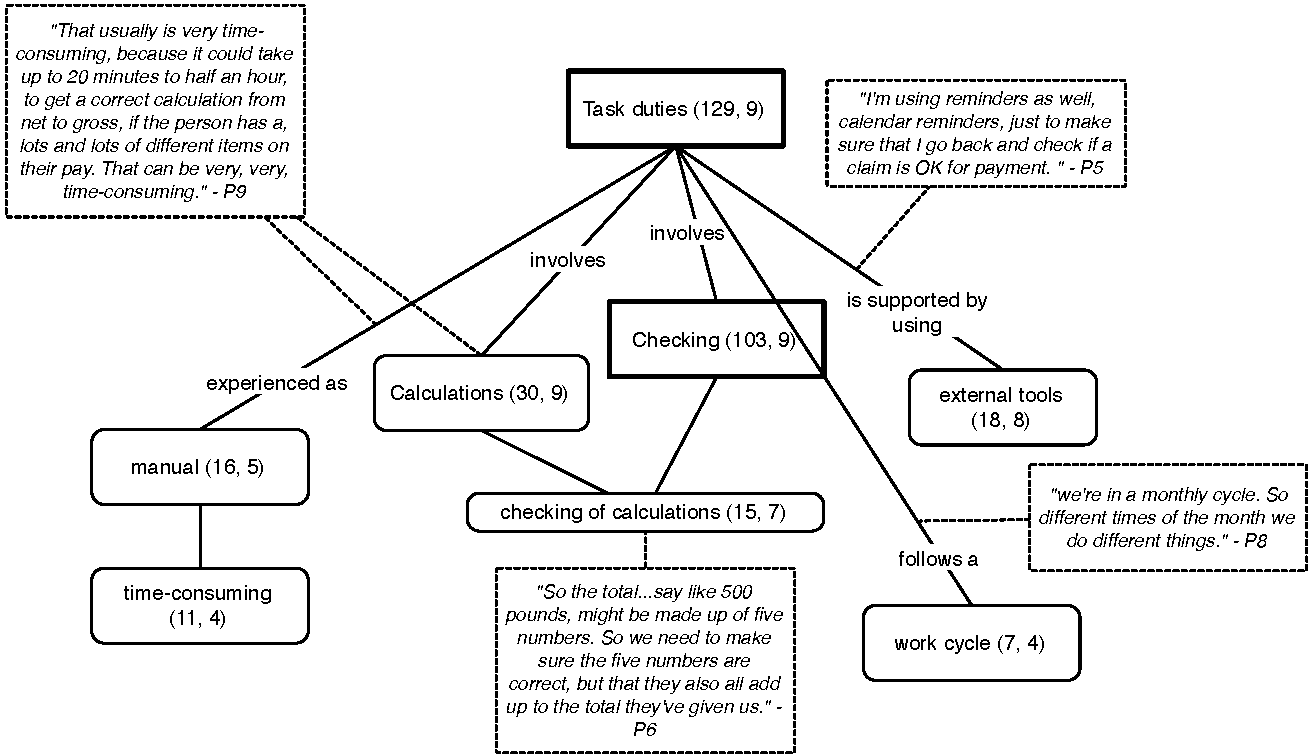
\includegraphics[width=\textwidth]{images/ch12/Task.pdf}
\caption[Study 1 Task diagram]{Diagram showing the theme Task. The numbers in parentheses indicate the number of quotes and the number of participants who mentioned it, respectively.}
\vspace{-9pt}
\label{fig:ch3_task}
\end{figure}

\section{Checking}\label{subsec:Checking}
Quotes were grouped under this theme if participants talked about checking data input as part of their job. 

\begin{figure}[!ht]
\centering
\includegraphics[width=\textwidth]{images/ch12/Checking.pdf}
\caption[Study 1 Checking diagram]{Diagram showing the theme Checking.}
\vspace{-9pt}
\label{fig:ch3_checking}
\end{figure}

\newpage

\begin{table}[htp]
\centering
    \begin{tabular}{ | l | p{10cm} |}
    \hline
     \textbf{Participant} & \textbf{Quote} \\ \hline
    P3 & \textit{"we try and pick it [errors] up and then obviously there's all the different stages that pick it up as you go along."}\\ \hline
    P9 & \textit{"the departments actually sometimes treat us as a checking system [laughs], but they shouldn't really, the schools. Because we're here just to make sure that people get paid correctly. But even though we are like a second check, we feel sometimes that we are the first checkpoint."} \\ \hline
    P7 & \textit{"All this piece of work, when we input in the system, will be actually checked by another person... my manager will print it out, and then check... other colleagues will double-check it for you as well, the calculations."} \\ \hline
    P8 & \textit{"one of these errors could be things that are missed during the checking."} \\ \hline

    \hline
    \end{tabular}
    \caption[Study 1 checking quotes]{Verbatim quotes taken from the interview transcripts that were about checking.}
    \label{table:ch3_checkingquotes}
\end{table}%

\begin{table}[htp]
\centering
    \begin{tabular}{ | l | p{10cm} |}
    \hline
     \textbf{Participant} & \textbf{Quote/note} \\ \hline
    P1 &  first puts in all the details, then when done checks everything against the source. \\ \hline
    P7 & when entering numbers from paper to computer, mostly looked at paper form and the number pad; only looked at screen after finishing entering all the numbers from the form to check. \\ \hline
    P5 & \textit{"We would go by the receipt, so we would try to make sure that the receipts are in order."} \\ \hline

    \hline
    \end{tabular}
    \caption[Study 1 checking own input]{Checking own input when entering data.}
    \label{table:ch3_owninputquotes}
\end{table}%

\begin{table}[htp]
\centering
    \begin{tabular}{ | l | p{10cm} |}
    \hline
     \textbf{Participant} & \textbf{Quote} \\ \hline
    P5 &  \textit{"The numbers on the expense form will be checked individually. So the total will obviously be, say like 500 pounds, might be made up of five numbers. So we need to make sure the five numbers are correct, but that they also all add up to the total they've given us."} \\ \hline
    P6 & \textit{"The numbers on the expense form will be checked individually."}\\ \hline
    P9 & \textit{"We have to check it one by one."} \\ \hline

    \hline
    \end{tabular}
    \caption[Study 1 checking other people's input]{Checking other people's input.}
    \label{table:ch3_otherinputquotes}
\end{table}%

\newpage

\section{System}
Quotes were grouped under this theme if participants talked about the computer system they were using to input data. 

\begin{figure}[!ht]
\centering
\includegraphics[width=\textwidth]{images/ch12/System.pdf}
\caption[Study 1 System diagram]{Diagram showing the theme System.}
\vspace{-9pt}
\label{fig:ch3_system}
\end{figure}

\section{Environment}
Quotes were grouped under this theme if participants described their environment, for instance if they talked about their physical work setting, and the work culture of their organisation. 

\begin{figure}[!ht]
\centering
\includegraphics[width=\textwidth]{images/ch12/Environment.pdf}
\caption[Study 1 Environment diagram]{Diagram showing the theme Environment.}
\vspace{-9pt}
\label{fig:ch3_environment}
\end{figure}

\newpage

\section{Data}
Quotes were grouped under this theme if participants described the data they were dealing with, for instance the type and length of data items, and from which source they copied data.

\begin{figure}[!ht]
\centering
\includegraphics[width=\textwidth]{images/ch12/Data.pdf}
\caption[Study 1 Data diagram]{Diagram showing the theme Data.}
\vspace{-9pt}
\label{fig:ch3_data}
\end{figure}

\section{Errors}
Quotes were grouped under this theme if participants described situations where errors were made: who made them, why were they made, what were the consequences. 

\begin{figure}[!ht]
\centering
\includegraphics[width=\textwidth]{images/ch12/Errors.pdf}
\caption[Study 1 Errors diagram]{Diagram showing the theme Errors.}
\vspace{-9pt}
\label{fig:ch3_errors}
\end{figure}

\newpage

\begin{table}[htp]
\centering
    \begin{tabular}{ | l | p{10cm} |}
    \hline
     \textbf{Participant} & \textbf{Quote/note} \\ \hline
    P6 &  \textit{"it's quite common that we have to return an expense or payment back to someone. It happens quite often, yeah."} \\ \hline
    P4 & Yes all the time, lots of typos.\\ 
    \hline
    \end{tabular}
    \caption[Study 1 errors quotes]{People mentioned errors occur quite frequently.}
    \label{table:ch3_occurrenceerrorsquotes}
\end{table}%


\begin{table}[htp]
\centering
    \begin{tabular}{ | l | p{10cm} |}
    \hline
     \textbf{Participant} & \textbf{Quote} \\ \hline
    P3 &  \textit{"sometimes it's because people have done typos, done too many zeroes, or left out a zero."} \\ \hline
    P5 & \textit{"the expense breakdown doesn't match what (...) whatever they put as the grand total."}\\ 
    \hline
    \end{tabular}
    \caption[Study 1 type of errors quotes]{The type of errors.}
    \label{table:ch3_typeoferrorsquotes}
\end{table}%


\begin{table}[htp]
\centering
    \begin{tabular}{ | l | p{10cm} |}
    \hline
     \textbf{Participant} & \textbf{Quote} \\ \hline
    P9 &  \textit{"Because the departments actually sometimes treat us as a checking system [laughs], but they shouldn't really."} \\ \hline
    P7 & \textit{"Yeah, human laziness or something [laughs]."}\\ \hline
    P8 & \textit{"sometimes, you know, through human error, you know, things don't get paid properly."} \\
    \hline
    \end{tabular}
    \caption[Study 1 reasons for errors quotes]{The reasons for errors.}
    \label{table:ch3_errorreasonsquotes}
\end{table}%


\begin{table}[htp]
\centering
    \begin{tabular}{ | l | p{10cm} |}
    \hline
     \textbf{Participant} & \textbf{Quote/note} \\ \hline
    P5 &  \textit{"generally we tend, we try not to send claims back to departments because they might get lost in the post, and it's an inconvenience as well. So we try to... resolve it ourselves.."} \\ \hline
    P4 & We allow a certain amount of tolerance; if it turns out the thing you bought has actually decreased value and is now  \pounds40, we will allow to return  \pounds50\\ \hline
    P7 & \textit{"we normally e-mail the budget holder to say... what you authorised is actually different. But for this kind of thing, it's only 10 pounds...we normally just process this without contacting them."} \\ \hline

    \hline
    \end{tabular}
    \caption[Study 1 acceptable errors quotes]{Acceptable errors.}
    \label{table:ch3_acceptableerrorsquotes}
\end{table}%

\clearpage
\section{Strategy}
Quotes were grouped under this theme if participants described the strategies they used to carry out their task.  

\begin{figure}[!ht]
\centering
\includegraphics[width=\textwidth]{images/ch12/Strategy.pdf}
\caption[Study 1 Strategy diagram]{Diagram showing the theme Strategy.}
\vspace{-9pt}
\label{fig:ch3_strategy}
\end{figure}

\begin{table}[htp]
\centering
    \begin{tabular}{ | l | p{10cm} |}
    \hline
     \textbf{Participant} & \textbf{Quote/note} \\ \hline
    P3 &  \textit{"I just try and do it in the quickest way...It's nice, once you've done it, it's completed, so it's sort your weight lifted [laughs]. So you don't need to think about it again."} \\ \hline
    P6 & \textit{"the expenses are done in a bulk, rather than separated over a period of time. When I'm doing it lots at a time, I think once you get into sort of the hang of it, it gets done a lot quicker than..you just get used to putting them in, and inputting it all."} \\ \hline
    P9 & \textit{"I try to concentrate on my task...I try to do one task [i.e. doing all expenses], finish one, and then do another."} \\ \hline
    P4 &  It's difficult to take rests or even switch in-between number entry tasks because of the work pressure, and feels pressure by boss. \\ 
    \hline
    \end{tabular}
    \caption[Study 1 batching quotes]{Most participants entered all numbers in one go.}
    \label{table:ch3_inonegoquotes}
\end{table}%

\begin{table}[htp]
\centering
    \begin{tabular}{ | l | p{10cm} |}
    \hline
     \textbf{Participant} & \textbf{Quote/note} \\ \hline
    P3 &  \textit{" I wouldn't necessarily have to [memorise numbers], It's more just if you have to keep flicking back to different things, it's sometimes just easier to write it down, or just try and remember it. But you can obviously take the long version and keep flicking back to the correct screen."} \\ \hline
    P2 & \textit{"we have different grants and different project codes as a result, but you, because you use them so much, you end up remembering them."} \\ \hline
    \end{tabular}
    \caption[Study 1 strategy quotes]{Examples of strategies people used.}
    \label{table:ch3_strategiesquotes}
\end{table}%

\ \clearpage

\section{Importance of accuracy and paper trails}
Quotes were grouped under this theme if participants talked about the sensitivity of financial data, which is why not all people were authorised to approve or access financial data, and the importance of a paper trail for data entries. 

\begin{figure}[!ht]
\centering
\includegraphics[width=\textwidth]{images/ch12/Papertrail.pdf}
\caption[Study 1 Importance of accuracy and paper trails diagram]{Diagram showing the theme 'Importance of accuracy and paper trails'.}
\vspace{-9pt}
\label{fig:ch3_papertrail}
\end{figure}

\section{Other}
Quotes were grouped under this theme if participants talked about things that did not fit into any other category but were still considered relevant, such as issues participants experienced, or queries they often received.

\begin{figure}[!ht]
\centering
\includegraphics[width=\textwidth]{images/ch12/Other.pdf}
\caption[Study 1 Other diagram]{If people described issues, it usually had to do with the system.}
\vspace{-9pt}
\label{fig:ch3_other}
\end{figure}

\begin{table}[htp]
\centering
    \begin{tabular}{ | l | p{10cm} |}
    \hline
     \textbf{Participant} & \textbf{Quote/note} \\ \hline
    P5 &  \textit{"There are other issues. You could say I think hundreds, I mean not just with the work that we do on expenses, but across [university A], across [university A] Finance, the Finance division...We just have to kind of work our way around the system and you know, adapt to it."} \\ \hline
    P7 & \textit{"It's only the matter of how you get used to the Payroll system. Because companies have different systems, the data inputting can take a while to get used to it."} \\ \hline
    P9 &  \textit{"You know, all systems are a bit funny, I think. But you just gotta get used to it."} \\ \hline
    \end{tabular}
    \caption[Study 1 issues quotes]{Issues that participants experienced with the system.}
    \label{table:ch3_otherquotes}
\end{table}%


\chapter{Information sheet}\label{ch:information_sheet}
The information sheet given to the participants in Study 1 is shown in Figure \ref{fig:informationsheet}. 

\begin{figure}[htp] \centering{
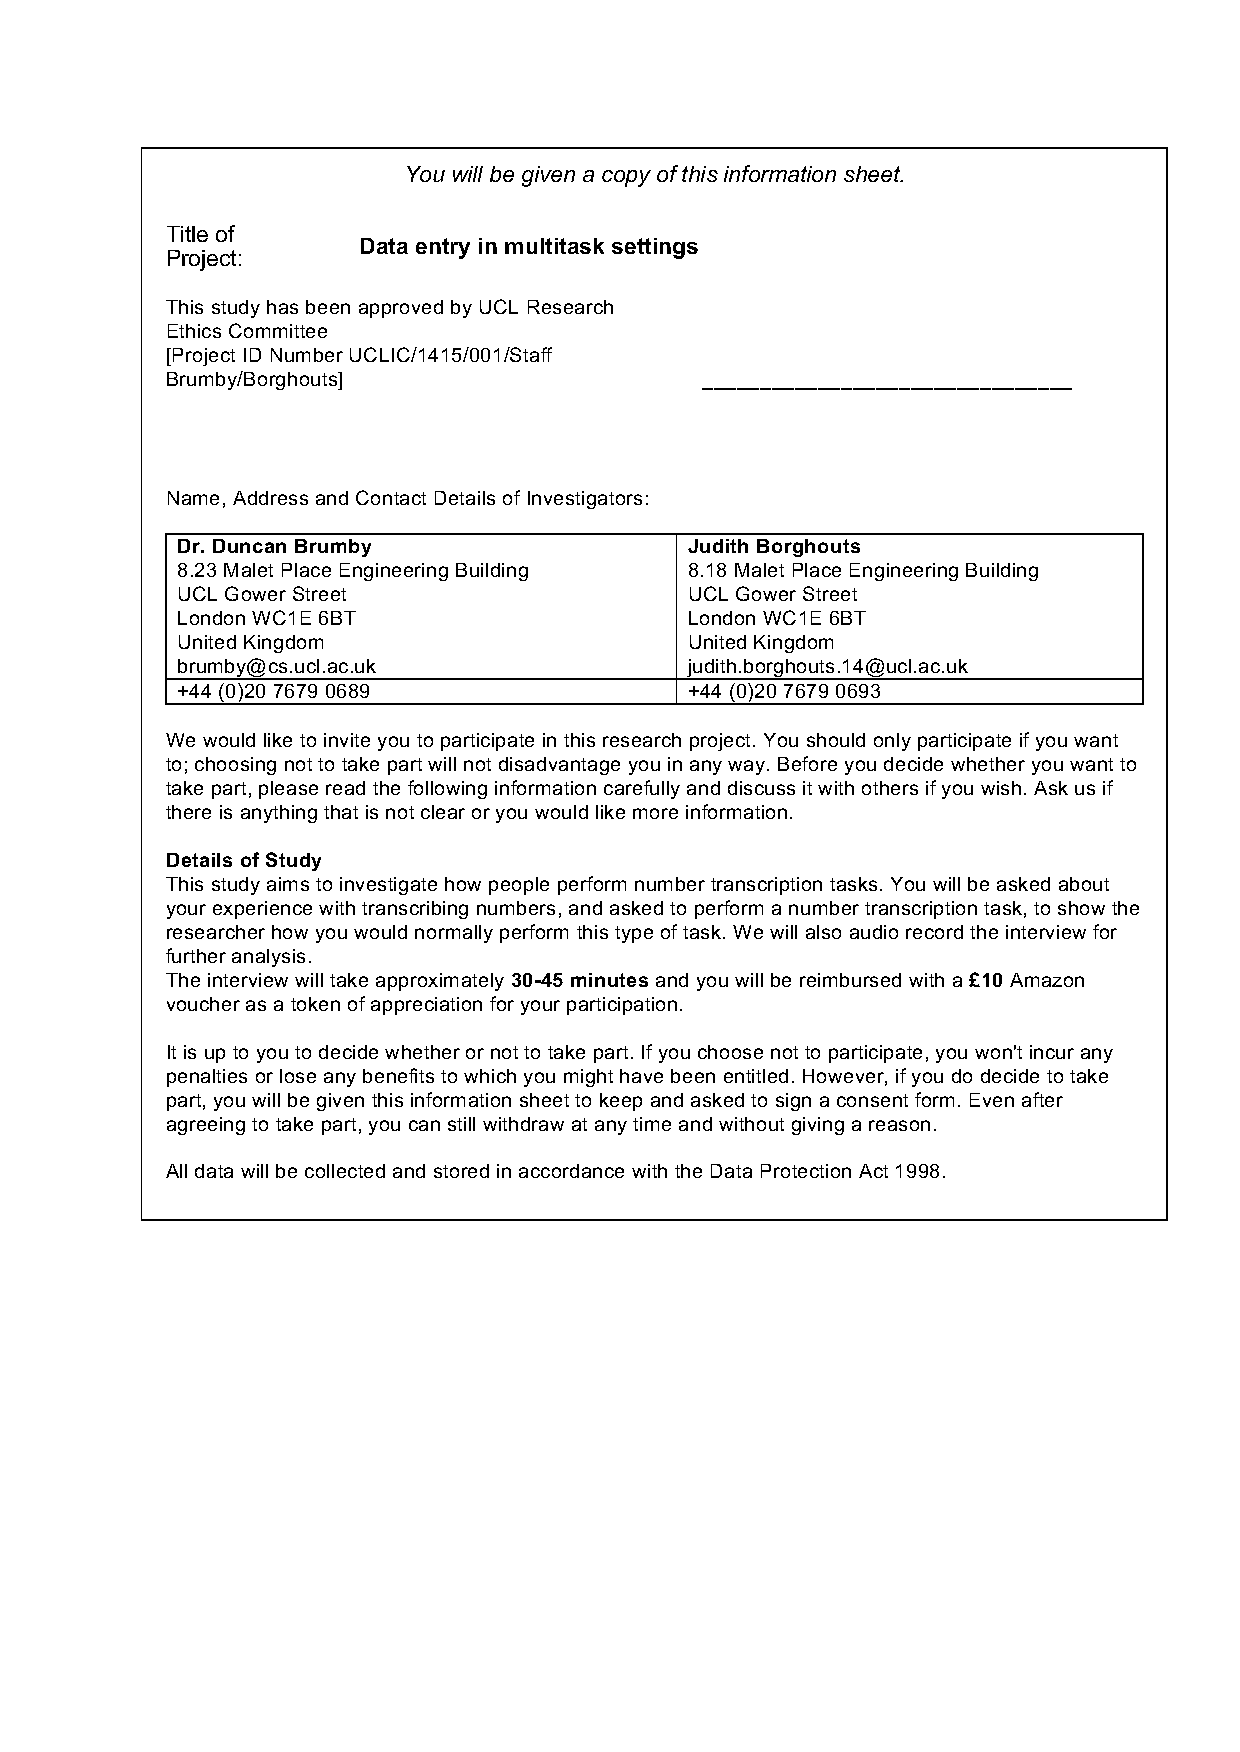
\includegraphics[width=\textwidth,keepaspectratio]{images/Informationsheet.pdf}}
\caption{Information sheet}
\label{fig:informationsheet}
\end{figure} 

\chapter{Consent form}\label{ch:consentform}
The consent form used for Study 1 is shown in Figure \ref{fig:consentform}. 

\begin{figure}[htp] \centering{
\includegraphics[width=\textwidth,keepaspectratio]{images/Consentform.pdf}}
\caption{Consent form}
\label{fig:consentform}
\end{figure} 

\chapter{Interview script}\label{ch:interviewscript}
The interview script used for Study 1 is given below. This script only served to guide the interview, and does not contain all questions that were asked. Based on what the participant was saying, follow-up questions were asked. 

\subsubsection{Before the interview}
\begin{itemize}
\item 
ensure participant is aware of purpose research 
\item 
explain what will happen
\item 
informed consent
\item 
ask for permission to audio record interview
\end{itemize}
\subsubsection{Work}
\begin{itemize}
\item Tell me something about your work (what do you do)
\item  How many hours per week (full-time/part-time)
\item How long have you been working here (at this company) \item How long have you been doing this type of work
\end{itemize}
\subsubsection{Number entry}
\begin{itemize}
\item  What activities do you do for work that involve transcribing numbers?
e.g. filling in expenses, tax returns, setting up invoices
\item How often do you do this (per day/week)?
\item How many numbers is it roughly that you have to enter?
\item How long do you usually take?
\item What type of numbers? Usually same numbers, or can it be anything?
\item Do you get to enter numbers that are different from your familiar format?
e.g. 2,000 or 2.000; 9/15/14 instead of 15/9/14
\item Do you deal with foreign currencies?
\item Tell me something about how you enter these numbers
\item When do you do these tasks? Immediately when you get them, or save them for later? Morning, afternoon?
\item Does urgency/time pressure influence how you do the task (if so, how)
\item Do you do them in-between other tasks or save a particular part of the day for it?
\item Do you do all tasks all at once, or take rests in between?
(if rests, what do you do? switch to another task, have a coffee, lunch, break, etc.)
\item Do you feel that the way you enter it changes after a while?
e.g. you get better at it so it kind of becomes automatic, or less mentally exhausting? Or is it the opposite, becomes more exhausting?
\item Do you do other things as well during this task
e.g. listening to music, attending to another task
\item Do you sometimes have to briefly store numbers in memory, or calculate them from numbers you already have?
If so, do you use external tools to offload memory?
\item Where do you copy them from? Paper, digital files, combination?
\item Do numbers get checked, to see if they're correct? Do you or anyone else check these numbers?
\item Do you ever get entered numbers from someone else, that you then have to check if they are correct?
\item What is your general experience with transcribing numbers?
e.g. easy, boring, part of the job
\end{itemize}
\subsubsection{Environment}
\begin{itemize}
\item Do you always work in the same environment, or sometimes work in different places, such as at home, or when you're on the train, or working at a cafe? What about number entry tasks?
\item Do you do your work on a desktop, laptop, tablet, anything else? Are some devices harder or easier?
\item How is your desk organized?
\item Do you organise it differently when doing number entry tasks?
\item Do you have notifications on (e.g. e-mail, work-related instant messaging); if you do get new notification, do you attend to it straight away or finish task first?
\item Do you get interrupted in other ways, for example when the phone is ringing, or when a colleague or your boss asks you something? How do you deal with these interruptions? What is your experience with these interruptions?
\item Critical incident: Has there ever been an incident where a mistake in entering a number went undetected, and was discovered later on?
\end{itemize}
\subsubsection{Demonstration}
\begin{itemize}
\item Could you show me the software you use to transcribe numbers?
What is your experience with this system, works well?
(If negative, how do you deal with that? do you use any strategies to make it more optimal for yourself?)
\item Do you feel confident entering the numbers?
\item How do you place your windows?
\item Could you show me how you perform a typical number transcription task (do it how you would normally); if you feel uncomfortable about sharing work data, you can enter any type of numbers, as long as it somewhat resembles data you would normally enter for work
\end{itemize}
\subsubsection{After the interview}
\begin{itemize}
\item Thank participant
\item explain what will happen to their data
\item do they have any more questions
\item clarify when they will be compensated
\item Ask if participant knows any further people who might be suitable and willing to participate
\end{itemize}

\chapter{Study 2: Distributed Cognition models}\label{ch:S2_Models}\label{ch:S2_Models}
To aid the analysis of the contextual inquiry data collected in Study 2, I developed three Distributed Cognition models using \citet{Furniss2006}'s guidelines:

\begin{itemize}
\item 
The physical model: this model describes the physical layout of the task environment
\item 
The information flow model: this model describes how information flows through all users involved in the task
\item 
The artefact model: this model describes all artefacts involved in the task
\end{itemize}

These models were used to gain insight how information sources were distributed in the task environment, and were used to understand differences in inquiries. Each model consists of a diagrammatic representation that visualises the data, and a narrative representation which verbally describes the data. 

The three models are described below. I used the DC principles as described by \citep{Furniss2006} as guidelines to decide what to include in the models. The principles of each model are described at the start of each section, and marked in italics (e.g., \textit{horizon of observation}) in the narrative descriptions.

\section{Physical model}
\begin{figure}[!ht]
\centering
\includegraphics[width=0.3\textwidth]{images/ch12/ch12_physmodroom.pdf}
\caption[Study 2 Room model]{Physical model diagram showing a typical physical layout of people's work environment at room level.}
\vspace{-9pt}
\label{fig:ch12_physmodroom}
\end{figure}

\begin{figure}[!ht]
\centering
\includegraphics[width=0.3\textwidth]{images/ch12/ch12_physmoddesk.pdf}
\caption[Study 2 Desk model]{Physical model diagram showing the physical layout of people's work environment at desk level.}
\vspace{-9pt}
\label{fig:ch12_physmodroom}
\end{figure}

The physical model describes what the individual can physically hear, see, and access, and how information sources are laid out in the physical environment. In developing the model the following was considered: what is the proximity of, and access to, devices and people: what can be seen and heard from the individual's point of view?

\begin{framed}\noindent
\textbf{Physical model principles}

\begin{itemize}
\item Space and Cognition: how do people use the physical space to support their work
%\item Perceptual principle: what is the mapping between the spatial layout of information, and that which it represents
%\item Naturalness principle: does the form of how information is represented match the properties of what it represents
\item Subtle bodily supports: do people use their body to support their work
\item Situation awareness: are people informed of what is going on
\item Horizon of observation: what are people able to see and hear
\item Arrangement of equipment: how do people arrange their equipment
\end{itemize}

\end{framed}

%Physical layout
The physical layouts of the four offices were not identical, but shared a number of characteristics. All participants had their own desk and worked in an open office with two or more colleagues. P3 was the only person in the office responsible for data entry tasks. The other eight participants had colleagues in the same room who dealt with similar tasks. P1, P2, P8 and P9 also had colleagues in the same room that worked on different tasks. Colleagues that were working on different tasks were situated further away from them than other colleagues. As an example, the physical environment of the office of P1 and P2 is depicted in Figure \ref{fig:ch12_physmodroom} at room (a) and desk (b) level. The number of people in one room ranged from two to sixteen. 

The open layout made it easy for colleagues to interact with each other and share information between themselves. They could see when a colleague was present and available to consult. Participants regularly consulted colleagues in their room to retrieve information they could not find on any other sources. This information is given verbally, or a colleague directs the participant to the correct information source.

The offices had an open-door policy, meaning that workers could at any time be interrupted by people walking in. During the observations, participants were regularly interrupted by colleagues. They responded to it but used \textit{subtle bodily supports} to not lose track of where they were in the expenses task. For example, P3 responded verbally to a colleague but kept his kept his visual attention on the computer and tried to continue with the expenses task. When P1 was interrupted by a colleague, he placed a finger on the computer screen to remember where he was in the task.

%Sometimes it is colleagues at the same level of processing, sometimes it is people who are higher in the task hierarchy. For example, a boss who needs to check another colleague'��s entries can be collocated around a desk and query this colleague if something is incorrect. They can also view how many of the outstanding claims still need to be processed as they are on their colleague's desk.

%SOURCES
All participants worked with both paper and digital information sources. Several participants used the physical \textit{space} to organise their paper sources. P2 maintained separate physical locations on his desk for expense claims to be processed, expense claims that had been completed, and exceptional claims that required further attention. P7 also had paper sources fixed on his wall, which were visible from his desk. 

Other physical sources were located in an individual's drawer, in a shared bookcase or drawer in the same physical room. These were not visible from their desk, and participants had to physically move from their desk to retrieve and view this information. Participants could see whether a colleague is present or not, and whether they can consult them at that moment to request information. Recent physical files are kept in a closet in the same room, whereas older files and employee files are physically kept in another location. These older files were used less frequently.
If P6 received expense claims, she placed these in her drawer to return to later. If there were a lot of claims to be processed or if the participant started processing claims, these were placed on their desk. 

Participants become aware of new claim requests by batches of claim forms or receipts on their desk with a handwritten note, the claimant asking them in person, or when they check their e-mail and see a new e-mail by the claimant. For physical claims, they browse through them and place them either at a dedicated area on their desk or in their drawer, to return to later. P2, P3 and P6 re-ordered claims based on urgency. Claims that were more urgent were processed first. These could be claims by their boss, or claims with an explicit instruction that it was urgent. In addition, P2 sometimes grouped claims according to category. The reason for grouping them is that different categories of expenses can require other data fields to be filled in, and P2 felt it to be easier to do these particular type of claims together. Examples are travel expenses for which participants have to fill in the departure point and destination, or external lunches for which the name of the restaurant has to be filled in. Participants place exceptional claims in a separate physical location. For P2, this was in a separate tray in the top-left hand corner of his desk. By putting it in his \textit{horizon of observation}, he can see if there are still claims in this tray to be processed and return to at a later point in time. P2 starts each day by seeing if there are claims in this tray, and processes these first. P5 places exceptional claims in a separate drawer. They are not visible and she does not use any reminders, but returns to these when she sees fit.

Participants also received requests digitally through email. They could not place these in their horizon of observation. However, whether the claim requests were in physical or digital form, they always needed the physical receipts of expenses, before they could process a claim. Similar to physical claim forms, they had these receipts either in their drawer or on their desk, as a reminder that they still needed to process these claim requests.

Participants also created their own artefacts to aid them in their work. This includes physical artefacts, such as a spreadsheet with frequently used codes, as well as digital artefacts, such as a digital form to look up codes by person name. Participants could type in a name of a claimant, and the form populated codes related to one person. This made it easier for people to look up which account codes to charge the expenses to. 

Digital information sources included the data entry system, intranet, and external websites via their computer. Furthermore, they had digital files, such as PDF files, Excel spreadsheets, and Word documents stored on their desktop computer. The \textit{arrangement of equipment} was that seven out of nine participants had two screens. All seven participants mainly used one screen, both to enter and retrieve information. Some participants used a second screen to display their email inbox. If they received a notification of a new email, they would briefly glance to determine the urgency and importance of the email, but would try to continue with the expenses task. 

Sometimes a claim was checked by multiple people in the same room. Participants had \textit{situation awareness} of the progress of the claim as long as it was still in the same physical office. They could see the progress of expense claims by the pile on colleagues' desks, and could ask colleagues in person. Furthermore, they can overhear conversations on the phone and become aware of claims that require further attention. Participants can see their own screens and desks. They have to walk over or do additional physical actions in order to view what is on colleagues' desk.  

As soon as an expense claim was submitted to another office and physical location, the user would have little \textit{situation awareness} of the progress of the claim. The system did not have a visible status update, meaning participants can not see the progress of their claim once it has been submitted to Central Finance. As they do not receive updates, administrators and claimants often forget to keep paying attention to it and do not query it until they realise payment has not been processed yet. Often an error will have occurred and at this point the project may have finished and payment is no longer possible. If participants needed more information on the status of a claim, they needed to contact colleagues from another office via email and telephone, or they had to visit the other physical location.  Participants called colleagues from other departments with queries such as errors, and outstanding claims that had not been processed yet. They emailed claimants with queries such as if they do not agree with the expenses claimed, if they need further information, or if they have spotted an error.


%\begin{table}[htp]
%\centering
%\begin{tabular}{  l }
%\hline
%\textbf{ Physical} \\  
%Paper receipts \\  
%Personal files of employees \\  
%Written instructions by claimants \\  
%Paper claim forms \\
%Calculator \\
%Documents created by the participant
%\vspace{10pt} \\
%
%\textbf{Digital} \\ 
%E-mails \\ 
%The expenses entry system \\ 
%Excel spreadsheets \\ 
%Intranet \\ 
%External websites \\ 
%PDF files \\ 
%Calculator \\ 
%Documents created by the participant
%\vspace{10pt} \\
%
%\textbf{Other} \\ 
%Colleagues \\ \hline
%
%\hline
%\end{tabular}
%\caption[Study 2 information sources]{The information sources people needed for expenses tasks.}
%\label{table:ch12_infsources}
%\end{table}


\section{Artefact model}
The artefact model describes the artefacts that are used. 

\begin{framed}\noindent
\textbf{Artefact model principles}  \\
\begin{itemize}
\item Mediating artefacts: do people use any artefacts to support their work
\item Creating scaffolding: do people use the environment to simplify tasks, e.g. set reminders
\item Representation:goal parity: do people use artefacts to display the explicit relationship between the current and goal state of their work
\item Coordination of resources: how do people coordinate their information
\end{itemize}
\end{framed}

%. Participants have access to their intranet, where project information for the department such as project codes are stored. 

Participants work with both physical and digital artefacts. Table \ref{table:ch12_infsources} shows an overview of the information sources that were involved in an expenses task. For each instance of the task, several artefacts can be used, but there are two main artefacts that are used in each instance and are central to the expenses task: the paper receipts and the expenses entry system.
In addition to information sources, participants use several \textit{mediating artefacts} to support their work. Calculators are used to aid in calculating sums. Multiple tools were consulted to convert currencies: an external website, a tool on the intranet, and a tool included in the data-entry system itself. They use a physical tray on their desk to hold exceptional claims. They use a pen to annotate receipts and highlight which items on receipts to claim back.

Some of the participants \textit{created external scaffolding} to simplify their task. In particular, participants had difficulties remembering codes they needed to enter. P5 and P6 had made a personal spreadsheet with codes they used most frequently. P4 remembered old codes but had difficulties remembering new codes since they had changed 18 months ago. To look up codes, she used a spreadsheet created by the departmental manager where she could fill in old codes, that would populate the correct new code. 

\textit{The parity between the current and goal state} was displayed on the expenses system. Once a claim had been submitted, there would be a status update in the expenses system. This status reveals whether a claim is Pending, has been Paid, or whether Original receipts are required. As long as a claim was Pending however, there was however no insight into what is happening on the other side. Often a claim would be received but would be held because there was information missing. Participants would not know about this unless they explicitly contacted the office, and depending on the situation, they would often still not receive information on what was happening with a particular claim because the information was not centralised in Central Office and the person on the phone would not be able to look up what was happening with a particular claim.

In order to \textit{coordinate resources}, the intranet was intended as a central point for claimants, administrators and Central Finance officers to access the same information resources. Participants find the resources difficult to use, so people often end up making their own local copies and working with these instead. This supports them better in their work, but they can end up working with old and incorrect information if information gets updated. Examples of information sources used locally are claim forms: claimants keep working with local copies on their computer and do not download the new forms. They keep using old information such as old salaries and old project codes. Another example are spreadsheets with budget codes: administrators created and used their own spreadsheets with codes. If codes were updated, they were not aware and ended up working with old codes. 
There was an instruction manual to do expenses, to ensure everyone carried this routine task in the same way. Newcomers usually learnt how to do it from other people rather than this written manual, as the experience was that it was often easier and faster to learn it this way. This way of learning the activity again had the risk that some people were doing it in the old, incorrect way, and passed on this incorrect way of doing work to others.
In order to provide proof of expenses, people still had to provide hard-copy receipts. These need to be sent to Central Finance, but often get damaged and lost and the claimant and administrator will not know, but Central Finance will not know either so nothing will happen unless the administrator or claimant takes action and chases it. 

In order to prevent people from interrupting an expenses task, people were logged out of the data entry system after a period of inactive use and they had to restart the task from the beginning. This added cost to resume the task kept participants focused on the data entry task, and they were less likely to interrupt and switch to unrelated tasks. However, people often did not know beforehand what the cost to access information was going to be. Furthermore, it was also not clear after how long the timeout would occur [quote].

\section{Information flow model}
This model describes the flow of information through several actors for an expenses task.

\begin{framed}\noindent
\textbf{Information flow principles}
\begin{itemize}
\item Information movement: how does information move throughout the system
\item Information transformation: does the representation of information undergo changes
\item Information hubs: what are the main points where different information channels meet
\item Buffering: are there any buffers to uphold information
\item Communication bandwidth: how does communication take place
\item Informal communication: does informal communication take place in addition to formal communication
\item Behavioural trigger factors: are there any local factors that individuals respond to
\end{itemize}
\end{framed}

\begin{figure}[!ht]
\centering
\includegraphics[width=0.3\textwidth]{images/ch12/ch12_infmodel.pdf}
\caption[Study 2 Information flow model]{Model of the information flow.}
\vspace{-9pt}
\label{fig:ch12_infmod}
\end{figure}


An expenses claim \textit{moves} through several actors, and moves between actors via email, phone, physical post, and face-to-face communication. The actors who contribute to the processing of an expense claim have limited visibility on the overall status and progress of the claim. For example, once claimants submit a claim request to the administrator, they do not know what the status is of that claim until they receive an email notification that it has been completed. Similarly, once administrators submit a claim to the Central Finance office, they do not know what the status is of the claim. They do not know when or whether it has been processed and if not, what the reasons are for holding it. The workers at the Central Finance office know the reasons for withholding a claim, but often receive incomplete information of a claim, and for example do not know the justification behind a claim, whether the expenses are made correctly and if there is an error in the project code entry, they do not know the correct project to charge it to.

\textit{Information transformation} takes place when calculations have to be carried out. At the beginning the individual numbers are saved, as well as the calculations on those numbers. Once a claim is submitted only the end result will be saved on the system. For example, if one claim request involves multiple expenses, each individual amount has to be checked by the administrator. Administrators are then free to choose whether to type each amount or only the sum total on the system. Once they have processed and submitted the claim, only the sum amount will be available for auditors. 

There are two main \textit{information hubs}: the first hub is the office of the administrator, who deals with incoming claims and hard-copy receipts from claimants. These claims are processed at the administrator office and then sent off to the Central Finance office, the second information hub. Workers at this office deal with incoming claims and hard-copy receipts from administrators, match and process these and submit them for payment. 

The administrator is the main\textit{ information buffer }between the claimant and the Central Finance officers. Claimants submit a request to administrators. This claim is upheld until the administrator decides to process it and send it to Central Finance. If there was an issue with a claim, claimants contacted the administrator, who then contacted Central Finance. Though claimants could also contact Central Finance directly, administrators said it was often easier if they contacted Central Finance on their behalf, as they knew who to contact [quote]. 

\textit{Communication} between the claimant and administrator takes place face-to-face, over the phone, via email and via handwritten notes. Communication between colleagues takes place face-to-face. Communication between the administrator and Central Finance solely takes part via email or over the phone, though it is possible to take place face-to-face.

Instructions are mostly \textit{communicated informally} through word of mouth. Knowledge of how to use the system sits with the employees, and it is often faster to explain newcomers how to do it rather than go through the written instructions. A consequence is that when information gets updated, not everyone is aware of it and keeps using the old and incorrect way, or learn the incorrect way from someone else who is still using the old way. 

Receiving a claim request from another actor are the main \textit{factors triggering behaviour.} Participants collected claim requests and saved them to return to later. Some participants kept claims to be completed on their desk. The size of this pile acted as a trigger to decide whether to start processing them. Furthermore, the payroll deadline was another trigger. Participants tried to complete claims before the deadline so claimants were reimbursed in time.

\chapter{Study 4: interleaving rates per participant}\label{ch:S4_PartPlots}
Study 4 investigated the effect of time costs on the timing of inquiries. For this purpose, on a trial-by-trial basis it was considered whether participants entered expenses in sequential order, or whether they entered items with a low cost of each expense first. Across conditions, participants were mostly consistent in strategy choice, and interleaved on either all or no trials. The consistency in strategy choice per participant is further illustrated in Figure \ref{fig:ch34_4-plotpp}, which displays a plot for each participant across trials. The x axis plots the trial number, and the y axis displays whether they interleaved on that trial or not: a value of 0 means they did not interleave, and a value of 1 means they did interleave. These plots further illustrate that most participants were consistent in interleaving on no or all trials, as the majority of plots have a flat line (see for example Participant 6, who interleaved on all trials). A subset of participants switched between strategies at the first couple of trials before sticking with one strategy, such as Participants 9 and 12: at the start of the x axis, their lines go up and down between 0 (no interleaving) and 1 (interleaving) before becoming a straight line. Lastly, participants 29, 32 and 33 seemed to switch between the strategies throughout the experiment and did not stick with a particular strategy: their lines continue to go up and down between 0 and 1 along the entire x axis. 

\begin{figure}[!htbp]
    \centering
    \begin{subfigure}[b]{0.5\textwidth}
        \includegraphics[width=\textwidth]{images/ch34/ch34-4_plotControl(1).png}
        \includegraphics[width=\textwidth]{images/ch34/ch34-4_plotControl(2).png}
        \caption{Participants in the Control condition.}
    \end{subfigure}
    ~ %add desired spacing between images, e. g. ~, \quad, \qquad, \hfill etc. 
      %(or a blank line to force the subfigure onto a new line)
    \begin{subfigure}[b]{0.5\textwidth}
        \includegraphics[width=\textwidth]{images/ch34/ch34-4_plotHigh-Am(1).png}
         \includegraphics[width=\textwidth]{images/ch34/ch34-4_plotHigh-Am(2).png}
        \caption{Participants in the High-Amount condition.}
    \end{subfigure}
        \begin{subfigure}[b]{0.5\textwidth}
        \includegraphics[width=\textwidth]{images/ch34/ch34-4_plotHigh-Acc(1).png}
         \includegraphics[width=\textwidth]{images/ch34/ch34-4_plotHigh-Acc(2).png}
        \caption{Participants in the High-Account condition.}
    \end{subfigure}
    ~ %add desired spacing between images, e. g. ~, \quad, \qquad, \hfill etc. 
    %(or a blank line to force the subfigure onto a new line)
    \caption{A plot per participant across trials. The x axis shows the trial number, and the y axis indicates whether a participant interleaved on a trial: a value of 0 means they did not interleave, a value of 1 means they did interleave.}\label{fig:ch34_4-plotpp}
\end{figure}
\end{appendices}

\end{document}